\documentclass[fleqn, 11pt, color=blue]{elegantbook}
\usepackage{parskip}  % Adds space between paragraphs and removes indentation
\usepackage{tikz}
\usepackage{graphicx}
\usetikzlibrary{shapes.geometric} % Add this line
\usetikzlibrary{arrows.meta, positioning} % For better arrowheads
\usepackage{circuitikz}
\usetikzlibrary{circuits.logic.US}
\usepackage{mymacro}
\usepackage{pgfplots}
\usepackage{pgfplotstable} % Needed to read data tables
\usepackage{booktabs} % For professional-looking tables
\usepackage{colortbl} % For coloring table rules


% Reset any color scheme
\color{black} % Ensure text color is black
\pagecolor{white} % Ensure page color is white


\usepackage{pgfplots}
\pgfplotsset{compat=1.18}

\usepackage{listings}
\usepackage{xcolor}

% Customise the listing caption to "Algorithm"
% Define custom style for Python code
\lstdefinestyle{pythonStyle}{
  language=Python,
  basicstyle=\ttfamily\small,
  keywordstyle=\color{blue}\bfseries,
  commentstyle=\color{gray},
  stringstyle=\color{red},
  numbers=left,
  numberstyle=\tiny\color{gray},
  stepnumber=1,
  numbersep=5pt,
  showspaces=false,
  showstringspaces=false,
  frame=single,
  breaklines=true
}

% Define custom style for Java code
\lstdefinestyle{javaStyle}{
  language=Java,
  basicstyle=\ttfamily\small,
  keywordstyle=\color{purple}\bfseries,
  commentstyle=\color{gray},
  stringstyle=\color{red},
  numbers=left,
  numberstyle=\tiny\color{gray},
  stepnumber=1,
  numbersep=5pt,
  showspaces=false,
  showstringspaces=false,
  frame=single,
  breaklines=true
}

% Customise the listing caption name
\renewcommand{\lstlistingname}{Algorithm}


% Define a style for inline Java code
\newcommand{\inlinecode}[1]{\lstinline[language=Java, basicstyle=\ttfamily\small]{#1}}

% Override the colors used in the clrscode4e package
\definecolor{commentcolor}{cmyk}{0, 0, 0, 1} % Change comment color to black
\definecolor{linenumcolor}{cmyk}{0, 0, 0, 1} % Change line number color to black

\usepackage{array,mathtools}
\newcommand*{\carry}[1][1]{\overset{#1}}
\newcolumntype{B}[1]{r*{#1}{@{\,}r}}
\usepackage{lmodern}

% Define skewed overline
\newcommand{\myol}[2][3]{{}\mkern#1mu\overline{\mkern-#1mu#2}}

\newcommand{\floor}[1]{\left\lfloor #1 \right\rfloor}



\usetikzlibrary{matrix}

\newcommand{\addend}{\text{\textsl{\color{gray}{Addend}}}}
\newcommand{\augend}{\text{\textsl{\color{gray}{Augend}}}}
\newcommand{\sumOut}{\text{\textsl{\color{gray}{Sum}}}}
\title{Mathematics for Software Engineering}

\author{Richard Brooks \& Eduard Fekete}
\date{May, 2025}
\version{2.0}

\cover{cover4.png}

% modify the color in the middle of titlepage
\definecolor{customcolor}{RGB}{108, 162, 198}
\colorlet{coverlinecolor}{customcolor}

\newcommand{\mycircled}[1]{\tikz[baseline=(char.base)]{
            \node[shape=circle,draw,inner sep=2pt] (char) {#1};}}
            

\usepackage{nccmath, mathtools}
\usepackage[dvipsnames]{xcolor}
\usepackage{hyperref}
\usepackage{subcaption}


%======================================================================
% FINAL, CORRECT SOLUTION FOR AUTOREF NAMES IN ELEGANTBOOK
% This works by defining the internal counter names that hyperref needs.
% Place this block in the preamble of your main.tex file.
%======================================================================
\makeatletter
\AtBeginDocument{%
  \def\tcb@cnt@definitionautorefname{Definition}%
  \def\tcb@cnt@theoremautorefname{Theorem}%
  \def\tcb@cnt@lemmaautorefname{Lemma}%
  \def\tcb@cnt@corollaryautorefname{Corollary}%
  \def\tcb@cnt@propositionautorefname{Proposition}%
  \def\tcb@cnt@axmautorefname{Axiom}%
  \def\tcb@cnt@postulatenameautorefname{Postulate}%
  \def\examautorefname{Example}%
  \def\exerautorefname{Exercise}%
  \def\probautorefname{Problem}%
  \def\remarkautorefname{Remark}%
}
\makeatother
%======================================================================

% Redefine the example environment to add vertical spacing before it
\makeatletter
\renewenvironment{example}[1][]{%
  \vspace{1em}% Add vertical space before the example
  \refstepcounter{exam}%
  \par\noindent\textbf{\color{main}{\examplename} \theexam #1 }\rmfamily}{%
  \par\ignorespacesafterend}
\makeatother

% MSE Colors - Matching the MkDocs website
% This file contains color definitions matching the MkDocs site: MSE1_DK_25

%% Light Mode Colors
\definecolor{mseViaBlue}{RGB}{108, 162, 198}    % #6CA2C6 - VIA blue for links/accents
\definecolor{mseOrange}{RGB}{255, 140, 0}       % #FF8C00 - Orange accent
\definecolor{mseDarkText}{RGB}{54, 54, 54}      % #363636 - Default text color
\definecolor{mseBackground}{RGB}{255, 255, 255} % #FFFFFF - Background

%% Dark Mode Colors
\definecolor{mseDarkBg}{RGB}{13, 16, 23}        % #0d1017 - Dark background
\definecolor{mseDarkBlue}{RGB}{18, 49, 97}      % #123161 - Header/active elements
\definecolor{mseGlowBlue}{RGB}{42, 157, 244}    % #2A9DF4 - Glow/secondary blue
\definecolor{mseLightBlue}{RGB}{60, 172, 248}   % #3CACF8 - Light blue accent
\definecolor{mseDarkText}{RGB}{192, 212, 240}   % #C0D4F0 - Dark mode foreground text

%% Admonition Colors
\definecolor{mseQuestionBorder}{RGB}{45, 180, 153}   % #2DB499 - Question green
\definecolor{mseQuestionBg}{RGB}{204, 241, 234}      % #CCF1EA - Question background
\definecolor{mseAnswerBorder}{RGB}{229, 171, 72}     % #E5AB48 - Answer orange
\definecolor{mseAnswerBg}{RGB}{255, 239, 211}        % #FFEFD3 - Answer background

%% Set Number Theory Colors (for Venn diagrams, etc)
\definecolor{mseNaturals}{RGB}{255, 150, 50}       % BurntOrange - Natural Numbers
\definecolor{mseIntegers}{RGB}{255, 120, 70}       % Bittersweet - Integers
\definecolor{mseRationals}{RGB}{210, 160, 110}     % RawSienna - Rational Numbers
\definecolor{mseIrrationals}{RGB}{210, 150, 70}    % Custom orange - Irrational Numbers
\definecolor{mseReals}{RGB}{158, 196, 233}         % Light blue - Real Numbers (changed from duplicate RawSienna)
\definecolor{mseImaginary}{RGB}{150, 190, 70}      % YellowGreen - Imaginary Numbers
\definecolor{mseComplex}{RGB}{100, 180, 100}       % OliveGreen - Complex Numbers
 % Load custom colors matching the MkDocs website
\usetikzlibrary{decorations.pathmorphing}
% Load the amsthm package
%\usepackage{amsthm}

%======================================================================
% PREAMBLE DEFINITIONS FOR VENN DIAGRAM STYLE
% (Place these in your document's preamble)
%======================================================================
\colorlet{vennColor}{mseViaBlue} % You can change this color for the whole document
\colorlet{circle edge}{vennColor}
\colorlet{circle area}{vennColor!20}

\tikzset{
    filled/.style={fill=circle area, draw=circle edge, thick},
    outline/.style={draw=circle edge, thick}
}

% Define the standard circle paths for reuse
\def\firstcircle{(0,0) circle (1.5cm)}
\def\secondcircle{(0:2cm) circle (1.5cm)}
%======================================================================


% Redefine the QED symbol to your custom arrow
%\renewcommand{\qedsymbol}{\color{fourth}\FilledTriangleLeft}

\newcommand{\EndSolutionSymbol}{\ensuremath{\color{fourth}\blacktriangleleft}}

% Redefine the solution environment to use EndSolutionSymbol and control line spacing
\makeatletter
\renewenvironment{solution}
  {\par\noindent\textbf{\textit{\color{fourth}\solutionname}} \normalfont}
  {\nobreak\hfill\EndSolutionSymbol{}}  % Removed \par to avoid extra line
\makeatother

%\newcommand{\vect}[1]{\pmb{\boldsymbol{#1}}}
%\newcommand{\vect}[1]{\mathbf{\boldsymbol{#1}}}
\newcommand{\vect}[1]{\pmb{#1}}


% Define custom colors to match the MkDocs website
\definecolor{headercolor}{RGB}{108, 162, 198}  % #6CA2C6 - VIA blue for links/accents
\definecolor{backgroundcolor}{RGB}{249, 249, 250}  % Light background
\definecolor{outlinecolor}{RGB}{108, 162, 198}  % #6CA2C6 - VIA blue
\definecolor{accentcolor}{RGB}{255, 140, 0}    % #FF8C00 - Orange accent

% Dark mode colors (can be used with \ifxetex or similar conditionals)
\definecolor{darkbg}{RGB}{13, 16, 23}          % #0d1017 - Dark background
\definecolor{darkblue}{RGB}{18, 49, 97}        % #123161 - Header/active elements
\definecolor{glowblue}{RGB}{42, 157, 244}      % #2A9DF4 - Glow/secondary blue

% Question/Answer colors to match website admonitions
\definecolor{questioncolor}{RGB}{45, 180, 153}   % #2DB499 - Question green
\definecolor{questionbg}{RGB}{204, 241, 234}     % #CCF1EA - Question background
\definecolor{answercolor}{RGB}{229, 171, 72}     % #E5AB48 - Answer orange
\definecolor{answerbg}{RGB}{255, 239, 211}       % #FFEFD3 - Answer background

% Define a custom tcolorbox environment using these colors
\newtcolorbox{custombox}[2][]{colback=headercolor!5, colframe=headercolor, coltitle=white, fonttitle=\bfseries, colbacktitle=headercolor, title={#2}, #1}

\addbibresource{reference.bib}
\DeclareLanguageMapping{english}{english-apa}

\usepackage{clrscode4e}

\begin{document}

\maketitle

\frontmatter
\tableofcontents

\mainmatter

\chapter{Basic Arithmetic and Functions}
\label{chap:ch1}
In the study of mathematics, a solid understanding of basic arithmetic operations and the concept of functions forms the foundation for more advanced topics. Arithmetic involves the manipulation of numbers through fundamental operations such as addition, subtraction, multiplication, and division. These operations are not only essential in everyday calculations but also serve as the building blocks for more complex mathematical procedures.

Functions, on the other hand, represent a crucial concept in mathematics, serving as a bridge between arithmetic and higher-level mathematical analysis. A function can be thought of as a special relationship between two sets, where each input (from the domain) is associated with exactly one output (from the co-domain). Understanding functions and their properties allows us to model and solve real-world problems with greater precision and flexibility.

In this section, we will explore the basic arithmetic rules and introduce the concept of functions, including their definitions, notations, and key properties. We will also discuss how these concepts are applied in various contexts, setting the stage for more advanced mathematical discussions.

\section{Factorisation and the Order of Operations}
Recall that when computing a product such as

\[
a(b + c) = ab + ac
\]
we distribute the factor \(a\) across each term inside the parentheses. We call this \textbf{the distributive property}. However, it is often advantageous or necessary to perform the reverse operation, known as factorisation. Factorisation involves expressing the sum \(ab + ac\) in its factored form \(a(b + c)\).

Mathematically, the expression \(a(b + c)\) is considered more simplified or "better" than \(ab + ac\). To understand why, we must distinguish between \textbf{terms} and \textbf{factors}. Terms are separated by addition or subtraction, while factors are separated by multiplication or division. For instance, the expression 

\[ 
8 - 5 + 3 
\]
consists of three terms (8, -5, and 3), whereas the expression 

\[ 
2 \times 5 \times 3 
\]
consists of three factors (2, 5, and 3). Consider the expression 

\[ 
5 + 2 + 7 \times 8 
\]
which consists of three terms (5, 2, and \(7 \times 8\)), and note that one of the terms itself contains two factors (7 and 8). Similarly, the expression 

\[ 
5(2 + 4)(-9) 
\]
consists of three factors (5, \(2 + 4\), and -9), with one factor, \(2 + 4\), containing two terms.

The advantage of expressing mathematical expressions solely in terms of factors lies in the ability to simplify them more effectively. This concept will be elaborated throughout this chapter, especially when dealing with fractions and equations. Consider the following examples of factorisation:

\[ 
8 - 5 + 3 
\]
consists of three terms (8, -5 and 3), while the expression 

\[ 
2 \times 5 \times 3 
\]
consists of three factors (2, 5 and 3). The expression 

\[ 
5 + 2 + 7 \times 8 
\]
consists of three terms (5, 2 and 7 \(\times\) 8) and one of the terms consists of two factors (7 \(\times\) 8), while the expression 

\[ 
5(2 + 4)(-9) 
\]
consists of three factors (5, (2 + 4), (-9)) and one of the factors consists of two terms ((2 + 4)).

It can be advantageous to express terms solely in factors because this allows us to simplify the expressions. This will become clearer as we progress through the lesson, and it is particularly important when working with fractions and equations. Here are some more examples of factorisation:

\begin{example} Factorisation

\begin{align*}
ab - ac &= a(b - c) \\
-ab - ac &= a(-b - c) \\
-ab - ac &= -a(b + c) \\
ab - ac + aa - aa &= a(b - c + a - a) \\
abc - ab + aba &= ab(c - 1 + a) \\
ab - abc - a &= a(b - bc - 1) = b(1 - c) - 1
\end{align*}

\end{example}

When evaluating mathematical expressions, it is crucial to follow a specific order of operations to ensure accurate results. The correct sequence for performing these operations is as follows:

\begin{enumerate}
    \item \textbf{Brackets (Parentheses)}: First, perform all operations inside brackets or parentheses.
    \item \textbf{Exponents and Radicals}: Next, evaluate exponents (powers) and radicals (roots).
    \item \textbf{Multiplication and Division}: Then, perform multiplication and division from left to right as they appear.
    \item \textbf{Addition and Subtraction}: Finally, execute addition and subtraction from left to right as they appear.
\end{enumerate}

Let's consider examples for each operation to illustrate the order of operations:

\newpage

\begin{example} Brackets \newline
Evaluate the expression: \((2 + 3) \times 4\)

\[
(2 + 3) \times 4 = 5 \times 4 = 20
\]
\end{example}

\begin{example} Exponents and Radicals \newline
Evaluate the expression: \(3^2 + \sqrt{16}\)

\[
3^2 + \sqrt{16} = 9 + 4 = 13
\]
\end{example}

\begin{example} Multiplication and Division \newline
Evaluate the expression: \(6 \div 2 \times 3\). According to the standard order of operations, we perform division and multiplication from left to right:

\[
6 \div 2 \times 3 = (6 \div 2) \times 3 = 3 \times 3 = 9
\]

\end{example}

\begin{example} Addition and Subtraction \newline
Evaluate the expression: \(8 - 3 + 2\)

\[
8 - 3 + 2 = 5 + 2 = 7
\]
\end{example}

\section{Fractions}
By definition, a fraction always consists of (at least) two factors. The first factor we will call the \textbf{numerator} and is the “top part” of the fraction. The bottom part we will call the \textbf{denominator}. Perhaps the most important rule when working with fractions is that two fractions can only be added or subtracted if they have identical denominators. Also, the denominator must never be equal to 0.

\begin{example}

\[
\frac{1}{x^2 - 2}
\]    
\end{example}

Here we must make sure that \(x^2 - 2 \neq 0\) which means that we may only use values different from \(\pm\sqrt{2}\).
\begin{custombox}{Rules for Calculations Involving Fractions}
    \begin{align*}
        (1) & \quad \frac{a}{b} \times m = \frac{am}{b} \quad &\text{where } b \neq 0 \\
        (2) & \quad \frac{a}{b} \div m = \frac{a}{bm} \quad &\text{where } b \neq 0 \text{ and } m \neq 0 \\
        (3) & \quad m \div \frac{a}{b} = m \times \frac{b}{a} = \frac{mb}{a} \quad &\text{where } b \neq 0 \text{ and } a \neq 0 \\
        (4) & \quad \frac{a}{b} \times \frac{c}{a} = \frac{ac}{ba} \quad &\text{where } b \neq 0 \text{ and } a \neq 0 \\
        (5) & \quad \frac{a}{b} \div \frac{c}{a} = \frac{a}{b} \times \frac{a}{c} \quad &\text{where } b \neq 0 \text{ and } a \neq 0 \\
        (6) & \quad \frac{a}{b} = \frac{ac}{bc} \quad &\text{where } b \neq 0 \text{ and } c \neq 0 \\
        (7) & \quad \frac{a}{b} + \frac{c}{a} = \frac{aa}{ba} + \frac{cb}{ba} = \frac{aa + cb}{ba} \quad &\text{where } b \neq 0 \text{ and } a \neq 0
    \end{align*}
\end{custombox}

To extend or reduce a fraction, we must multiply or divide by the same numbers in the denominator and numerator:

\begin{example} Extending or reducing fractions

\[
\frac{72}{144} = \frac{72 \div 12}{144 \div 12} = \frac{6}{12} = \frac{6 \div 6}{12 \div 6} = \frac{1}{2}
\]

\[
\frac{2}{3} = \frac{2 \times 6}{3 \times 6} = \frac{12}{18}
\]

\[
\frac{2x}{2xx} = \frac{2}{2x}
\]

\[
\frac{3a}{6a + 3b} = \frac{3a}{3(2a + b)} = \frac{a}{2a + b}
\]    
\end{example}

To factorise an expression, all terms must be divided or multiplied uniformly. This implies that it is not possible to simplify the following expression any further, even though it might be tempting:

\[
\frac{a}{2a + b} \neq \frac{1}{2 + b}
\]

For proper factorisation of \(\frac{a}{2a + b}\), you must divide \(a\) into all terms in the denominator:

\[
\frac{a}{2a + b} = \frac{1}{2 + \frac{b}{a}}
\]

As illustrated above, the multiplication of fractions is straightforward: you multiply the numerators and denominators with each other, respectively.

\begin{example} Multiplication of fractions \newline
Consider the fractions \(\frac{a}{b}\) and \(\frac{c}{d}\). Their product is:

\[
\frac{a}{b} \times \frac{c}{d} = \frac{a \times c}{b \times d}
\]

For instance, if \(a = 2\), \(b = 3\), \(c = 4\), and \(d = 5\), then:

\[
\frac{2}{3} \times \frac{4}{5} = \frac{2 \times 4}{3 \times 5} = \frac{8}{15}
\]
  
\end{example} 

\begin{example} Dividing fractions

\[
\frac{6}{7} \div \frac{4}{21} = \frac{6}{7} \times \frac{21}{4} = \frac{126}{28} = \frac{63}{14} = \frac{9}{2}
\]

\[
\frac{1}{2} \div 3 = \frac{1}{2} \div \frac{3}{1} = \frac{1}{2} \times \frac{1}{3} = \frac{1}{6}
\]

\[
\frac{2}{3} \div \frac{8}{9} = \frac{2}{3} \times \frac{9}{8} = \frac{18}{24} = \frac{3}{4}
\]

\[
\frac{8}{9} \div 16 = \frac{8}{9} \times \frac{1}{16} = \frac{8}{144} = \frac{4}{72} = \frac{1}{18}
\]
  
\end{example}

Adding and subtracting fractions seems to cause more problems than multiplication and division. The key is to find a common denominator between the fractions and then remember the above-mentioned rule about extending fractions.

\begin{example} Adding and subtracting fractions

 \[
\frac{1}{5} + \frac{2}{5} = \frac{1 + 2}{5} = \frac{3}{5}
\]

\[
\frac{1}{4} + \frac{2}{3} = \frac{1 \times 3}{4 \times 3} + \frac{2 \times 4}{3 \times 4} = \frac{3}{12} + \frac{8}{12} = \frac{3 + 8}{12} = \frac{11}{12}
\]

\[
\frac{7}{12} - \frac{5}{8} = \frac{7 \times 8}{12 \times 8} - \frac{5 \times 12}{8 \times 12} = \frac{56}{96} - \frac{60}{96} = \frac{56 - 60}{96} = \frac{-4}{96} = \frac{-1}{24}
\]

\end{example}

Note: Never do

\[
\frac{a}{b} + \frac{c}{d} = \frac{a + b}{b + d}
\]   

\begin{example}

\[
\frac{x}{x - 1} \times \frac{2}{x(x + 4)} = \frac{2x}{(x - 1)x(x + 4)} = \frac{2}{(x - 1)(x + 4)}
\]

\[
\frac{2}{x - 1} \div \frac{x}{x - 1} = \frac{2}{x - 1} \times \frac{x - 1}{x} = \frac{2(x - 1)}{(x - 1)x} = \frac{2}{x}
\]

\[
\frac{x + 1}{x^2 + 2} + \frac{x - 6}{x^2 + 2} = \frac{x + 1 + x - 6}{x^2 + 2} = \frac{2x - 5}{x^2 + 2}
\]    
\end{example}

Remember, when a fraction is preceded by a minus sign, all signs in the numerator must be changed accordingly. This is similar to how you would change all signs within parentheses when they are preceded by a minus sign.

Consider the expression:

\[
-\frac{a - b}{c}
\]

To correctly handle the negative sign, change all the signs in the numerator:

\[
-\frac{a - b}{c} = \frac{-a + b}{c}
\]

For example, if \(a = 5\) and \(b = 3\), then:

\[
-\frac{5 - 3}{c} = \frac{-5 + 3}{c} = \frac{-2}{c}
\]

\begin{example}

\[
\frac{x + 1}{x^2 + 2} - \frac{x - 6}{x^2 + 2} = \frac{x + 1 - x + 6}{x^2 + 2} = \frac{7}{x^2 + 2}
\]    
\end{example}

\section{Exponents, Radicals and Surds}
An \textbf{exponent} is a shortcut for repeated multiplication of the same number:

\begin{example} Exponentiation

\[
4 \times 4 \times 4 \times 4 \times 4 = 4^5
\]

\[
x \times x \times x \times x \times x = x^5
\]  
\end{example}

\textbf{Radicals}, or \textbf{roots}, represent the inverse operation of applying exponents. A radical is any number expressed with the radical symbol \(\sqrt{}\). Specifically, applying a radical can reverse the effect of an exponent, and vice versa. For instance, squaring 2 yields 4, and taking the square root of 4 returns 2. Similarly, squaring 3 results in 9, and the square root of 9 brings us back to 3.

\begin{example} Taking the root

\[
\sqrt{a} \times \sqrt{a} = (\sqrt{a})^2 = a
\]

\[
\sqrt{a} = b \implies (\sqrt{a})^2 = b^2 \iff a = b^2
\]    
\end{example}



A \textbf{surd} is a type of radical that is both real and irrational, examples include \(\sqrt{2}, \sqrt{3}, \sqrt{5},\) and \(\sqrt{6}\).

Numbers can be raised to powers other than 2, such as cubing (raising to the third power), or even raising to the fourth power, the 100th power, and so forth. Correspondingly, you can take the cube root of a number, the fourth root, the 100th root, and so on. To indicate a root other than a square root, the same radical symbol is used, but with a number called the index inserted into the radical sign, typically positioned within the "check mark" part.

\begin{example} Index and argument

\[
4^3 = 64 \iff \sqrt[3]{64} = 4
\]
   
\end{example}

In this example, the "3" inside the radical sign is the \textbf{index} of the radical. The "64" is referred to as the argument of the \textbf{radical}, also known as the \textbf{radicand}. Since square roots are the most common type of radicals, the index is usually omitted for square roots. Although "\(\sqrt[2]{2}\)" would be technically correct, it is rarely used in practice.
\begin{custombox}{Rules for calculations involving radicals}
    \begin{align*}
    &(1) \quad \sqrt[n]{x y}=\sqrt[n]{x} \times \sqrt[n]{y}   &   &\textnormal{where } x,y \geq 0\\
    &(2) \quad \sqrt[n]{\frac{x}{y}} = \frac{\sqrt[n]{x}}{\sqrt[n]{y}}    &   &\textnormal{where } x \geq 0 \textnormal{ and } y > 0 \\
    &(3) \quad \sqrt{x^2} = |x|   &   &\textnormal{where } x \in \mathbb{R} \\
    &(4) \quad (\sqrt[n]{x})^n = x    &   &\textnormal{If } x < 0 \textnormal{ and } n \in \mathbb{N}, \textnormal{then } \sqrt[n]{x} \textnormal{ is not defined}\\
    &(5) \quad \sqrt[n]{-x}=-\sqrt[n]{x}  &   &\textnormal{where } x \geq 0 \textnormal{ and } n \in \mathbb{N} \textnormal{ is odd }
    \end{align*}
\end{custombox}

Raising a number to a \textbf{power}, also known as \textbf{exponentiation}, is a fundamental mathematical operation that involves multiplying a number by itself a certain number of times as we saw above. The \textbf{base} is the number being multiplied, and the \textbf{exponent} indicates how many times the base is used as a factor. For example, \(a^n\) means that the base \(a\) is multiplied by itself \(n\) times. Exponentiation is a powerful tool in mathematics, with a few essential rules that govern its application.
\begin{custombox}{Rules for calculations involving exponents 1}
\label{def:DefPow}
$\textnormal{Let } n,m \in \mathbb{N}\textnormal{. Then the following applies:}$
\begin{fleqn}
\begin{alignat*}{2}
&(1) \hspace{1cm} x^n \cdot x^m=x^{n+m}  \\
&(2) \hspace{1cm} \frac{x^n}{x^m}=x^{n-m}   &\qquad&   x \neq 0  \\
&(3) \hspace{1cm} x^n \cdot y^n=(x \cdot y)^n \\
&(4) \hspace{1cm} \frac{x^n}{y^n}=\left(\frac{x}{y}\right)^n &\qquad& y \neq 0 \\
&(5) \hspace{1cm} \left(x^n\right)^m=x^{n \cdot m}\\
&(6) \hspace{1cm} x^1=x
\end{alignat*}
\end{fleqn}
\end{custombox}

Some of these rules allow the concept of powers to be extended so that the exponent may be any integer. If you set \(n = m\) in rule (2), you get:

\[
\frac{x^n}{x^n} = x^{n-n} = x^0
\]

But since \(\dfrac{x^n}{x^n} = 1\), we obtain

\[
x^0 = 1
\]

Thus, the concept of exponentiation is extended to include \(n \in \mathbb{N} \cup \{0\}\). If you now set \(n = 0\) again in rule (2), you get:

\[
\frac{x^0}{x^m} = x^{0-m} = x^{-m}
\]

But according to the previous calculation, \(x^0 = 1\). Therefore, you obtain

\begin{equation*}
 \frac{1}{x^m} = x^{-m}   
\end{equation*}

Since \(m\) is a positive number, \(-m\) must be a negative number. Thus, the concept of exponentiation is extended to apply to all integers. This means that definition our concept of powers holds for \(n \in \mathbb{Z}\) and that the rules in definition \ref{def:DefPow} apply for \(n \in \mathbb{Z}\) and \(m \in \mathbb{Z}\). As a consequence, the following rules can be added:
\begin{custombox}{Rules for calculations involving exponents 2}
$\textnormal{Let } n \in \mathbb{Z} \textnormal{. Then the following applies:}$
\begin{fleqn}
\begin{alignat*}{2}
&(7) \hspace{1cm} x^0=1   &\qquad&   x \neq 0  \\
&(8) \hspace{1cm} \frac{1}{x^m}=x^{-m} &\qquad& x \neq 0 \\
\end{alignat*}
\end{fleqn}
\end{custombox}

Let us illustrate these rules with a couple of examples.

\newpage

\begin{example} Reduce the following expression

    \begin{equation*}
\left(3 x y^6\right)^3=3^3 \cdot x^3 \cdot\left(y^6\right)^3=27 x^3 y^{18}
\end{equation*}
\end{example}

\begin{example} Reduce the following expression

\begin{equation*}
\frac{a^{-4} b^3}{a^7 b^{-5}}=\frac{a^{-4}}{a^7} \cdot \frac{b^3}{b^{-5}}=a^{-4-7} \cdot b^{3-(-5)}=a^{-11} \cdot b^8=\frac{b^8}{a^{11}}
\end{equation*}
\end{example}

For positive numbers \(x\), the concept of exponentiation can be further extended to apply when the exponent is a rational number. Any rational number \(r \in \mathbb{Q}\) can be written as \(r = \dfrac{m}{n}\), where \(m \in \mathbb{Z}\) and \(n \in \mathbb{N}\). For \(x > 0\), we now define

\begin{equation*}
y=x^r=x^{\frac{m}{n}}
\end{equation*}

From this, you obtain (using, among other things, rule (5)):

\[
y^n = \left(x^{\frac{m}{n}}\right)^n = x^{\frac{m}{n} \cdot n} = x^m
\]

Finally, by using the concept of radicals, we obtain

\begin{equation*}
 y^n=x^m \quad \iff \quad y=\sqrt[n]{x^m}   
\end{equation*}

Note that because \(x > 0\), it follows that \(y > 0\) as well. We are now ready to state \textbf{\textit{the extended concept of exponentiation}}.

\begin{custombox}{The extended concept of exponentiation}
$\textnormal{Let } m \in \mathbb{Z} \textnormal{ and let }  n \in \mathbb{N} \textnormal{ such that } \dfrac{m}{n} \in \mathbb{Q}  \textnormal{. Then the following applies:}$

\[
x^{\frac{m}{n}} = \sqrt[n]{x^m} \hspace{1cm} x > 0
\]

\textnormal{And more specifically, the following holds true}

\[
x^{\frac{1}{n}} = \sqrt[n]{x} \hspace{1.3cm} x > 0
\]

\end{custombox}

The denominator of a rational exponent corresponds to the index of the radical, while the numerator remains as the exponent of the base. Conversely, the index of a radical can be transformed into the denominator of an exponent in an equivalent exponential expression. This property allows us to convert any radical expression into an exponential form, providing a powerful tool for simplification.

\begin{example}

\[
\sqrt[5]{x^3} = x^{\frac{3}{5}} \quad  \textnormal{vs.} \quad \sqrt[3]{x^5} = x^{\frac{5}{3}}
\]

\[
\frac{1}{\sqrt[7]{x^3}} = x^{-\frac{3}{7}}
\]

\[
\frac{1}{\sqrt[3]{x^2}} = \left(x^2\right)^{-\frac{2}{3}}
\]
\end{example}

This property can also be reversed: any rational exponent can be rewritten as a radical expression by using the denominator as the radical's index. The ability to interchange between exponential and radical forms enables us to evaluate expressions that were previously difficult to handle by converting them into radicals.

\begin{example}
\[
27^{-\frac{4}{3}} = \frac{1}{\sqrt[3]{27^4}} = \frac{1}{\left(\sqrt[3]{27}\right)^4} = \frac{1}{3^4} = \frac{1}{81}
\]    
\end{example}

One of the greatest advantages of converting a radical expression into an exponential form is that it allows us to apply all the properties of exponents to simplify the expression. The following examples illustrate how various properties can be utilised to simplify expressions with rational exponents.

\begin{example}

\[
a^{\frac{2}{3}}b^{\frac{1}{2}}a^{\frac{1}{6}}b^{\frac{1}{5}} = a^{\frac{2}{3}+\frac{1}{6}}b^{\frac{1}{2}+\frac{1}{5}} = a^{\frac{4}{6}+\frac{1}{6}}b^{\frac{5}{10}+\frac{2}{10}} = a^{\frac{5}{6}}b^{\frac{7}{10}}
\]

\[
\left( x^{\frac{1}{3}} x^{\frac{2}{5}} \right)^{\frac{3}{4}} = x^{\frac{1}{3} \times \frac{3}{4}} x^{\frac{2}{5} \times \frac{3}{4}} = x^{\frac{3}{12}} x^{\frac{6}{20}} = x^{\frac{1}{4}} x^{\frac{3}{10}} = x^{\frac{11}{20}}
\]

\[
\frac{x^{\frac{4}{2}}x^{\frac{4}{6}}x^{\frac{1}{2}}x^{\frac{5}{6}}}{x^{\frac{7}{2}}x^0} = 2x^{\frac{4}{2}+\frac{1}{2}}x^{\frac{4}{6}+\frac{5}{6}} x^{\frac{7}{2}} = 2x^{\frac{5}{2}} x^{\frac{9}{6}} x^{\frac{7}{2}} = 2x^{-1} x^{\frac{3}{2}} = 2x^{\frac{1}{2}}
\]

\[
\left( 25x^{\frac{1}{3}} x^{\frac{2}{5}} \right)^{-\frac{1}{2}} = \left( 25x^{\frac{5}{15}} x^{\frac{4}{10}} \right)^{-\frac{1}{2}} = \left( 25x^{-\frac{7}{15}} x^{\frac{19}{10}} \right)^{-\frac{1}{2}} = \left( \frac{9}{25x^{-\frac{7}{15}}x^{\frac{19}{10}}} \right)^{\frac{1}{2}} = \frac{9}{2} \cdot 25x^{-\frac{7}{30}} x^{\frac{19}{20}} = \frac{3x^{\frac{7}{30}}}{5x^{\frac{19}{20}}}
\]
\end{example}

It is important to remember that when simplifying expressions with rational exponents, we are applying the same exponent rules that are used for integer exponents. The only difference is that we must also adhere to the rules for fractions.

\section{Using Formulae and Substitution}
In the study of engineering, physical quantities are often related to each other through formulas. These formulas consist of variables and constants that represent the physical quantities in question. To evaluate a formula, one must substitute numerical values for the variables.

For example, Ohm’s law provides a formula that relates the voltage, \(v\), across a resistor with a resistance value \(R\), to the current \(i\) flowing through it. The formula is given by

\[
v = iR
\]

This formula allows us to calculate the voltage \(v\) if the values for \(i\) and \(R\) are known. For instance, if \(i = 13 \, \text{A}\) and \(R = 5 \, \Omega\), then

\[
v = iR = (13)(5) = 65
\]

Thus, the voltage is 65 V.

This example highlights the importance of paying close attention to the units of any physical quantities involved. A formula is only valid if a consistent set of units is used.

\begin{example} Inserting into formulae \newline
The kinetic energy \(K\) of an object with mass \(M\) moving at speed \(v\) can be calculated using the formula:

\[
K = \frac{1}{2}Mv^2
\]

Calculate the kinetic energy of an object with a mass of 5 kg moving at a speed of \(2 \, \text{m} \, \text{s}^{-1}\).

\begin{solution}
\[
K = \frac{1}{2}Mv^2 = \frac{1}{2}(5)(2^2) = 10
\] 

\end{solution}

In the SI system, the unit of energy is the joule, so the kinetic energy of the object is 10 joules.
\end{example}

\begin{example} Inserting into formulae \newline
The area \(A\) of a circle with radius \(r\) can be calculated using the formula \(A = \pi r^2\).

Alternatively, if the diameter \(d\) of the circle is known, the equivalent formula can be used:

\[
A = \frac{\pi d^2}{4}
\]

Calculate the area of a circle with a diameter of 0.1 m. The value of \(\pi\) is pre-programmed in your calculator.

\begin{solution}
    \[
A = \frac{\pi (0.1)^2}{4} = 0.00785 \, \text{m}^2
\]

\end{solution}


\end{example}

\begin{example} Inserting into formulae \newline
The volume \(V\) of a circular cylinder is equal to its cross-sectional area \(A\) multiplied by its length \(h\).

Calculate the volume of a cylinder with a diameter of 0.1 m and a length of 0.3 m.

\begin{solution}
  \[
V = Ah = \frac{\pi (0.1)^2}{4} \times 0.3 = 0.00236
\]

The volume is \(0.00236 \, \text{m}^3\).
\end{solution}
\end{example}

\section{Rearranging Formulae}
In the formula for the area of a circle, \(A = \pi r^2\), the variable \(A\) is referred to as the subject of the formula. A variable is considered the subject if it appears by itself on one side of the equation, usually on the left-hand side, and nowhere else in the formula. If we are asked to transpose the formula for \(r\), or solve for \(r\), we must rearrange the equation so that \(r\) becomes the subject. When transposing a formula, any operation performed on one side must also be applied to the other side. There are five key rules to follow during this process.

\begin{custombox}{Rules for rearranging formulae}
The following operations can be performed on both sides of the formula:
\begin{itemize}
    \item Add the same quantity to both sides
    \item Subtract the same quantity from both sides
    \item Multiply both sides by the same quantity - remember to multiply all terms
    \item Divide both sides by the same quantity - remember to divide all terms
    \item Apply a function to both sides, such as squaring or finding the reciprocal
\end{itemize}
\end{custombox}

\begin{example} Transpose the formula \(p = 5t - 17\) to make \(t\) the subject.

\begin{solution}
 To isolate \(t\) on the left-hand side, proceed in steps using the five rules. First, add 17 to both sides of the equation \(p = 5t - 17\):
\[
p + 17 = 5t - 17 + 17
\]
Simplifying, we get:
\[
p + 17 = 5t
\]
Next, divide both sides by 5 to isolate \(t\):
\[
\frac{p + 17}{5} = t
\]
Thus, the formula for \(t\) is:
\[
t = \frac{p + 17}{5}
\]   
\end{solution}    
\end{example}

\begin{example} Transpose the formula \(\sqrt{2q} = p\) to solve for \(q\).

\begin{solution}
   First, square both sides to eliminate the square root around \(2q\). Note that \((\sqrt{2q})^2 = 2q\). This gives:
\[
2q = p^2
\]
Next, divide both sides by 2 to solve for \(q\):
\[
q = \frac{p^2}{2}
\]   
\end{solution}
 
\end{example}



\begin{problem}
Transpose the formula \(v = \sqrt{t^2 + w}\) to solve for \(w\). To isolate \(w\), follow these steps:   
\end{problem}

    \begin{enumerate}[a.]
        \item First, square both sides to eliminate the square root around \(t^2 + w\):
        \[
        v^2 = t^2 + w
        \]

        \item Next, subtract \(t^2\) from both sides to isolate \(w\):
        \[
        v^2 - t^2 = w
        \]

        \item Finally, write down the formula for \(w\):
        \[
        w = v^2 - t^2
        \]
    \end{enumerate}

\begin{example} Transpose the formula \(x = \frac{1}{y}\) to solve for \(y\).

\begin{solution}
To isolate \(y\), notice that \(y\) appears in the denominator. Multiplying both sides by \(y\) removes the fraction:

\[
yx = y \times \frac{1}{y}
\]

This simplifies to:

\[
yx = 1
\]

Finally, divide both sides by \(x\) to solve for \(y\):
\[
y = \frac{1}{x}
\]

Alternatively, you can simply invert both sides directly to obtain:

\[
y = \frac{1}{x}
\]    
\end{solution}


\end{example}


\begin{example} Make \(R\) the subject of the formula:

\[
\frac{2}{R} = \frac{3}{x + y}
\]

\begin{solution} Since \(R\) appears in a fraction, invert both sides:

\[
\frac{R}{2} = \frac{x + y}{3}
\]

Multiplying both sides by 2 yields: $R = \dfrac{2(x + y)}{3}$    
\end{solution}
    
\end{example} 

\begin{example} Make \(R\) the subject of the formula:

\[
\frac{1}{R} = \frac{1}{R_1} + \frac{1}{R_2}
\]
\begin{solution}
The two terms on the right-hand side can be combined:
\[
\frac{1}{R_1} + \frac{1}{R_2} = \frac{R_2 + R_1}{R_1R_2}
\]

The formula then becomes:
\[
\frac{1}{R} = \frac{R_2 + R_1}{R_1R_2}
\]

Finally, inverting both sides gives:
\[
R = \frac{R_1R_2}{R_2 + R_1}
\]

\end{solution}
\end{example}

\section{Functions}
In mathematics, a function assigns each element of one set to a specific element of another set (which may be the same set). For example, consider a Mathematics for Software Engineering class where each student is assigned a grade from the set \(\{12, 10, 7, 4, 02\}\). Suppose the grades are as follows:

\begin{figure}[htbp]
    \centering
    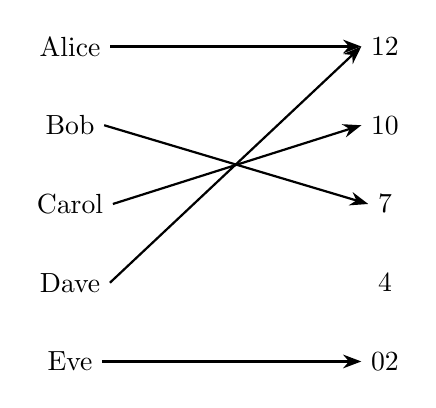
\begin{tikzpicture}[>=Stealth] % Stealth is a nice arrow style
        % Left column of names
        \node (A1) at (0,0) {Alice};
        \node (A2) at (0,-1) {Bob};
        \node (A3) at (0,-2) {Carol};
        \node (A4) at (0,-3) {Dave};
        \node (A5) at (0,-4) {Eve};
        
        % Right column of numbers
        \node (B1) at (4,0) {$12$};
        \node (B2) at (4,-1) {$10$};
        \node (B3) at (4,-2) {$7$};
        \node (B4) at (4,-3) {$4$};
        \node (B5) at (4,-4) {$02$};
        
        % Connecting lines with arrows
        \draw[->, thick, black] (A1.east) -- (B1.west);
        \draw[->, thick, black] (A2.east) -- (B3.west);
        \draw[->, thick, black] (A3.east) -- (B2.west);
        \draw[->, thick, black] (A4.east) -- (B1.west);
        \draw[->, thick, black] (A5.east) -- (B5.west);
    \end{tikzpicture}
    \caption{Example of a function mapping names to numbers.}
    \label{fig:names_to_numbers}
\end{figure}


This assignment of grades, illustrated in \autoref{fig:names_to_numbers}, exemplifies a function.

Functions play a crucial role in mathematics and computer science. They define discrete structures such as sequences and strings and are used to analyse the time complexity of algorithms. Many computer programs are designed to compute values of functions. Recursive functions, defined in terms of themselves, are especially significant in computer science. This section provides an overview of the fundamental concepts of functions needed in the mathematics for software engineering.

\begin{definition}
Let $A$ and $B$ be nonempty sets. A function $f$ from $A$ to $B$ is an assignment of exactly one element of $B$ to each element of $A$. We write $f(a)=b$ if $b$ is the unique element of $B$ assigned by the function $f$ to the element $a$ of $A$. If $f$ is a function from $A$ to $B$, we write $f: A \rightarrow B$.
\end{definition}

\begin{remark}
    Functions are sometimes also called mappings or transformations.
\end{remark}

Functions can be specified in various ways. Sometimes, we explicitly state the assignments, as shown in \autoref{fig:names_to_numbers}. Often, a formula such as \(f(x) = x + 1\) is used to define a function. In other cases, a computer program may specify the function.

\begin{definition}
If $f$ is a function from $A$ to $B$, we say that $A$ is the \textbf{domain} of $f$ and $B$ is the \textbf{co-domain} of $f$. If $f(a)=b$, we say that $b$ is the \textbf{image} of $a$ and $a$ is a \textbf{preimage} of $b$. The \textbf{range}, or image, of $f$ is the set of all images of elements of $A$. Also, if $f$ is a function from $A$ to $B$, we say that $f$ \textbf{maps} $A$ to $B$.    
\end{definition}

When defining a function, we specify its domain, co-domain, and the mapping of elements from the domain to the co-domain. Two functions are equal if they have the same domain, the same co-domain, and map each element of their domain to the same element in the co-domain. 

It's important to note that altering the domain or co-domain results in a different function. Similarly, changing the mapping of elements also produces a different function.


\begin{figure}[htbp]
\centering
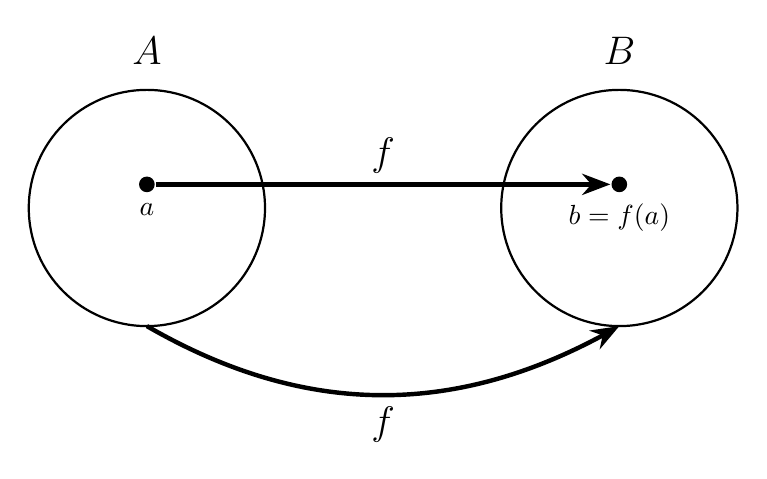
\begin{tikzpicture}[>=Stealth, node distance=4cm, thick, scale=1]

    % Draw larger circles for sets A and B
    \draw[thick] (0,0) circle [radius=1.5cm] node at (0, 2) {\Large $A$};
    \draw[thick] (6,0) circle [radius=1.5cm] node at (6, 2) {\Large $B$};

    % Place larger nodes for elements a and b=f(a)
    \node[fill, circle, inner sep=2pt, label=below:{$a$}] (a) at (0,0.3) {};
    \node[fill, circle, inner sep=2pt, label=below:{$b=f(a)$}] (b) at (6,0.3) {};

    % Draw the larger straight arrow representing f
    \draw[->, ultra thick, black] (a) -- (b) node[midway, above] {\Large $f$};

    % Draw the curved arrow representing f at the bottom, touching the circles
    \draw[->, ultra thick, black, bend right=30] ([shift={(270:1.5cm)}]0,0) 
    to node[midway, below] {\Large $f$} 
    ([shift={(270:1.5cm)}]6,0);

\end{tikzpicture}
\caption{A function \(f\) mapping an element \(a\) from set \(A\) to an element \(b=f(a)\) in set \(B\).}
\label{fig:function_mapping}
\end{figure}

The following examples illustrate various functions. In each example, we describe the domain, co-domain, range, and the assignment of values to the elements of the domain.

\begin{example} What are the domain, co-domain, and range of the function that assigns grades to students described in the first paragraph of the introduction of this section?

\begin{solution}
    Let $G$ be the function that assigns a grade to a student in our Software engineering mathematics class. Note that $G$(Alice) $=12$, for instance. The domain of $G$ is the set \{Alice, Bob, Carol, David, Eve $\}$, and the co-domain is the set $\{12, 10, 7, 4, 02\}$. The range of $G$ is the set $\{12, 10, 7, 02\}$, because each grade except $4$ is assigned to some student.
\end{solution}
    
\end{example}

\begin{example}
    Let $f$ be the function that assigns the last two bits of a bit string of length 2 or greater to that string. For example, $f(11010)=10$. Then, the domain of $f$ is the set of all bit strings of length 2 or greater, and both the co-domain and range are the set $\{00,01,10,11\}$.
\end{example}

\begin{example}
    Let $f: \mathbb{Z} \rightarrow \mathbb{Z}$ assign the square of an integer to this integer. Then, $f(x)=x^2$, where the domain of $f$ is the set of all integers, the co-domain of $f$ is the set of all integers, and the range of $f$ is the set of all integers that are perfect squares, namely, $\{0,1,4,9, \ldots\}$.
\end{example}

\subsection*{One-to-One and Onto Functions}
In mathematics, functions are a fundamental concept used to describe the relationship between two sets. However, not all functions behave the same way. To understand these differences, we introduce the concepts of one-to-one (injective) and onto (surjective) functions.

Some functions never assign the same value to two different domain elements. These functions are said to be \textbf{one-to-one}.

\begin{definition} {One-to-One functions (Injective)}
A function \( f: A \rightarrow B \) is called \textbf{one-to-one} (or \textbf{injective}) if different elements in \( A \) map to different elements in \( B \). In other words, if \( f(a_1) = f(a_2) \), then \( a_1 = a_2 \). This property ensures that no two distinct elements in \( A \) are mapped to the same element in \( B \).     
\end{definition}

Graphically, a function is one-to-one if no horizontal line intersects the graph of the function at more than one point.

\begin{definition}{Onto Functions (Surjective)}
A function \( f: A \rightarrow B \) is called \textbf{onto} (or \textbf{surjective}) if every element in \( B \) is the image of at least one element in \( A \). In other words, for every \( b \in B \), there exists at least one \( a \in A \) such that \( f(a) = b \). This property ensures that the function ``covers'' the entire set \( B \).
\end{definition}

\subsection*{Inverse Functions}

Now, consider a function \( f: A \rightarrow B \) that is both one-to-one and onto. Because \( f \) is onto, every element of \( B \) is the image of some element in \( A \). Furthermore, because \( f \) is one-to-one, every element of \( B \) is the image of a unique element of \( A \). This unique correspondence allows us to define a new function from \( B \) to \( A \) that ``reverses'' the mapping given by \( f \).

\begin{figure}[htbp]
\centering
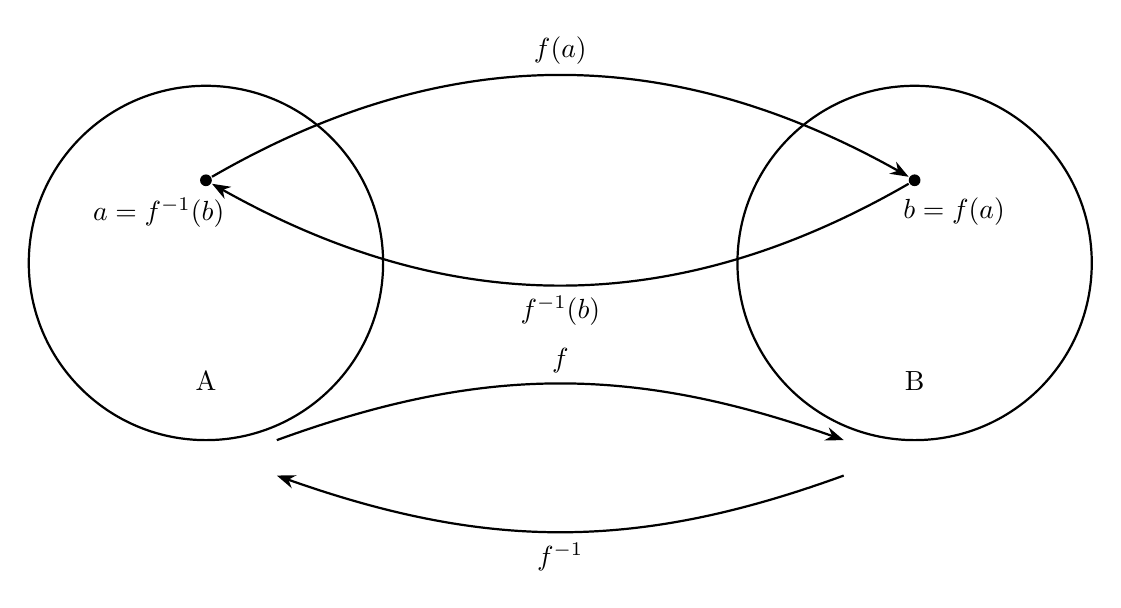
\begin{tikzpicture}[>=Stealth, thick, scale = 1.5]

% Draw circles representing sets A and B
\draw (0,0) circle (1.5cm);
\draw (6,0) circle (1.5cm);

% Labels for sets A and B
\node at (0,-1) {A};
\node at (6,-1) {B};


% Points in sets with adjusted labels
\node[fill=black, circle, inner sep=1.5pt, label={[xshift=-0.6cm]below:{$a = f^{-1}(b)$}}] (A1) at (0,0.7) {};
\node[fill=black, circle, inner sep=1.5pt, label={[xshift=0.5cm]below:{$b = f(a)$}}] (B1) at (6,0.7) {};


% Arrows for f and f^{-1}
\draw[->] (A1) to[bend left=30] node[midway, above] {$f(a)$} (B1);
\draw[->] (B1) to[bend left=30] node[midway, below] {$f^{-1}(b)$} (A1);

% Arrows for f and f^{-1} below the main circles
\draw[->] (0.6,-1.5) to[bend left=20] node[midway, above] {$f$} (5.4,-1.5);
\draw[->] (5.4,-1.8) to[bend left=20] node[midway, below] {$f^{-1}$} (0.6,-1.8);

\end{tikzpicture}
\caption{The function $f^{-1}$ is the inverse of function $f$.}
\label{fig:inv}
\end{figure}

This new function is called the \textbf{inverse function} of \( f \), denoted by \( f^{-1}: B \rightarrow A \). The inverse function \( f^{-1} \) satisfies the following properties:

\[
f(f^{-1}(b)) = b \quad \text{for every } b \in B.
\]
\[
f^{-1}(f(a)) = a \quad \text{for every } a \in A.
\]

We can summarise these considerations in the following definition

\begin{definition}{Inverse Functions}
Let $f$ be a one-to-one correspondence from the set $A$ to the set $B$. The inverse function of $f$ is the function that assigns to an element $b$ belonging to $B$ the unique element $a$ in $A$ such that $f(a)=b$. The inverse function of $f$ is denoted by $f^{-1}$. Hence, $f^{-1}(b)=a$ when $f(a)=b$.    
\end{definition}

These properties show that \( f^{-1} \) effectively undoes the work of \( f \), mapping each element of \( B \) back to the corresponding element in \( A \).

\begin{example}


Let \( f: \mathbb{R} \rightarrow \mathbb{R} \) be defined by \( f(x) = 2x + 3 \). We can check that \( f \) is both one-to-one and onto:

\begin{itemize}
    \item \textbf{One-to-One}: If \( f(x_1) = f(x_2) \), then \( 2x_1 + 3 = 2x_2 + 3 \). Subtracting 3 from both sides gives \( 2x_1 = 2x_2 \), and dividing by 2 yields \( x_1 = x_2 \). Thus, \( f \) is one-to-one.
    \item \textbf{Onto}: Given any \( y \in \mathbb{R} \), we can solve \( y = 2x + 3 \) for \( x \) to find \( x = \frac{y - 3}{2} \). Since this \( x \) exists for every \( y \), \( f \) is onto.
\end{itemize}

Since \( f \) is both one-to-one and onto, it has an inverse function \( f^{-1} \) defined by

\[
f^{-1}(y) = \frac{y - 3}{2}.
\]

  
\end{example}

\subsection*{Composite Functions}
In mathematics, functions can be combined to form new functions. One important way of combining functions is through the composition of functions. The composite of two functions is essentially applying one function to the results of another.

\begin{figure}[htbp]
\centering
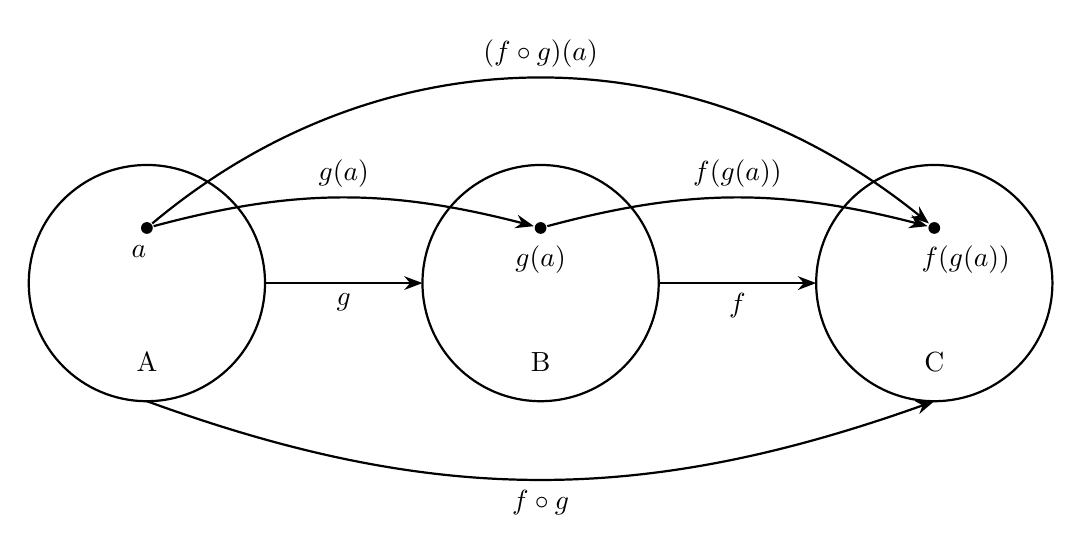
\begin{tikzpicture}[>=Stealth, thick]

% Draw circles representing sets A, B, and C
\draw (0,0) circle (1.5cm);  % Set A
\draw (5,0) circle (1.5cm);  % Set B
\draw (10,0) circle (1.5cm); % Set C

% Labels for sets A, B, and C
\node at (0,-1) {A};
\node at (5,-1) {B};
\node at (10,-1) {C};

% Points in sets with adjusted labels
\node[fill=black, circle, inner sep=1.5pt, label={[xshift=-0.1cm]below:{$a$}}] (A) at (0,0.7) {};

\node[fill=black, circle, inner sep=1.5pt, label=below:{$g(a)$}] (B) at (5,0.7) {};
\node[fill=black, circle, inner sep=1.5pt, label={[xshift=0.4cm]below:{$f(g(a))$}}] (C) at (10,0.7) {};

% Arrows for g and f
\draw[->] (A) to[bend left=15] node[midway, above] {$g(a)$} (B);
\draw[->] (B) to[bend left=15] node[midway, above] {$f(g(a))$} (C);
\draw[->] ([shift={(360:1.5cm)}]0,0) to node[midway, below] {$g$} (3.5,0);
\draw[->] ([shift={(360:0cm)}]6.5,0) to node[midway, below] {$f$} (8.5,0);

% Arrows for f ∘ g and (f ∘ g)(a)
\draw[->] (A) to[bend left=40] node[midway, above] {$(f \circ g)(a)$} (C);
% Draw the curved arrow representing f at the bottom, touching the circles
\draw[->, bend right=20] ([shift={(270:1.5cm)}]0,0) to node[midway, below] {$f \circ g$} ([shift={(270:1.5cm)}]10,0);

\end{tikzpicture}
\caption{The composition of $f$ and $g$.}
\label{fig:composite}
\end{figure}

\begin{definition}
    

Let \( f: B \rightarrow C \) and \( g: A \rightarrow B \) be two functions. The \textbf{composite function} of \( f \) and \( g \), denoted by \( f \circ g \), is a function from \( A \) to \( C \) defined by

\[
(f \circ g)(x) = f(g(x)),
\]

for every \( x \in A \).

\end{definition}

In other words, the composite function \( f \circ g \) means that you first apply the function \( g \) to the input \( x \), and then apply the function \( f \) to the result of \( g(x) \). In \autoref{fig:composite} the composition of functions is shown.

\begin{example}
    

Consider the functions \( f(x) = 2x + 3 \) and \( g(x) = x^2 \). The composite function \( f \circ g \) is given by:

\[
(f \circ g)(x) = f(g(x)) = f(x^2) = 2x^2 + 3.
\]

Here, the function \( g(x) \) squares the input \( x \), and then the function \( f(x) \) multiplies the result by 2 and adds 3.
\end{example}

Now, let's reverse the composition and compute \( g \circ f \):

\[
(g \circ f)(x) = g(f(x)) = g(2x + 3) = (2x + 3)^2.
\]

Notice that \( f \circ g \) and \( g \circ f \) are generally different functions, illustrating that the composition of functions is not commutative.

\begin{example}
    Let $g$ be the function from the set $\{a, b, c\}$ to itself such that $g(a)=b, g(b)=c$, and $g(c)=a$. Let $f$ be the function from the set $\{a, b, c\}$ to the set $\{1,2,3\}$ such that $f(a)=3, f(b)=2$, and $f(c)=1$. What is the composition of $f$ and $g$, and what is the composition of $g$ and $f$ ?

    \begin{solution}
        The composition $f \circ g$ is defined by $(f \circ g)(a)=f(g(a))=f(b)=2$, $(f \circ g)(b)=f(g(b))=f(c)=1$, and $(f \circ g)(c)=f(g(c))=f(a)=3$.
        
        Note that $g \circ f$ is not defined, because the range of $f$ is not a subset of the domain of $g$.
    \end{solution}
\end{example}


\begin{example}{label:}
Let $f$ and $g$ be the functions from the set of integers to the set of integers defined by $f(x)=2 x+3$ and $g(x)=3 x+2$. What is the composition of $f$ and $g$ ? What is the composition of $g$ and $f$?

\begin{solution}
Both the compositions $f \circ g$ and $g \circ f$ are defined. Moreover,
\[
(f \circ g)(x)=f(g(x))=f(3 x+2)=2(3 x+2)+3=6 x+7
\]
and
\[
(g \circ f)(x)=g(f(x))=g(2 x+3)=3(2 x+3)+2=6 x+11 .
\]
\end{solution}
\end{example}

\begin{remark}
Even though \( f \circ g \) and \( g \circ f \) are defined for the functions \( f \) and \( g \) in example 35, \( f \circ g \) and \( g \circ f \) are not equal. In other words, the commutative law does not hold for the composition of functions.
  
\end{remark}

When the composition of a function and its inverse is formed, in either order, an identity function is obtained. To see this, suppose that \( f \) is a one-to-one correspondence from the set \( A \) to the set \( B \). Then the inverse function \( f^{-1} \) exists and is a one-to-one correspondence from \( B \) to \( A \). The inverse function reverses the correspondence of the original function, so \( f^{-1}(b)=a \) when \( f(a)=b \), and \( f(a)=b \) when \( f^{-1}(b)=a \).

Hence,

\[
\left(f^{-1} \circ f\right)(a) = f^{-1}(f(a)) = f^{-1}(b) = a,
\]

and

\[
\left(f \circ f^{-1}\right)(b) = f\left(f^{-1}(b)\right) = f(a) = b.
\]

Consequently, \( f^{-1} \circ f = I_A \) and \( f \circ f^{-1} = I_B \), where \( I_A \) and \( I_B \) are the identity functions on the sets \( A \) and \( B \), respectively. That is, \( \left(f^{-1}\right)^{-1} = f \).

\begin{example}
    If $f: \mathbb{R} \rightarrow \mathbb{R}$ is defined as $f(x)=2 x+3$, then $f^{-1}(x)=\frac{x-3}{2}$. The composition $f \circ f^{-1}$ would be the identity function $I_{\mathbb{R}}$ on the real numbers, meaning $f\left(f^{-1}(x)\right)=x$ for all $x \in \mathbb{R}$.
\end{example}

\section{Graphical Identification of Function Types}
Understanding the behaviour of different types of functions is fundamental in mathematics. Functions can be classified based on their graphical patterns, which provide valuable insights into their characteristics. In this section, we will explore various types of functions, including linear, quadratic, exponential, and more. By examining their graphs, we can identify key features such as intercepts, slopes, curvature, and asymptotic behaviour, enabling us to distinguish between these different types of functions effectively.

\subsection*{Linear Functions}
The general equation for a linear function is given by

\[
y = ax + b \quad \text{(often written as } y = mx + b\text{)},
\]

where \(a\) (or \(m\)) represents the slope and \(b\) is the y-intercept. The domain of this function is all real numbers. This equation is in slope-intercept form because \(a\) (or \(m\)) gives the slope and \(b\) gives the y-intercept. If \(a = 0\), the function simplifies to \(y = b\), which is a constant function.

The parent function for a linear equation is

\[
y = x.
\]

The transformed function can be written in the point-slope form as

\[
y = y_1 + a(x - x_1),
\]

where the graph contains the point \((x_1, y_1)\) and has slope \(a\). In this form:
\begin{itemize}
    \item \(a\) is the vertical dilation (slope),
    \item \(y_1\) represents the vertical translation,
    \item \(x_1\) represents the horizontal translation.
\end{itemize}

This point-slope form can also be written as

\[
y - y_1 = a(x - x_1),
\]

where the coordinates of the fixed point \((x_1, y_1)\) appear with a negative sign. The form \(y = y_1 + a(x - x_1)\) expresses \(y\) explicitly in terms of \(x\), making it easier to enter into a graphing calculator.

\begin{figure}[htbp]
    \centering
    \includegraphics[width=1\textwidth]{figure/book1.png} % Adjust width here to scale the image
    \caption{Linear functions}
    \label{fig:book_image}
\end{figure}

The graph of a linear function is a straight line. The parent function \(y = x\) is shown on the left in \autoref{fig:book_image}, the slope-intercept form in the middle, and the point-slope form on the right.

For the slope-intercept form: "Start at \(b\) on the \(y\)-axis, move \(x\) units horizontally, and rise \(ax\) units vertically." For the point-slope form: "Start at \((x_1, y_1)\), move \((x - x_1)\) units horizontally, and rise \(a(x - x_1)\) units vertically."

\subsection*{Quadratic Functions}
The general equation for a quadratic function is given by

\[
y = ax^2 + bx + c,
\]

where \(a \neq 0\), and \(a\), \(b\), and \(c\) are constants. The domain of this function is all real numbers.

\begin{figure}[htbp]
    \centering
    \includegraphics[width=1\textwidth]{figure/book2.png} % Adjust width here to scale the image
    \caption{Quadratic functions}
    \label{fig:book_image2}
\end{figure}

The parent function for a quadratic equation is

\[
y = x^2,
\]

where the vertex of the parabola is at the origin \((0, 0)\).

The transformed function can be written in vertex form as

\[
y = k + a(x-h)^2,
\]

where the vertex of the parabola is located at \((h, k)\). In this form:
\begin{itemize}
    \item \(k\) represents the vertical translation,
    \item \(h\) represents the horizontal translation,
    \item \(a\) represents the vertical dilation.
\end{itemize}

Vertex form can also be written as

\[
y - k = a(x-h)^2,
\]

but expressing \(y\) explicitly in terms of \(x\) makes the equation easier to enter into a graphing calculator.

The graph of a quadratic function is a parabola (from the Greek word for "along the path of a ball"). The parabola is concave up if \(a > 0\) and concave down if \(a < 0\). This behaviour is illustrated in \autoref{fig:book_image2}.

\subsection*{Power Functions}
The general equation for a power function is given by

\[
y = ax^b,
\]

where \(a\) and \(b\) are nonzero constants. The domain of the function depends on the value of \(b\):
\begin{itemize}
    \item If \(b > 0\), the domain is all real numbers.
    \item If \(b < 0\), the domain excludes \(x = 0\) to avoid division by zero.
    \item If \(b\) is not an integer, the domain usually excludes negative numbers to avoid taking roots of negative numbers.
\end{itemize}
In most applications, the domain is restricted to non-negative numbers.

\begin{figure}[htbp]
    \centering
    \includegraphics[width=1\textwidth]{figure/book3.png} % Adjust width here to scale the image
    \caption{Power functions}
    \label{fig:book_image3}
\end{figure}

The parent function for a power function is

\[
y = x^b.
\]

For the general power function \(y = ax^b\):
\begin{itemize}
    \item If \(b > 0\), then \(y\) varies directly with the \(b\)th power of \(x\), meaning \(y\) is directly proportional to the \(b\)th power of \(x\).
    \item If \(b < 0\), then \(y\) varies inversely with the \(b\)th power of \(x\), meaning \(y\) is inversely proportional to the \(b\)th power of \(x\).
\end{itemize}

The dilation factor \(a\) serves as the proportionality constant.

The translated form of a power function is

\[
y = d + a(x - c)^b,
\]

where \(c\) and \(d\) are the horizontal and vertical translations, respectively. This can be compared with the translated forms of linear and quadratic functions:

\[
\begin{aligned}
& y = y_1 + a(x - x_1) &\text{(linear function)}, \\
& y = k + a(x - h)^2 &\text{(quadratic function)}.
\end{aligned}
\]

Unless otherwise stated, "power function" will imply the untranslated form, \(y = ax^b\).

\autoref{fig:book_image3} shows the graphs of power functions for different values of \(b\). In all cases, \(a > 0\). The shape and concavity of the graph depend on the value of \(b\):
\begin{itemize}
    \item If \(b > 0\), the graph contains the origin.
    \item If \(b < 0\), the graph has the axes as asymptotes.
    \item The function is increasing if \(b > 0\) and decreasing if \(b < 0\).
    \item The graph is concave up if \(b > 1\) or \(b < 0\), and concave down if \(0 < b < 1\).
\end{itemize}
The concavity of the graph describes the rate at which \(y\) increases. For \(b > 0\), concave up indicates that \(y\) is increasing at an increasing rate, while concave down indicates that \(y\) is increasing at a decreasing rate.

\subsection*{Exponential Functions}

The general equation for an exponential function is given by

\[
y = a b^x,
\]

where \(a\) and \(b\) are constants, \(a \neq 0\), \(b > 0\), and \(b \neq 1\). The domain of this function is all real numbers.

The parent function for an exponential equation is

\[
y = b^x,
\]
where the asymptote is the \(x\)-axis.

\begin{figure}[htbp]
    \centering
    \includegraphics[width=1\textwidth]{figure/book4.png} % Adjust width here to scale the image
    \caption{Exponential functions}
    \label{fig:book_image4}
\end{figure}

In the equation \(y = a b^x\), we say that "\(y\) varies exponentially with \(x\)." This means that \(y\) changes by a constant factor \(b\) for each unit increase in \(x\).

The translated form of the exponential function is

\[
y = a b^x + c,
\]

where the asymptote is the line \(y = c\). Unless otherwise stated, "exponential function" will refer to the untranslated form \(y = a b^x\).

\autoref{fig:book_image4} illustrates exponential functions for different values of \(a\) and \(b\). The key properties of the graph are as follows:
\begin{itemize}
    \item The constant \(a\) is the \(y\)-intercept of the graph.
    \item The function is increasing if \(b > 1\) and decreasing if \(0 < b < 1\), provided \(a > 0\).
    \item If \(a < 0\), the function's behavior is reversed: it is decreasing if \(b > 1\) and increasing if \(0 < b < 1\).
    \item The graph is concave up if \(a > 0\) and concave down if \(a < 0\).
\end{itemize}

Mathematicians often use one of two particular constants as the base for an exponential function: either 10, which is the base of the decimal system, or the naturally occurring number \( e \), which approximately equals 2.71828. These bases are significant in various mathematical applications.

\begin{definition}{Special Exponential Functions}

\begin{align*}
y &= a \cdot 10^{bx} \hspace{1cm} \text{base-10 exponential function} \\
y &= a \cdot e^{bx}  \hspace{1.2cm} \text{natural (base-}e\text{) exponential function,}
\end{align*}

where $a$ and $b$ are constants and the domain is all real numbers.
    
\end{definition}

To generalise the exponential function, the variable in the exponent is often multiplied by a constant. The (untranslated) general forms of these exponential functions are given below:

\[
y = a \cdot 10^{bx}
\quad \text{and} \quad
y = a \cdot e^{bx}
\]

These functions can be further generalised by incorporating translations in both the \(x\)- and \(y\)-directions. The translated forms are:

\[
y = a \cdot 10^{b(x - c)} + d
\quad \text{and} \quad
y = a \cdot e^{b(x - c)} + d
\]

The base-\(e\) exponential function, in particular, has a significant advantage when studying calculus, as the rate of change of \(e^x\) is equal to \(e^x\) itself.

\section{Logarithms}
Any positive number can be written as a power of 10. For instance,

\[
\begin{aligned}
3 & = 10^{0.477 \ldots} \\
5 & = 10^{0.6989 \ldots} \\
15 & = 10^{1.1760 \ldots}
\end{aligned}
\]

The exponents \(0.4771 \ldots\), \(0.6989 \ldots\), and \(1.1760 \ldots\) are called the base-10 logarithms of 3, 5, and 15, respectively:

\[
\begin{aligned}
\log 3 & = 0.4771 \ldots \\
\log 5 & = 0.6989 \ldots \\
\log 15 & = 1.1760 \ldots
\end{aligned}
\]

To better understand the meaning of logarithms, press \texttt{LOG} 3 on your calculator. You will get:

\[
\log 3 = 0.477121254 \ldots
\]

Then, without rounding, raise 10 to this power. You will obtain:

\[
10^{0.477121254 \ldots} = 3
\]

The powers of 10 have the normal properties of exponentiation. For instance,
\[
\begin{aligned}
15 & = (3)(5) = \left(10^{0.4771 \ldots}\right)\left(10^{0.6999 \ldots}\right) \\
& = 10^{0.4771 \ldots + 0.6599 \ldots} \\
& = 10^{1.1760 \ldots}
\end{aligned}
\]

This means \(10^{0.4771 \ldots + 0.6599 \ldots} = 10^{1.1760 \ldots}\). Here, you add the exponents while keeping the same base. You can verify with your calculator that \(10^{1.1760 \ldots}\) indeed equals 15.

From this example, you can infer that logarithms have the same properties as exponents. This is expected because logarithms \textit{are} exponents. For instance,

\[
\log(3 \cdot 5) = \log 3 + \log 5 \quad \text{\textit{The logarithm of a product equals the sum of the logarithms of the factors}.}
\]

From the values given earlier, you can also show that:

\[
\log \frac{15}{3} = \log 15 - \log 3 \quad \text{\textit{The logarithm of a quotient}.}
\]

This property is reasonable because you divide powers of equal bases by subtracting the exponents:

\[
\frac{15}{3} = \frac{10^{1.1760 \ldots}}{10^{0.477 \ldots}} = 10^{1.1760 \ldots - 0.4771 \ldots} = 10^{0.6989 \ldots} = 5
\]

Since a power can be written as a product, you can find the logarithm of a power as follows:

\[
\begin{aligned}
\log 34 & = \log (3 \cdot 3 \cdot 3 \cdot 3) = \log 3 + \log 3 + \log 3 + \log 3 \\
& = 4 \log 3 \quad \text{\textit{Combine like terms}.}
\end{aligned}
\]

The logarithm of a power equals the exponent of that power times the logarithm of the base. To verify this result, observe that \(3^4 = 81\). Press \(4 \times \texttt{LOG}\,3\) on your calculator, and you'll find it equals \(1.9084 \ldots\).

\begin{definition}{Base-10 Logarithms}

\[
\log x=y \iff 10^y=x
\]

\textit{Verbally}: $\log x$ is the exponent in the power of 10 that gives $x$   
\end{definition}

The term logarithm comes from the Greek words \emph{logos}, meaning "ratio," and \emph{arithmos}, meaning "number." Before the invention of calculators, base-10 logarithms were calculated approximately using infinite series and recorded in tables. Products involving many factors, such as
\[
(357)(4.367)(22.4)(3.142)
\]
could be calculated by adding their logarithms (exponents) rather than tediously multiplying several pairs of numbers. This method was invented by Englishman Henry Briggs (1561–1630) and Scotsman John Napier (1550–1616). The name logarithm, thus, reflects this "logical way to do arithmetic".

\begin{custombox}{Properties of base-10 logarithms}
\begin{itemize}
    \item Log of a Product:
    
    \[
    \log x y=\log x+\log y
    \]
    
    \textit{Verbally}: The $\log$ of a product equals the sum of the logs of the factors.
    \vspace{0.2cm}
    \item Log of a Quotient:
    
    \[
    \log \frac{x}{y}=\log x-\log y
    \]
    \vspace{0.1cm}
    \textit{Verbally}: The $\log$ of a quotient equals the log of the numerator minus the $\log$ of the denominator.
    \vspace{0.2cm}
    \item Log of a Power:
    \[
    \log x^y=y \log x
    \]
    \textit{Verbally}: The $\log$ of a power equals the exponent times the log of the base.
\end{itemize}

   
\end{custombox}

\begin{example} Find $x$ if $\log_{10} 10^{3.721}=x$

\begin{solution}
By definition, the logarithm is the exponent of 10. So $x=3.721$.
\end{solution}
\end{example}

\begin{example} Find $x$ if $0.258=10^x$

\begin{solution}
   By definition, $x$, the exponent of 10 , is the logarithm of 0.258 .

    \[
    x=\log_{10} 0.258=-0.5883 \ldots
    \]
\end{solution}
    
\end{example}

\begin{custombox}{The most important thing to remember about logarithms is this}
    \textbf{A logarithm is an exponent.}
\end{custombox}

\subsection*{Logarithms with Any Base: The Change-of-Base Property}
If \(x = 10^y\), then \(y\) is the base-10 logarithm of \(x\). Similarly, if \(x = 2^y\), then \(y\) is the base-2 logarithm of \(x\). The only difference between these logarithms is the number that serves as the base. To distinguish among logarithms with different bases, the base is written as a subscript after the abbreviation "log." For instance:

\[
\begin{aligned}
3 &= \log_2 8 \Leftrightarrow 2^3 = 8, \\
4 &= \log_3 81 \Leftrightarrow 3^4 = 81, \\
2 &= \log_{10} 100 \Leftrightarrow 10^2 = 100.
\end{aligned}
\]

The symbol \(\log_2 8\) is pronounced "log to the base 2 of 8." The symbol \(\log_{10} 100\) is, of course, equivalent to \(\log 100\), as defined in the previous section. Note that in all cases, a logarithm represents an exponent.

\begin{definition}{Logarithm with Any Base}
\textit{Algebraically}:

\hspace{1cm}$\log _b x=y$ if and only if $b^y=x, \quad$ where $b>0, b \neq 1$, and $x>0$

\vspace{0.3cm}

\textit{Verbally}:

\hspace{1cm} $\log _b x=y$ means that $y$ is the exponent of $b$ that gives $x$ as the answer.
    
\end{definition}

The way you pronounce the symbol for logarithm gives you a way to remember the definition. The next two examples show you how to do this.

\begin{example} Write $\log _5 c=a$ in exponential form.

\begin{solution}

Think this:
\begin{itemize}
    \item "\(\log_5 \ldots\)" is read as "log base 5 \(\ldots\)," meaning 5 is the base.
    \item A logarithm is an exponent. Since the \(\log\) equals \(a\), \(a\) must be the exponent.
    \item The "answer" obtained from \(5^a\) is the argument of the logarithm, denoted as \(c\).
\end{itemize}

Write only this: 

\[
5^a = c
\]
\end{solution}
\end{example}

\begin{example} Write $z^4=m$ in logarithmic form.

\begin{solution}
    $\log _z m=4$
\end{solution}
    
\end{example}

Two bases of logarithms are used frequently enough to have their own key on most calculators. One is the base-10 logarithm, also known as the common logarithm, as discussed in the previous section. The other is the base-\(e\) logarithm, known as the natural logarithm, where \(e = 2.71828 \ldots\), a naturally occurring number (like \(\pi\)) that will be advantageous in your future mathematical studies.

The symbol \(\ln x\) (pronounced "el en of \(x\)") is used for natural logarithms, and is defined as:
\[
\ln x = \log_e x
\]

\begin{definition}{Common Logarithm and Natural Logarithm}
\hspace{1cm} \textit{Common}: The symbol $\log x$ means $\log _{10} x$.

\hspace{1cm}  \textit{Natural}: \hspace{0.2cm}The symbol $\ln x$ means $\log _e x$, where $e$ is a constant equal to $2.71828182845 \ldots$
\end{definition}

\begin{example} Find $\log _5 17$. Check your answer by an appropriate numerical method.

\begin{solution} Let $x=\log _5 17$.

\begin{equation*}
\begin{aligned}
& 5^x=17 \\
& \log _{10} 5^x=\log _{10} 17 \\
& x \log _{10} 5=\log _{10} 17 \\
& x=\frac{\log _{10} 17}{\log _{10} 5}=1.7603 \ldots \\
& \log _5 17=1.7603 \ldots \\
& 5^{1.7603 \ldots}=17
\end{aligned}
\end{equation*}
\end{solution}
\end{example}

In this example, note that the base-5 logarithm of a number is directly proportional to the base-10 logarithm of that number. The conclusion of the example can be expressed as follows:

\[
\log_5 17 = \frac{1}{\log_{10} 5} \cdot \log_{10} 17 = 1.4306 \ldots \log_{10} 17
\]

To find the base-5 logarithm of any number, simply multiply its base-10 logarithm by \(1.4306 \ldots\) (that is, divide by \(\log_{10} 5\)).

This proportional relationship is known as the change-of-base property. From the results of Example 3, you can write:

\[
\log_5 17 = \frac{\log_{10} 17}{\log_{10} 5}
\]

Notice that the logarithm with the desired base is isolated on the left side of the equation, while the two logarithms on the right side share the same base—typically one that is available on your calculator. The box below illustrates this property for bases \(a\) and \(b\) with argument \(x\):

\begin{custombox}{The Change-of-Base Property of Logarithms}

\begin{equation*}
\log _a x=\frac{\log _b x}{\log _b a} \quad \text { or } \quad \log _a x=\frac{1}{\log _b a}\left(\log _b x\right)
\end{equation*}
    
\end{custombox}

\begin{example}
Find $\ln 29$ using the change-of-base property with base-10 logarithms. Check your answer directly by pressing $\ln 29$ on your calculator.

\begin{solution}

\[
\ln 29=\frac{\log 29}{\log e}=\frac{1.4623 \ldots}{0.4342 \ldots}=3.3672 \ldots
\]

\hspace{0.9cm} Directly: $\quad \ln 29=3.3672 \ldots,$

which agrees with the answer we got using the change-of-base property.
\end{solution}
\end{example}

\begin{custombox}{Properties of Logarithms}
\setlength{\leftskip}{1cm}  % Reset the text indent
\setlength{\rightskip}{1cm} % Reset the right indent
The Logarithm of a Power:
$$
\log _b x^y=y \log _b x
$$

\textit{Verbally}: The logarithm of a power equals the product of the exponent and the logarithm of the base.
\vspace{0.5cm}
The Logarithm of a Product:
$$
\log _b(x y)=\log _b x+\log _b y
$$
\textit{Verbally}: The logarithm of a product equals the sum of the logarithms of the factors.
\vspace{0.5cm}
The Logarithm of a Quotient:
$$
\log _b \frac{x}{y}=\log _b x-\log _b y
$$

\textit{Verbally}: The logarithm of a quotient equals the logarithm of the numerator minus the logarithm of the denominator.

\setlength{\leftskip}{0cm}  % Reset the text indent
\setlength{\rightskip}{0cm} % Reset the right indent

\end{custombox}

\subsection*{Solving Exponential and Logarithmic Equations}
Logarithms provide a way to solve an equation with a variable in the exponent or to solve an equation that already contains logarithms. We will demonstrate this through the next few examples.

\begin{example} Solve the exponential equation $7^{3 x}=983$ algebraically, using logarithms.

\begin{solution}
\begin{align*}
& 7^{3x} = 983  \\
& \log 7^{3x} = \log 983 && \texttt{\small Take the base-10 logarithm of both sides.} \\
& 3x \log 7 = \log 983 && \texttt{\small Apply the logarithm power property.} \\
& x = \frac{\log 983}{3 \log 7} && \texttt{\small Divide both sides by the coefficient of x.}\\
& x = 1.1803 \ldots   
\end{align*}


\end{solution}
    
\end{example}

\begin{example} Solve the equation
    \begin{equation*}
\log _2(x-1)+\log _2(x-3)=3
\end{equation*}

\newpage

\begin{solution}

\begin{align*}
& \log _2(x-1)+\log _2(x-3)=3  \\
& \log _2[(x-1)(x-3)]=3 && \texttt{\small Apply the logarithm of a product property.} \\
& 2^3=(x-1)(x-3) && \texttt{\small Use the definition of logarithm.} \\
& 8=x^2-4 x+3 && \texttt{\small Expand the product.}\\
& x^2-4 x-5=0 && \texttt{\small Reduce one side to zero. Use the symmetric }\\
&\vspace{-0.2cm}   && \texttt{\small property of equality.} \\
& (x-5)(x+1)=0 && \texttt{\small Solve by factoring.} \\
& x=5 \quad \text{ or } \quad x=-1
\end{align*}
We need to be cautious here because the solutions in the final step are the solutions of the quadratic equation, and we must make sure they are also solutions of the original logarithmic equation. Check by substituting the solutions into the original equation.

\begin{minipage}[t]{0.45\textwidth}
If $x=5$, then
\[
\begin{aligned}
& \log _2(5-1)+\log _2(5-3) \\
& =\log _2 4+\log _2 2 \\
& =2+1=3
\end{aligned}
\]
\end{minipage}%
\hfill
\begin{minipage}[t]{0.45\textwidth}
If $x=-1$, then
\[
\begin{aligned}
& \log _2(-1-1)+\log _2(-1-3) \\
& =\log _2(-2)+\log _2(-4)
\end{aligned}
\]
which is undefined.
\end{minipage}

\end{solution}

\end{example}

\begin{example} Solve the equation

\[
e^{2 x}-3 e^x+2=0
\]

\begin{solution}

\[
\begin{aligned}
& e^{2 x}-3 e^x+2=0 \\
& \left(e^x\right)^2-3 e^x+2=0
\end{aligned}
\]
We realise that this is a quadratic equation in the variable $e^x$. Using the quadratic formula, you get

\[
\begin{aligned}
& e^x=\frac{+3 \pm \sqrt{9-4(2)}}{2}=\frac{3 \pm 1}{2} \\
& e^x=2 \text { or } e^x=1
\end{aligned}
\]


You now have to solve these two equations.
\[
\begin{array}{ll}
e^x=2 & \qquad e^x=1 \\
x=\ln 2=0.6931 \ldots & \qquad x=0
\end{array}
\]
Check:

\[
\begin{array}{ll}
e^{2 \ln 2}-3 e^{\ln 2}+2 & \qquad \left(e^0\right)^2-3 e^0+2 \\
=\left(e^{\ln 2}\right)^2-3 e^{\ln 2}+2 & \qquad =1^2-3(1)+2=0 \\
=2^2-3(2)+2=0 &
\end{array}
\]
Both solutions are correct.
\end{solution}  
\end{example}

\newpage

\begin{example} Solve the logarithmic equation $\ln (x+3)+\ln (x+5)=0$

\begin{solution}
    \[
\begin{aligned}
& \ln (x+3)+\ln (x+5)=0 \\
& \ln [(x+3)(x+5)]=0 \\
& (x+3)(x+5)=e^0=1 \\
& x^2+8 x+15=1 \\
& x^2+8 x+14=0 \\
& x=-2.5857 \ldots \quad \text { or } \qquad x=-5.4142 \ldots
\end{aligned}
\]
Check:
\[
\begin{aligned}
& x=-2.5857 \ldots: \\
& \ln (-2.5857 \ldots+3)+\ln (-2.5857 \ldots+5) \\
& =\ln (0.4142 \ldots)+\ln (2.4142 \ldots) \\
& =-0.8813 \ldots+0.8813 \ldots=0
\end{aligned}
\]
which is ok.

\[
\begin{aligned}
& x=-5.4142 \ldots: \\
& \ln (-5.4142 \ldots+3)+\ln (-5.4142 \ldots+5) \\
& =\ln (-2.4142 \ldots)+\ln (-0.4142 \ldots)
\end{aligned}
\]

which is undefined.

The only valid solution is $x=-2.5857 \ldots$.
\end{solution}
    
\end{example}



\chapter{Number Systems}
\label{chap:ch2}
Numbers are the foundation of mathematics, representing quantities, measurements, and relationships in both abstract and concrete forms. The study of numbers dates back thousands of years, with early civilisations like the Babylonians, Egyptians, and Greeks laying the groundwork for modern number theory. These ancient cultures developed basic arithmetic, including addition, subtraction, multiplication, and division, which are still taught today.

Number theory, often called the "Queen of Mathematics," is a branch of mathematics devoted to the study of integers and the relationships between them. It encompasses a wide range of topics, including prime numbers, divisibility, modular arithmetic, and the properties of number systems. Number theory has a rich history, with significant contributions from mathematicians such as Euclid, who proved the infinitude of prime numbers around 300 BCE, and Pierre de Fermat, known for Fermat's Last Theorem, a problem that puzzled mathematicians for over 350 years until it was finally solved by Andrew Wiles in 1994.

\begin{figure}[htbp]
    \centering
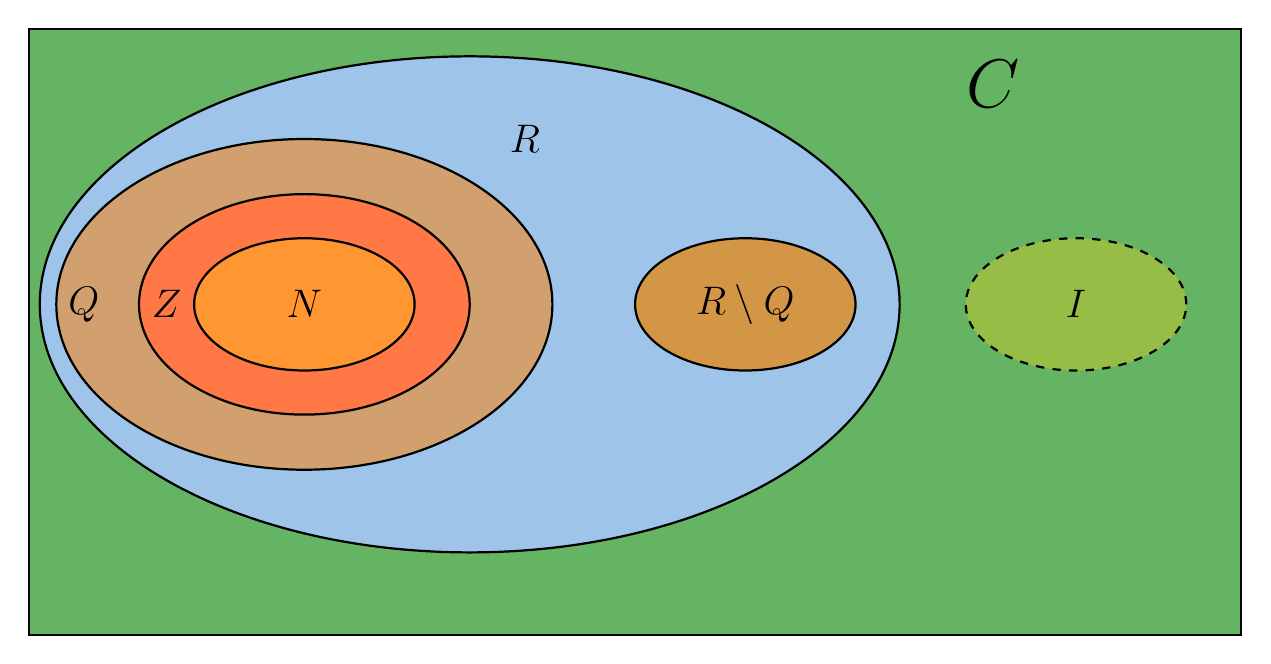
\begin{tikzpicture}[scale=0.7]

    % Complex Numbers (outer square)
    \draw[thick, fill=mseComplex] (-12, -6) rectangle (10, 5);
    \node at (5.5, 4) {\Huge $\mathbb{C}$};
    
    % Real Numbers (largest set)
    \draw[thick, fill=mseReals] (-4,0) ellipse (7.8cm and 4.5cm);
    \node at (-3, 3) {\Large $\mathbb{R}$};
    
    % Rational Numbers
    \draw[thick, fill=mseRationals] (-7,0) ellipse (4.5cm and 3cm);
    \node at (-11, 0) {\Large$\mathbb{Q}$};
    
    % Integers
    \draw[thick, fill=mseIntegers] (-7,0) ellipse (3cm and 2cm);
    \node at (-9.5, 0) {\Large$\mathbb{Z}$};
    
    % Natural Numbers
    \draw[thick, fill=mseNaturals] (-7,0) ellipse (2cm and 1.2cm);
    \node at (-7, 0) {\Large$\mathbb{N}$};
    
    % Irrational Numbers
    \draw[thick, fill=mseIrrationals] (1,0) ellipse (2cm and 1.2cm);
    \node at (1, 0) {\Large$\mathbb{R} \setminus \mathbb{Q} $};
    
    % Imaginary Numbers
    \draw[thick, dashed, fill=mseImaginary] (7,0) ellipse (2cm and 1.2cm);
    \node at (7, 0) {\Large $\mathbb{I}$};

\end{tikzpicture}
    \caption{Venn diagram of numbers}
    \label{fig:venn_num}
\end{figure}

Throughout history, number theory has evolved from a purely theoretical pursuit to a field with practical applications in modern technology. For example, cryptography, the science of securing communication, relies heavily on number theory, particularly the properties of prime numbers and modular arithmetic. The algorithms that protect our online transactions and digital communications are built upon the principles of number theory.

In this chapter, we will explore various aspects of numbers and number theory, starting with the basics of integers, prime numbers, and number systems, and gradually advancing to more complex topics. By understanding the fundamental properties of numbers, we gain insights into the mathematical structures that underpin the digital world and beyond.

\begin{remark}
    \autoref{fig:venn_num} may appear misleading at first glance, as it suggests that there are real numbers which are neither rational nor irrational (depicted by the blue region). However, this is not the case. The set of real numbers is exclusively comprised of rational and irrational numbers. This is precisely why the set of irrational numbers is denoted as \(\mathbb{R} \setminus \mathbb{Q}\), meaning "all real numbers except the rational numbers". The same is true of the complex numbers; the are all composed of the real numbers and the imaginary numbers.
\end{remark}


\begin{table}[ht]
\centering
\caption{Types of Numbers and Their Properties}
\label{tab:number_types}
\renewcommand{\arraystretch}{1.6} % Adjust the row height for the entire table
\begin{tabular}{|m{3.1cm}|>{\centering\arraybackslash}m{1.5cm}|m{5.4cm}|m{5cm}|}
\hline
\raggedright\text{Natural Numbers} & \(\mathbb{N}\) & Numbers used for counting (all positive integers). & \(0, 1, 2, \ldots\) \\ \hline
\raggedright\text{Integers} & \(\mathbb{Z}\) & All positive and negative whole numbers. & \(\{\ldots, -2, -1, 0, 1, 2, \ldots\}\) \\ \hline
\raggedright\text{Rational Numbers} & \(\mathbb{Q}\) & All real numbers which can be expressed as a fraction, \(\frac{p}{q}\), where \(p\) and \(q\) are integers and \(q \neq 0\). All integers are rational numbers as \(1\) is a non-zero integer. & \(\dfrac{1}{5}, \dfrac{5}{1} (=5), \dfrac{2}{3}, \dfrac{3}{2}, \dfrac{0}{3} (=0)\) \\ \hline
\raggedright\text{Irrational Numbers} & \(\mathbb{R}\ \setminus \mathbb{Q}\) & All real numbers which cannot be expressed as a fraction whose numerator and denominator are integers (i.e., all real numbers which aren't rational). & \(\pi, \sqrt{2}, \sqrt{3}\) \\ \hline
\raggedright\text{Real Numbers} & \(\mathbb{R}\) & Includes all numbers on the number line. & \(\dfrac{1}{5}, \sqrt{\dfrac{1}{5}}, 0, -2\) \\ \hline
\raggedright\text{Imaginary Numbers} & \(\mathbb{I}\) & Numbers which are the product of a real number and the imaginary unit \(i\) (where \(i = \sqrt{-1}\)). & \(\begin{array}{l}
\vspace{3pt} 3i = \sqrt{-9},\ -5i = \sqrt{-25}, \\
3\sqrt{2}i = \sqrt{-18} \vspace{3pt}
\end{array}\) \\ \hline
\raggedright\text{Complex Numbers} & \(\mathbb{C}\) & All numbers which can be expressed in the form $a+b i$ where $a$ and $b$ are real numbers and $i=\sqrt{-1}$. Each complex number is a combination of a real number $(a)$ and an imaginary number $(b i)$. & $1+2 i, 1, i,-3 i, 0,-5+i$ \\ \hline
\end{tabular}
\end{table}

\begin{remark}
Many numbers are included in more than one set. \autoref{tab:number_types} offers an overview of the names, properties of and symbols used for the main number types.
\end{remark}

\section{Types of Numbers}
Let's explore the various types of numbers, including natural numbers, whole numbers, integers, rational numbers, irrational numbers, and real numbers - imaginary numbers and complex numbers are left out of this discussion.

\subsection*{Natural Numbers}
We begin with the natural numbers. We distinguish between whole numbers: $0, 1, 2, 3, \ldots$ and counting numbers: $1, 2, 3, \ldots$. These numbers are primarily used for counting. Natural numbers are often regarded as exact values (e.g., there are 4 tires on a car, 8 legs on a spider). However, in some contexts, they may be used as approximations (e.g., there were approximately 1000 people in the crowd).

One of the key properties of natural numbers is that they are \textit{closed} under certain operations, such as addition and multiplication. This means that if you take any two natural numbers and add or multiply them, the result will always be another natural number. For example, if $a$ and $b$ are natural numbers, then both $a + b$ and $a \times b$ are also natural numbers.

There is very little consensus as to whether the symbol $\mathbb{N}$ includes 0. Therefore, the set of whole numbers (that include 0) is often denoted $\mathbb{W}$.

\subsection*{Integers}
Integers are the basic building blocks of number theory, consisting of the set of whole numbers and their negatives. Formally, integers include numbers like $\ldots,-3,-2,-1,0,1,2,3, \ldots$ Basic arithmetic operations, such as addition and multiplication, follow certain properties:

\begin{custombox}{{Commutative, Associative, and Distributive Laws}}


    \begin{itemize}
    \item Commutativity: $a+b=b+a$
    \item Associativity: $(a+b)+c=a+(b+c)$
    \item Distributive property: $a \times(b+c)=a \times b+a \times c$
    \end{itemize}
    
\end{custombox}

Integers are a fundamental set of numbers in mathematics, denoted by the symbol $\mathbb{Z}$. This set includes all the positive and negative whole numbers, as well as zero. Integers extend the natural numbers by incorporating their additive inverses, thereby allowing for the complete operation of subtraction within the set.

\textbf{Additive Identity:} The number \(0\) is known as the additive identity. This is because for any integer \(a\), adding zero does not change the value of \(a\). In mathematical terms, this property is expressed as \(0 + a = a + 0 = a\). This identity is crucial because it ensures that the set of integers remains stable under addition.
    
 \textbf{Multiplicative Identity:} Similarly, the number \(1\) serves as the multiplicative identity. For any integer \(a\), multiplying by one leaves the value of \(a\) unchanged: \(1 \times a = a \times 1 = a\). This property underpins the stability of integers under multiplication, maintaining the integrity of the set.
    
\textbf{Additive Inverse:} For each integer \(a\), there exists a corresponding additive inverse, denoted as \(-a\). The additive inverse is defined such that when \(a\) and \(-a\) are added together, the result is the additive identity, zero: \(a + (-a) = 0\). This property allows for the operation of subtraction within the set of integers, as subtraction can be viewed as the addition of an additive inverse.

\begin{custombox}{Closure Property}
    \textbf{Addition:} The set of integers is closed under the operation of addition. This means that if you take any two integers and add them together, the sum will always be an integer. For example, if \(a\) and \(b\) are integers, then \(a + b\) is also an integer. This closure property ensures that the set of integers is stable and complete under addition, meaning that no matter how many times you add integers together, the result will remain within the set of integers.

\textbf{Multiplication:} The set of integers is also closed under multiplication. If you multiply any two integers, the product will always be an integer. For instance, if \(a\) and \(b\) are integers, then \(a \times b\) is also an integer. This property guarantees that the operation of multiplication, like addition, does not produce results outside the set of integers, thereby preserving the integrity of the set under multiplication.

\end{custombox}

It is universally agreed upon that the definition of an integer is clear and precise. Therefore, when in doubt, it is advisable to refer to numbers within this set as "integers." When you specifically need to refer to only the positive integers, it is both accurate and professional to explicitly state "positive integers." This terminology not only ensures clarity but also reflects a sound understanding of mathematical conventions. 

Remember, zero is neither positive nor negative, so when discussing subsets of integers, careful consideration of this fact is necessary:

\begin{itemize}
    \item \textbf{Integers:} $\mathbb{Z} = \{\ldots,-4,-3,-2,-1,0,1,2,3,4, \ldots\}$
    \item \textbf{Negative Integers:} $\mathbb{Z}^- = \{\ldots,-4,-3,-2,-1\}$
    \item \textbf{Positive Integers:} $\mathbb{Z}^+ = \{1,2,3,4, \ldots\}$
    \item \textbf{Non-Negative Integers:} $\mathbb{Z}_0^+ = \mathbb{Z}_{\geq 0} = \{0,1,2,3,4, \ldots\}$
    \item \textbf{Non-Positive Integers:} $\mathbb{Z}_0^- = \mathbb{Z}_{\leq 0} = \{\ldots,-4,-3,-2,-1, 0\}$
\end{itemize}

This notation should be consistent with standard mathematical conventions.

\subsection*{Rational Numbers}
Rational numbers, denoted by the symbol $\mathbb{Q}$, are numbers that can be expressed as the quotient of two integers, where the numerator is any integer and the denominator is a non-zero integer. Formally, a rational number can be written as $\frac{a}{b}$, where $a \in \mathbb{Z}$ and $b \in \mathbb{Z} \setminus \{0\}$. This set of numbers is fundamental in mathematics as it provides a means to represent fractions and ratios, allowing for a wide range of arithmetic operations, and as such are a generalisation of common fractions which we saw in \autoref{chap:ch1}. They can represent any number that can be written as a finite or repeating decimal.

One of the key properties of rational numbers is that each non-zero rational number has a \textit{multiplicative inverse}. The multiplicative inverse of a rational number $\frac{a}{b}$ is the rational number $\frac{b}{a}$, provided that $a \neq 0$. The importance of the multiplicative inverse lies in the fact that when a number is multiplied by its inverse, the result is the \textit{multiplicative identity}, which is 1. In other words, for any rational number $\frac{a}{b}$, its inverse is denoted by $\left(\frac{a}{b}\right)^{-1} = \frac{b}{a}$, and we have:

\[
\frac{a}{b} \times \frac{b}{a} = \frac{ab}{ba} = 1
\]

This property ensures that rational numbers are closed under multiplication and division (except division by zero), making them a robust and versatile set of numbers for various mathematical operations.

Rational numbers are dense on the number line, meaning that between any two rational numbers, there exists another rational number. This property makes the set of rational numbers particularly important in the study of real numbers, as it allows for the approximation of irrational numbers to any desired degree of accuracy.

\subsection*{Irrational Numbers}
Irrational numbers, denoted by the symbol $\mathbb{R} \setminus \mathbb{Q}$, are real numbers that cannot be expressed as the quotient of two integers. Unlike rational numbers, which have a repeating or terminating decimal expansion, the decimal expansion of an irrational number neither repeats nor terminates. This property makes irrational numbers fundamentally different from rational numbers, as they cannot be precisely represented as fractions.

Some of the most famous examples of irrational numbers include:

\begin{itemize}
    \item \textbf{Pi} ($\pi$): Perhaps the most well-known irrational number, $\pi$ is the ratio of the circumference of a circle to its diameter. Its value is approximately $3.14159\ldots$, but its decimal expansion goes on infinitely without repeating. $\pi$ plays a crucial role in geometry, trigonometry, and calculus.

    \item \textbf{The Golden Ratio} ($\phi$): The golden ratio, $\phi \approx 1.61803\ldots$, is an irrational number that appears frequently in nature, art, and architecture. It is defined as the positive solution to the equation $x^2 - x - 1 = 0$, and it is the limit of the ratio of successive Fibonacci numbers.

    \item \textbf{The Square Root of 2} ($\sqrt{2}$): The square root of 2, approximately $1.41421\ldots$, is the length of the diagonal of a square with side length 1. This number is historically significant because its discovery by the ancient Greeks, particularly the Pythagoreans, revealed the existence of numbers that could not be expressed as the ratio of two integers. The Pythagorean theorem states that in a right triangle, the square of the hypotenuse is equal to the sum of the squares of the other two sides. For a right triangle with both legs of length 1, the hypotenuse is $\sqrt{2}$, demonstrating that $\sqrt{2}$ cannot be a rational number.

    \item \textbf{Euler's Number} ($e$): The number $e \approx 2.71828\ldots$ is the base of the natural logarithm and is a fundamental constant in mathematics, particularly in calculus and complex analysis. The number $e$ arises naturally in various growth processes, such as compound interest and population growth.
\end{itemize}

Irrational numbers fill the gaps between rational numbers on the number line, making the real numbers a continuous set. However, like rational numbers, they too have important properties. For instance, while irrational numbers do not have a simple fractional representation, they are nonetheless essential in representing the lengths, areas, and volumes that cannot be captured by rational numbers alone.

\subsection*{Real Numbers}
Real numbers, denoted by the symbol $\mathbb{R}$, form the foundation of most mathematical analysis and are essential in describing continuous quantities. The set of real numbers is composed of both rational numbers ($\mathbb{Q}$) and irrational numbers ($\mathbb{R} \setminus \mathbb{Q}$), thus encompassing all numbers that can be placed on the number line. While both rational and irrational numbers are part of the real number system, they differ significantly in their properties:

\begin{custombox}{Similarities and Differences of Rational and Irrational Numbers}
    \begin{itemize}
    \item \textbf{Representation:} Rational numbers can be represented as fractions, while irrational numbers cannot. This distinction makes irrational numbers more complex to handle, especially in arithmetic operations.

    \item \textbf{Decimal Expansion:} The decimal expansion of rational numbers is either finite or periodic, while that of irrational numbers is infinite and non-repeating.

    \item \textbf{Closure Properties:} Rational numbers are closed under addition, subtraction, multiplication, and division (except by zero). Irrational numbers are not closed under these operations; for example, the sum or product of two irrational numbers can sometimes be rational.

    \item \textbf{Density:} Rational numbers are dense on the real number line, meaning that between any two rational numbers, there exists another rational number. Irrational numbers are also densely distributed but in a complementary manner, filling in the "gaps" left by the rationals, ensuring that the real number line is continuous without any breaks.
\end{itemize}
\end{custombox}

The real number line is a continuous, unbroken line that extends infinitely in both directions. Every point on this line corresponds to a unique real number, whether rational or irrational. This continuity is what allows the real numbers to model continuous phenomena in nature, such as time, distance, and temperature.

\section{Numeral Systems}

We are so accustomed to working within the decimal system that we often forget it is a relatively recent invention and was once considered revolutionary. It is time to carefully examine how we represent numbers. Typically, we use the decimal system, where a number like 3459 is shorthand for \(3 \times 1000 + 4 \times 100 + 5 \times 10 + 9\). The position of each digit is crucial, as it allows us to distinguish between values like 30 and 3. The decimal system is a\textbf{ positional numeral system}, meaning it has designated positions for units, tens, hundreds, and so forth. Each digit’s position implies the multiplier (a power of ten) that should be used with that digit, and each position has a value ten times that of the position to its right.

Notice that we can save space by writing 1000 as \(10^3\), where the exponent 3 indicates the number of zeros. Thus, \(100000 = 10^5\). If the exponent is negative, it represents a fraction, e.g., \(10^{-3} = \frac{1}{1000}\). Perhaps the most ingenious aspect of the positional system was the addition of the decimal point, which allows us to include decimal fractions. For example, the number 123.456 is equivalent to:
\[
1 \times 100 + 2 \times 10 + 3 \times 1 + 4 \times \frac{1}{10} + 5 \times \frac{1}{100} + 6 \times \frac{1}{1000}.
\]

This can be visualised as:
\[
\begin{array}{rccccccccc}
\text{Multiplier:} & \ldots & 10^2 & 10^1 & 10^0 & . & 10^{-1} & 10^{-2} & 10^{-3} & \ldots \\
\text{Digits:} & \ldots & 1 & 2 & 3 & . & 4 & 5 & 6 &\ldots \\
& & & & & \uparrow & & & & \\
& & & & & \text{Decimal Point:} & & & &
\end{array}
\]
However, there is no inherent reason why we must use powers of 10, or base 10. The Babylonians, for instance, used base 60, and base 12 was very common in medieval Europe. Today, the most widely used numeral systems are summarised in \autoref{tab:number_systems}

\begin{table}[ht]
\centering
\renewcommand{\arraystretch}{1.4}
\begin{tabular}{|c|c|c|c|}
\hline
\textbf{Numeral system} & \textbf{Symbols} & \textbf{Base} & \textbf{Additional information} \\ \hline
\textbf{Decimal} & 0-9 & 10 & - \\ \hline
\textbf{Binary} & 0, 1 & 2 & - \\ \hline
\textbf{Hexadecimal} & 0-9, A-F & 16 & $\mathrm{A} \equiv 10, \mathrm{B} \equiv 11, \mathrm{C} \equiv 12,$ $\mathrm{D} \equiv 13, \mathrm{E} \equiv 14, \mathrm{F} \equiv 15$ \\ \hline
\textbf{Octal} & 0-7 & 8 & - \\ \hline
\end{tabular}
\caption{Summary of Common Numeral Systems}
\label{tab:number_systems}
\end{table}

We begin by focusing on binary which will also receive the most detailed attention in this chapter.

\section{Binary Numbers}
In the binary scale, we express numbers in powers of 2 rather than the 10s of the decimal scale. For some numbers, this is easy. Recall $2^0=1$,

\begin{table}[!ht]
\centering
\renewcommand{\arraystretch}{1.4}
\begin{tabular}{|c c c c c c c c|}
\hline 
\multirow{2}{*}{Decimal number} & & \multirow{2}{*}{In powers of 2} & \multicolumn{4}{c}{Power of 2} & \multirow{2}{*}{Binary number} \\
& & & 3 & 2 & 1 & 0 & \\ \hline
8 & $=$ & $2^3$ & 1 & 0 & 0 & 0 & 1000 \\
7 & $=$ & $2^2 + 2^1 + 2^0$ & 0 & 1 & 1 & 1 & 111 \\
6 & $=$ & $2^2 + 2^1$ & 0 & 1 & 1 & 0 & 110 \\
5 & $=$ & $2^2 + 2^0$ & 0 & 1 & 0 & 1 & 101 \\
4 & $=$ & $2^2$ & 0 & 1 & 0 & 0 & 100 \\
3 & $=$ & $2^1 + 2^0$ & 0 & 0 & 1 & 1 & 11 \\
2 & $=$ & $2^1$ & 0 & 0 & 1 & 0 & 10 \\
1 & $=$ & $2^0$ & 0 & 0 & 0 & 1 & 1 \\ \hline
\end{tabular}
\caption{Decimal Numbers in Binary Representation}
\end{table}

As in decimal, we write this with the position of the digit representing the power, the first place after the decimal being the $2^0$ position, the next the $2^1$, and so on. To convert a decimal number to binary, we can use the \texttt{mod} operator.

As an example, consider 88 in decimal or $88_{10}$. We would like to write it as a binary number. We take the number and successively divide \texttt{mod} 2. See below:

\begin{table}[h!]
\centering
\renewcommand{\arraystretch}{1.4}
\begin{tabular}{|c|c|c|c|c|}
\hline 
Step Number $n$ & $x_n$ & $x_n / 2$ & $x_n \bmod 2$ \\ \hline
0 & 88 & 44 & 0 \\ 
1 & 44 & 22 & 0 \\
2 & 22 & 11 & 0 \\
3 & 11 & 5 & 1 \\
4 & 5 & 2 & 1 \\
5 & 2 & 1 & 0 \\
6 & 1 & 0 & 1 \\ \hline
\end{tabular}
\caption{Conversion of Decimal 88 to Binary}
\end{table}

Writing the last column in reverse, that is from the bottom up, we have 1011000, which is the binary form of 88, i.e., $88_{10} = 1011000_2$.

Binary decimals are less common but quite possible. Thus, 101.1011 is just $2^2 + 2^0 + 2^{-1} + 2^{-3} + 2^{-4}$, which is, after some calculation, 5.6875. We have seen how to turn the integer part of a decimal number into a binary number, and we can do the same with a decimal fraction. Consider 0.6875. As before, we draw up a table:

\begin{table}[h!]
\centering
\renewcommand{\arraystretch}{1.4}
\begin{tabular}{|c|c|c|c|}
\hline 
Step Number $n$ & $x_n$ & $x_n \times 2$ & $\left\lfloor x_n \times 2 \right\rfloor$ \\ \hline
0 & 0.6875 & 1.375 & 1 \\ \hline
1 & 0.375 & 0.75 & 0 \\ \hline
2 & 0.75 & 1.5 & 1 \\ \hline
3 & 0.5 & 1 & 1 \\ \hline
\end{tabular}
\caption{Conversion of Decimal Fraction 0.6875 to Binary}
\end{table}

Giving, reading down, $0.6875_{10} = 1011_2$.

\subsection*{Binary Expansion}

The process outlined in the previous section is called \textbf{binary expansion} and refers to the representation of a number in the binary (base-2) numeral system. Every decimal number can be expressed as a sum of powers of 2, where each power corresponds to a binary digit (bit) in the number's binary form.

Let's reconsider the decimal number 88. To find its binary expansion, we identify the largest power of 2 less than or equal to 88 and continue subtracting powers of 2 until we reach 0.

First, we note that $2^6 = 64$ is the largest power of 2 less than 88:
\[
88 = 64 + 24
\]

Next, we find that $2^4 = 16$ is the largest power of 2 less than 24:
\[
24 = 16 + 8
\]

Finally, $2^3 = 8$ exactly matches the remainder:
\[
8 = 8 + 0
\]

Thus, we have:
\[
88 = 2^6 + 2^4 + 2^3
\]

In binary, each of these powers of 2 is represented by a '1' in the corresponding place value, with '0' in place values where no power of 2 contributes:
\[
88_{10} = 1011000_2
\]

To summarise:
\begin{itemize}
    \item $2^6 = 64$ corresponds to the leftmost '1' in the binary expansion.
    \item $2^4 = 16$ corresponds to the next '1'.
    \item $2^3 = 8$ corresponds to the next '1'.
    \item The remaining digits are '0' because $2^5$, $2^2$, $2^1$, and $2^0$ do not contribute to the value 88.
\end{itemize}

Thus, the binary expansion of 88 is $1011000_2$. This method of representing numbers is fundamental in computer science and digital electronics, where binary representation is the standard for data storage and processing.

\subsection*{Binary Operations}
Binary operations are basic arithmetic operations performed on binary numbers. These operations are essential in computing and digital systems, as they form the foundation for how computers process and manipulate data.

Binary addition, subtraction, and multiplication are similar to their decimal counterparts but follow simpler rules due to the binary system's limited digits. For example, binary addition follows these rules:

\[
0 + 0 = 0, \quad 0 + 1 = 1, \quad 1 + 0 = 1, \quad 1 + 1 = 10
\]

In this case, \(1 + 1\) results in \(10_2\), which means 0 with a carry of 1 to the next higher bit. Binary subtraction and multiplication follow similar straightforward rules that are easy to implement in digital systems.

The XOR (exclusive OR) operation is another important binary operation. XOR produces a 1 if the two bits being compared are different and a 0 if they are the same:

\[
0 \oplus 0 = 0, \quad 0 \oplus 1 = 1, \quad 1 \oplus 0 = 1, \quad 1 \oplus 1 = 0
\]

In binary addition, the XOR operation is used to add two bits without considering any carry from a previous bit. This is because XOR effectively performs addition modulo 2, which aligns perfectly with how binary addition works. For example:

\[
\begin{array}{c|c|c|c}
\text{Bit 1} & \text{Bit 2} & \text{XOR (Sum)} & \text{AND (Carry)} \\
\hline
0 & 0 & 0 & 0 \\
0 & 1 & 1 & 0 \\
1 & 0 & 1 & 0 \\
1 & 1 & 0 & 1 \\
\end{array}
\]

In the case of \(1 + 1\), XOR gives a sum of 0 and an AND operation (which detects the carry) gives a carry of 1, resulting in the binary number 10.

\begin{align*}
0 + 0 &= 0 \\
0 + 1 &= 1 \\
1 + 1 &= 10 \quad \text{so we carry 1 and leave a zero} \\
1 + 1 + 1 &= 1 + (1 + 1) = 1 + 10 = 11.
\end{align*}

We can write this in very much the same way as for a decimal addition:

\[
\begin{array}{r|r|r|r|r|r|r|r}
& 1 & 1 & 0 & 1 & 0 & 1 & \\
+ & 1 & 0 & 1 & 1 & 1 & 0 & \\
\hline
1 & 1 & 0 & 0 & 0 & 1 & 1 & \quad \text{Sum} \\
\uparrow & & & & \uparrow & & & \\
& & & & & & &
\end{array}
\]

The right-hand arrow shows where we carry a 1. The left-hand arrow shows where we have $1 + 1 + 1$ so we carry a 1 and have a 1 left over.

As we will see below, we will often need to handle multiple carries. There are two ways to handle this which resemble the methods we know from the decimal system. We will explain using an example.

\subsubsection*{Method 1: Column-wise Binary Addition with Multiple Carries}
Consider

\begin{equation*}
\begin{tikzpicture}[
    every node/.style={column sep=.5mm,row sep=1mm}]
    \matrix (m) [matrix of math nodes,
        nodes in empty cells,
        %nodes=draw
    ] 
    {
        &  &  &  &  &  &  &  & 1 & 1 & 1 & 1 & 1 &     \\
    +   &  &  &  &  &  &  &  & 1 & 1 & 1 & 0 & 1 &            \\
    +   &  &  &  &  &  &  &  & 1 & 1 & 1 & 0 & 1 &            \\
    +   &  &  &  &  &  &  &  & 1 & 1 & 1 & 1 & 1 &            \\
        &  &  &  &  &  &  &  &  &  &  &  &  &            \\                                                  
    };

    \draw[-,color=black,semithick] (m-4-2.south west) -- (m-4-13.south east);

\end{tikzpicture}
\end{equation*}

\textbf{Step 1: Add the Rightmost Column }\newline
Start by adding the rightmost bits:

$$
1+1+1+1=100_2 \quad(\text { which is binary for } 4)
$$
Reading the result from right to left (i.e. from \textit{least significant bit} (LSB) to the \textit{most significant bit}(MSB))
\begin{itemize}
    \item write down the 0
    \item carry the 0 to the next column
    \item carry the 1 to the third column
\end{itemize}
You end up with

\begin{equation*}
\begin{tikzpicture}[
    row 1/.style={font=\textsl,font=\tiny, anchor=mid,
        inner sep=1.5pt},
    every node/.style={column sep=.5mm,row sep=1mm}]
    \matrix (m) [matrix of math nodes,
        nodes in empty cells,
        %nodes=draw
    ] 
    {
        &   &   &   &   &   &  &  &  &  & 1 & 0 &   &            \\
        &  &  &  &  &  &  &  & 1 & 1 & 1 & 1 & 1 &     \\
    +   &  &  &  &  &  &  &  & 1 & 1 & 1 & 0 & 1 &            \\
    +   &  &  &  &  &  &  &  & 1 & 1 & 1 & 0 & 1 &            \\
    +   &  &  &  &  &  &  &  & 1 & 1 & 1 & 1 & 1 &            \\
        &  &  &  &  &  &  &  &  &  &  &  & 0 &            \\                                                  
    };

    \draw[-,color=black,semithick] (m-5-2.south west) -- (m-5-13.south east);

\end{tikzpicture}
\end{equation*}

\textbf{Step 2: Add the Second Column from the Right}\newline
Next, add the second column:



$$
0+1+0+0+1=10_2 \quad(\text { which is binary for } 2)
$$
Reading the result from LSB to MSB:
\begin{itemize}
    \item write down the 0
    \item carry the 1 to the next column
\end{itemize}
You end up with

\begin{equation*}
\begin{tikzpicture}[
    row 1/.style={font=\textsl,font=\tiny, anchor=mid,
        inner sep=1.5pt},
    row 2/.style={font=\textsl,font=\tiny, anchor=mid,
        inner sep=1.5pt},
    every node/.style={column sep=.5mm,row sep=1mm}]
    \matrix (m) [matrix of math nodes,
        nodes in empty cells,
        %nodes=draw
    ] 
    {
        &   &   &   &   &   &  &  &  &  & 1 &  &   &            \\
        &   &   &   &   &   &  &  &  &  & 1 &  &   &            \\
        &  &  &  &  &  &  &  & 1 & 1 & 1 & 1 & 1 &     \\
    +   &  &  &  &  &  &  &  & 1 & 1 & 1 & 0 & 1 &            \\
    +   &  &  &  &  &  &  &  & 1 & 1 & 1 & 0 & 1 &            \\
    +   &  &  &  &  &  &  &  & 1 & 1 & 1 & 1 & 1 &            \\
        &  &  &  &  &  &  &  &  &  &  & 0 & 0 &            \\                                                  
    };

    \draw[-,color=black,semithick] (m-6-2.south west) -- (m-6-13.south east);

\end{tikzpicture}
\end{equation*}


\textbf{Step 3: Add the Third Column from the Right}\newline
Now, add the third column:

$$
1+1+1+1+1+1=110_2 \quad(\text { which is binary for } 6)
$$
Reading the result from LSB to MSB
\begin{itemize}
    \item write down the 0
    \item carry the 1 to the fourth column
    \item carry the 1 to the fifth column
\end{itemize}
You end up with

Our sum so far:

\begin{equation*}
\begin{tikzpicture}[
    row 1/.style={font=\textsl,font=\tiny, anchor=mid,
        inner sep=1.5pt},
    every node/.style={column sep=.5mm,row sep=1mm}]
    \matrix (m) [matrix of math nodes,
        nodes in empty cells,
        %nodes=draw
    ] 
    {
        &   &   &   &   &   &  &  & 1 & 1 &  &  &   &            \\
        &  &  &  &  &  &  &  & 1 & 1 & 1 & 1 & 1 &     \\
    +   &  &  &  &  &  &  &  & 1 & 1 & 1 & 0 & 1 &            \\
    +   &  &  &  &  &  &  &  & 1 & 1 & 1 & 0 & 1 &            \\
    +   &  &  &  &  &  &  &  & 1 & 1 & 1 & 1 & 1 &            \\
        &  &  &  &  &  &  &  &  &  & 0 & 0 & 0 &            \\                                                  
    };

    \draw[-,color=black,semithick] (m-5-2.south west) -- (m-5-13.south east);

\end{tikzpicture}
\end{equation*}


\textbf{Step 4: Add the Fourth Column from the Right}\newline
Move to the fourth column:

$$
1+1+1+1+1=101_2 \quad(\text { which is binary for } 5)
$$

Reading the result from LSB to MSB
\begin{itemize}
    \item write down the 1
    \item carry the 0 to the fifth column
    \item carry the 1 to the sixth column
\end{itemize}
You end up with

\begin{equation*}
\begin{tikzpicture}[
    row 1/.style={font=\textsl,font=\tiny, anchor=mid,
        inner sep=1.5pt},
    row 2/.style={font=\textsl,font=\tiny, anchor=mid,
        inner sep=1.5pt},
    every node/.style={column sep=.5mm,row sep=1mm}]
    \matrix (m) [matrix of math nodes,
        nodes in empty cells,
        %nodes=draw
    ] 
    {
        &   &   &   &   &   &  &  & 0 &  &  &  &   &            \\
        &   &   &   &   &   &  & 1 & 1 &  &  &  &   &            \\
        &  &  &  &  &  &  &  & 1 & 1 & 1 & 1 & 1 &     \\
    +   &  &  &  &  &  &  &  & 1 & 1 & 1 & 0 & 1 &            \\
    +   &  &  &  &  &  &  &  & 1 & 1 & 1 & 0 & 1 &            \\
    +   &  &  &  &  &  &  &  & 1 & 1 & 1 & 1 & 1 &            \\
        &  &  &  &  &  &  &  &  & 1 & 0 & 0 & 0 &            \\                                                  
    };

    \draw[-,color=black,semithick] (m-6-2.south west) -- (m-6-13.south east);

\end{tikzpicture}
\end{equation*}

\textbf{Step 5: Add the Leftmost Column}\newline
Add the leftmost column:

$$
1+1+1+1+1=101_2 \quad(\text { which is binary for } 5)
$$
Reading the result from LSB to MSB
\begin{itemize}
    \item write down the 1
    \item carry the 0 to the sixth column
    \item carry the 1 to the seventh column
\end{itemize}
This results in

\begin{equation*}
\begin{tikzpicture}[
    row 1/.style={font=\textsl,font=\tiny, anchor=mid,
        inner sep=1.5pt},
    row 2/.style={font=\textsl,font=\tiny, anchor=mid,
        inner sep=1.5pt},
    every node/.style={column sep=.5mm,row sep=1mm}]
    \matrix (m) [matrix of math nodes,
        nodes in empty cells,
        %nodes=draw
    ] 
    {
        &   &   &   &   &   &  & 0 &  &  &  &  &   &            \\
        &   &   &   &   &   & 1 & 1 &  &  &  &  &   &            \\
        &  &  &  &  &  &  &  & 1 & 1 & 1 & 1 & 1 &     \\
    +   &  &  &  &  &  &  &  & 1 & 1 & 1 & 0 & 1 &            \\
    +   &  &  &  &  &  &  &  & 1 & 1 & 1 & 0 & 1 &            \\
    +   &  &  &  &  &  &  &  & 1 & 1 & 1 & 1 & 1 &            \\
        &  &  &  &  &  &  &  & 1 & 1 & 0 & 0 & 0 &            \\                                                  
    };

    \draw[-,color=black,semithick] (m-6-2.south west) -- (m-6-13.south east);

\end{tikzpicture}
\end{equation*}


\textbf{Step 6: Add the Remaining Carries}\newline
Finally, add the remaining carries:

\begin{equation*}
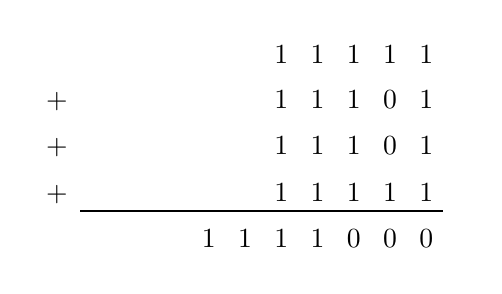
\begin{tikzpicture}[
    every node/.style={column sep=.5mm,row sep=1mm}]
    \matrix (m) [matrix of math nodes,
        nodes in empty cells,
        %nodes=draw
    ] 
    {
        &  &  &  &  &  &  &  & 1 & 1 & 1 & 1 & 1 &     \\
    +   &  &  &  &  &  &  &  & 1 & 1 & 1 & 0 & 1 &            \\
    +   &  &  &  &  &  &  &  & 1 & 1 & 1 & 0 & 1 &            \\
    +   &  &  &  &  &  &  &  & 1 & 1 & 1 & 1 & 1 &            \\
        &  &  &  &  &  & 1 & 1 & 1 & 1 & 0 & 0 &  0&            \\                                                  
    };

    \draw[-,color=black,semithick] (m-4-2.south west) -- (m-4-13.south east);

\end{tikzpicture}
\end{equation*}

The following example demonstrates the entire process by using different colors to distinguish each column and the corresponding carries they produce. Note that the last two digits in the sum are colored black, as they do not result from any specific column but are instead generated solely from the carries.

\begin{equation*}
\begin{tikzpicture}[
    row 1/.style={font=\textsl,font=\tiny, anchor=mid,
        inner sep=1.5pt},
    row 2/.style={font=\textsl,font=\tiny, anchor=mid,
        inner sep=1.5pt},
    row 3/.style={font=\textsl,font=\tiny, anchor=mid,
        inner sep=1.5pt},
    every node/.style={column sep=.5mm,row sep=1mm}]
    \matrix (m) [matrix of math nodes,
        nodes in empty cells,
        %nodes=draw
    ] 
    {
        &   &   &   &   &   &  \textcolor{YellowOrange}{1} &  \textcolor{YellowOrange}{0} &  &  &  &  &   &            \\
        &   &   &   &   &   &  & \textcolor{Purple}{1} & \textcolor{Purple}{0} &  & \textcolor{red}{1}  &  &   &            \\
        &   &   &   &   &   &  &  & \textcolor{Green}{1}  & \textcolor{Green}{1}  & \textcolor{blue}{1}  & \textcolor{blue}{0}  &   &            \\
        &  &  &  &  &  &  &  & \textcolor{YellowOrange}{1} & \textcolor{Purple}{1} & \textcolor{Green}{1}  & \textcolor{red}{1}  & \textcolor{blue}{1} &     \\
    +   &  &  &  &  &  &  &  &  \textcolor{YellowOrange}{1} & \textcolor{Purple}{1} & \textcolor{Green}{1}  & \textcolor{red}{0} & \textcolor{blue}{1}  &            \\
    +   &  &  &  &  &  &  &  &  \textcolor{YellowOrange}{1} & \textcolor{Purple}{1} & \textcolor{Green}{1}  & \textcolor{red}{0}  & \textcolor{blue}{1}  &            \\
    +   &  &  &  &  &  &  &  &  \textcolor{YellowOrange}{1} & \textcolor{Purple}{1} & \textcolor{Green}{1}  & \textcolor{red}{1}  & \textcolor{blue}{1}  &            \\
        &  &  &  &  &  & 1 & 1 &  \textcolor{YellowOrange}{1} & \textcolor{Purple}{1} & \textcolor{Green}{0}  & \textcolor{red}{0}  & \textcolor{blue}{1}  &            \\                                                  
    };

    \draw[-,color=black,semithick] (m-7-2.south west) -- (m-7-13.south east);

\end{tikzpicture}
\end{equation*}

\subsubsection*{Method 2: Direct Summation and Simplification}
We will illustrate the second method using the same example. In the previous case, we carried the actual binary number to the next columns. In this method, we write down 0 if the sum is even and 1 if the sum is odd. Every time a sum a multiple of 2, we carry a 1 to the next columns, and then continue this process for each column, including the carries in the calculation of that column.

\textbf{Step 1: Add the Rightmost Column}\newline
Add bits in column 1 (from counting from MSB):

$$
1+1+1+1=100_2 \quad(\text { which is binary for } 4)
$$
Reading the result from LSB to MSB
\begin{itemize}
    \item write down the 0
    \item carry a 1 for the first multiple of 2
    \item carry a 1 for the second multiple of 2
\end{itemize}
This results in


\begin{equation*}
\begin{tikzpicture}[
    row 1/.style={font=\textsl,font=\tiny, anchor=mid,
        inner sep=1.5pt},
    row 2/.style={font=\textsl,font=\tiny, anchor=mid,
        inner sep=1.5pt},
    row 3/.style={font=\textsl,font=\tiny, anchor=mid,
        inner sep=1.5pt},
    every node/.style={column sep=.5mm,row sep=1mm}]
    \matrix (m) [matrix of math nodes,
        nodes in empty cells,
        %nodes=draw
    ] 
    {
        &   &   &   &   &   &  &  &  &  &  &  &   &            \\
        &   &   &   &   &   &  &  &  &  &  & 1 &   &            \\
        &   &   &   &   &   &  &  & &  &  & 1 &   &            \\
        &  &  &  &  &  &  &  & 1 & 1 & 1 & 1 & 1 &     \\
    +   &  &  &  &  &  &  &  & 1 & 1 & 1 & 0 & 1 &            \\
    +   &  &  &  &  &  &  &  & 1 & 1 & 1 & 0 & 1 &            \\
    +   &  &  &  &  &  &  &  & 1 & 1 & 1 & 1 & 1 &            \\
        &  &  &  &  &  &  &  &  &  &  &  & 0 &            \\                                                  
    };

    \draw[-,color=black,semithick] (m-7-2.south west) -- (m-7-13.south east);

\end{tikzpicture}
\end{equation*}

\textbf{Step 2: Add the Second Column from the Right}\newline
Add bits in column 2 (from counting from MSB):

$$
1+1+1+1=100_2 \quad(\text { which is binary for } 4)
$$
Reading the result from LSB to MSB
\begin{itemize}
    \item write down the 0
    \item carry a 1 for the first multiple of 2
    \item carry a 1 for the second multiple of 2
\end{itemize}
This results in


\begin{equation*}
\begin{tikzpicture}[
    row 1/.style={font=\textsl,font=\tiny, anchor=mid,
        inner sep=1.5pt},
    row 2/.style={font=\textsl,font=\tiny, anchor=mid,
        inner sep=1.5pt},
    row 3/.style={font=\textsl,font=\tiny, anchor=mid,
        inner sep=1.5pt},
    every node/.style={column sep=.5mm,row sep=1mm}]
    \matrix (m) [matrix of math nodes,
        nodes in empty cells,
        %nodes=draw
    ] 
    {
        &   &   &   &   &   &  &  &  &  &  &  &   &            \\
        &   &   &   &   &   &  &  &  &  & 1  &  &   &            \\
        &   &   &   &   &   &  &  & &  & 1 &  &   &            \\
        &  &  &  &  &  &  &  & 1 & 1 & 1 & 1 & 1 &     \\
    +   &  &  &  &  &  &  &  & 1 & 1 & 1 & 0 & 1 &            \\
    +   &  &  &  &  &  &  &  & 1 & 1 & 1 & 0 & 1 &            \\
    +   &  &  &  &  &  &  &  & 1 & 1 & 1 & 1 & 1 &            \\
        &  &  &  &  &  &  &  &  &  &  & 0 & 0 &            \\                                                  
    };

    \draw[-,color=black,semithick] (m-7-2.south west) -- (m-7-13.south east);

\end{tikzpicture}
\end{equation*}

\textbf{Step 3: Add the Third Column from the Right}
Add bits in column 3 (from counting from MSB):

$$
1+1+1+1+1+1=110_2 \quad(\text { which is binary for } 6)
$$
Reading the result from LSB to MSB
\begin{itemize}
    \item write down the 0
    \item carry a 1 for the first multiple of 2
    \item carry a 1 for the second multiple of 2
    \item carry a 1 for the third multiple of 2
\end{itemize}

This results in


\begin{equation*}
\begin{tikzpicture}[
    row 1/.style={font=\textsl,font=\tiny, anchor=mid,
        inner sep=1.5pt},
    row 2/.style={font=\textsl,font=\tiny, anchor=mid,
        inner sep=1.5pt},
    row 3/.style={font=\textsl,font=\tiny, anchor=mid,
        inner sep=1.5pt},
    every node/.style={column sep=.5mm,row sep=1mm}]
    \matrix (m) [matrix of math nodes,
        nodes in empty cells,
        %nodes=draw
    ] 
    {
        &   &   &   &   &   &  &  &  & 1 &  &  &   &            \\
        &   &   &   &   &   &  &  &  & 1 &   &  &   &            \\
        &   &   &   &   &   &  &  & & 1 &  &  &   &            \\
        &  &  &  &  &  &  &  & 1 & 1 & 1 & 1 & 1 &     \\
    +   &  &  &  &  &  &  &  & 1 & 1 & 1 & 0 & 1 &            \\
    +   &  &  &  &  &  &  &  & 1 & 1 & 1 & 0 & 1 &            \\
    +   &  &  &  &  &  &  &  & 1 & 1 & 1 & 1 & 1 &            \\
        &  &  &  &  &  &  &  &  &  & 0 & 0 & 0 &            \\                                                  
    };

    \draw[-,color=black,semithick] (m-7-2.south west) -- (m-7-13.south east);

\end{tikzpicture}
\end{equation*}

\textbf{Step 4: Add the Fourth Column from the Right}\newline
Add bits in column 4 (from counting from MSB):

$$
1+1+1+1+1+1+1=111_2 \quad(\text { which is binary for } 7)
$$
Reading the result from LSB to MSB
\begin{itemize}
    \item write down the 1
    \item carry a 1 for the first multiple of 2
    \item carry a 1 for the second multiple of 2
    \item carry a 1 for the third multiple of 2
\end{itemize}
This results in


\begin{equation*}
\begin{tikzpicture}[
    row 1/.style={font=\textsl,font=\tiny, anchor=mid,
        inner sep=1.5pt},
    row 2/.style={font=\textsl,font=\tiny, anchor=mid,
        inner sep=1.5pt},
    row 3/.style={font=\textsl,font=\tiny, anchor=mid,
        inner sep=1.5pt},
    every node/.style={column sep=.5mm,row sep=1mm}]
    \matrix (m) [matrix of math nodes,
        nodes in empty cells,
        %nodes=draw
    ] 
    {
        &   &   &   &   &   &  &  & 1 &  &  &  &   &            \\
        &   &   &   &   &   &  &  & 1 &  &   &  &   &            \\
        &   &   &   &   &   &  &  & 1 &  &  &  &   &            \\
        &  &  &  &  &  &  &  & 1 & 1 & 1 & 1 & 1 &     \\
    +   &  &  &  &  &  &  &  & 1 & 1 & 1 & 0 & 1 &            \\
    +   &  &  &  &  &  &  &  & 1 & 1 & 1 & 0 & 1 &            \\
    +   &  &  &  &  &  &  &  & 1 & 1 & 1 & 1 & 1 &            \\
        &  &  &  &  &  &  &  &  & 1 & 0 & 0 & 0 &            \\                                                  
    };

    \draw[-,color=black,semithick] (m-7-2.south west) -- (m-7-13.south east);

\end{tikzpicture}
\end{equation*}


\textbf{Step 5: Add the Leftmost Column}\newline
Add bits in leftmost column):

$$
1+1+1+1+1+1+1=111_2 \quad(\text { which is binary for } 7)
$$
Reading the result from LSB to MSB
\begin{itemize}
    \item write down the result in binary, i.e. 1 1 1
\end{itemize}
This results in


\begin{equation*}
\begin{tikzpicture}[
    row 1/.style={font=\textsl,font=\tiny, anchor=mid,
        inner sep=1.5pt},
    row 2/.style={font=\textsl,font=\tiny, anchor=mid,
        inner sep=1.5pt},
    row 3/.style={font=\textsl,font=\tiny, anchor=mid,
        inner sep=1.5pt},
    every node/.style={column sep=.5mm,row sep=1mm}]
    \matrix (m) [matrix of math nodes,
        nodes in empty cells,
        %nodes=draw
    ] 
    {
        &   &   &   &   &   &  &  &  &  &  &  &   &            \\
        &   &   &   &   &   &  &  &  &  &   &  &   &            \\
        &   &   &   &   &   &  &  & &  &  &  &   &            \\
        &  &  &  &  &  &  &  & 1 & 1 & 1 & 1 & 1 &     \\
    +   &  &  &  &  &  &  &  & 1 & 1 & 1 & 0 & 1 &            \\
    +   &  &  &  &  &  &  &  & 1 & 1 & 1 & 0 & 1 &            \\
    +   &  &  &  &  &  &  &  & 1 & 1 & 1 & 1 & 1 &            \\
        &  &  &  &  &  & 1 & 1 & 1 & 1 & 0 & 0 & 0 &            \\                                                  
    };

    \draw[-,color=black,semithick] (m-7-2.south west) -- (m-7-13.south east);
\end{tikzpicture}
\end{equation*}

which corresponds to the result we obtained above. While not demonstrated explicitly here, subtraction works in a similar fashion.

By using one of these methods for handling multiple carries, allow us to also multiply two binary numbers.



\subsection*{Multiplication in Binary}
Multiplication in binary is technically easier than multiplication in decimal. In binary operations, we work exclusively with two digits: 0 and 1. This means that both the the multiplier\footnote{The "multiplicand" is the number that has to be multiplied, and the "multiplier" is the number by which it is multiplied.} and multiplicand consist of 0's and 1' (and so does the multiplicand). The process of finding the binary product is analogous to traditional multiplication in the decimal system. The four five steps involved in multiplying binary digits are:

\[
\begin{aligned}
& 0 \times 0=0 \\
& 0 \times 1=0 \\
& 1 \times 0=0 \\
& 1 \times 1=1 \\
& 1 \times 10_2 = 10_2 \quad \left( \text{multiplying by base } 10_2 \text{ adds a 0 to the end} \right)
\end{aligned}
\]

The last step means that $101_2 \times 10_2 = 1010_2$ which is analogous to the decimal case: $143_{10} \times 10_{10} = 1430_{10}$.

We will illustrate the process by supplying a couple of examples.

\begin{example}


\begin{equation*}
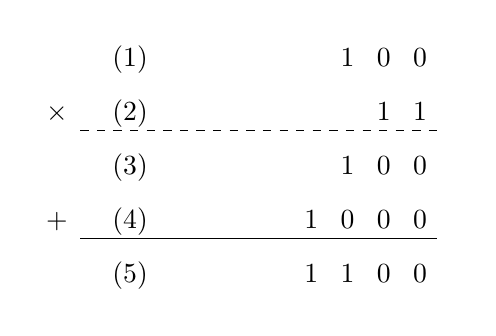
\begin{tikzpicture}[
    every node/.style={column sep=.5mm,row sep=1mm}]
    \matrix (m) [matrix of math nodes,
        nodes in empty cells,
        %nodes=draw
    ] 
    {
        &   &  (1) &   &   &   &  &  &  &  & 1 & 0 & 0  &            \\
     \times   &   & (2)  &   &   &   &  &  &  &  &   & 1 &  1 &            \\
        &   & (3)  &   &   &   &  &  & &  & 1 & 0 & 0  &            \\
       + &  & (4) &  &  &  &  &  &  & 1 & 0 & 0 & 0 &     \\
        &  & (5) &  &  &  &  &  &  & 1 & 1 & 0 & 0 &            \\                                                  
    };

    \draw[dashed, color=black, semithick] (m-2-2.south west) -- (m-2-13.south east);
    \draw[-,color=black,semithick] (m-4-2.south west) -- (m-4-13.south east);
    \end{tikzpicture}
\end{equation*}

Here are the steps:

\begin{itemize}
    \item Multiply the multiplicand (line 1) by the LSB of the multiplier (line 2), which in this case is 1.
    \item Record this result in line 3.
    \item Append a 0 to line 4 to account for the shift to the next power of 2 in the multiplier.
    \item Multiply the multiplicand (line 1) by the next bit of the multiplier (line 2), which is also 1 in this case.
    \item Add this result to line 4, after the 0 you appended earlier.
    \item Finally, sum the values in lines 3 and 4, as outlined in the previous section, to obtain the final result in line 5.
\end{itemize}
\end{example}

We offer two additional examples:

\begin{example}

\begin{equation*}
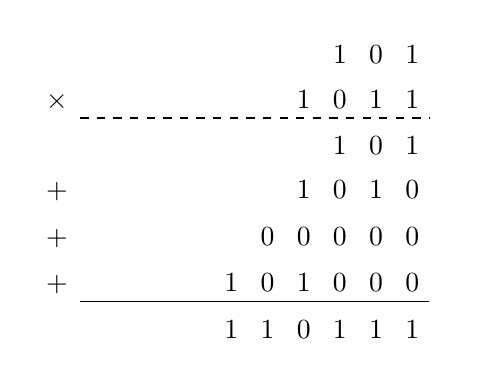
\begin{tikzpicture}[
    every node/.style={column sep=.5mm,row sep=1mm}]
    \matrix (m) [matrix of math nodes,
        nodes in empty cells,
        %nodes=draw
    ] 
    {
        &   &   &   &   &   &  &  &  &  & 1 & 0 & 1  &            \\
     \times   &   &   &   &   &   &  &  &  & 1 &  0 & 1 &  1 &            \\
        &   &   &   &   &   &  &  & &  & 1 & 0 & 1  &            \\
       + &  &  &  &  &  &  &  &  & 1 & 0 & 1 & 0 &     \\
       + &  &  &  &  &  &  &  & 0 & 0 & 0 & 0 & 0 &            \\               
       + &  &  &  &  &  &  & 1 & 0 & 1 & 0 & 0 & 0 &     \\
        &  &  &  &  &  &  & 1 & 1 & 0 & 1 & 1 & 1 &            \\                                        
    };

    \draw[dashed, color=black, semithick] (m-2-2.south west) -- (m-2-13.south east);
    \draw[-,color=black,semithick] (m-6-2.south west) -- (m-6-13.south east);
    \end{tikzpicture}
\end{equation*}
    
\end{example}

\begin{example}
\label{ex1.3}
\begin{equation*}
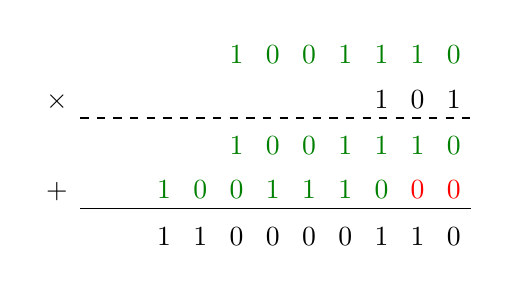
\begin{tikzpicture}[
    every node/.style={column sep=.5mm,row sep=1mm}]
    \matrix (m) [matrix of math nodes,
        nodes in empty cells,
        %nodes=draw
    ] 
    {
        &   &   &   &   &   & \textcolor{Green}{1} & \textcolor{Green}{0} & \textcolor{Green}{0} & \textcolor{Green}{1} & \textcolor{Green}{1} & \textcolor{Green}{1} & \textcolor{Green}{0}  &            \\
     \times   &   &   &   &   &   &  &  &  &  &  1 & 0 &  1 &            \\
        &   &   &   &   &   & \textcolor{Green}{1} & \textcolor{Green}{0} & \textcolor{Green}{0} & \textcolor{Green}{1} & \textcolor{Green}{1} & \textcolor{Green}{1} & \textcolor{Green}{0}   &            \\
       + &  &  &  & \textcolor{Green}{1} & \textcolor{Green}{0} & \textcolor{Green}{0} & \textcolor{Green}{1} & \textcolor{Green}{1} & \textcolor{Green}{1} & \textcolor{Green}{0} & \textcolor{Red}{0} & \textcolor{Red}{0} &            \\             
        &  &  &  & 1 & 1 & 0 & 0 & 0 & 0 & 1 & 1 & 0 &     \\                                     
    };

    \draw[dashed, color=black, semithick] (m-2-2.south west) -- (m-2-13.south east);
    \draw[-,color=black,semithick] (m-4-2.south west) -- (m-4-13.south east);
    \end{tikzpicture}
\end{equation*}
    
\end{example}

In \autoref{ex1.3} notice that we omitted the row of zeroes that the second value of the multiplier would have produced, and notice even further that we added two 0's before restating the multiplicand in the sum.

Binary multiplication, like binary addition, is a core operation in computer arithmetic. By breaking the process down into manageable steps—multiplying individual bits and then summing the results—it becomes clear how similar it is to the multiplication methods we use in the decimal system. The main difference is the simplicity and efficiency of working within the binary system, where only the digits 0 and 1 are involved.

We notice how binary multiplication builds on binary addition. Each step, involving shifts and sums, essentially consists of repeated additions adjusted by powers of two. A strong grasp of binary addition naturally leads to a better understanding of binary multiplication and its applications.

\section{Octal and Hexadecimal}
Octal is a base-8 numbering system that uses the digits 0 through 7. It is closely related to binary, which is a base-2 system. The connection between the two lies in how easily binary numbers can be converted to octal and vice versa. Each octal digit corresponds to exactly three binary digits (bits), making conversions straightforward. For example, the binary number `110` converts directly to the octal digit `6`. Because of this close relationship, octal is often used as a shorthand for binary in computing, particularly in contexts where grouping binary digits in sets of three simplifies reading and interpreting binary data.

\[
\begin{aligned}
12_8 &= 1 \cdot 8^1 + 2 \cdot 8^0  = 10_{10} \\
3021_8 & = 3 \cdot 8^3 + 0 \cdot 8^2 + 2 \cdot 8^1 + 1 \cdot 8^0 = 1553_{10}
\end{aligned}
\]

Since \(8\) is \(2^3\), we can express it in binary:

\[
\begin{aligned}
3 & \rightarrow \textcolor{Green}{011} \\
0 & \rightarrow \textcolor{YellowOrange}{000} \\
2 & \rightarrow \textcolor{blue}{010} \\
1 & \rightarrow \textcolor{red}{001} \\
\end{aligned}
\]

\[
\text{Thus, } 3021_8 = \textcolor{Green}{011}\textcolor{YellowOrange}{000} \textcolor{blue}{010}\textcolor{red}{001}_2 = \textcolor{Green}{11}\textcolor{YellowOrange}{000} \textcolor{blue}{010}\textcolor{red}{001}_2
\]

We obtain the final result by removing leading zeros.

Hexadecimal is a base-16 numbering system that uses sixteen distinct symbols: the digits 0-9 and the letters A-F, where A represents 10, B represents 11, and so on up to F, which represents 15. Hexadecimal is closely related to binary because each hexadecimal digit corresponds exactly to four binary digits (bits). This direct relationship makes it easy to convert between the two systems. For example, the hexadecimal digit `A` translates to the binary sequence `1010`. Due to this efficiency in grouping, hexadecimal is often used in computing as a more compact and readable way to represent binary data, particularly in areas like memory addresses and colour codes in web design.

\[
\begin{aligned}
123_{16} &= 1 \cdot 16^2 + 2 \cdot 16^1 + 3 \cdot 16^0  = 256 + 32 + 3 = 291_{10} \\
A2E_{16} & = 10 \cdot 16^2 + 2 \cdot 16^1 + 14 \cdot 16^0 = 2560 + 32 + 14 = 2606_{10}
\end{aligned}
\]

Since \(16\) is \(2^4\), we can, for instance, express $A2E_{16}$ in binary:

\[
\begin{aligned}
A & \rightarrow 1010 \\
2 & \rightarrow 0010 \\
E & \rightarrow 1110 \\
\end{aligned}
\]

\[
\text{Thus, } A2E_{16} = 101000101110_2
\]

Similarly we get $5EB52_{16}$ as

\[
\begin{aligned}
5 & \rightarrow 0101 \\
E & \rightarrow 1110 \\
B & \rightarrow 1011 \\
5 & \rightarrow 0101 \\
2 & \rightarrow 0010 \\
\end{aligned}
\]

\[
\text{Thus, } 5EB52_{16} = 01011110101101010010_2
\]

Again, notice that we removed the leading 0's from $5_{16}$ when writing the result.

\section{Converting Between Systems}

Understanding how to convert numbers between binary, decimal, octal, and hexadecimal systems is essential in computer science and digital electronics. Each system is a different base, and each has its own applications. Here's a step-by-step guide to help you convert numbers from one system to another.

\subsection*{Decimal to Binary Conversion}
To convert a decimal number to binary:
\begin{enumerate}
    \item Divide the decimal number by 2.
    \item Record the remainder (it will be 0 or 1).
    \item Divide the quotient by 2 and record the remainder.
    \item Repeat until the quotient is 0.
    \item The binary number is the sequence of remainders read from bottom to top.
\end{enumerate}

\begin{example} Convert \(23_{10}\) to binary.

\begin{solution}

\[
\begin{aligned}
23 \div 2 & = 11 \quad \text{remainder } 1 \\
11 \div 2 & = 5 \quad \text{remainder } 1 \\
5 \div 2 & = 2 \quad \text{remainder } 1 \\
2 \div 2 & = 1 \quad \text{remainder } 0 \\
1 \div 2 & = 0 \quad \text{remainder } 1 \\
\end{aligned}
\]
Thus, \(23_{10} = 10111_2\). \end{solution}
\end{example}

\subsection*{Decimal to Octal Conversion}
To convert a decimal number to octal:
\begin{enumerate}
    \item Divide the decimal number by 8.
    \item Record the remainder.
    \item Divide the quotient by 8 and record the remainder.
    \item Repeat until the quotient is 0.
    \item The octal number is the sequence of remainders read from bottom to top.
\end{enumerate}

\begin{example}Convert \(78_{10}\) to octal.

\begin{solution}
    


\[
\begin{aligned}
78 \div 8 & = 9 \quad \text{remainder } 6 \\
9 \div 8 & = 1 \quad \text{remainder } 1 \\
1 \div 8 & = 0 \quad \text{remainder } 1 \\
\end{aligned}
\]
Thus, \(78_{10} = 116_8\). \end{solution}
    
\end{example}

\subsection*{Decimal to Hexadecimal Conversion}
To convert a decimal number to hexadecimal:
\begin{enumerate}
    \item Divide the decimal number by 16.
    \item Record the remainder (use A, B, C, D, E, F for remainders 10, 11, 12, 13, 14, 15 respectively).
    \item Divide the quotient by 16 and record the remainder.
    \item Repeat until the quotient is 0.
    \item The hexadecimal number is the sequence of remainders read from bottom to top.
\end{enumerate}

\begin{example}Convert \(255_{10}\) to hexadecimal.

\begin{solution}
    
\[
\begin{aligned}
255 \div 16 & = 15 \quad \text{remainder } 15 \quad (\text{F}) \\
15 \div 16 & = 0 \quad \text{remainder } 15 \quad (\text{F}) \\
\end{aligned}
\]
Thus, \(255_{10} = FF_{16}\).\end{solution}

\end{example}


\subsection*{Binary to Decimal Conversion}
To convert a binary number to decimal:
\begin{enumerate}
    \item Multiply each bit by 2 raised to the power of its position, starting from 0 on the right.
    \item Sum all the products.
\end{enumerate}

Notice that this amounts to the method outlined above about binary expansion.

\begin{example} Convert \(1101_2\) to decimal.

\begin{solution}
    

\[
\begin{aligned}
1 \cdot 2^3 + 1 \cdot 2^2 + 0 \cdot 2^1 + 1 \cdot 2^0 & = 8 + 4 + 0 + 1 = 13_{10}
\end{aligned}
\] \end{solution}

\end{example}

\subsection*{Binary to Octal Conversion}
To convert a binary number to octal:
\begin{enumerate}
    \item Group the binary digits into sets of three, starting from the right. Add leading zeros if necessary.
    \item Convert each group of three binary digits to its octal equivalent.
\end{enumerate}

\begin{example}Convert \(110110_2\) to octal.

\begin{solution}
\[
\begin{aligned}
110 & \rightarrow 6 \\
110 & \rightarrow 6 \\
\end{aligned}
\]
Thus, \(110110_2 = 66_8\). \end{solution}

\end{example}

\subsection*{Binary to Hexadecimal Conversion}
To convert a binary number to hexadecimal:
\begin{enumerate}
    \item Group the binary digits into sets of four, starting from the right. Add leading zeros if necessary.
    \item Convert each group of four binary digits to its hexadecimal equivalent.
\end{enumerate}

\begin{example}Convert \(10110101_2\) to hexadecimal.

\begin{solution}
\[
\begin{aligned}
1011 & \rightarrow B \\
0101 & \rightarrow 5 \\
\end{aligned}
\]
Thus, \(10110101_2 = B5_{16}\). \end{solution}

\end{example}

\subsection*{Octal to Binary Conversion}
To convert an octal number to binary: Convert each octal digit to its 3-bit binary equivalent!

\begin{example}Convert \(57_8\) to binary.

\begin{solution}
\[
\begin{aligned}
5 & \rightarrow 101 \\
7 & \rightarrow 111 \\
\end{aligned}
\]
Thus, \(57_8 = 101111_2\). \end{solution}

\end{example}

\subsection*{Octal to Decimal Conversion}
To convert an octal number to decimal:
\begin{enumerate}
    \item Multiply each digit by 8 raised to the power of its position, starting from 0 on the right.
    \item Sum all the products.
\end{enumerate}

\begin{example}Convert \(157_8\) to decimal.

\begin{solution}
    
\[
\begin{aligned}
1 \cdot 8^2 + 5 \cdot 8^1 + 7 \cdot 8^0 & = 64 + 40 + 7 = 111_{10}
\end{aligned}
\] \end{solution}

\end{example}

\subsection*{Octal to Hexadecimal Conversion}
To convert an octal number to hexadecimal:
\begin{enumerate}
    \item First, convert the octal number to binary.
    \item Then, convert the binary number to hexadecimal by grouping the binary digits in sets of four.
\end{enumerate}

\begin{example}Convert \(157_8\) to hexadecimal.

\begin{solution}

\[
\begin{aligned}
1 & \rightarrow 001 \\
5 & \rightarrow 101 \\
7 & \rightarrow 111 \\
\end{aligned}
\]
Thus, \(157_8 = 001101111_2 = 6F_{16}\). \end{solution}
\end{example}

\subsection*{Hexadecimal to Binary Conversion}
To convert a hexadecimal number to binary: Convert each hexadecimal digit to its 4-bit binary equivalent.

\begin{example}Convert \(2B_{16}\) to binary.

\begin{solution}
    


\[
\begin{aligned}
2 & \rightarrow 0010 \\
B & \rightarrow 1011 \\
\end{aligned}
\]
Thus, \(2B_{16} = 00101011_2\).\end{solution}

\end{example}

\subsection*{Hexadecimal to Decimal Conversion}
To convert a hexadecimal number to decimal:
\begin{enumerate}
    \item Multiply each digit by 16 raised to the power of its position, starting from 0 on the right.
    \item Sum all the products.
\end{enumerate}

\begin{example}Convert \(2B_{16}\) to decimal.

\begin{solution}
\[
\begin{aligned}
2 \cdot 16^1 + 11 \cdot 16^0 & = 32 + 11 = 43_{10}
\end{aligned}
\] \end{solution}
\end{example}

\subsection*{Hexadecimal to Octal Conversion}
To convert a hexadecimal number to octal:
\begin{enumerate}
    \item First, convert the hexadecimal number to binary.
    \item Then, convert the binary number to octal by grouping the binary digits in sets of three.
\end{enumerate}

\begin{example}Convert \(2B_16\) to octal.

\begin{solution}

\[
\begin{aligned}
2 & \rightarrow 0010 \\
B & \rightarrow 1011 \\
\end{aligned}
\]
Thus, \(2B_{16} = 00101011_2 = 53_8\). \end{solution}

\end{example}

\subsection*{Final Thoughts on Conversion}
The concept of expansion plays a central role in these conversions. Whether you are expanding a decimal number into its binary, octal, or hexadecimal form, or converting a binary number into its octal or hexadecimal equivalent, you are more or less expressing the number in terms of powers of the base. The expansion method is essentially the same for each system as it boils down to dividing by the highest power of the base recursively:

$$
\begin{aligned}
7562_{10} & =1 \cdot 16^3+3466=1 \cdot 16^3+13 \cdot 16^2+138 \\
& =\textcolor{red}{1} \cdot 16^3+ \textcolor{blue}{13} \cdot 16^2+\textcolor{YellowOrange}{8} \cdot 16^1+\textcolor{Green}{10} \cdot 16^0=\textcolor{red}{1} \, \textcolor{blue}{D} \, \textcolor{YellowOrange}{8} \, \textcolor{Green}{A}
\end{aligned}
$$

By understanding these expansions and the relationships between these number systems, you can efficiently switch between them, allowing you to represent and manipulate data in the most suitable format for any given situation.

\chapter{Set Theory}
\label{chap:ch3}

In software engineering, we are constantly working with collections of things: users in a system, records in a database, or nodes in a network. Set theory provides the formal mathematical language to describe and manipulate these collections with precision and clarity. It is the bedrock upon which many core computer science concepts—from database query languages like SQL to data structures and algorithmic logic—are built.

This chapter introduces the fundamental principles of set theory. We will begin with the simple, intuitive idea of a set and explore the formal notation used to define them. We will then cover the essential relationships between sets, such as subsets, and the core operations used to combine them, including unions, intersections, and complements. These operations directly correspond to the logical operators (\texttt{OR}, \texttt{AND}, \texttt{NOT}) that govern the flow of your code. Finally, we will explore ordered collections called tuples and introduce a simple method for proving set equalities.

\section{What is a Set?}
A set is an unordered collection of distinct objects. The objects within a set are called its \textbf{elements} or \textbf{members}. We can think of a set as a simple container where items are grouped together, and the order in which we list them does not matter. For example, the set of primary colors can be written as $\{ \text{red}, \text{yellow}, \text{blue} \}$ or equally as $\{ \text{blue}, \text{red}, \text{yellow} \}$.

Sets are a cornerstone of modern mathematics and a fundamental concept in computer science. They form the logical basis for everything from database query languages and data structures to the specification of programming language types.

% --- Figure Placeholder ---
% This figure illustrates the basic concept of a set.
% It is inspired by Slide 3 of your PowerPoint presentation.
\begin{figure}[htbp]
    \centering
    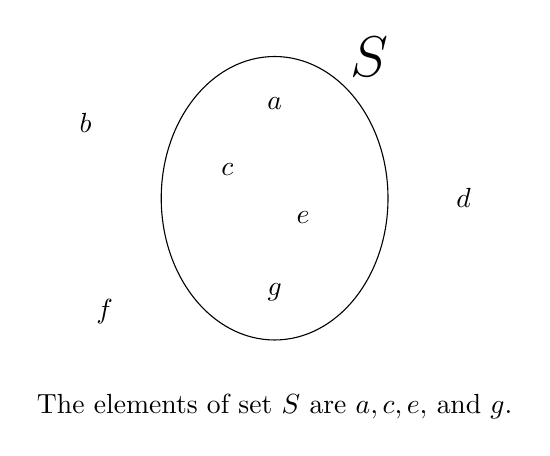
\begin{tikzpicture}[scale=1.2]
        % The set S as an ellipse
        \draw (0,0) ellipse (1.2cm and 1.5cm);
        \node at (1, 1.5) {\huge $S$};
        
        % Elements inside the set S
        \node at (0, 1) {$a$};
        \node at (-0.5, 0.3) {$c$};
        \node at (0.3, -0.2) {$e$};
        \node at (0, -1) {$g$};
        
        % Elements outside the set S
        \node at (-2, 0.8) {$b$};
        \node at (-1.8, -1.2) {$f$};
        \node at (2, 0) {$d$};

        % Annotation
        \node[align=center] at (0,-2.2) {The elements of set $S$ are $a, c, e,$ and $g$.};
    \end{tikzpicture}
    \caption{A set $S$ containing four elements. The objects $b, d,$ and $f$ are not elements of $S$.}
    \label{fig:set_concept}
\end{figure}

\subsection*{Specifying a Set}
There are two primary ways to describe a set: by explicitly listing its members or by defining a property that its members must satisfy.

\subsubsection*{Listing Notation (Roster Method)}
The most direct way to define a set is by listing all its elements between curly braces, $\{ \}$. This is known as the \textbf{roster method}.

For example:
\begin{itemize}
    \item The set of the first five letters of the alphabet is $A = \{a, b, c, d, e\}$.
    \item The set of the first three positive integers is $C = \{1, 2, 3\}$.
    \item A set can contain different types of elements: $D = \{ \text{Alice}, 42, \pi \}$.
\end{itemize}

When using the roster method, there are two fundamental rules:
\begin{enumerate}
    \item \textbf{Order does not matter.} A set is defined only by the elements it contains, not by the sequence in which they are listed. For example, $\{1, 2, 3\}$ is the exact same set as $\{3, 1, 2\}$.
    \item \textbf{Each element must be unique.} An element is either in a set or it is not. Listing an element more than once is redundant and does not change the set. For instance, the set $\{a, a, b, c, c\}$ is simply $\{a, b, c\}$.
\end{enumerate}


\subsubsection*{Set-Builder Notation}
When listing every element is impractical or impossible (for example, with infinite sets), we use \textbf{set-builder notation}. This method defines a set by stating a property or rule that its elements must satisfy. The notation uses a vertical bar `|` or a colon `:`, which is read as "such that."

The general structure is:
\[ \{ \text{variable} \mid \text{a property the variable must satisfy} \} \]

For example:
\begin{itemize}
    \item $A = \{ l \mid l \text{ is a vowel in the English alphabet} \}$ \\
    This is read as: "$A$ is the set of all elements $l$ such that $l$ is a vowel in the English alphabet." This is another way of writing $A = \{a, e, i, o, u\}$.
    
    \item $C = \{ n \mid n \in \mathbb{Z} \text{ and } 0 < n < 4 \}$ \\
    This is read as: "$C$ is the set of all numbers $n$ such that $n$ is an integer and $n$ is greater than 0 and less than 4." This defines the set $\{1, 2, 3\}$.
    
    \item $E = \{ x \mid x \text{ is an even integer} \}$ \\
    This defines the infinite set of all even integers: $\{\dots, -4, -2, 0, 2, 4, \dots\}$.
\end{itemize}

Set-builder notation is extremely powerful because it allows us to define large, complex, or even infinite sets with a short and precise description.

\section{Important Sets: The Number Systems}
Numbers are the foundation of mathematics and computation. The different categories of numbers we use every day, from counting items to measuring continuous values, can be formally defined as sets. Understanding these fundamental sets is crucial for any software engineer, as they underpin data types, arithmetic logic, and numerical algorithms.

\subsection*{The Main Number Sets}
The following sets are some of the most important in mathematics and are used throughout science and engineering.

\begin{description}
    \item[Natural Numbers ($\mathbb{N}$)] The set of positive integers used for counting: $\{1, 2, 3, \dots\}$. Sometimes, this set is defined to include $0$. Due to this ambiguity, it is often clearer to specify \textit{positive integers} or \textit{non-negative integers}.

    \item[Integers ($\mathbb{Z}$)] The set of all positive and negative whole numbers, including zero: $\{\dots, -2, -1, 0, 1, 2, \dots\}$.

    \item[Rational Numbers ($\mathbb{Q}$)] The set of all numbers that can be expressed as a fraction $\frac{p}{q}$, where $p$ and $q$ are integers and $q \neq 0$. This includes all integers and terminating or repeating decimals. Examples: $\frac{1}{2}$, $-5$, $0.25$.

    \item[Real Numbers ($\mathbb{R}$)] The set of all numbers on the number line. It includes both rational numbers and irrational numbers (like $\pi$ or $\sqrt{2}$), which cannot be expressed as simple fractions.
    
    \item[Complex Numbers ($\mathbb{C}$)] The set of all numbers that can be expressed in the form $a + bi$, where $a$ and $b$ are real numbers and $i$ is the imaginary unit, satisfying $i^2 = -1$.
\end{description}

Visualizing the relationships between these sets is key to understanding them. A Venn diagram shows the hierarchy of how these sets are nested within one another, while a number line illustrates how they cover or populate the continuum of values.

% --- Venn Diagram of Number Systems ---
% This is the TikZ code you provided for the number system Venn diagram.
\begin{figure}[htbp]
    \centering
    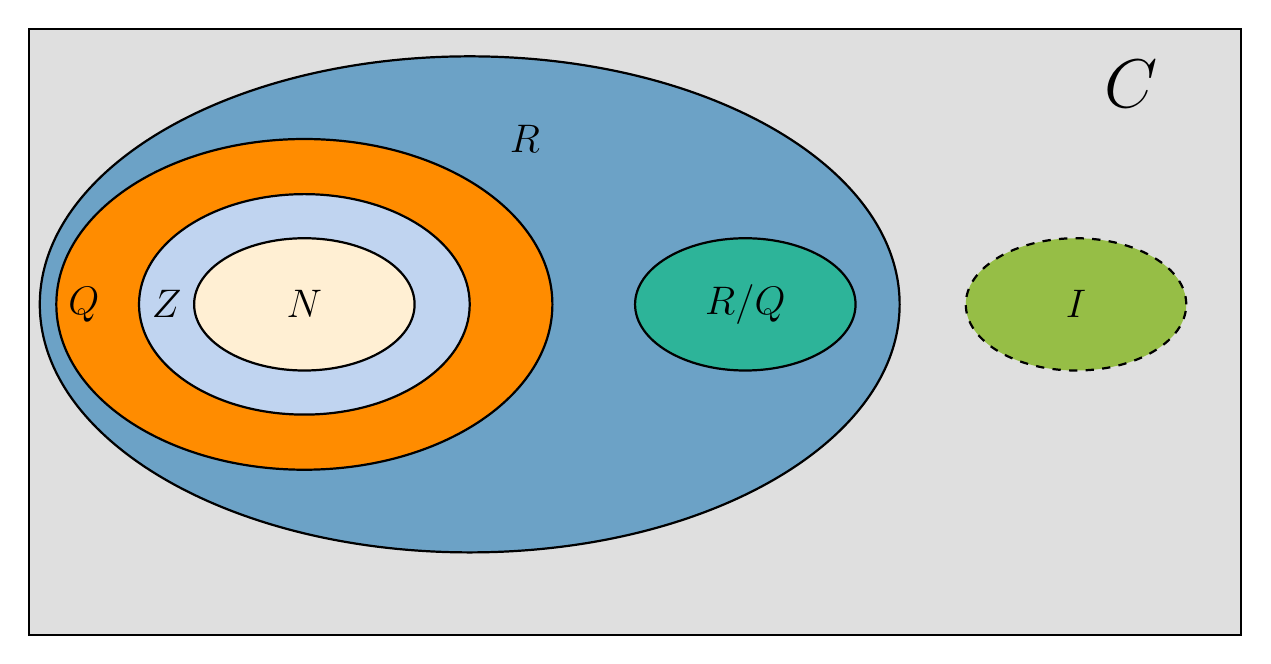
\begin{tikzpicture}[scale=0.7]
        % Complex Numbers (outer square)
        \draw[thick, fill=lightgray!50] (-12, -6) rectangle (10, 5);
        \node at (8, 4) {\Huge $\mathbb{C}$};
        
        % Real Numbers (largest set)
        \draw[thick, fill=mseViaBlue] (-4,0) ellipse (7.8cm and 4.5cm);
        \node at (-3, 3) {\Large $\mathbb{R}$};
        
        % Rational Numbers
        \draw[thick, fill=mseOrange] (-7,0) ellipse (4.5cm and 3cm);
        \node at (-11, 0) {\Large$\mathbb{Q}$};
        
        % Integers
        \draw[thick, fill=mseDarkText] (-7,0) ellipse (3cm and 2cm);
        \node at (-9.5, 0) {\Large$\mathbb{Z}$};
        
        % Natural Numbers
        \draw[thick, fill=mseAnswerBg] (-7,0) ellipse (2cm and 1.2cm);
        \node at (-7, 0) {\Large$\mathbb{N}$};
        
        % Irrational Numbers
        \draw[thick, fill=mseQuestionBorder] (1,0) ellipse (2cm and 1.2cm);
        \node at (1, 0) {\Large$\mathbb{R} /\mathbb{Q} $};
        
        % Imaginary Numbers
        \draw[thick, dashed, fill=mseImaginary] (7,0) ellipse (2cm and 1.2cm);
        \node at (7, 0) {\Large $\mathbb{I}$};
    \end{tikzpicture}
    \caption{A Venn diagram illustrating the hierarchical relationship between the major number sets.}
    \label{fig:venn_num}
\end{figure}

\begin{remark}
    The Venn diagram in \autoref{fig:venn_num} shows that the set of real numbers ($\mathbb{R}$) is composed exclusively of rational ($\mathbb{Q}$) and irrational numbers. There is no real number that is not one or the other. This is why the set of irrational numbers is formally denoted as $\mathbb{R} \setminus \mathbb{Q}$, which means "the set of all real numbers, excluding the rational numbers."
\end{remark}

% --- The Number Line ---
% This figure is inspired by Slide 9 of your PowerPoint presentation.
\begin{figure}[htbp]
    \centering
    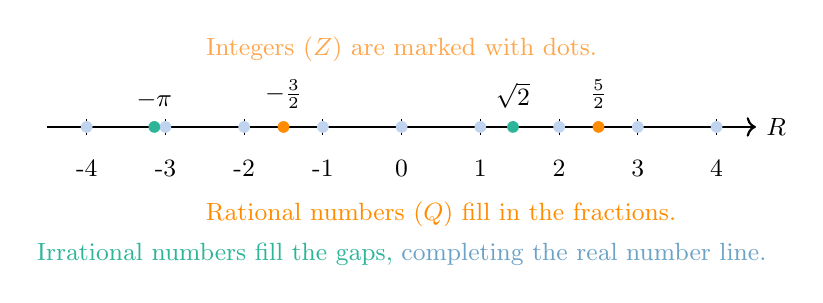
\begin{tikzpicture}[
        every node/.style={font=\small},
        axis/.style={->, thick},
        tick/.style={black, thick},
        dot/.style={circle, fill, inner sep=1.5pt},
        integer/.style={circle, fill=mseDarkText, inner sep=1.5pt},
        rational/.style={circle, fill=mseOrange, inner sep=1.5pt},
        irrational/.style={circle, fill=mseQuestionBorder, inner sep=1.5pt}
    ]
        % Axis line
        \draw[axis] (-4.5,0) -- (4.5,0) node[right]{$\mathbb{R}$};
        
        % Ticks and labels for integers
        \foreach \x in {-4,...,4}{
            \draw (\x, 0.1) -- (\x, -0.1);
            \node[below] at (\x, -0.3) {\x};
            \node[integer] at (\x, 0) {};
        }

        % Annotations for different number sets (properly spaced)
        \node[above=20pt, color=orange!70] at (0,0) {Integers ($\mathbb{Z}$) are marked with dots.};
        
        % Example rational numbers
        \node[rational] at (2.5, 0){};
        \node[above=3pt] at (2.5, 0){$\frac{5}{2}$};
        \node[rational] at (-1.5, 0){};
        \node[above=3pt] at (-1.5, 0){$-\frac{3}{2}$};
        \node[below=15pt, color=mseOrange] at (0.5,-0.3) {Rational numbers ($\mathbb{Q}$) fill in the fractions.};
        
        % Example irrational numbers
        \node[irrational] at (1.414, 0){};
        \node[above=3pt] at (1.414, 0){$\sqrt{2}$};
        \node[irrational] at (-3.141, 0){};
        \node[above=3pt] at (-3.141, 0){$-\pi$};
        \node[below=30pt] at (0,-0.3) {\textcolor{mseQuestionBorder}{Irrational numbers fill the gaps,} \textcolor{mseViaBlue}{completing the real number line.}};
        
    \end{tikzpicture}
    \caption{The real number line, populated by integers, rationals, and irrationals.}
    \label{fig:number_line}
\end{figure}


\subsection*{Interval Notation}
In many applications, we need to refer to a continuous range of real numbers. \textbf{Interval notation} is a convenient shorthand for describing such subsets of $\mathbb{R}$.

An interval is defined by its two endpoints. We use square brackets `[` `]` to indicate that an endpoint is included in the set, and parentheses `(` `)` to indicate that it is excluded.

\begin{description}
    \item[Closed Interval:] Includes both endpoints.
    \[ [a, b] = \{ x \in \mathbb{R} \mid a \leq x \leq b \} \]

    \item[Open Interval:] Excludes both endpoints.
    \[ (a, b) = \{ x \in \mathbb{R} \mid a < x < b \} \]

    \item[Half-Open Intervals:] Includes one endpoint but not the other.
    \[ [a, b) = \{ x \in \mathbb{R} \mid a \leq x < b \} \quad \text{and} \quad (a, b] = \{ x \in \mathbb{R} \mid a < x \leq b \} \]
\end{description}

\begin{example} Interval Notation
\begin{itemize}
    \item $[-2, 3]$ is the set of all real numbers from $-2$ to $3$, including $-2$ and $3$.
    \item $(-2, 3)$ is the set of all real numbers between $-2$ and $3$.
    \item $[0, 100)$ represents all numbers from $0$ up to (but not including) $100$.
\end{itemize}
\end{example}

Intervals can also be unbounded, extending towards positive or negative infinity ($\infty$). Since infinity is not a number, it is always excluded with a parenthesis.
\[ (a, \infty) = \{ x \in \mathbb{R} \mid x > a \} \quad \text{and} \quad (-\infty, b] = \{ x \in \mathbb{R} \mid x \leq b \} \]

\begin{example} Unbounded Interval
\begin{itemize}
    \item $(3, \infty)$ represents all real numbers greater than $3$.
    \item $(-\infty, 5)$ represents all real numbers less than $5$.
    \item $(-\infty, 0]$ represents the set of all non-positive real numbers.
\end{itemize}
\end{example}

%======================================================================
% SECTION: Relationships Between Sets
%======================================================================
\section{Relationships Between Sets}
Understanding a set is not just about its elements, but also how it relates to other sets. This section defines the fundamental relationships that allow us to compare and classify sets.

\subsection*{Subsets and Proper Subsets}
One of the most basic relationships is that of inclusion, where one set is contained within another.

\begin{definition}[Subset]
    A set $A$ is a \textbf{subset} of a set $B$ if every element of $A$ is also an element of $B$. We write this as $A \subseteq B$.
\end{definition}

For example, if $A = \{1, 2\}$ and $B = \{1, 2, 3\}$, then $A \subseteq B$ because every element in $A$ is also in $B$. By this definition, every set is a subset of itself (i.e., $A \subseteq A$).

% --- Subset Figure ---
\begin{figure}[htbp]
    \centering
    \begin{tikzpicture}
        % Set B (the larger set)
        \draw[thick, mseDarkBlue] (0,0) ellipse (2.5cm and 1.8cm);
        \node[mseDarkBlue, above right] at (2.2, 1.2) {$B$};
        
        % Set A (the subset)
        \draw[thick, color=fourth] (-0.5, 0) ellipse (1.2cm and 0.8cm);
        \node[color=fourth] at (0.3, 0.3) {$A$};
        
        % Elements
        \node at (-0.8, 0.1) {$a$};
        \node at (0, -0.1) {$b$};
        \node at (1.5, 0.5) {$c$};
        \node at (-1.5, -1) {$d$};
    \end{tikzpicture}
    \caption{Set $A = \{a, b\}$ is a subset of set $B = \{a, b, c, d\}$, denoted $A \subseteq B$.}
    \label{fig:subset}
\end{figure}

Sometimes we want to specify that a set is a subset of another but is not equal to it.

\begin{definition}[Proper Subset]
    A set $A$ is a \textbf{proper subset} of a set $B$ if $A \subseteq B$ and $A \neq B$. This means that $B$ must contain at least one element that is not in $A$. We write this as $A \subset B$.
\end{definition}

Using the previous example, since $B$ contains the element $3$ which is not in $A$, we can say that $A$ is a proper subset of $B$, or $A \subset B$.

\subsection*{The Universal Set and the Empty Set}
Two special sets act as the boundaries for set theory: the set containing everything and the set containing nothing.

\begin{definition}[Universal Set]
    The \textbf{universal set}, denoted by $U$, is the set of all possible elements under consideration in a given context. All other sets in that context are considered subsets of the universal set.
\end{definition}

The universal set is represented in Venn diagrams by a rectangle that encloses all other sets. For example, if we are discussing integers, the universal set would be $U = \mathbb{Z}$. If we were discussing students at a university, $U$ would be the set of all enrolled students.

% --- Universal and Empty Set Figure ---
\begin{figure}[htbp]
    \centering
    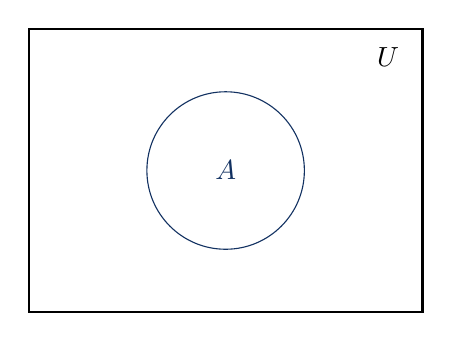
\begin{tikzpicture}
        % Universal Set U
        \draw[thick] (-2.5, -1.8) rectangle (2.5, 1.8);
        \node[above right] at (1.8, 1.2) {$U$};
        
        % A regular set A
        \draw[mseDarkBlue] (0,0) circle (1cm);
        \node[mseDarkBlue] at (0,0) {$A$};
    \end{tikzpicture}
    \caption{The universal set $U$ contains all elements and sets under consideration.}
    \label{fig:universal_set}
\end{figure}

\begin{definition}[Empty Set]
    The \textbf{empty set} (or \textbf{null set}) is the unique set containing no elements. It is denoted by $\emptyset$ or by $\{\}$.
\end{definition}

The empty set has a crucial property:
\begin{center}
    \textit{The empty set is a subset of every set.}
\end{center}
This is because there are no elements in $\emptyset$ that are not in any other set $A$. Therefore, for any set $A$, it is always true that $\emptyset \subseteq A$.

\subsection*{Disjoint Sets}
Sometimes, sets have no relationship at all because they are entirely separate.

\begin{definition}[Disjoint Sets]
    Two sets, $A$ and $B$, are \textbf{disjoint} if they have no elements in common. In other words, their intersection is the empty set: $A \cap B = \emptyset$.
\end{definition}

For example, the set of even integers $E = \{\dots, -2, 0, 2, \dots\}$ and the set of odd integers $O = \{\dots, -3, -1, 1, 3, \dots\}$ are disjoint.

% --- Disjoint Sets Figure ---
\begin{figure}[htbp]
    \centering
    \begin{tikzpicture}
        % Set A
        \draw[thick, mseDarkBlue] (-1.2, 0) circle (1cm);
        \node[mseDarkBlue] at (-1.2, 0) {$A$};
        
        % Set B
        \draw[thick, color=fourth] (1.2, 0) circle (1cm);
        \node[color=fourth] at (1.2, 0) {$B$};
        
        % Caption Label
        \node at (0, -1.5) {Disjoint Sets};
    \end{tikzpicture}
    \caption{Sets $A$ and $B$ are disjoint because they do not overlap.}
    \label{fig:disjoint_sets}
\end{figure}

%======================================================================
% SECTION: Properties of Sets
%======================================================================
\section{Properties of Sets}
Beyond the relationships between sets, we can also describe their intrinsic properties. The two most fundamental properties are a set's size (its cardinality) and the collection of all its possible subsets (its power set).

\subsection*{Cardinality}
The most basic property of a finite set is its size.

\begin{definition}[Cardinality]
    The \textbf{cardinality} of a finite set $A$, denoted $|A|$, is the number of distinct elements in the set.
\end{definition}

For example:
\begin{itemize}
    \item If $A = \{a, b, c, d\}$, then $|A| = 4$.
    \item If $B = \{ n \in \mathbb{Z} \mid 0 < n < 5 \}$, then $B = \{1, 2, 3, 4\}$ and $|B| = 4$.
    \item For the empty set, $|\emptyset| = 0$.
\end{itemize}

The concept of cardinality can be extended to infinite sets, but that is a more advanced topic beyond the scope of this chapter. For our purposes, cardinality is a simple count of the elements.

\subsection*{Power Sets}
One of the most powerful constructs in set theory is the idea of creating a set that contains all possible subsets of another set.

\begin{definition}[Power Set]
    The \textbf{power set} of a set $A$, denoted $\mathcal{P}(A)$, is the set of all subsets of $A$. The elements of the power set are themselves sets.
\end{definition}

The power set always includes the empty set ($\emptyset$) and the set $A$ itself.

\begin{example}{Finding the Power Set of $A = \{1, 2, 3\}$}\\
    To find $\mathcal{P}(A)$, we list all possible subsets of $A$, grouped by their cardinality:
    \begin{itemize}
        \item Subsets of size 0: $\{ \emptyset \}$
        \item Subsets of size 1: $\{ \{1\}, \{2\}, \{3\} \}$
        \item Subsets of size 2: $\{ \{1, 2\}, \{1, 3\}, \{2, 3\} \}$
        \item Subsets of size 3: $\{ \{1, 2, 3\} \}$
    \end{itemize}
    
    Combining all these subsets into a single set gives us the power set:
    \[ \mathcal{P}(A) = \{ \emptyset, \{1\}, \{2\}, \{3\}, \{1, 2\}, \{1, 3\}, \{2, 3\}, \{1, 2, 3\} \} \]
\end{example}

\begin{remark}
    For a finite set $A$ with cardinality $|A| = n$, the cardinality of its power set is $|\mathcal{P}(A)| = 2^n$.
    
    This is a crucial formula for computer science. The reason is that for each of the $n$ elements in set $A$, we can make a binary choice: either we \textbf{include} it in a subset or we \textbf{exclude} it. With two choices for each of the $n$ elements, there are $2 \times 2 \times \dots \times 2$ ($n$ times), or $2^n$, total possible combinations, which corresponds to the total number of possible subsets.
\end{remark}



%======================================================================
% SECTION: Operations on Sets (Revised with Custom Style)
%======================================================================
\section{Operations on Sets}
Just as we can perform arithmetic operations on numbers, we can perform operations on sets to create new sets. These operations form the foundation of set algebra. For a software engineer, the most powerful insight is that set operations are a direct parallel to the logical operations of \textbf{Boolean algebra}. Every rule you learn for sets has an equivalent rule in logic and digital circuit design.

\begin{custombox}{The Duality of Sets and Boolean Algebra}
    The relationship between set theory and Boolean algebra is so direct that they are considered "dually isomorphic." This means they are structurally identical. Understanding one is understanding the other. The key translations are:
    \begin{center}
    \renewcommand{\arraystretch}{1.3}
    \begin{tabular}{lcl}
        \textbf{Set Theory} & & \textbf{Boolean Algebra / Logic} \\
        \hline
        Union ($\cup$) & $\iff$ & Boolean Sum ($+$) or \texttt{OR} \\
        Intersection ($\cap$) & $\iff$ & Boolean Product ($\cdot$) or \texttt{AND} \\
        Complement ($A^c$) & $\iff$ & Complementation ($\overline{x}$) or \texttt{NOT} \\
        The Universal Set ($U$) & $\iff$ & True (1) \\
        The Empty Set ($\emptyset$) & $\iff$ & False (0) \\
    \end{tabular}
    \end{center}
\end{custombox}

We will now explore the primary set operations, keeping this duality in mind.

\subsection*{Intersection}
The intersection of two sets contains only the elements that are common to both sets. It corresponds to the logical \texttt{AND} operator.

\begin{definition}[Intersection]
    The \textbf{intersection} of sets $A$ and $B$, denoted $A \cap B$, is the set containing all elements that are in both $A$ and $B$.
    \[ A \cap B = \{ x \mid x \in A \text{ and } x \in B \} \]
\end{definition}

% --- Intersection Figure (Your Style) ---
\begin{figure}[htbp]
    \centering
    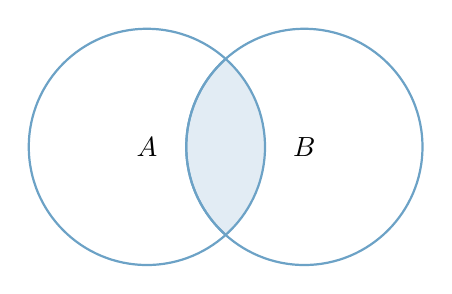
\begin{tikzpicture}
        % Use clipping to shade only the intersection
        \begin{scope}
            \clip \firstcircle;
            \fill[filled] \secondcircle;
        \end{scope}
        
        % Draw the outlines on top for a clean look
        \draw[outline] \firstcircle node {$A$};
        \draw[outline] \secondcircle node {$B$};
    \end{tikzpicture}
    \caption{The shaded region represents the intersection $A \cap B$.}
    \label{fig:intersection_custom}
\end{figure}

\subsection*{Union}
The union of two sets contains all the elements that appear in either set (or both). It corresponds to the logical \texttt{OR} operator.

\begin{definition}[Union]
    The \textbf{union} of sets $A$ and $B$, denoted $A \cup B$, is the set containing all elements that are in $A$, or in $B$, or in both.
    \[ A \cup B = \{ x \mid x \in A \text{ or } x \in B \} \]
\end{definition}

% --- Union Figure (Your Style) ---
\begin{figure}[htbp]
    \centering
    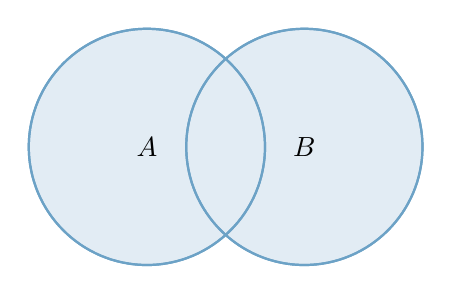
\begin{tikzpicture}
        % Fill both circles
        \fill[filled] \firstcircle \secondcircle;
        
        % Draw the outlines on top
        \draw[outline] \firstcircle node {$A$};
        \draw[outline] \secondcircle node {$B$};
    \end{tikzpicture}
    \caption{The shaded region represents the union $A \cup B$.}
    \label{fig:union_custom}
\end{figure}

\subsection*{Set Difference}
The difference between two sets contains the elements that are in the first set but \textit{not} in the second set.

\begin{definition}[Set Difference]
    The \textbf{difference} of set $A$ and set $B$, denoted $A \setminus B$, is the set containing all elements that are in $A$ but not in $B$.
    \[ A \setminus B = \{ x \mid x \in A \text{ and } x \notin B \} \]
\end{definition}

% --- Set Difference Figure (Your Style) ---
\begin{figure}[htbp]
    \centering
    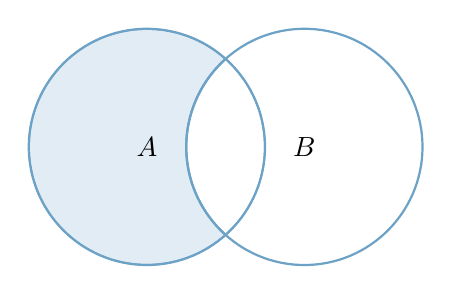
\begin{tikzpicture}
        % Use clip and even-odd rule to shade A without the intersection
        \begin{scope}
            \clip \firstcircle;
            \fill[filled, even odd rule] \firstcircle \secondcircle;
        \end{scope}
        
        % Draw the outlines on top
        \draw[outline] \firstcircle node {$A$};
        \draw[outline] \secondcircle node {$B$};
    \end{tikzpicture}
    \caption{The shaded region represents the difference $A \setminus B$.}
    \label{fig:difference_custom}
\end{figure}

\subsection*{Symmetric Difference}
The symmetric difference contains all elements that are in one set or the other, but not in both. It corresponds to the logical \texttt{XOR} operator.

\begin{definition}[Symmetric Difference]
    The \textbf{symmetric difference} of sets $A$ and $B$, denoted $A \oplus B$, is the set of elements which are in either of the sets, but not in their intersection.
    \[ A \oplus B = (A \cup B) \setminus (A \cap B) \]
\end{definition}

% --- Symmetric Difference Figure (Your Style) ---
\begin{figure}[htbp]
    \centering
    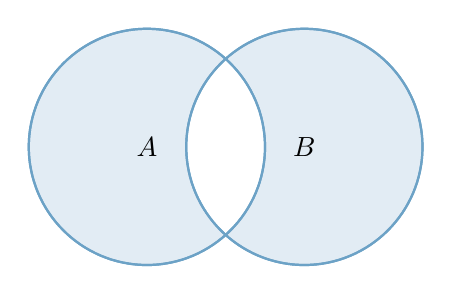
\begin{tikzpicture}
        % Use the even-odd rule to fill the non-overlapping parts
        \fill[filled, even odd rule] \firstcircle \secondcircle;
        
        % Draw the outlines on top
        \draw[outline] \firstcircle node {$A$};
        \draw[outline] \secondcircle node {$B$};
    \end{tikzpicture}
    \caption{The shaded region represents the symmetric difference $A \oplus B$.}
    \label{fig:symmetric_difference_custom}
\end{figure}

\subsection*{Complement}
The complement of a set contains all the elements in the universal set that are \textit{not} in the set itself. It corresponds to the logical \texttt{NOT} operator.

\begin{definition}[Complement]
    The \textbf{complement} of a set $A$, denoted $A^c$, is the set of all elements in the universal set $U$ that are not in $A$.
    \[ A^c = U \setminus A \]
\end{definition}

% --- Complement Figure (Your Style) ---
\begin{figure}[htbp]
    \centering
    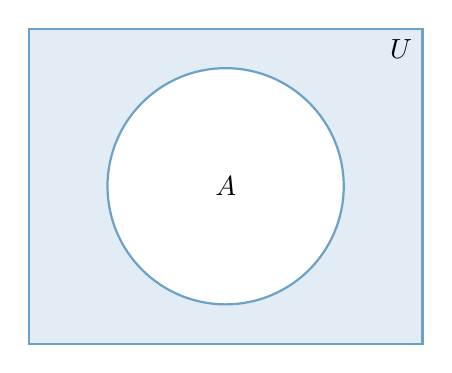
\begin{tikzpicture}
        % Draw and fill the universal set
        \fill[filled] (-2.5, -2) rectangle (2.5, 2);
        
        % "Erase" the circle by filling it with white
        \fill[white] \firstcircle;
        
        % Draw outlines on top
        \draw[outline] (-2.5, -2) rectangle (2.5, 2) node[below left] {$U$};
        \draw[outline] \firstcircle node {$A$};
    \end{tikzpicture}
    \caption{The shaded region represents the complement $A^c$.}
    \label{fig:complement_custom}
\end{figure}

%======================================================================
% SECTION: Cartesian Products and Tuples
%======================================================================
\section{Cartesian Products and Tuples}
While sets are unordered collections, we often need to work with ordered collections in computer science, such as coordinates, database records, or structured data. The Cartesian product is the set operation that allows us to create these ordered structures.

\subsection*{Cartesian Product}
The Cartesian product creates a new set from two or more existing sets, consisting of all possible ordered combinations of their elements.

\begin{definition}[Cartesian Product]
    The \textbf{Cartesian product} of sets $A$ and $B$, denoted $A \times B$, is the set of all possible ordered pairs $(a, b)$, where the first element $a$ is from $A$ and the second element $b$ is from $B$.
    \[ A \times B = \{ (a, b) \mid a \in A \text{ and } b \in B \} \]
\end{definition}

The name comes from the Cartesian coordinate system, where any point on a 2D plane can be represented by an ordered pair $(x, y)$ from the Cartesian product of the real numbers, $\mathbb{R} \times \mathbb{R}$.

% --- Cartesian Product Figure ---
\begin{figure}[htbp]
    \centering
    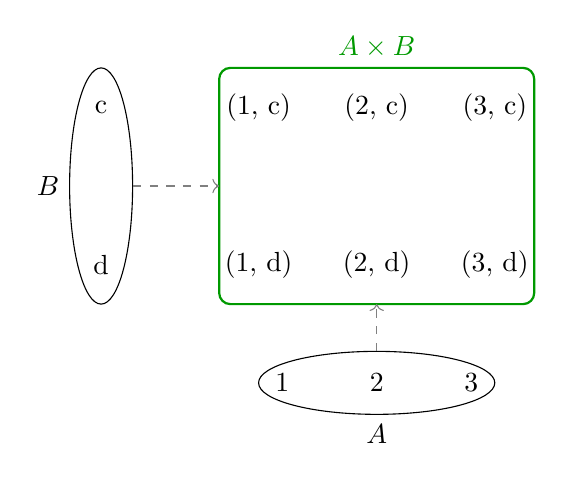
\begin{tikzpicture}[
        setA/.style={ellipse, draw, minimum width=3cm, minimum height=0.8cm},
        setB/.style={ellipse, draw, minimum width=0.8cm, minimum height=3cm},
        element/.style={circle, fill, inner sep=1.5pt}
    ]
        % Set A
        \node[setA, label=below:$A$] (A) at (3.5, -2.5) {};
        \node at (2.3, -2.5) {1};
        \node at (3.5, -2.5) {2};
        \node at (4.7, -2.5) {3};
        
        % Set B
        \node[setB, label=left:$B$] (B) at (0, 0) {};
        \node at (0, 1) {c};
        \node at (0, -1) {d};
        
        % Product Grid
        \draw[thick, green!60!black, rounded corners] (1.5, -1.5) rectangle (5.5, 1.5);
        \node[above, green!60!black] at (3.5, 1.5) {$A \times B$};
        
        % Grid elements
        \node at (2, 1) {(1, c)};
        \node at (3.5, 1) {(2, c)};
        \node at (5, 1) {(3, c)};
        \node at (2, -1) {(1, d)};
        \node at (3.5, -1) {(2, d)};
        \node at (5, -1) {(3, d)};
        
        % Connecting lines (optional)
        \draw[->, gray, dashed] (A.north) -| (3.5, -1.5);
        \draw[->, gray, dashed] (B.east) |- (1.5, 0);
    \end{tikzpicture}
    \caption{The Cartesian product of $A=\{1,2,3\}$ and $B=\{c,d\}$ results in a set of 6 ordered pairs.}
    \label{fig:cartesian_product}
\end{figure}

\begin{remark}
    The order of the sets in a Cartesian product matters. The set $A \times B$ is generally not equal to the set $B \times A$. For example, the pair $(1, c)$ is in $A \times B$, but the pair $(c, 1)$ would be in $B \times A$.
\end{remark}

\subsection*{Tuples}
The elements of a Cartesian product are called \textbf{tuples}. If the product involves $n$ sets, its elements are called \textbf{n-tuples}.

\begin{itemize}
    \item A \textbf{2-tuple}, such as $(a, b)$, is more commonly known as an \textbf{ordered pair}.
    \item A \textbf{3-tuple} has the form $(a, b, c)$.
    \item An \textbf{n-tuple} has the form $(a_1, a_2, \dots, a_n)$.
\end{itemize}

The defining characteristic of a tuple is that \textbf{order matters}. This makes tuples fundamentally different from sets.
\begin{itemize}
    \item For sets: $\{1, 2, 3\} = \{3, 2, 1\}$
    \item For tuples: $(1, 2, 3) \neq (3, 2, 1)$
\end{itemize}
This property makes tuples ideal for representing data where the position of an element carries meaning, such as a database record `(UserID, Name, Email)`.

%======================================================================
% SECTION: Proving Set Equalities
%======================================================================
\section{Proving Set Equalities}
In software development, simplifying complex conditional logic is crucial for writing efficient and readable code. Similarly, in set theory, we often need to prove that two different expressions describe the exact same set. There are two primary methods for this: using membership tables and applying set identities.

\subsection*{Method 1: Membership Tables}
A membership table is a tool used to prove that two set expressions are equal by checking every possible combination of an element's membership in the constituent sets.

This method is the set-theory equivalent of using a \textbf{truth table} in Boolean algebra. Instead of checking for \texttt{TRUE} or \texttt{FALSE}, we check if an element is a member (represented by a $1$) or not a member (represented by a $0$) of a set. If the columns for two different set expressions are identical in all rows, the expressions are proven to be equal.

\begin{example}{Showing that $A \cap B = B \setminus (B \setminus A)$}\\
    To prove this equality, we construct a membership table for all combinations of membership in sets $A$ and $B$.
    
    \begin{center}
    \renewcommand{\arraystretch}{1.5}
    \begin{tabular}{|c|c||c|c|c|}
        \hline
        $A$ & $B$ & $A \cap B$ & $B \setminus A$ & $B \setminus (B \setminus A)$ \\
        \hline
        1 & 1 & \textbf{1} & 0 & \textbf{1} \\
        1 & 0 & \textbf{0} & 0 & \textbf{0} \\
        0 & 1 & \textbf{0} & 1 & \textbf{0} \\
        0 & 0 & \textbf{0} & 0 & \textbf{0} \\
        \hline
    \end{tabular}
    \end{center}
    \label{ex:membership_table}

\begin{solution} (\autoref{ex:membership_table}) Since the column for $A \cap B$ is identical to the column for $B \setminus (B \setminus A)$ for all possible membership combinations, the two expressions are equal.
\end{solution}

\end{example}



\subsection*{Method 2: Set Identities}
While membership tables are effective, they can become very large as the number of sets increases. A more algebraic approach is to use \textbf{set identities} to simplify one expression until it matches the other. These identities are fundamental laws that govern how set operations behave.

\autoref{tab:set_identities} shows the most important set identities. Notice the striking similarity to the laws of Boolean algebra — they are structurally identical.

% --- Set Identities Table ---
\begin{table}
\centering
\caption{Fundamental Set Identities and their Boolean Algebra Counterparts.}
\label{tab:set_identities}
\renewcommand{\arraystretch}{1.4}
\begin{tabular}{|l|l|l|}
\hline
\textbf{Identity Name} & \textbf{Set Identity} & \textbf{Boolean Identity} \\
\hline
Identity Laws & $A \cup \emptyset = A$ & $x + 0 = x$ \\
& $A \cap U = A$ & $x \cdot 1 = x$ \\
\hline
Domination Laws & $A \cup U = U$ & $x + 1 = 1$ \\
& $A \cap \emptyset = \emptyset$ & $x \cdot 0 = 0$ \\
\hline
Idempotent Laws & $A \cup A = A$ & $x + x = x$ \\
& $A \cap A = A$ & $x \cdot x = x$ \\
\hline
Complement Laws & $A \cup A^c = U$ & $x + \overline{x} = 1$ \\
& $A \cap A^c = \emptyset$ & $x \cdot \overline{x} = 0$ \\
\hline
Commutative Laws & $A \cup B = B \cup A$ & $x + y = y + x$ \\
& $A \cap B = B \cap A$ & $x \cdot y = y \cdot x$ \\
\hline
Associative Laws & $(A \cup B) \cup C = A \cup (B \cup C)$ & $(x+y)+z = x+(y+z)$ \\
& $(A \cap B) \cap C = A \cap (B \cap C)$ & $(x \cdot y) \cdot z = x \cdot (y \cdot z)$ \\
\hline
Distributive Laws & $A \cap (B \cup C) = (A \cap B) \cup (A \cap C)$ & $x \cdot (y+z) = (x \cdot y)+(x \cdot z)$ \\
& $A \cup (B \cap C) = (A \cup B) \cap (A \cup C)$ & $x + (y \cdot z) = (x+y) \cdot (x+z)$ \\
\hline
De Morgan's Laws & $(A \cap B)^c = A^c \cup B^c$ & $\overline{x \cdot y} = \overline{x} + \overline{y}$ \\
& $(A \cup B)^c = A^c \cap B^c$ & $\overline{x + y} = \overline{x} \cdot \overline{y}$ \\
\hline
Absorption Laws & $A \cup (A \cap B) = A$ & $x + (x \cdot y) = x$ \\
& $A \cap (A \cup B) = A$ & $x \cdot (x+y) = x$ \\
\hline
\end{tabular}
\end{table}

\begin{example}{Proving $A \cup (B \cap A^c) = A \cup B$ using identities}
\begin{align*}
    A \cup (B \cap A^c) &= (A \cup B) \cap (A \cup A^c) && \text{by Distributive Law} \\
    &= (A \cup B) \cap U && \text{by Complement Law} \\
    &= A \cup B && \text{by Identity Law}
\end{align*}
\end{example}

\begin{example}{Determine whether $(A \cap B) \cup (A \cap B^c) = A$}
\begin{solution}
Let's simplify the left side using set identities:
\begin{align*}
    (A \cap B) \cup (A \cap B^c) &= A \cap (B \cup B^c) && \text{by Distributive Law} \\
    &= A \cap U && \text{by Complement Law} \\
    &= A && \text{by Identity Law}
\end{align*}
Since the left side simplifies to $A$, we have $(A \cap B) \cup (A \cap B^c) = A$. \textbf{The expressions are equal.}
\end{solution}
\end{example}

\begin{example}{Determine whether $(A \cup B) \cap (A^c \cup B^c) = A \cap B$}
\begin{solution}
Let's simplify the left side:
\begin{align*}
    (A \cup B) \cap (A^c \cup B^c) &= (A \cup B) \cap (A \cap B)^c && \text{by De Morgan's Law} \\
    &= (A \cup B) \cap (A \cap B)^c
\end{align*}
This represents all elements that are in $A$ or $B$ but not in both $A$ and $B$ simultaneously. This is the symmetric difference $A \oplus B$, not $A \cap B$.

For a concrete counterexample, let $A = \{1, 2\}$ and $B = \{2, 3\}$:
\begin{itemize}
    \item $(A \cup B) \cap (A^c \cup B^c) = \{1, 2, 3\} \cap \{3, 1\} = \{1, 3\}$
    \item $A \cap B = \{2\}$
\end{itemize}
Since $\{1, 3\} \neq \{2\}$, \textbf{the expressions are not equal.}
\end{solution}
\end{example}

\begin{example}{Determine whether $A \cup (B \cap C) = (A \cup B) \cap (A \cup C)$}
\begin{solution}
This is actually the Distributive Law for union over intersection. Let's verify:
\begin{align*}
    (A \cup B) \cap (A \cup C) &= A \cup (B \cap C) && \text{by Distributive Law}
\end{align*}
So we have $A \cup (B \cap C) = (A \cup B) \cap (A \cup C)$. \textbf{The expressions are equal.}
\end{solution}
\end{example}

\begin{example}{Determine whether $(A \cap B^c) \cup (A^c \cap B) = (A \cup B) \cap (A \cap B)^c$}
\begin{solution}
The left side is the symmetric difference $A \oplus B$. Let's check the right side:
\begin{align*}
    (A \cup B) \cap (A \cap B)^c &= (A \cup B) \cap (A^c \cup B^c) && \text{by De Morgan's Law} \\
    &= (A \cap A^c) \cup (A \cap B^c) \cup (B \cap A^c) \cup (B \cap B^c) && \text{by Distributive Law} \\
    &= \emptyset \cup (A \cap B^c) \cup (A^c \cap B) \cup \emptyset && \text{by Complement Law} \\
    &= (A \cap B^c) \cup (A^c \cap B) && \text{by Identity Law}
\end{align*}
Since both sides equal $(A \cap B^c) \cup (A^c \cap B)$, \textbf{the expressions are equal.}
\end{solution}
\end{example}



%======================================================================
% SECTION: Computer Representation of Sets
%======================================================================
\section{Computer Representation of Sets}
While set theory provides the abstract language for collections, computer science requires concrete and efficient ways to implement these ideas. For finite universal sets, one of the most elegant and performant methods is to represent sets using \textbf{bit strings}.This technique requires two conditions:
\begin{enumerate}
    \item The universal set $U$ must be finite.
    \item The elements of $U$ must have a fixed, agreed-upon order.
\end{enumerate}

Let $U = \{a_1, a_2, \dots, a_n\}$. Any subset $A \subseteq U$ can be represented by a bit string of length $n$, where the $i$-th bit is $1$ if $a_i \in A$, and $0$ if $a_i \notin A$.

\begin{example}{Representing Sets as Bit Strings}\\
    Let the universal set be $U = \{1, 2, 3, 4, 5, 6, 7, 8\}$.
    \begin{itemize}
        \item The set $A = \{1, 3, 4, 8\}$ is represented by the bit string \texttt{10110001}.
        \item The set $B = \{2, 3, 8\}$ is represented by the bit string \texttt{01100001}.
        \item The set of all even numbers, $\{2, 4, 6, 8\}$, is \texttt{01010101}.
        \item The empty set, $\emptyset$, is \texttt{00000000}.
    \end{itemize}
\end{example}

The true power of this representation is that set operations map directly to extremely fast, low-level bitwise operations that processors can execute in a single cycle.

\begin{custombox}{Set Operations as Bitwise Operations}
    Let the bit strings for sets $A$ and $B$ be $s_A$ and $s_B$.
    \begin{itemize}
        \item \textbf{Union ($A \cup B$)} corresponds to a bitwise \textbf{\texttt{OR}} operation.
        \item \textbf{Intersection ($A \cap B$)} corresponds to a bitwise \textbf{\texttt{AND}} operation.
        \item \textbf{Complement ($A^c$)} corresponds to a bitwise \textbf{\texttt{NOT}} (one's complement) operation.
        \item \textbf{Symmetric Difference ($A \oplus B$)} corresponds to a bitwise \textbf{\texttt{XOR}} operation.
    \end{itemize}
\end{custombox}

\begin{example}Performing Set Operations with Bit Strings\\
    Using $U = \{1, 2, 3, 4, 5, 6, 7, 8\}$, let $A = \{1, 3, 4, 8\}$ and $B = \{2, 3, 8\}$.
    
    \begin{center}
    \renewcommand{\arraystretch}{1.4}
    \begin{tabular}{rll}
         & \textbf{Set Representation} & \textbf{Bit String Representation} \\
        \hline
        Set $A$ & $\{1, 3, 4, 8\}$ & \texttt{10110001} \\
        Set $B$ & $\{2, 3, 8\}$ & \texttt{01100001} \\
        \hline
        $A \cup B$ & $\{1, 2, 3, 4, 8\}$ & \texttt{10110001 OR 01100001 = 11110001} \\
        $A \cap B$ & $\{3, 8\}$ & \texttt{10110001 AND 01100001 = 00100001} \\
        $A^c$ & $\{2, 5, 6, 7\}$ & \texttt{NOT 10110001 = 01001110} \\
    \end{tabular}
    \end{center}
\end{example}

This bit string representation is fundamental in many areas of computing, including file permissions in operating systems, database indexing, network protocols, and graphics programming, as it provides a way to manage and query collections with maximum efficiency.
\chapter{Combinatorics and Probability Theory}
\label{chap:ch4}
Imagine you are tasked with forming teams of 3 for a semester project in a class of 45 students. Initially, the order in which you choose the team members does not matter, so you are just concerned with combinations. The number of ways to form a team of 3 from 45 students comes out to 14,190 possibilities!

The following semester introduces the students to Scrum project management, where each team must have three specific roles: Scrum Master, Product Owner, and Development Team. This small change, specifying roles, suddenly transforms the problem from a simple \textit{combination} into a \textit{permutation}. Now, the number of possible ways to assign these roles leaps to 85,140!

Frustrated by the sheer number of options, the 45 students throw a party to relax. Being well-mannered, they decide that everyone should shake hands with every other person exactly once. After a few minutes, they calculate the total number of handshakes — 990. The students are once again surprised by how something as simple as shaking hands can add up so quickly.

As the night progresses, one student proposes a fun game — a random drawing for five door prizes, each unique. With 45 students in attendance and only five prizes available, the chance of winning nothing becomes a concerning 89 per cent. The students quickly realize that the odds are not in their favor.

Not ready to give up on their luck, a smaller group decides to flip a coin 10 times, with the hope of landing exactly five heads to win the game. However, when they learn that the probability of this happening is only about 25 per cent, their spirits dampen further.

The students conclude that rather than relying on chance, it is time to dive deeper into understanding combinatorics and probability theory. Armed with this knowledge, they can better predict outcomes and avoid future disappointments at both parties and project planning.

\section{Sample Space and Events}
\label{sec:sample_space}
A \textbf{random experiment }is one that can lead to different outcomes, even when repeated under the same conditions. This randomness is a fundamental aspect of many engineering tasks.

Think of it this way: Let us say you are testing the speed of a website under different conditions. Sometimes it loads quickly, and other times it is slower. Even if you are using the same code and server, things like network traffic or server load make the results vary each time. 

\begin{definition}{Random Experiment}
    A random experiment is one that can give different results, even if you do everything the same each time.
\end{definition}

Or, imagine you are measuring the signal strength in a wireless device. You might get slightly different readings each time because of things like interference or small changes in the environment.

This randomness shows up all over the place, from software performance tests to electrical engineering experiments. It is important to expect it and include it in your thinking. Otherwise, you might make decisions based on incomplete or misleading data. When you account for random variation, you can make smarter predictions and designs.

To model and analyze a random experiment, it is crucial to understand the set of possible outcomes that can occur. In probability theory, this set is called the \textbf{sample space}, denoted by \( S \). A sample space can be either \textbf{discrete} (consisting of a finite or countably infinite set of outcomes) or \textbf{continuous} (containing an interval of real numbers). The exact definition of a sample space often depends on the objectives of the analysis.

An \textbf{outcome} is a single possible result of the random experiment, and an \textbf{event} is any subset of the sample space, which may consist of one or more outcomes. Below are some examples to illustrate these concepts:

\begin{example}[ Network Latency] \\
Consider an experiment where you measure the latency of data packets in a network. The sample space can be defined based on the type of measurements:
\begin{itemize}
    \item If latency is measured as a positive real number, the sample space is continuous: 
    \[
    S = \{ x \mid x > 0 \}.
    \]
    \item If it is known that latency ranges between 10 and 100 milliseconds, the sample space can be refined to:
    \[
    S = \{ x \mid 10 \leq x \leq 100 \}.
    \]
    \item If the objective is to categorize latency as low, medium, or high, the sample space becomes discrete:
    \[
    S = \{\text{low}, \text{medium}, \text{high}\}.
    \]
    \item For a simple evaluation of whether the latency meets a standard threshold, the sample space can be reduced to:
    \[
    S = \{\text{pass}, \text{fail}\}.
    \]
\end{itemize}
Each outcome in these sample spaces represents a single possible latency measurement, and events can be defined as sets of outcomes, such as "latency is high."

\end{example}

Understanding the nature of sample spaces, outcomes, and events is fundamental in probability, as it allows us to define and work with probabilities of complex scenarios in various engineering contexts. Let us summarise these key concepts:

\begin{definition}{Sample Spaces, Outcomes, and Events}
    \textbf{Sample Space:} The set of all possible outcomes of a random experiment is called the sample space, denoted by \( S \). Outcomes can be discrete or continuous, depending on the nature of the experiment.
    
    \textbf{Outcome:} A single possible result of a random experiment.
    
    \textbf{Event:} Any subset of the sample space, which may consist of one or more outcomes.
\end{definition}

\begin{example} Software Release Testing \\
    Imagine a software testing process where each test case can either pass or fail. The sample space for a single test case is discrete and can be represented as:
    \[
    S = \{\text{pass}, \text{fail}\}.
    \]
    If you run three test cases, the combined sample space for all possible outcomes is:
    \begin{align*}
    S = \{&(\text{pass, pass, pass}), (\text{pass, pass, fail}), (\text{pass, fail, pass}), \\
    &(\text{pass, fail, fail}), (\text{fail, pass, pass}), (\text{fail, pass, fail}), \\
    &(\text{fail, fail, pass}), (\text{fail, fail, fail})\}.
    \end{align*}
    This sample space includes all sequences of outcomes for the three tests.
    
    \begin{itemize}
        \item The total number of possible outcomes is \( 2^3 = 8 \).
        \item An event could be defined as "at least one test fails," which would include outcomes like \(\text{(fail, pass, pass)}\), \(\text{(pass, fail, fail)}\), and others where at least one test fails.
    \end{itemize}
    
    \end{example}
    

\begin{example} Component Quality in Manufacturing \\
A company manufactures electronic components, and each component is tested for compliance with quality standards. The test can return one of three outcomes: \texttt{pass}, \texttt{marginal}, or \texttt{fail}. The sample space is:
\[
S = \{\text{pass}, \text{marginal}, \text{fail}\}.
\]
\textbf{Event:} Suppose we are interested in the event that a component does not pass the quality test. This event is a set of outcomes:
\[
E = \{\text{marginal}, \text{fail}\}.
\]
\end{example}

This means that all the operations we have defined on sets translate directly into operations on events:
\begin{itemize}
    \item $A \cup B$: the event that at least one of $A$ or $B$ occurs.
    \item $A \cap B$: the event that both $A$ and $B$ occur together.
    \item $\skoverline{A}$ or $A^c$: the event that $A$ does not occur.
    \item $A \setminus B$ or $A - B$: the event that $A$ occurs but $B$ does not.
    \item $A \Delta B$ or $A \oplus B$: the event that either $A$ or $B$ occurs, but not both (symmetric difference).
\end{itemize}

Thus, probability theory builds directly on set theory: probability assigns a numerical measure to these subsets of the sample space. In the next chapter, we will see how this measure is defined and used to reason about uncertainty.

We can summarise the considerations of this section in the following table:

\begin{table}[h]
    \centering
    \renewcommand{\arraystretch}{1.5} % Adjust this value for desired spacing
    \begin{tabular}{|c|c|c|c|}
    \hline
    \textbf{Operation} & \textbf{Boolean Algebra} & \textbf{Logic} & \textbf{Set Theory} \\
    \hline
    \texttt{NOT} & $\skoverline{x}$ & $\neg x$ & $A^c$ or $A'$\\
    \hline
    \texttt{OR} & $+$ & $\vee$ & $\cup$ \\
    \hline
    \texttt{AND} & $\cdot$ & $\wedge$ & $\cap$ \\
    \hline
    \texttt{NAND} & $\skoverline{x \cdot y}$ & $\neg (x \wedge y)$ & $(A \cap B)^c$ or \(\skoverline{A \cap B}\)\\
    \hline
    \texttt{NOR} & $\skoverline{x + y}$ & $\neg (x \vee y)$ & $(A \cup B)^c$ or \(\skoverline{A \cup B}\) \\
    \hline
    \texttt{XOR} (Symmetric Difference) & $x \oplus y$ & $(x \wedge \neg y) \vee (\neg x \wedge y)$ & $A \triangle B$ or \(A \oplus B\) \\
    \hline
    Difference & $x \cdot \skoverline{y}$ & $x \wedge \neg y$ & $A - B$ or \( A \setminus B \) \\
    \hline
    \end{tabular}
    \caption{Comparison of Operators in Boolean Algebra, Logic, and Set Theory}
\end{table}

In this book, we will use the notation $A^c$ to denote the complement of the set $A$, which includes all elements not in $A$.

\section{Counting Principles}

In many problems across mathematics, computer science, and engineering, determining the number of ways certain events can occur is important. Whether you're arranging elements, selecting groups, or navigating through complex scenarios, counting techniques provide the foundational tools to solve these problems. These techniques go beyond simple arithmetic and allow us to tackle questions like:

\begin{itemize}
    \item How many ways can we arrange a set of objects?
    \item In how many different paths can a process unfold?
    \item What is the probability of a specific event occurring given multiple possibilities?
\end{itemize}

Counting techniques, such as permutations, combinations, and the multiplication rule, help us quantify these possibilities systematically.

\subsection*{Multiplication Rule}

We start out by discussing the most basic counting principle: the \textbf{multiplication rule}:

\begin{theorem}[Multiplication Rule]
    Let an operation be described as a sequence of $k$ steps. Assume the following conditions:
    
    \begin{itemize}
        \item There are $n_1$ ways to complete step 1.
        \item There are $n_2$ ways to complete step 2 for each way of completing step 1.
        \item There are $n_3$ ways to complete step 3 for each way of completing step 2, and so on.
    \end{itemize}
    
    Then, the total number of ways to complete the entire operation is given by:
    
    \[
    n_1 \times n_2 \times \cdots \times n_k.
    \]
\end{theorem}
    
\begin{example}
    Suppose you are choosing a meal at a restaurant. You have the following options:
        
    \begin{itemize}
            \item 3 choices for the main course.
            \item 4 choices for the side dish.
            \item 2 choices for the drink.
    \end{itemize}
        
    Using the multiplication rule, the total number of ways to choose a meal is:
        
    \[
        3 \times 4 \times 2 = 24.
    \]
        
    Therefore, there are 24 different meal combinations available.
\end{example}

\begin{example} Automobile Options

An automobile manufacturer provides vehicles equipped with selected
options. Each vehicle is ordered

\begin{itemize}
    \item With or without an automatic transmission
    \item With or without a sunroof
    \item With one of three choices of a stereo system
    \item With one of four exterior colors
\end{itemize}

If the sample space consists of the set of all possible vehicle types, what is the number of outcomes in the sample space?
\end{example}

\begin{solution}
Using the multiplication rule, we can calculate the total number of possible vehicle types by multiplying the number of choices for each option:

\begin{itemize}
    \item 2 choices for the transmission (with or without automatic transmission)
    \item 2 choices for the sunroof (with or without sunroof)
    \item 3 choices for the stereo system
    \item 4 choices for the exterior color
\end{itemize}

Therefore, the total number of possible vehicle types is:

\[
2 \times 2 \times 3 \times 4 = 48
\]

So, there are 48 different possible vehicle types in the sample space.
\end{solution}

\subsection*{Replacement and Order in Counting}

Next we turn to an important distinction between with and without replacement in counting principles:

\begin{definition}[Counting with and without Replacement]
    When counting the number of ways to select objects from a set, two common scenarios are:

    \begin{itemize}
        \item \textbf{With Replacement}: An object can be selected more than once.
        \item \textbf{Without Replacement}: Once an object is selected, it cannot be chosen again.
    \end{itemize}
    \end{definition}
    
\begin{example}
    Suppose you have a bag containing 5 different colored balls. You draw 2 balls:
\begin{itemize}
    \item \textbf{With Replacement}: The first ball is placed back in the bag before drawing the second. There are \(5 \times 5 = 25\) possible outcomes.
    \item \textbf{Without Replacement}: The first ball is not placed back, so the number of outcomes is \(5 \times 4 = 20\).
\end{itemize}
\end{example}

\begin{example}
    Three people are drawing cards one after another from a standard deck of 52 cards. The goal is to find the Ace of Spades. Let's examine the two scenarios: with replacement and without replacement.

    \textbf{Without Replacement}

    In this scenario, each card drawn is not put back into the deck, reducing the total number of cards available after each draw.
    \begin{itemize}
        \item First Draw: The first person has a $\frac{1}{52}$ chance of drawing the Ace of Spades.
        \item Second Draw: If the first person does not draw the Ace of Spades, there are now 51 cards left, and the second person has a $\frac{1}{51}$ chance of drawing the Ace of Spades.
        \item Third Draw: If the Ace of Spades has not been drawn by the first two people, the third person has a $\frac{1}{50}$ chance of drawing it.
    \end{itemize}
    
    The probabilities change with each draw because the total number of cards decreases, and previously drawn cards are not available.
    
    \textbf{With Replacement}

    In this scenario, each card drawn is returned to the deck and reshuffled before the next person draws. This keeps the total number of cards constant.
    \begin{itemize}
        \item First Draw: The first person has a $\frac{1}{52}$ chance of drawing the Ace of Spades.
        \item Second Draw: Since the card is replaced and shuffled back into the deck, the second person also has a $\frac{1}{52}$ chance of drawing the Ace of Spades.
        \item Third Draw: Similarly, the third person has a $\frac{1}{52}$ chance of drawing the Ace of Spades.
    \end{itemize}
    
    The probabilities remain the same for each draw because the deck is reset to its original state after each draw.

\end{example}

\begin{example}
    Imagine you have a group of 5 students: Alice, Bob, Charlie, David, and Eve. You need to select 2 of them for different scenarios, illustrating when the order of selection matters and when it does not.
    \begin{itemize}
        \item \textbf{Order Matters}: Selecting Alice as Captain and Bob as Assistant Captain is a different outcome than selecting Bob as Captain and Alice as Assistant Captain.
        \end{itemize}
    Now, imagine you are simply selecting 2 students to form a study group with no specific roles assigned. Here, the order does not matter.
    \begin{itemize}
        \item \textbf{Order does not matter:}  Choosing Alice and Bob is considered the same outcome as choosing Bob and Alice; there is no distinction between the two orders since there are no assigned roles.
    \end{itemize}
    \label{ex:order_matters}
\end{example}

\autoref{ex:order_matters} illustrates the distinction between \textit{permutations} and \textit{combinations}, two fundamental counting principles that are widely used in probability theory and combinatorics.

\begin{definition}[Permutation and Combination]
    \begin{itemize}
        \item \textbf{Permutation (order matters)}: Different sequences are counted as distinct outcomes, leading to a higher count.
        \item \textbf{Combination (order does not matter)}: Sequences are treated as identical, resulting in a lower count.
    \end{itemize}
\end{definition}

We will first discuss permutations, which are used when the order of selection matters.

\subsection*{Permutations}

Consider a set of elements, such as $S=\{a, b, c\}$. A permutation of the elements is an ordered sequence of the elements. For example, $a b c, a c b, b a c, b c a, c a b$, and $c b a$ are all the permutations of the elements of $S$.

\begin{proposition}[Permutations of \(n\) Distinct Objects]
    The number of ordered arrangements (permutations) of $n$ distinct objects is
    \[
    n! = n \cdot (n-1) \cdot \dots \cdot 2 \cdot 1.
    \]
\end{proposition}

This outcome is a direct application of the multiplication rule. To form a permutation, you start by choosing an element for the first position from the total of $n$ elements. Next, you choose an element for the second position from the remaining $n-1$ elements, then for the third position from the remaining $n-2$ elements, and continue this way until all positions are filled. Such arrangements are often called linear permutations.

\begin{example}
    It is said that any shuffling of a deck of card has only happened once in history. This is because the number of ways to shuffle a deck of 52 cards is \(52!\), which is an astronomically large number.

    \[52! \approx 8.07 \times 10^{67}\]
\end{example}

\begin{example}
    Suppose you have 5 different books on a shelf. You want to rearrange them in a different order. The number of ways to rearrange the books is
    \[5! = 5 \times 4 \times 3 \times 2 \times 1 = 120\]
\end{example}

There are cases where we are only interested in arranging a subset of elements from a larger set. The formula for counting these arrangements also derives from the multiplication rule.

\begin{theorem}[Permutations of Subsets]
    For integers $n \ge r \ge 0$, the number of ordered selections of $r$ distinct objects from $n$ distinct objects is
    \[
    P_r^n = P(n,r) = n \cdot (n-1) \cdots (n-r+1) = \frac{n!}{(n-r)!}.
    \]
\end{theorem}

\begin{example}
    Suppose you have 5 different books on a shelf, and you want to rearrange 3 of them in a different order. The number of ways to rearrange the 3 books is
    \[
    P_3^5=5 \times 4 \times 3 = 60
    \]
\end{example}

\begin{example}
    There are 10 entries in a contest. Only three will win, $1^{\text {st }}, 2^{\text {nd }}$, or $3^{\text {rd }}$ prize. What are the possible results?
\end{example}
\begin{solution}
    The number of ways to award the prizes is the number of permutations of 3 objects selected from 10, which is
    \[
    P_3^{10}= \frac{10!}{(10-3)!}=\frac{10!}{7!} = 10 \times 9 \times 8 = 720
    \]
    Therefore, there are 720 possible outcomes for awarding the prizes.
\end{solution}

\subsection*{Combinations}

When the order of selection does not matter, we use the concept of combinations. Combinations are used when we are interested in selecting a subset of elements from a larger set without regard to the order in which they are selected. Let us start out with a couple of examples to illustrate the concept of combinations.

\begin{example}
    Suppose you have a group of 5 students: Alice, Bob, Charlie, David, and Eve. You need to select 2 of them to form a study group. The order in which you select the students does not matter. The possible combinations are:
    \begin{itemize}
        \item Alice and Bob
        \item Alice and Charlie
        \item Alice and David
        \item Alice and Eve
        \item Bob and Charlie
        \item Bob and David
        \item Bob and Eve
        \item Charlie and David
        \item Charlie and Eve
        \item David and Eve
    \end{itemize}
    The order of the students in the study group does not matter, so the combinations are considered identical.
\end{example}

\begin{example}
    Maria has three tickets for a concert. She'd like to use one of the tickets herself. She could then offer the other two tickets to any of four friends (Ann, Beth, Chris, Dave). How many ways can 2 people be selected from 4 to go to a concert?
\end{example}

\begin{example}
A circuit board has four different locations in which a component can be placed. If three identical components are to be placed on the board, how many different designs are possible?
\end{example}

\begin{solution}
    Since you can only place one component in each slot, placing a component in any slot immediately restricts the choices for the next component.
        
    \begin{enumerate}
        \item Fill slots 1, 2, and 3.
        \item Fill slots 1, 2, and 4.
        \item Fill slots 1, 3, and 4.
        \item Fill slots 2, 3, and 4.
    \end{enumerate}
\end{solution}

These examples illustrate the concept of combinations, where the order of selection does not matter. The formula for combinations is derived from the permutation formula by dividing out the number of ways to arrange the $r$ elements.

\begin{theorem}[Combinations]
    The number of combinations of $r$ elements selected from a set of $n$ different elements is given by
    \[
    C_r^n = \binom{n}{r} = \frac{n!}{r!(n-r)!}
    \]
\end{theorem}

This is also sometimes referred to as the \textbf{binomial coefficient}, denoted by $\binom{n}{r}$, which is read as "n choose r". It is called the binomial coefficient because it appears in the binomial theorem, which expands the powers of a binomial expression:

\begin{theorem}[Binomial Theorem]
    In algebra, the binomial coefficient is used to expand powers of binomials. According to the binomial theorem

$$
(a+b)^n=\sum_{k=0}^n\binom{n}{k} a^k b^{n-k}
$$

\end{theorem}

The theorem states that the expansion of the binomial expression $(a+b)^n$ is the sum of the terms $\binom{n}{k} a^k b^{n-k}$ for $k=0,1,2,\ldots,n$. The binomial coefficient $\binom{n}{k}$ gives the number of ways to choose $k$ elements from a set of $n$ elements. We will place no more emphasis on the binomial theorem here, but it is a fundamental concept in algebra and combinatorics, and is widely used in probability theory.

We will conclude our discussion of counting principles with principles of counting with replacement.

\begin{proposition}[With replacement]
For selections from $n$ types:
\begin{itemize}
    \item \textbf{Ordered with replacement}: $n^r$ outcomes.
    \item \textbf{Unordered with replacement}: $\displaystyle \binom{n+r-1}{r}$ outcomes. % (stars and bars)
\end{itemize}
\end{proposition}

\section{Basic Probability}
Probability quantifies the likelihood or chance that an outcome of a random experiment will occur. For instance, when you hear, “The chance of rain today is 30\%,” it expresses our belief about the likelihood of rain. Probabilities are numbers assigned to outcomes, ranging from 0 to 1 (or equivalently, from 0\% to 100\%). A probability of 0 means the outcome will not happen, while a probability of 1 means it will happen for sure.

Probabilities can be interpreted in different ways:

\begin{itemize}
    \item \textbf{Objective (or Classical) Probability}: Often referred to as classical probability, this approach is used when outcomes are equally likely, such as in rolling a fair die or flipping a coin. Probabilities are assigned based on the assumption that each outcome has an equal chance of occurring. For example, when rolling a fair six-sided die, the probability of rolling a 3 is \( \frac{1}{6} \) because there are 6 equally likely outcomes (1, 2, 3, 4, 5, 6), and only one of them is a 3. The probability is the same for all observers.
        
    \item \textbf{Relative Frequency (Empirical Probability)}: Empirical probability is based on observations from experiments rather than theoretical calculations. For example, if a software tester runs a stress test on a server 100 times, and it crashes 7 times, the empirical probability of a crash is \( \frac{7}{100} = 0.07 \). This approach relies on actual data rather than assumptions or intuition.
        
    \item \textbf{Subjective Probability}: This reflects our personal belief or degree of confidence in an outcome. Different people might assign different probabilities to the same event based on their knowledge or perspective. You and your friends discuss Denmark’s chances of winning the World Cup. Based on recent performance and team strength, you estimate a 10\% chance. However, a more optimistic friend assigns a 20\% chance, while another gives only 5\%, considering stronger competitors. This illustrates subjective probability, where each person's estimate varies based on personal beliefs and biases rather than objective data.
    

\end{itemize}

When assigning probabilities, it’s essential that the sum of all probabilities in an experiment equals 1, ensuring consistency with the relative frequency interpretation.

We start by establishing the Axioms of Probability, which lay the foundation for how probabilities are assigned to events. These axioms define the basic properties that every probability measure must satisfy.
    
\begin{axiom}[Axioms of Probability]
    \begin{itemize}
        \item \textbf{Axiom 1:} For any event \(A\), \( 0 \leq P(A) \leq 1 \).
        \item \textbf{Axiom 2:} Probability of the sample space \(S\) is \(P(S) = 1\).
        \item \textbf{Axiom 3:} If \(A_1, A_2, A_3, \cdots\) are disjoint events, then \(P\left(A_1 \cup A_2 \cup A_3 \cdots\right) = P\left(A_1\right) + P\left(A_2\right) + P\left(A_3\right) + \cdots\)
    \end{itemize}
\end{axiom}

The property that \( 0 \leq P(A) \leq 1 \) is equivalent to the requirement that a relative frequency must be between 0 and 1. The property that \( P(S) = 1 \) is a consequence of the fact that an outcome from the sample space occurs on every trial of an experiment. Consequently, the relative frequency of \( S \) is 1. Property 3 implies that if the events \( A_1 \) and \( A_2 \) have no outcomes in common, the relative frequency of outcomes in \( A_1 \cup A_2 \) is the sum of the relative frequencies of the outcomes in \( A_1 \) and \( A_2 \).

In the next sections we will see more about the probability of events and how to calculate them.

\subsection*{Probability of an Event}
The probability of an event is a measure of the likelihood that the event will occur. It is denoted by \( P(A) \), where \( A \) is the event. The probability of an event ranges from 0 to 1, where 0 indicates that the event will not occur, and 1 indicates that the event will occur for sure.

\begin{definition}[Probability of an Event]
    The probability of an event \( A \), denoted by \( P(A) \), is the likelihood that event \( A \) will occur. It is defined as the ratio of the number of favorable outcomes to the total number of outcomes in the sample space.
    \[
    P(A) = \frac{\text{Number of favorable outcomes}}{\text{Total number of outcomes}}
    \]
\end{definition}

\begin{example}
    Suppose you are testing a software module with 10 different test cases. Out of these, 3 test cases are known to fail due to a bug. If you randomly select one test case to run, what is the probability that the selected test case will fail?
\end{example}

\begin{solution}
    Here, the event $A$ is "the test case fails."
\begin{itemize}
    \item Number of favorable outcomes (failing test cases) $=3$
    \item Total number of outcomes (total test cases) $=10$
\end{itemize}

Using the formula:

$$
P(A)=\frac{\text { Number of favorable outcomes }}{\text { Total number of outcomes }}=\frac{3}{10}=0.3
$$


Therefore, the probability that a randomly selected test case will fail is 0.3 , indicating that there is a $30 \%$ chance of failure.

\end{solution}

\begin{example}
    Imagine a software development environment where you have 50 files, consisting of 20 Python scripts, 15 Java files, and 15 configuration files. If you randomly select one file to edit, what is the probability that the file is a Python script?
\end{example}

\begin{solution}
Here, the event $A$ is "the selected file is a Python script."
\begin{itemize}
    \item Number of favorable outcomes (Python scripts) $=20$
    \item Total number of outcomes (total files) $=50$
\end{itemize}

Using the formula:

$$
P(A)=\frac{\text { Number of favorable outcomes }}{\text { Total number of outcomes }}=\frac{20}{50}=0.4
$$

Thus, the probability of selecting a Python script is 0.4 , meaning there is a $40 \%$ chance of choosing a Python file from the set.

\end{solution}

\section{Probability of Joint Events and Set Operations}
Joint events are formed by applying basic set operations to individual events. Commonly, we encounter unions of events, such as $A \cup B$; intersections of events, such as $A \cap B$; and complements of events, such as $A^c$. These combined events are often of particular interest, and their probabilities can frequently be derived from the probabilities of the individual events that compose them. Understanding these set operations is essential for accurately calculating the probability of joint events. In this section, we will explore how unions of events and other set operations can be used to determine the probabilities of more complex events.

When dealing with events, the intersection represents \texttt{AND} while the union represents \texttt{OR} The probability of the intersection of events $A$ and $B$, denoted as $P(A \cap B)$, can also be expressed as $P(A, B)$ or $P(A B)$.

From the axioms of probability, we can derive the following rules of probabilities:

\begin{theorem}{Rules of Probability}
    \begin{itemize}
        \item \textbf{Complement Rule:} The probability of the complement of event $A$ is
    
        \[
        P(A^c) = 1 - P(A)
        \]

        \item \textbf{Empty Set Rule:} The probability of the empty set is 0, i.e.,
        
        \[P(\emptyset) = 0\]
        
        \item \textbf{Addition Rule:} For any two events $A$ and $B$, the probability of the union of events $A$ and $B$ is given by
        \[
        P(A \cup B) = P(A) + P(B) - P(A \cap B)
        \]

        \item \textbf{Difference Rule:} The probability of the difference between events $A$ and $B$ is given by
        \[
        P(A-B)=P(A)-P(A \cap B)
        \]
        \item \textbf{Subset Rule:} If $A$ is a subset of $B$ ($A \subset B$), then
        \[P(A) \leq P(B)\].
    \end{itemize}
\end{theorem}

We can obtain the Complement Rule by noting:

\begin{align*}
    1 &= P(S) & \text{(axiom 2)} \\
      &= P(A \cup A^c) & \text{(definition of complement)} \\
      &= P(A) + P(A^c) & \text{(since } A \text{ and } A^c \text{ are disjoint)}
\end{align*}

Since $\emptyset=S^c$, we can apply part the Complement Rule to deduce that $P(\emptyset)=1-P(S)=0$. This is intuitive because, by definition, an event occurs when the outcome of the random experiment is part of that event. However, since the empty set contains no elements, no outcome of the experiment can ever belong to it, making its probability zero.

The Difference Rule can be obtained by showing that $P(A)=P(A \cap B)+P(A-B)$. Note that the two sets $A \cap B$ and $A-B$ are disjoint and their union is $A$. Thus, by the third axiom of probability

\begin{align*}
    P(A) &= P\left((A \cap B) \cup (A - B)\right) & \text{(since } A = (A \cap B) \cup (A - B)) \\
         &= P(A \cap B) + P(A - B) & \text{(since } A \cap B \text{ and } A - B \text{ are disjoint)}
    \end{align*}
    

The Addition Rule we obtain by noting that $A$ and $B-A$ are disjoint sets and their union is $A \cup B$. Thus,

\begin{align*}
    P(A \cup B) &= P(A \cup (B - A)) && (\text{since } A \cup B = A \cup (B - A)) \\
                &= P(A) + P(B - A) && (\text{since } A \text{ and } B - A \text{ are disjoint}) \\
                &= P(A) + P(B) - P(A \cap B) && (\text{by part the Difference Rule})
    \end{align*}
    
And finally the Subset Rule is a direct consequence of the fact that if $A \subset B$, then $B$ can be written as the union of $A$ and $B-A$. Since $A$ and $B-A$ are disjoint, we have $P(B)=P(A)+P(B-A) \geq P(A)$.

We conclude this section with a few examples illustrating the application of these rules to calculate probabilities of joint events.

\begin{example}
    A company has bid on two large construction projects. The company president believes that the probability of winning the first contract is 0.6, the probability of winning the second contract is 0.4, and the probability of winning both contracts is 0.2.

    \begin{enumerate}[label=(\alph*)]
        \item What is the probability that the company wins at least one contract?
        \item What is the probability that the company wins the first contract but not the second contract?
        \item What is the probability that the company wins neither contract?
        \item What is the probability that the company wins exactly one contract?
    \end{enumerate}
\end{example}

\begin{solution}
    Let $A$ be the event that the company wins the first contract, and $B$ be the event that the company wins the second contract. Given:
    \begin{itemize}
        \item $P(A) = 0.6$
        \item $P(B) = 0.4$
        \item $P(A \cap B) = 0.2$
    \end{itemize}
    
    \begin{enumerate}[label=(\alph*)]
        \item The probability that the company wins at least one contract is the probability of the union of events $A$ and $B$. Using the Addition Rule:
        
        \begin{align*}
            P(A \cup B) &= P(A) + P(B) - P(A \cap B) \\
                        &= 0.6 + 0.4 - 0.2 \\
                        &= 0.8
        \end{align*}
        
        Therefore, the probability that the company wins at least one contract is 0.8.
        
        \item The probability that the company wins the first contract but not the second contract is the probability of the difference between events $A$ and $B$. Using the Difference Rule:
        
        \begin{align*}
            P(A - B) &= P(A) - P(A \cap B) \\
                    &= 0.6 - 0.2 \\
                    &= 0.4
        \end{align*}
        
        Therefore, the probability that the company wins the first contract but not the second contract is 0.4.
        
        \item The probability that the company wins neither contract is the probability of the complement of the union of events $A$ and $B$. Using the Complement Rule:
        
        \begin{align*}
            P((A \cup B)^c) &= 1 - P(A \cup B) \\
                                    &= 1 - 0.8 \\
                                    &= 0.2
        \end{align*}
        
        Therefore, the probability that the company wins neither contract is 0.2.
        
        \item The probability that the company wins exactly one contract is the probability of the difference between the union of events $A$ and $B$ and the intersection of events $A$ and $B$. Using the Difference Rule:
            
            \begin{align*}
                P((A \cup B) - (A \cap B)) &= P(A \cup B) - P(A \cap B) \\
                                            &= 0.8 - 0.2 \\
                                            &= 0.6
            \end{align*}
            So, the probability that the company wins exactly one contract is 0.6.
            \end{enumerate}
\end{solution}

\begin{example}
    \begin{itemize}
    \item There is a 60 percent chance that it will rain today.
    \item There is a 50 percent chance that it will rain tomorrow.
    \item There is a 30 percent chance that it does not rain either day.
    \end{itemize}
    
\begin{enumerate}[label=(\alph*)]
    \item The probability that it will rain today or tomorrow
    \item The probability that it will rain today and tomorrow.
    \item The probability that it will rain today but not tomorrow.
    \item The probability that it either will rain today or tomorrow, but not both.
\end{enumerate}
    
\begin{solution}
\begin{enumerate}[label=(\alph*)]
    \item     Let \( A \) be the event that it rains today, and \( B \) be the event that it rains tomorrow.
        
    Given:
    \begin{align*}
        P(A \cup B) &= 1 - P\left((A \cup B)^c\right) \quad &\text{by the Complement Rule} \\
                &= 1 - P\left(A^c \cap B^c\right) \quad &\text{by De Morgan's Law} \\
                &= 1 - 0.3 \\
                &= 0.7
    \end{align*}
            
        
    Therefore, the probability that it will rain today or tomorrow is \( 0.7 \).

    \item The probability that it will rain today and tomorrow: this is $P(A \cap B)$. To find this we note that
    \begin{align*}
    P(A \cap B) &= P(A) + P(B) - P(A \cup B) \\
                &= 0.6 + 0.5 - 0.7 \\
                &= 0.4
    \end{align*}

    \item The probability that it will rain today but not tomorrow: this is $P\left(A \cap B^c\right)$.

    \begin{align*}
        P(A \cap B^c) &= P(A - B) \\
                      &= P(A) - P(A \cap B) \\
                      &= 0.6 - 0.4 \\
                      &= 0.2
        \end{align*}
        
    \item The probability that it either will rain today or tomorrow but not both: this is $P(A-B)+P(B-A)$. We have already found $P(A-B)=.2$. Similarly, we can find $P(B-A)$:
    
    \begin{align*}
        P(B-A) & =P(B)-P(B \cap A) \\
        & =0.5-0.4 \\
        & =0.1
        \end{align*}
    Thus,
    \begin{align*}
        P(A-B)+P(B-A) &= 0.2+0.1 \\
                      &= 0.3
    \end{align*}
\end{enumerate}
\end{solution}
\end{example}

\chapter{Combinatorics and Probability Theory}
\label{chap:ch5}
Imagine you are tasked with forming teams of 3 for a semester project in a class of 45 students. Initially, the order in which you choose the team members does not matter, so you are just concerned with combinations. The number of ways to form a team of 3 from 45 students comes out to 14,190 possibilities!

The following semester introduces the students to Scrum project management, where each team must have three specific roles: Scrum Master, Product Owner, and Development Team. This small change, specifying roles, suddenly transforms the problem from a simple \textit{combination} into a \textit{permutation}. Now, the number of possible ways to assign these roles leaps to 85,140!

Frustrated by the sheer number of options, the 45 students throw a party to relax. Being well-mannered, they decide that everyone should shake hands with every other person exactly once. After a few minutes, they calculate the total number of handshakes — 990. The students are once again surprised by how something as simple as shaking hands can add up so quickly.

As the night progresses, one student proposes a fun game — a random drawing for five door prizes, each unique. With 45 students in attendance and only five prizes available, the chance of winning nothing becomes a concerning 89 per cent. The students quickly realize that the odds are not in their favor.

Not ready to give up on their luck, a smaller group decides to flip a coin 10 times, with the hope of landing exactly five heads to win the game. However, when they learn that the probability of this happening is only about 25 per cent, their spirits dampen further.

The students conclude that rather than relying on chance, it is time to dive deeper into understanding combinatorics and probability theory. Armed with this knowledge, they can better predict outcomes and avoid future disappointments at both parties and project planning.

\section{Sample Space and Events}
\label{sec:sample_space}
A \textbf{random experiment }is one that can lead to different outcomes, even when repeated under the same conditions. This randomness is a fundamental aspect of many engineering tasks.

Think of it this way: Let us say you are testing the speed of a website under different conditions. Sometimes it loads quickly, and other times it is slower. Even if you are using the same code and server, things like network traffic or server load make the results vary each time. 

\begin{definition}{Random Experiment}
    A random experiment is one that can give different results, even if you do everything the same each time.
\end{definition}

Or, imagine you are measuring the signal strength in a wireless device. You might get slightly different readings each time because of things like interference or small changes in the environment.

This randomness shows up all over the place, from software performance tests to electrical engineering experiments. It is important to expect it and include it in your thinking. Otherwise, you might make decisions based on incomplete or misleading data. When you account for random variation, you can make smarter predictions and designs.

To model and analyze a random experiment, it is crucial to understand the set of possible outcomes that can occur. In probability theory, this set is called the \textbf{sample space}, denoted by \( S \). A sample space can be either \textbf{discrete} (consisting of a finite or countably infinite set of outcomes) or \textbf{continuous} (containing an interval of real numbers). The exact definition of a sample space often depends on the objectives of the analysis.

An \textbf{outcome} is a single possible result of the random experiment, and an \textbf{event} is any subset of the sample space, which may consist of one or more outcomes. Below are some examples to illustrate these concepts:

\begin{example}[ Network Latency] \\
Consider an experiment where you measure the latency of data packets in a network. The sample space can be defined based on the type of measurements:
\begin{itemize}
    \item If latency is measured as a positive real number, the sample space is continuous: 
    \[
    S = \{ x \mid x > 0 \}.
    \]
    \item If it is known that latency ranges between 10 and 100 milliseconds, the sample space can be refined to:
    \[
    S = \{ x \mid 10 \leq x \leq 100 \}.
    \]
    \item If the objective is to categorize latency as low, medium, or high, the sample space becomes discrete:
    \[
    S = \{\text{low}, \text{medium}, \text{high}\}.
    \]
    \item For a simple evaluation of whether the latency meets a standard threshold, the sample space can be reduced to:
    \[
    S = \{\text{pass}, \text{fail}\}.
    \]
\end{itemize}
Each outcome in these sample spaces represents a single possible latency measurement, and events can be defined as sets of outcomes, such as "latency is high."

\end{example}

\begin{example}[ Software Release Testing] \\
    Imagine a software testing process where each test case can either pass or fail. The sample space for a single test case is discrete and can be represented as:
    \[
    S = \{\text{pass}, \text{fail}\}.
    \]
    If you run three test cases, the combined sample space for all possible outcomes is:
    \begin{align*}
    S = \{&(\text{pass, pass, pass}), (\text{pass, pass, fail}), (\text{pass, fail, pass}), \\
    &(\text{pass, fail, fail}), (\text{fail, pass, pass}), (\text{fail, pass, fail}), \\
    &(\text{fail, fail, pass}), (\text{fail, fail, fail})\}.
    \end{align*}
    This sample space includes all sequences of outcomes for the three tests.
    
    \begin{itemize}
        \item The total number of possible outcomes is \( 2^3 = 8 \).
        \item An event could be defined as "at least one test fails," which would include outcomes like \(\text{(fail, pass, pass)}\), \(\text{(pass, fail, fail)}\), and others where at least one test fails.
    \end{itemize}
    
    \end{example}
    

\begin{example}[ Component Quality in Manufacturing] \\
A company manufactures electronic components, and each component is tested for compliance with quality standards. The test can return one of three outcomes: \texttt{pass}, \texttt{marginal}, or \texttt{fail}. The sample space is:
\[
S = \{\text{pass}, \text{marginal}, \text{fail}\}.
\]
\textbf{Event:} Suppose we are interested in the event that a component does not pass the quality test. This event is a set of outcomes:
\[
E = \{\text{marginal}, \text{fail}\}.
\]
\end{example}

Understanding the nature of sample spaces, outcomes, and events is fundamental in probability, as it allows us to define and work with probabilities of complex scenarios in various engineering contexts. Let us summarise these key concepts:

\begin{definition}{Sample Spaces, Outcomes, and Events}
    \textbf{Sample Space:} The set of all possible outcomes of a random experiment is called the sample space, denoted by \( S \). Outcomes can be discrete or continuous, depending on the nature of the experiment.
    
    \textbf{Outcome:} A single possible result of a random experiment.
    
    \textbf{Event:} Any subset of the sample space, which may consist of one or more outcomes.
\end{definition}

\section{Types of Events in Probability Theory}
\label{subsec:types_events}

Events in probability theory can be classified based on their relationships with each other and the sample space. The study of probability and Boolean algebra often intersect (no pun intended), as both involve operations on sets and logical reasoning. In probability, we work with events, which are subsets of a sample space, while Boolean algebra uses logical statements that can be true or false. Despite their different applications, the operations on events correspond directly to Boolean algebra operators. Here are some common types of events and their relationships to Boolean operations.

\subsection*{Union and Logical \texttt{OR}}

The \textbf{union} of two events \( A \) and \( B \) represents the event that at least one of the events occurs. Mathematically, it includes all outcomes that are in \( A \), \( B \), or both. For example, if \( A \) is the event of getting a head when flipping a coin, and \( B \) is the event of getting a tail, then \( A \cup B = \{\text{heads, tails}\} \). This is analogous to the logical \texttt{OR} operator (\(\lor\)) in Boolean algebra, where the statement \( A + B \) is true if at least one of \( A \) or \( B \) is true.

\[
\text{Probability:} \quad A \cup B = \{\text{outcomes in } A \text{ or } B \text{ or both}\}
\]
\[
\text{Boolean Algebra:} \quad A + B = \text{true if } A \text{ is true or } B \text{ is true}
\]


\subsection*{Intersection and Logical \texttt{AND}}

The \textbf{intersection} of two events \( A \) and \( B \) represents the event that both \( A \) and \( B \) occur simultaneously. It includes only the outcomes that are in both \( A \) and \( B \). For example, if \( A \) is the event of getting an even number on a die roll, and \( B \) is the event of getting a number greater than 3, then \( A \cap B = \{4, 6\} \). This corresponds to the logical \texttt{AND} operator (\(\cdot\)) in Boolean algebra, where \( A \land B \) is true only if both \( A \) and \( B \) are true.

\[
\text{Probability:} \quad A \cap B = \{\text{outcomes in both } A \text{ and } B\}
\]
\[
\text{Boolean Algebra:} \quad A \cdot B = \text{true only if both } A \text{ and } B \text{ are true}
\]

\subsection*{Complement and Logical \texttt{NOT}}

The complement of an event \( A \) represents all outcomes in the sample space that are not in \( A \). If \( A \) is the event of rolling a 4 on a die, then the complement \( \skoverline{A} \) is the event of not rolling a 4, i.e., \( \skoverline{A} = \{1, 2, 3, 5, 6\} \). This operation is analogous to the logical NOT operator (\(\skoverline{A}\)) in Boolean algebra, where \(\skoverline{A}\) is true if \( A \) is false.

\[
\text{Probability:} \quad A^c = \{\text{outcomes not in } A\}
\]
\[
\text{Boolean Algebra:} \quad \skoverline{A} = \text{true only if } A \text{ is false}
\]

\begin{remark}
    In the context of set theory and probability theory, the notation of \(\skoverline{A}\) is commonly used along with \(A^c\) to denote the complement of event \(A\) and even \(A'\) in some cases.
\end{remark}

\subsection*{Additional Events}
In addition to the basic operations of \texttt{OR}, \texttt{AND}, and \texttt{NOT}, there are several other ways to combine and analyze events in probability and Boolean algebra. These operations help refine our understanding of event relationships and provide a framework for solving complex problems. Some of these operations include:

\begin{itemize}
    \item \textbf{Difference (\( A - B \))}: The difference between two events \( A \) and \( B \) (sometimes denoted as \( A \setminus B \)) is the event that occurs if \( A \) happens but \( B \) does not. For example, if \( A \) is the event of drawing a red card from a deck, and \( B \) is the event of drawing a heart, then \( A - B \) is the event of drawing a red card that is not a heart (i.e., a diamond).
    
    \item \textbf{Symmetric Difference (\( A \triangle B \))}: The symmetric difference between two sets (or events) $A$ and $B$ consists of elements that are in either $A$ or $B$ but not in their intersection. This operation is analogous to the logical \texttt{XOR} operator \((A \oplus B)\) in Boolean algebra, where \(A \oplus B\) is true only if exactly one of \(A\) or \(B\) is true, but not both.
    \vspace{0.5em}
    \[
    \text{Probability:} \quad A \triangle B = \{\text{outcomes in either } A \text{ or } B \text{ but not both}\}
    \]
    \vspace{0.5em}
    \[
    \text{Boolean Algebra:} \quad A \oplus B = \text{true only if exactly one of } A \text{ or } B \text{ is true}
    \]
    \vspace{0.5em}
    \item \textbf{Mutually Exclusive Events (or Disjoint)}: Two events are mutually exclusive (or disjoint) if they cannot occur at the same time. Their intersection is empty: \( A \cap B = \emptyset \). For example, the events of rolling a 2 and rolling a 4 on a die are mutually exclusive because they cannot happen simultaneously.
    
    \item \textbf{Collectively Exhaustive Events}: A set of events is collectively exhaustive if at least one of the events must occur. Together, they cover the entire sample space. For example, when rolling a die, the events \( A = \{\text{even numbers}\} \) and \( B = \{\text{odd numbers}\} \) are collectively exhaustive because every outcome is either even or odd.
\end{itemize}

\begin{remark}
    In the context of set theory and probability theory, the notation of \(A \oplus B\) is commonly used. 
\end{remark}

We can summarise the considerations of this section in the following table:

\newpage

\begin{table}[h]
    \centering
    \renewcommand{\arraystretch}{1.5} % Adjust this value for desired spacing
    \begin{tabular}{|c|c|c|c|}
    \hline
    \textbf{Operation} & \textbf{Boolean Algebra} & \textbf{Logic} & \textbf{Set Theory} \\
    \hline
    \texttt{NOT} & $\skoverline{x}$ & $\neg x$ & $A^c$ or $\skoverline{A}$ or $A'$\\
    \hline
    \texttt{OR} & $+$ & $\vee$ & $\cup$ \\
    \hline
    \texttt{AND} & $\cdot$ & $\wedge$ & $\cap$ \\
    \hline
    \texttt{NAND} & $\skoverline{x \cdot y}$ & $\neg (x \wedge y)$ & $(A \cap B)^c$ or \(\skoverline{A \cap B}\)\\
    \hline
    \texttt{NOR} & $\skoverline{x + y}$ & $\neg (x \vee y)$ & $(A \cup B)^c$ or \(\skoverline{A \cup B}\) \\
    \hline
    \texttt{XOR} (Symmetric Difference) & $x \oplus y$ & $(x \wedge \neg y) \vee (\neg x \wedge y)$ & $A \triangle B$ or \(A \oplus B\) \\
    \hline
    Difference & $x \cdot \skoverline{y}$ & $x \wedge \neg y$ & $A - B$ or \( A \setminus B \) \\
    \hline
    \end{tabular}
    \caption{Comparison of Operators in Boolean Algebra, Logic, and Set Theory}
    \end{table}
    
\textbf{Venn diagrams} are a useful tool for visualizing the relationships between sets, and they are also commonly used to illustrate relationships between events. By using Venn diagrams, we can visually represent a sample space and the events within it.

Figure \ref{fig:venn1} shows the intersection, representing the outcomes common to both events \( A \) and \( B \). Figure \ref{fig:venn2} represents the outcomes that are not in the intersection of \( A \) and \( B \). Figure \ref{fig:venn3} depicts the union, showing all outcomes that are in either event \( A \), event \( B \), or both. Figure \ref{fig:venn4} represents the outcomes that are in event \( A \) but not in event \( B \), which is the difference between \( A \) and \( B \). Figure \ref{fig:venn5} shows all the elements that are not \(A\). Figure \ref{fig:venn6} illustrates mutually exclusive (or \textit{disjoint}) events, where the two sets do not overlap, indicating that events \( A \) and \( B \) have no common outcomes.

% Definition of circles
\def\firstcircle{(0,0) circle (1.5cm)}
\def\secondcircle{(0:2cm) circle (1.5cm)}

\colorlet{circle edge}{main}
\colorlet{circle area}{main!20}

\tikzset{filled/.style={fill=circle area, draw=circle edge, thick},
    outline/.style={draw=circle edge, thick}}

%\setlength{\parskip}{5mm}

        \begin{figure}[h!]
            \centering
            % First row
            \begin{subfigure}[b]{0.45\textwidth}
                \centering
                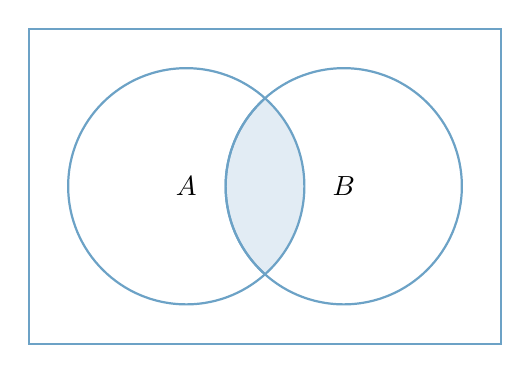
\begin{tikzpicture}
                    % Define the circles for sets A and B
                    \def\firstcircle{(0,0) circle (1.5cm)}
                    \def\secondcircle{(0:2cm) circle (1.5cm)}
                    
                    % Draw the rectangle to represent the universal set
                    \draw[outline] (-2,-2) rectangle (4,2);
                    
                    % Draw the circles A and B
                    \begin{scope}
                        \clip \firstcircle;
                        \fill[filled] \secondcircle;
                    \end{scope}
                    \draw[outline] \firstcircle node {$A$};
                    \draw[outline] \secondcircle node {$B$};
                \end{tikzpicture}
                \caption{$A \cap B$}
                \label{fig:venn1}
            \end{subfigure}
            \hfill
              \begin{subfigure}[b]{0.45\textwidth}
                        \centering
                        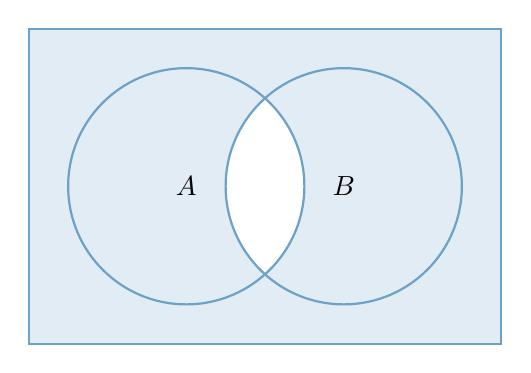
\begin{tikzpicture}
                            \def\firstcircle{(0,0) circle (1.5cm)}
                            \def\secondcircle{(0:2cm) circle (1.5cm)}
                            
                            % Draw the rectangle to represent the universal set
                            \fill[filled] (-2,-2) rectangle (4,2);
                            
                            % Draw the circles and fill the intersection with white
                            \begin{scope}
                                \clip \firstcircle;
                                \fill[white] \secondcircle;
                            \end{scope}
                            \draw[outline] \firstcircle node {$A$};
                            \draw[outline] \secondcircle node {$B$};
                        \end{tikzpicture}
                        \caption{$\skoverline{A \cap B}$}
                        \label{fig:venn2}
                    \end{subfigure}

            % Second row
            \vspace{10pt} % Adjust spacing between rows
            \begin{subfigure}[b]{0.45\textwidth}
                \centering
                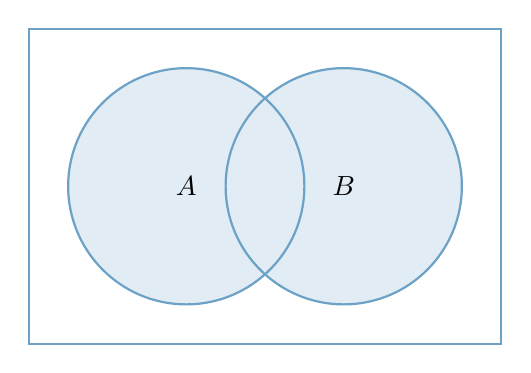
\begin{tikzpicture}
                    \def\firstcircle{(0,0) circle (1.5cm)}
                    \def\secondcircle{(0:2cm) circle (1.5cm)}
                    
                    % Draw the rectangle to represent the universal set
                    \draw[outline] (-2,-2) rectangle (4,2);
                    
                    \draw[filled] \firstcircle node {$A$}
                                  \secondcircle node {$B$};
                \end{tikzpicture}
                \caption{$A \cup B$}
                \label{fig:venn3}
            \end{subfigure}
            \hfill
            \begin{subfigure}[b]{0.45\textwidth}
                \centering
                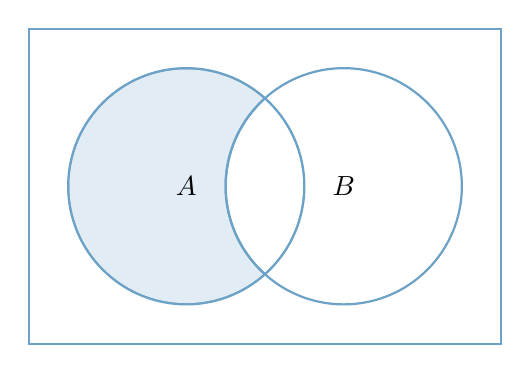
\begin{tikzpicture}
                    \def\firstcircle{(0,0) circle (1.5cm)}
                    \def\secondcircle{(0:2cm) circle (1.5cm)}
                    
                    % Draw the rectangle to represent the universal set
                    \draw[outline] (-2,-2) rectangle (4,2);
                    
                    \begin{scope}
                        \clip \firstcircle;
                        \draw[filled, even odd rule] \firstcircle node {$A$}
                                                     \secondcircle;
                    \end{scope}
                    \draw[outline] \firstcircle
                                   \secondcircle node {$B$};
                \end{tikzpicture}
                \caption{$A - B$}
                \label{fig:venn4}
            \end{subfigure}
        \end{figure}
        %\setlength{\parskip}{0mm} % Reset the value to avoid large spaces after the figure
\newpage

        \begin{figure}[h]
            \ContinuedFloat
            \centering
            % Third row
            %\vspace{10pt} % Adjust spacing between rows
            \begin{subfigure}[b]{0.45\textwidth}
                \centering
                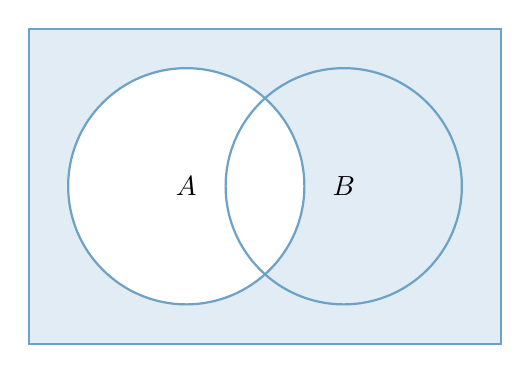
\begin{tikzpicture}
                    % Define the circles for sets A and B
                    \def\firstcircle{(0,0) circle (1.5cm)}
                    \def\secondcircle{(0:2cm) circle (1.5cm)}
                    
                    % Draw the rectangle to represent the universal set
                    \fill[filled] (-2,-2) rectangle (4,2);
                    
                    % Draw the circles and fill the part not in A with white
                    \begin{scope}
                        \clip \firstcircle;
                        \fill[white] (-2,-2) rectangle (4,2);
                    \end{scope}
                    \draw[outline] \firstcircle node {$A$};
                    \draw[outline] \secondcircle node {$B$};
                \end{tikzpicture}
                \caption{$\skoverline{A}$}
                \label{fig:venn5}
            \end{subfigure}
            \hfill
            \begin{subfigure}[b]{0.45\textwidth}
                \centering
                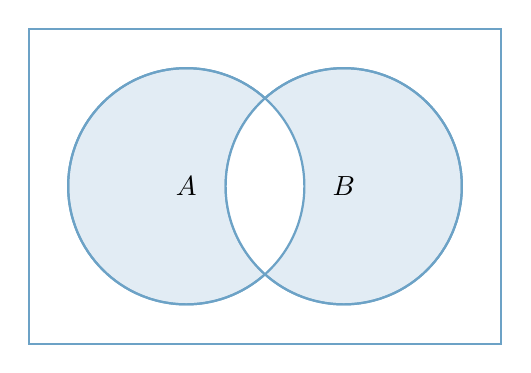
\begin{tikzpicture}
                    % Define the circles for sets A and B
                    \def\firstcircle{(0,0) circle (1.5cm)}
                    \def\secondcircle{(0:2cm) circle (1.5cm)}
                    
                    % Draw the rectangle to represent the universal set
                    \draw[outline] (-2,-2) rectangle (4,2);
                    
                    % Draw XOR by filling parts of A and B excluding their intersection
                    \fill[filled, even odd rule] \firstcircle node {};
                    \fill[filled, even odd rule] \secondcircle node {};
                    \begin{scope}
                        \clip \firstcircle;
                        \fill[white] \secondcircle;
                    \end{scope}
                    \begin{scope}
                        \clip \secondcircle;
                        \fill[white] \firstcircle;
                    \end{scope}
                    
                    % Outline the circles
                    \draw[outline] \firstcircle node {$A$};
                    \draw[outline] \secondcircle node {$B$};
                \end{tikzpicture}
                \caption{$A \triangle B$ (\texttt{XOR})}
                \label{fig:venn_xor}
            \end{subfigure}
            
            \vspace{10pt} % Adjust spacing between rows
            \begin{subfigure}[b]{0.5\textwidth}
                \centering
                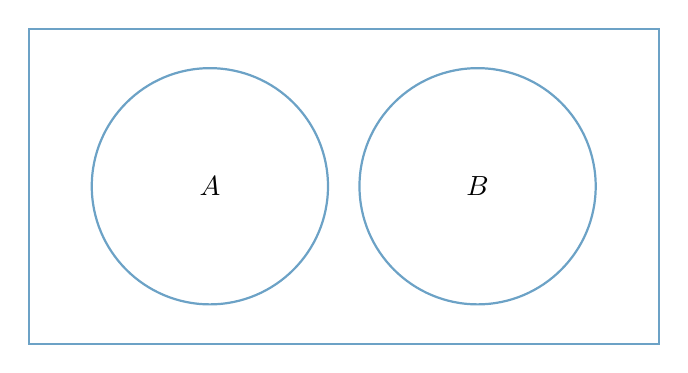
\begin{tikzpicture}
                    % Draw the rectangle to represent the universal set
                    \draw[outline] (-3,-2) rectangle (5,2);
                    
                    % Draw the circles for mutually exclusive events, moved closer
                    \draw[outline] (-0.7,0) circle (1.5cm) node {$A$};
                    \draw[outline] (2.7,0) circle (1.5cm) node {$B$};
                \end{tikzpicture}
                \caption{Mutually Exclusive (Disjoint)}
                \label{fig:venn6}
            \end{subfigure}
            \caption{Venn Diagrams Illustrating Various Set Operations}
            \label{fig:venn_diagrams}
        \end{figure}
        
        %\setlength{\parskip}{0mm} % Reset the value to avoid large spaces after the figure

\section{Counting Principles}

In many problems across mathematics, computer science, and engineering, determining the number of ways certain events can occur is important. Whether you're arranging elements, selecting groups, or navigating through complex scenarios, counting techniques provide the foundational tools to solve these problems. These techniques go beyond simple arithmetic and allow us to tackle questions like:

\begin{itemize}
    \item How many ways can we arrange a set of objects?
    \item In how many different paths can a process unfold?
    \item What is the probability of a specific event occurring given multiple possibilities?
\end{itemize}

Counting techniques, such as permutations, combinations, and the multiplication rule, help us quantify these possibilities systematically.

\subsection*{Multiplication Rule}

We start out by discussing the most basic counting principle: the \textbf{multiplication rule}:

\begin{theorem}[Multiplication Rule]
    Let an operation be described as a sequence of $k$ steps. Assume the following conditions:
    
    \begin{itemize}
        \item There are $n_1$ ways to complete step 1.
        \item There are $n_2$ ways to complete step 2 for each way of completing step 1.
        \item There are $n_3$ ways to complete step 3 for each way of completing step 2, and so on.
    \end{itemize}
    
    Then, the total number of ways to complete the entire operation is given by:
    
    \[
    n_1 \times n_2 \times \cdots \times n_k.
    \]
\end{theorem}
    
\begin{example}
    Suppose you are choosing a meal at a restaurant. You have the following options:
        
    \begin{itemize}
            \item 3 choices for the main course.
            \item 4 choices for the side dish.
            \item 2 choices for the drink.
    \end{itemize}
        
    Using the multiplication rule, the total number of ways to choose a meal is:
        
    \[
        3 \times 4 \times 2 = 24.
    \]
        
    Therefore, there are 24 different meal combinations available.
\end{example}

\begin{example} Automobile Options

An automobile manufacturer provides vehicles equipped with selected
options. Each vehicle is ordered

\begin{itemize}
    \item With or without an automatic transmission
    \item With or without a sunroof
    \item With one of three choices of a stereo system
    \item With one of four exterior colors
\end{itemize}

If the sample space consists of the set of all possible vehicle types, what is the number of outcomes in the sample space?
\end{example}

\begin{solution}
Using the multiplication rule, we can calculate the total number of possible vehicle types by multiplying the number of choices for each option:

\begin{itemize}
    \item 2 choices for the transmission (with or without automatic transmission)
    \item 2 choices for the sunroof (with or without sunroof)
    \item 3 choices for the stereo system
    \item 4 choices for the exterior color
\end{itemize}

Therefore, the total number of possible vehicle types is:

\[
2 \times 2 \times 3 \times 4 = 48
\]

So, there are 48 different possible vehicle types in the sample space.
\end{solution}

\subsection*{Replacement and Order in Counting}

Next we turn to an important distinction between with and without replacement in counting principles:

\begin{definition}[Counting with and without Replacement]
    When counting the number of ways to select objects from a set, two common scenarios are:

    \begin{itemize}
        \item \textbf{With Replacement}: An object can be selected more than once.
        \item \textbf{Without Replacement}: Once an object is selected, it cannot be chosen again.
    \end{itemize}
    \end{definition}
    
\begin{example}
    Suppose you have a bag containing 5 different colored balls. You draw 2 balls:
\begin{itemize}
    \item \textbf{With Replacement}: The first ball is placed back in the bag before drawing the second. There are \(5 \times 5 = 25\) possible outcomes.
    \item \textbf{Without Replacement}: The first ball is not placed back, so the number of outcomes is \(5 \times 4 = 20\).
\end{itemize}
\end{example}

\begin{example}
    Three people are drawing cards one after another from a standard deck of 52 cards. The goal is to find the Ace of Spades. Let's examine the two scenarios: with replacement and without replacement.

    \textbf{Without Replacement}

    In this scenario, each card drawn is not put back into the deck, reducing the total number of cards available after each draw.
    \begin{itemize}
        \item First Draw: The first person has a $\frac{1}{52}$ chance of drawing the Ace of Spades.
        \item Second Draw: If the first person does not draw the Ace of Spades, there are now 51 cards left, and the second person has a $\frac{1}{51}$ chance of drawing the Ace of Spades.
        \item Third Draw: If the Ace of Spades has not been drawn by the first two people, the third person has a $\frac{1}{50}$ chance of drawing it.
    \end{itemize}
    
    The probabilities change with each draw because the total number of cards decreases, and previously drawn cards are not available.
    
    \textbf{With Replacement}

    In this scenario, each card drawn is returned to the deck and reshuffled before the next person draws. This keeps the total number of cards constant.
    \begin{itemize}
        \item First Draw: The first person has a $\frac{1}{52}$ chance of drawing the Ace of Spades.
        \item Second Draw: Since the card is replaced and shuffled back into the deck, the second person also has a $\frac{1}{52}$ chance of drawing the Ace of Spades.
        \item Third Draw: Similarly, the third person has a $\frac{1}{52}$ chance of drawing the Ace of Spades.
    \end{itemize}
    
    The probabilities remain the same for each draw because the deck is reset to its original state after each draw.

\end{example}

\begin{example}
    Imagine you have a group of 5 students: Alice, Bob, Charlie, David, and Eve. You need to select 2 of them for different scenarios, illustrating when the order of selection matters and when it does not.
    \begin{itemize}
        \item \textbf{Order Matters}: Selecting Alice as Captain and Bob as Assistant Captain is a different outcome than selecting Bob as Captain and Alice as Assistant Captain.
        \end{itemize}
    Now, imagine you are simply selecting 2 students to form a study group with no specific roles assigned. Here, the order does not matter.
    \begin{itemize}
        \item \textbf{Order does not matters:}  Choosing Alice and Bob is considered the same outcome as choosing Bob and Alice; there is no distinction between the two orders since there are no assigned roles.
    \end{itemize}
    \label{ex:order_matters}
\end{example}

Example \ref{ex:order_matters} illustrates the distinction between \textit{permutations} and \textit{combinations}, two fundamental counting principles that are widely used in probability theory and combinatorics.

\begin{definition}[Permutation and Combination]
    \begin{itemize}
        \item \textbf{Permutation (Order Matters)}: Different sequences are counted as distinct outcomes, leading to a higher count.
        \item \textbf{Combination (Order Does Not Matter)}: Sequences are treated as identical, resulting in a lower count.
    \end{itemize}
\end{definition}

We will first discuss permutations, which are used when the order of selection matters.

\subsection*{Permutations}

Consider a set of elements, such as $S=\{a, b, c\}$. A permutation of the elements is an ordered sequence of the elements. For example, $a b c, a c b, b a c, b c a, c a b$, and $c b a$ are all of the permutations of the elements of $S$.

\begin{definition}[Permutations of \(n\) Objects]
    The permutation of \(n\) objects, i.e. an ordered arrangement of \(n\) objects, is \(n!\) (read as "n factorial"), where:
    \[
    n! = n \times (n-1) \times (n-2) \times \cdots \times 1
    \]
\end{definition}

This outcome is a direct application of the multiplication rule. To form a permutation, you start by choosing an element for the first position from the total of $n$ elements. Next, you choose an element for the second position from the remaining $n-1$ elements, then for the third position from the remaining $n-2$ elements, and continue this way until all positions are filled. Such arrangements are often called linear permutations.

\begin{example}
    It is said that any shuffling of a deck of card has only happened once in history. This is because the number of ways to shuffle a deck of 52 cards is \(52!\), which is an astronomically large number.

    \[52! \approx 8.07 \times 10^{67}\]
\end{example}

\begin{example}
    Suppose you have 5 different books on a shelf. You want to rearrange them in a different order. The number of ways to rearrange the books is
    \[5! = 5 \times 4 \times 3 \times 2 \times 1 = 120\]
\end{example}

There are cases where we are only interested in arranging a subset of elements from a larger set. The formula for counting these arrangements also derives from the multiplication rule.

\begin{definition}[Permutations of Subsets]
    The number of permutations of subsets of $r$ elements selected from a set of $n$ different elements is
    \[
    P_r^n=n \times(n-1) \times(n-2) \times \cdots \times(n-r+1)=\frac{n!}{(n-r)!}
    \]
\end{definition}

\begin{example}
    Suppose you have 5 different books on a shelf, and you want to rearrange 3 of them in a different order. The number of ways to rearrange the 3 books is
    \[
    P_3^5=5 \times 4 \times 3 = 60
    \]
\end{example}

\begin{example}
    There are 10 entries in a contest. Only three will win, $1^{\text {st }}, 2^{\text {nd }}$, or $3^{\text {rd }}$ prize. What are the possible results?
\end{example}
\begin{solution}
    The number of ways to award the prizes is the number of permutations of 3 objects selected from 10, which is
    \[
    P_3^{10}= \frac{10!}{(10-3)!}=\frac{10!}{7!} = 10 \times 9 \times 8 = 720
    \]
    Therefore, there are 720 possible outcomes for awarding the prizes.
\end{solution}

\subsection*{Combinations}

When the order of selection does not matter, we use the concept of combinations. Combinations are used when we are interested in selecting a subset of elements from a larger set without regard to the order in which they are selected. Let is start out with a couple of examples to illustrate the concept of combinations.

\begin{example}
    Suppose you have a group of 5 students: Alice, Bob, Charlie, David, and Eve. You need to select 2 of them to form a study group. The order in which you select the students does not matter. The possible combinations are:
    \begin{itemize}
        \item Alice and Bob
        \item Alice and Charlie
        \item Alice and David
        \item Alice and Eve
        \item Bob and Charlie
        \item Bob and David
        \item Bob and Eve
        \item Charlie and David
        \item Charlie and Eve
        \item David and Eve
    \end{itemize}
    The order of the students in the study group does not matter, so the combinations are considered identical.
\end{example}

\begin{example}
    Maria has three tickets for a concert. She'd like to use one of the tickets herself. She could then offer the other two tickets to any of four friends (Ann, Beth, Chris, Dave). How many ways can 2 people be selected from 4 to go to a concert?
\end{example}

\begin{example}
A circuit board has four different locations in which a component can be placed. If three identical components are to be placed on the board, how many different designs are possible?
\end{example}

\begin{solution}
    Since you can only place one component in each slot, placing a component in any slot immediately restricts the choices for the next component.
        
    \begin{enumerate}
        \item Fill slots 1, 2, and 3.
        \item Fill slots 1, 2, and 4.
        \item Fill slots 1, 3, and 4.
        \item Fill slots 2, 3, and 4.
    \end{enumerate}
\end{solution}

These examples illustrate the concept of combinations, where the order of selection does not matter. The formula for combinations is derived from the permutation formula by dividing out the number of ways to arrange the $r$ elements.

\begin{definition}[Combinations]
    The number of combinations of $r$ elements selected from a set of $n$ different elements is given by
    \[
    C_r^n = \binom{n}{r} = \frac{n!}{r!(n-r)!}
    \]
\end{definition}

This is also sometimes referred to as the \textbf{binomial coefficient}, denoted by $\binom{n}{r}$, which is read as "n choose r". It is called the binomial coefficient because it appears in the binomial theorem, which expands the powers of a binomial expression:

\begin{theorem}
    In algebra, the binomial coefficient is used to expand powers of binomials. According to the binomial theorem

$$
(a+b)^n=\sum_{k=0}^n\binom{n}{k} a^k b^{n-k}
$$

\end{theorem}

The theorem states that the expansion of the binomial expression $(a+b)^n$ is the sum of the terms $\binom{n}{k} a^k b^{n-k}$ for $k=0,1,2,\ldots,n$. The binomial coefficient $\binom{n}{k}$ gives the number of ways to choose $k$ elements from a set of $n$ elements. We will place no more emphasis on the binomial theorem here, but it is a fundamental concept in algebra and combinatorics, and is widely used in probability theory.

\section{Probability Basics}
In this section, we explore probability within discrete sample spaces — those with a finite or countably infinite set of outcomes.

Probability quantifies the likelihood or chance that an outcome of a random experiment will occur. For instance, when you hear, “The chance of rain today is 30\%,” it expresses our belief about the likelihood of rain. Probabilities are numbers assigned to outcomes, ranging from 0 to 1 (or equivalently, from 0\% to 100\%). A probability of 0 means the outcome will not happen, while a probability of 1 means it will happen for sure.

Probabilities can be interpreted in different ways:

\begin{itemize}
    \item \textbf{Objective (or Classical) Probability}: Often referred to as classical probability, this approach is used when outcomes are equally likely, such as in rolling a fair die or flipping a coin. Probabilities are assigned based on the assumption that each outcome has an equal chance of occurring. For example, when rolling a fair six-sided die, the probability of rolling a 3 is \( \frac{1}{6} \) because there are 6 equally likely outcomes (1, 2, 3, 4, 5, 6), and only one of them is a 3. The probability is the same for all observers.
        
    \item \textbf{Relative Frequency (Empirical Probability)}: Empirical probability is based on observations from experiments rather than theoretical calculations. For example, if a software tester runs a stress test on a server 100 times and it crashes 7 times, the empirical probability of a crash is \( \frac{7}{100} = 0.07 \). This approach relies on actual data rather than assumptions or intuition.
        
    \item \textbf{Subjective Probability}: This reflects our personal belief or degree of confidence in an outcome. Different people might assign different probabilities to the same event based on their knowledge or perspective. You and your friends discuss Denmark’s chances of winning the World Cup. Based on recent performance and team strength, you estimate a 10\% chance. However, a more optimistic friend assigns a 20\% chance, while another gives only 5\%, considering stronger competitors. This illustrates subjective probability, where each person's estimate varies based on personal beliefs and biases rather than objective data.
    

\end{itemize}

When assigning probabilities, it’s essential that the sum of all probabilities in an experiment equals 1, ensuring consistency with the relative frequency interpretation.

We start by establishing the Axioms of Probability, which lay the foundation for how probabilities are assigned to events. These axioms define the basic properties that every probability measure must satisfy.
    
\begin{axiom}[Axioms of Probability]
    \begin{itemize}
        \item \textbf{Axiom 1:} For any event \(A\), \( 0 \leq P(A) \leq 1 \).
        \item \textbf{Axiom 2:} Probability of the sample space \(S\) is \(P(S) = 1\).
        \item \textbf{Axiom 3:} If \(A_1, A_2, A_3, \cdots\) are disjoint events, then \(P\left(A_1 \cup A_2 \cup A_3 \cdots\right) = P\left(A_1\right) + P\left(A_2\right) + P\left(A_3\right) + \cdots\)
    \end{itemize}
\end{axiom}

The property that \( 0 \leq P(A) \leq 1 \) is equivalent to the requirement that a relative frequency must be between 0 and 1. The property that \( P(S) = 1 \) is a consequence of the fact that an outcome from the sample space occurs on every trial of an experiment. Consequently, the relative frequency of \( S \) is 1. Property 3 implies that if the events \( A_1 \) and \( A_2 \) have no outcomes in common, the relative frequency of outcomes in \( A_1 \cup A_2 \) is the sum of the relative frequencies of the outcomes in \( A_1 \) and \( A_2 \).

In the next sections we will see more about the probability of events and how to calculate them.

\subsection*{Probability of an Event}
The probability of an event is a measure of the likelihood that the event will occur. It is denoted by \( P(A) \), where \( A \) is the event. The probability of an event ranges from 0 to 1, where 0 indicates that the event will not occur, and 1 indicates that the event will occur for sure.

\begin{definition}[Probability of an Event]
    The probability of an event \( A \), denoted by \( P(A) \), is the likelihood that event \( A \) will occur. It is defined as the ratio of the number of favorable outcomes to the total number of outcomes in the sample space.
    \[
    P(A) = \frac{\text{Number of favorable outcomes}}{\text{Total number of outcomes}}
    \]
\end{definition}

\begin{example}
    Suppose you are testing a software module with 10 different test cases. Out of these, 3 test cases are known to fail due to a bug. If you randomly select one test case to run, what is the probability that the selected test case will fail?
\end{example}

\begin{solution}
    Here, the event $A$ is "the test case fails."
\begin{itemize}
    \item Number of favorable outcomes (failing test cases) $=3$
    \item Total number of outcomes (total test cases) $=10$
\end{itemize}

Using the formula:

$$
P(A)=\frac{\text { Number of favorable outcomes }}{\text { Total number of outcomes }}=\frac{3}{10}=0.3
$$


Therefore, the probability that a randomly selected test case will fail is 0.3 , indicating that there is a $30 \%$ chance of failure.

\end{solution}

\begin{example}
    Imagine a software development environment where you have 50 files, consisting of 20 Python scripts, 15 Java files, and 15 configuration files. If you randomly select one file to edit, what is the probability that the file is a Python script?
\end{example}

\begin{solution}
Here, the event $A$ is "the selected file is a Python script."
\begin{itemize}
    \item Number of favorable outcomes (Python scripts) $=20$
    \item Total number of outcomes (total files) $=50$
\end{itemize}

Using the formula:

$$
P(A)=\frac{\text { Number of favorable outcomes }}{\text { Total number of outcomes }}=\frac{20}{50}=0.4
$$

Thus, the probability of selecting a Python script is 0.4 , meaning there is a $40 \%$ chance of choosing a Python file from the set.

\end{solution}

\section{Probability of Joint Events and Set Operations}
Joint events are formed by applying basic set operations to individual events. Commonly, we encounter unions of events, such as $A \cup B$; intersections of events, such as $A \cap B$; and complements of events, such as $\skoverline{A}$. These combined events are often of particular interest, and their probabilities can frequently be derived from the probabilities of the individual events that compose them. Understanding these set operations is essential for accurately calculating the probability of joint events. In this section, we will explore how unions of events and other set operations can be used to determine the probabilities of more complex events.

When dealing with events, the intersection represents \texttt{AND} while the union represents \texttt{OR} The probability of the intersection of events $A$ and $B$, denoted as $P(A \cap B)$, can also be expressed as $P(A, B)$ or $P(A B)$:

\begin{custombox}{Notation}
    \begin{itemize}
        \item The probability of the intersection of events $A$ and $B$ is denoted as $P(A \cap B)$, $P(A, B)$, or $P(A B)$.
        \item The probability of the union of events $A$ and $B$ is denoted as $P(A \cup B)$.
        \item The probability of the complement of event $A$ is denoted as $P(\skoverline{A})$, $P(A^{\prime})$, or $P(A^c)$.
    \end{itemize}
\end{custombox}

From the axioms of probability, we can derive the following rules of probabilities:
\newpage
\begin{theorem}{Rules of Probability}
    \begin{itemize}
        \item \textbf{Complement Rule:} The probability of the complement of event $A$ is
    
        \[
        P(\skoverline{A}) = 1 - P(A)
        \]

        \item \textbf{Empty Set Rule:} The probability of the empty set is 0, i.e.,
        
        \[P(\emptyset) = 0\]
        
        \item \textbf{Addition Rule:} For any two events $A$ and $B$, the probability of the union of events $A$ and $B$ is given by
        \[
        P(A \cup B) = P(A) + P(B) - P(A \cap B)
        \]

        \item \textbf{Difference Rule:} The probability of the difference between events $A$ and $B$ is given by
        \[
        P(A-B)=P(A)-P(A \cap B)
        \]
        \item \textbf{Subset Rule:} If $A$ is a subset of $B$ ($A \subset B$), then
        \[P(A) \leq P(B)\].
    \end{itemize}
\end{theorem}

We can obtain the Complement Rule by noting:

\begin{align*}
    1 &= P(S) & \text{(axiom 2)} \\
      &= P(A \cup \skoverline{A}) & \text{(definition of complement)} \\
      &= P(A) + P(\skoverline{A}) & \text{(since } A \text{ and } \skoverline{A} \text{ are disjoint)}
\end{align*}

Since $\emptyset=\skoverline{S}$, we can apply part the Complement Rule to deduce that $P(\emptyset)=1-P(S)=0$. This is intuitive because, by definition, an event occurs when the outcome of the random experiment is part of that event. However, since the empty set contains no elements, no outcome of the experiment can ever belong to it, making its probability zero.

The Difference Rule can be obtained by showing that $P(A)=P(A \cap B)+P(A-B)$. Note that the two sets $A \cap B$ and $A-B$ are disjoint and their union is $A$. Thus, by the third axiom of probability

\begin{align*}
    P(A) &= P\left((A \cap B) \cup (A - B)\right) & \text{(since } A = (A \cap B) \cup (A - B)) \\
         &= P(A \cap B) + P(A - B) & \text{(since } A \cap B \text{ and } A - B \text{ are disjoint)}
    \end{align*}
    

The Addition Rule we obtain by noting that $A$ and $B-A$ are disjoint sets and their union is $A \cup B$. Thus,

\begin{align*}
    P(A \cup B) &= P(A \cup (B - A)) && (\text{since } A \cup B = A \cup (B - A)) \\
                &= P(A) + P(B - A) && (\text{since } A \text{ and } B - A \text{ are disjoint}) \\
                &= P(A) + P(B) - P(A \cap B) && (\text{by part the Difference Rule})
    \end{align*}
    
And finally the Subset Rule is a direct consequence of the fact that if $A \subset B$, then $B$ can be written as the union of $A$ and $B-A$. Since $A$ and $B-A$ are disjoint, we have $P(B)=P(A)+P(B-A) \geq P(A)$.

We conclude this section with a few examples illustrating the application of these rules to calculate probabilities of joint events.

\begin{example}
    A company has bid on two large construction projects. The company president believes that the probability of winning the first contract is 0.6, the probability of winning the second contract is 0.4, and the probability of winning both contracts is 0.2.

    \begin{enumerate}[label=(\alph*)]
        \item What is the probability that the company wins at least one contract?
        \item What is the probability that the company wins the first contract but not the second contract?
        \item What is the probability that the company wins neither contract?
        \item What is the probability that the company wins exactly one contract?
    \end{enumerate}
\end{example}

\begin{solution}
    Let $A$ be the event that the company wins the first contract, and $B$ be the event that the company wins the second contract. Given:
    \begin{itemize}
        \item $P(A) = 0.6$
        \item $P(B) = 0.4$
        \item $P(A \cap B) = 0.2$
    \end{itemize}
    
    \begin{enumerate}[label=(\alph*)]
        \item The probability that the company wins at least one contract is the probability of the union of events $A$ and $B$. Using the Addition Rule:
        
        \begin{align*}
            P(A \cup B) &= P(A) + P(B) - P(A \cap B) \\
                        &= 0.6 + 0.4 - 0.2 \\
                        &= 0.8
        \end{align*}
        
        Therefore, the probability that the company wins at least one contract is 0.8.
        
        \item The probability that the company wins the first contract but not the second contract is the probability of the difference between events $A$ and $B$. Using the Difference Rule:
        
        \begin{align*}
            P(A - B) &= P(A) - P(A \cap B) \\
                    &= 0.6 - 0.2 \\
                    &= 0.4
        \end{align*}
        
        Therefore, the probability that the company wins the first contract but not the second contract is 0.4.
        
        \item The probability that the company wins neither contract is the probability of the complement of the union of events $A$ and $B$. Using the Complement Rule:
        
        \begin{align*}
            P(\skoverline{A \cup B}) &= 1 - P(A \cup B) \\
                                    &= 1 - 0.8 \\
                                    &= 0.2
        \end{align*}
        
        Therefore, the probability that the company wins neither contract is 0.2.
        
        \item The probability that the company wins exactly one contract is the probability of the difference between the union of events $A$ and $B$ and the intersection of events $A$ and $B$. Using the Difference Rule:
            
            \begin{align*}
                P((A \cup B) - (A \cap B)) &= P(A \cup B) - P(A \cap B) \\
                                            &= 0.8 - 0.2 \\
                                            &= 0.6
            \end{align*}
            So, the probability that the company wins exactly one contract is 0.6.
            \end{enumerate}
\end{solution}

\newpage

\begin{example}
    \begin{itemize}
    \item There is a 60 percent chance that it will rain today.
    \item There is a 50 percent chance that it will rain tomorrow.
    \item There is a 30 percent chance that it does not rain either day.
    \end{itemize}
    
\begin{enumerate}[label=(\alph*)]
    \item The probability that it will rain today or tomorrow
    \item The probability that it will rain today and tomorrow.
    \item The probability that it will rain today but not tomorrow.
    \item The probability that it either will rain today or tomorrow, but not both.
\end{enumerate}
    
\begin{solution}
\begin{enumerate}[label=(\alph*)]
    \item     Let \( A \) be the event that it rains today, and \( B \) be the event that it rains tomorrow.
        
    Given:
    \begin{align*}
        P(A \cup B) &= 1 - P\left(\skoverline{(A \cup B)}\right) \quad &\text{by the Complement Rule} \\
                &= 1 - P\left(\skoverline{A} \cap \skoverline{B}\right) \quad &\text{by De Morgan's Law} \\
                &= 1 - 0.3 \\
                &= 0.7
    \end{align*}
            
        
    Therefore, the probability that it will rain today or tomorrow is \( 0.7 \).

    \item The probability that it will rain today and tomorrow: this is $P(A \cap B)$. To find this we note that
    \begin{align*}
    P(A \cap B) &= P(A) + P(B) - P(A \cup B) \\
                &= 0.6 + 0.5 - 0.7 \\
                &= 0.4
    \end{align*}

    \item The probability that it will rain today but not tomorrow: this is $P\left(A \cap \skoverline{B}\right)$.
    
    \begin{align*}
        P(A \cap \skoverline{B}) &= P(A - B) \\
                      &= P(A) - P(A \cap B) \\
                      &= 0.6 - 0.4 \\
                      &= 0.2
        \end{align*}
        
    \item The probability that it either will rain today or tomorrow but not both: this is $P(A-B)+P(B-A)$. We have already found $P(A-B)=.2$. Similarly, we can find $P(B-A)$:
    
    \begin{align*}
        P(B-A) & =P(B)-P(B \cap A) \\
        & =0.5-0.4 \\
        & =0.1
        \end{align*}
    Thus,
    \begin{align*}
        P(A-B)+P(B-A) &= 0.2+0.1 \\
                      &= 0.3
    \end{align*}
\end{enumerate}
\end{solution}
\end{example}

\chapter{An Introduction to Statistics}
\label{chap:ch6}

Statistics is the science of collecting, analyzing, interpreting, and presenting data. It provides the tools to move beyond raw information to genuine understanding. This field is broadly divided into two main branches:

\begin{enumerate}
    \item \textbf{Descriptive Statistics:} This focuses on summarizing and organizing data so that we can easily understand it. It's about describing what the data shows.
    \item \textbf{Inferential Statistics:} This involves using data from a small group (a sample) to make educated guesses or conclusions about a larger group (a population).
\end{enumerate}

In this chapter, we will focus on \textbf{Descriptive Statistics}. We will learn how to summarize data using measures of central tendency and dispersion, and how to visualize it using distributions and histograms. We will also see how the Python programming language, with its powerful libraries, makes performing these calculations and creating visualizations remarkably simple.

\section{Descriptive Statistics and Frequency Distributions}

The first step in any statistical analysis is to explore the data. Descriptive statistics gives us a set of tools to summarize the main features of a dataset. Instead of looking at a long list of numbers, we can describe its essential characteristics in just a few values or a simple chart.

\subsection{Frequency Distribution}
Imagine a teacher has just graded the final exam for a class of 20 students. The scores are:

82, 95, 71, 88, 79, 85, 92, 88, 76, 85, 88, 93, 74, 85, 82, 78, 88, 90, 85, 79

Looking at this raw list is not very helpful. A better way to organize this is with a \textbf{Frequency Distribution}, which shows how many times each score appears.

\begin{table}[htbp]
\centering
\caption{Frequency Distribution of Student Exam Scores.}
\begin{tabular}{|c|c|}
\hline
\textbf{Score} & \textbf{Frequency} \\
\hline
71 & 1 \\
74 & 1 \\
76 & 1 \\
78 & 1 \\
79 & 2 \\
82 & 2 \\
85 & 4 \\
88 & 4 \\
90 & 1 \\
92 & 1 \\
93 & 1 \\
95 & 1 \\
\hline
\end{tabular}
\end{table}

This table is much clearer. We can immediately see that the scores 85 and 88 are the most common.

\subsection{Histograms}
While a frequency table is useful, a visual representation is often even better. A \textbf{Histogram} is a bar chart that graphically displays a frequency distribution. Each bar represents a range of values (called a "bin"), and the height of the bar shows the frequency of data points that fall into that bin.

For the exam scores, we could group them into bins of 10 points (70-79, 80-89, etc.).

% \begin{figure}[htbp]
%     \centering
%     % NOTE: You need to have an image file named 'histogram_placeholder.png'
%     \includegraphics[width=0.7\textwidth]{histogram_placeholder.png}
%     \caption{A histogram of student exam scores, grouped into bins of 10 points.}
%     \label{fig:histogram}
% \end{figure}

The histogram instantly tells us a story: the vast majority of students scored in the 80s, with fewer in the 70s and 90s. This visual summary is a cornerstone of descriptive statistics.

\section{Measures of Central Tendency}

While a histogram gives us a general idea of the data's shape, we often want to summarize the data with a single number that represents the "center" or "typical" value. These are called \textbf{measures of central tendency}.

\subsection{Mean}
The \textbf{Mean} is the most common measure of central tendency. It is simply the sum of all the values in a dataset divided by the number of values. It's what most people refer to as the "average."

For a set of data $x_1, x_2, \ldots, x_n$, the formula for the sample mean ($\bar{x}$) is:
\[ \bar{x} = \frac{\sum_{i=1}^{n} x_i}{n} \]

For our exam scores, the sum is 1690. Since there are 20 students, the mean is:
\[ \bar{x} = \frac{1690}{20} = 84.5 \]
The mean score is 84.5. The mean is easy to calculate and uses all the data, but it can be heavily influenced by extremely high or low values, known as outliers.

\subsection{Median}
The \textbf{Median} is the middle value of a dataset that has been sorted in ascending order. It is the point that splits the data in half—50\% of the values are below it, and 50\% are above it.

To find the median of our 20 exam scores, we first sort them:
71, 74, 76, 78, 79, 79, 82, 82, 85, \textbf{85}, \textbf{85}, 85, 88, 88, 88, 88, 90, 92, 93, 95

Since we have an even number of values (20), the median is the average of the two middle values (the 10th and 11th).
\[ \text{Median} = \frac{85 + 85}{2} = 85 \]
The median score is 85. Unlike the mean, the median is not affected by outliers. If the top score was 100 instead of 95, or even 150, the median would still be 85.

\subsection{Mode}
The \textbf{Mode} is the value that appears most frequently in a dataset. A dataset can have one mode, more than one mode (bimodal or multimodal), or no mode at all.

Looking at our frequency table, we can see that two scores appear 4 times each: 85 and 88. Therefore, this dataset is \textbf{bimodal}, and the modes are 85 and 88. The mode is particularly useful for categorical data (e.g., "what is the most common car color?") but works for numerical data as well.

\section{Measures of Dispersion}

Measures of central tendency tell us where the center of the data is, but they don't tell us how spread out the data is. \textbf{Measures of Dispersion} (or variability) describe the spread. For example, two classes might both have a mean score of 80, but in one class, all scores are between 75 and 85, while in the other, scores range from 50 to 100.

\subsection{Variance}
The \textbf{Variance} measures how far each number in the set is from the mean. To calculate it, we take the difference between each value and the mean, square it, and then find the average of these squared differences. We square the differences to ensure they are all positive and to give more weight to larger deviations.

The formula for the sample variance ($s^2$) is:
\[ s^2 = \frac{\sum_{i=1}^{n} (x_i - \bar{x})^2}{n-1} \]
\textit{(Note: We divide by $n-1$ for a sample to get a better estimate of the population variance. This is known as Bessel's correction.)}

For our exam scores (with a mean of 84.5), the variance is approximately 48.9. The problem with variance is that its units are squared (e.g., "squared points"), which isn't very intuitive. This leads us to our next measure.

\subsection{Standard Deviation}
The \textbf{Standard Deviation} is simply the square root of the variance. This is an incredibly useful measure because it brings the unit of spread back to the original units of the data.

The formula for the sample standard deviation ($s$) is:
\[ s = \sqrt{s^2} = \sqrt{\frac{\sum_{i=1}^{n} (x_i - \bar{x})^2}{n-1}} \]

For our exam scores, the standard deviation is:
\[ s = \sqrt{48.9} \approx 6.99 \]
This tells us that, on average, a student's score is about 7 points away from the mean of 84.5. A small standard deviation means the data is tightly clustered around the mean, while a large standard deviation indicates the data is spread out.

\section{A Brief Introduction to the Normal Distribution}

If you create histograms for many different types of real-world data—such as people's heights, measurement errors, or blood pressure—you will often see a familiar shape emerge: a symmetric, bell-shaped curve. This is known as the \textbf{Normal Distribution} (or Gaussian distribution).

% \begin{figure}[htbp]
%     \centering
%     % NOTE: You need to have an image file named 'normal_dist_placeholder.png'
%     \includegraphics[width=0.6\textwidth]{normal_dist_placeholder.png}
%     \caption{A Normal Distribution curve, characterized by its bell shape.}
%     \label{fig:normal}
% \end{figure}

Key characteristics of the normal distribution:
\begin{itemize}
    \item It is \textbf{bell-shaped and symmetric}.
    \item The \textbf{mean, median, and mode are all equal} and are located at the center of the distribution.
    \item The spread of the curve is determined by the \textbf{standard deviation}.
\end{itemize}

The normal distribution is a cornerstone of inferential statistics and is used extensively in modeling. While we will explore it in much greater detail later, it is important to recognize it as a common and fundamental pattern in statistics.

\section{Using Python for Descriptive Statistics}

Manually calculating these statistics can be tedious, especially with large datasets. Fortunately, Python's scientific computing libraries make these tasks trivial. The primary libraries we use for this are \texttt{NumPy} for numerical calculations and \texttt{Matplotlib} for plotting.

Let's use Python to find all the statistics for our exam scores.

\begin{lstlisting}[language=Python, caption=Calculating descriptive statistics with Python., label=list:python-stats]
# First, we need to import the necessary libraries
import numpy as np
import matplotlib.pyplot as plt
from scipy import stats # SciPy has a good mode function

# Our exam scores data
scores = np.array([82, 95, 71, 88, 79, 85, 92, 88, 76, 85, 88, 93, 74, 85, 82, 78, 88, 90, 85, 79])

# --- Central Tendency ---
mean_score = np.mean(scores)
median_score = np.median(scores)
mode_score = stats.mode(scores)

print(f"Mean: {mean_score}")
print(f"Median: {median_score}")
print(f"Mode: {mode_score.mode} (appears {mode_score.count} times)")

# --- Dispersion ---
# Note: By default, NumPy calculates population variance/std.
# We use ddof=1 to calculate the sample variance/std.
variance_score = np.var(scores, ddof=1)
std_dev_score = np.std(scores, ddof=1)

print(f"Variance: {variance_score:.2f}")
print(f"Standard Deviation: {std_dev_score:.2f}")

# --- Visualization: Histogram ---
plt.hist(scores, bins=5, edgecolor='black') # Group scores into 5 bins
plt.title("Distribution of Exam Scores")
plt.xlabel("Score")
plt.ylabel("Frequency")
plt.show()
\end{lstlisting}

Running this code will output the values we calculated manually and generate a histogram, all in just a few lines of code. This demonstrates why Python is an essential tool for modern statistical analysis.


% \chapter{Linear Equations in Linear Algebra}\label{chap:ch7}

In 1949, Harvard Professor Wassily Leontief used one of the earliest computers, the Mark II, to solve a system of linear equations that modelled the U.S. economy. He divided the economy into 500 sectors, like coal, automotive, and communications, and described how each sector interacted using linear equations. Due to hardware limitations, he reduced the problem to 42 equations, which took the Mark II 56 hours to solve. This effort marked a milestone in computational applications, earning Leontief the 1973 Nobel Prize.

Leontief’s work showcased how linear algebra, combined with computing, could solve large-scale problems — an idea that resonates even more today in the realm of software engineering. Linear algebra is fundamental to many modern technologies, particularly in Machine Learning (ML) and Artificial Intelligence (AI). From powering recommendation systems to optimising neural networks, linear algebra is at the core of algorithms that drive today's intelligent systems.

In ML and AI, large datasets are transformed into matrices, where linear algebra techniques like matrix factorisation, eigenvalue decomposition, and singular value decomposition (SVD) are used to extract insights and make predictions. Neural networks, the backbone of AI, rely on linear algebra to propagate data through layers and adjust weights during training. As a software engineer, mastering these concepts in linear algebra equips you to build scalable, intelligent systems capable of tackling today’s most complex computational problems. 

With the exponential growth in data and computing, the significance of linear algebra in software development, especially in AI and ML, continues to rise. It is a vital tool that bridges theoretical mathematics with real-world applications in tech.

\section{Systems of Linear Equations}

Linear equations and their systems form the foundation of linear algebra, a critical area in mathematics with extensive applications in software engineering. From computer graphics to machine learning algorithms, understanding how to model and solve linear systems is essential for developing efficient and effective software solutions. We begin with a definition:

\begin{definition}{Linear Equations} A linear equation in the variables $x_1, x_2, \ldots, x_n$ is an equation that can be written in the form
\[
a_1 x_1 + a_2 x_2 + \cdots + a_n x_n = b
\]

where $b$ and the coefficients $a_1, \ldots, a_n$ are constants.

\end{definition}

Linear equations represent straight lines, planes, and hyperplanes in various dimensions, making them useful for modeling relationships in data and algorithms.

\begin{example} A line in two-dimensional space given by $y = m x + b$ is a linear equation. It can be rewritten to fit our standard form:

    \[
-m x+y=b
\]

Here, $a_1 = -m$, $a_2 = 1$, and $b$ is the constant term. \end{example}

\begin{example} The general equation of a plane in three-dimensional space is

\[
a x+b y+c z=d
\]

where $a$, $b$, $c$, and $d$ are constants. This equation is linear in the variables $x$, $y$, and $z$.
\end{example}

\begin{definition}{Systems of Linear Equations} A \textbf{system of linear equations} (also called a \textbf{linear system}) is a collection of one or more linear equations involving the same set of variables. \end{definition}

\begin{example} Consider the following system of linear equations in the variables $x_1, x_2, x_3$:
\[
\begin{aligned}
2x_1 + 3x_2 + x_3 &= 3 \\
7x_2 - 4x_3 &= 10 \\
x_3 &= 1
\end{aligned}
\]
This system contains three equations with three unknowns.

\end{example}

To solve the system, we first note from the third equation that $x_3 = 1$. Substituting this into the second equation, we solve for $x_2$:
\[
\begin{aligned}
7x_2 - 4(1) &= 10 \\
7x_2 &= 14 \\
x_2 &= 2
\end{aligned}
\]
Now, substituting $x_2 = 2$ and $x_3 = 1$ into the first equation, we solve for $x_1$:
\[
\begin{aligned}
2x_1 + 3(2) + 1 &= 3 \\
2x_1 &= -4 \\
x_1 &= -2
\end{aligned}
\]
Thus, the solution to the system is $\left(x_1, x_2, x_3\right) = (-2, 2, 1)$.

\begin{definition}{Solutions to a System of Linear Equations} A \textbf{solution} of a linear system in the variables $x_1, x_2, \ldots, x_n$ is a list of numbers $(s_1, s_2, \ldots, s_n)$ that satisfies all equations of the system when substituted for the variables $x_1, x_2, \ldots, x_n$, respectively. The set of all possible solutions is called its \textbf{solution set}. Two linear systems are called \textbf{equivalent} if they have the same solution set. \end{definition}

A system of linear equations has one of the following outcomes:
\begin{enumerate}[label=(\roman*)]
    \item \textbf{No solutions}, when the equations are inconsistent.
    \item \textbf{Exactly one solution}, when there is a unique set of values satisfying all equations.
    \item \textbf{Infinitely many solutions}, when there are multiple sets of values that satisfy the equations.
\end{enumerate}

We say a system is \textbf{consistent} if it has either one or infinitely many solutions. We say a system
is \textbf{inconsistent} if it has no solution. We formalise this later in this chapter.

\begin{remark} Determining whether a system is consistent addresses the \emph{existence} of solutions. If solutions exist, we may further explore the \emph{uniqueness} of these solutions. \end{remark}

\subsection*{Representing Systems with Matrices}
Matrices provide a compact and efficient way to represent and manipulate systems of linear equations, which is particularly beneficial in software applications involving large datasets.

\begin{definition} A \textbf{matrix} is a rectangular array of numbers arranged in rows and columns. The \textbf{coefficient matrix} of a linear system contains only the coefficients of the variables, while the \textbf{augmented matrix} includes an additional column for the constants from the right-hand side of the equations. \end{definition}

\begin{example} For the linear system:
\[
\begin{aligned}
2 x_1+3 x_2+x_3 & =3 \\
7 x_2-4 x_3 & =10 \\
x_3 & =1
\end{aligned}
\]

the coefficient matrix is:

\[
\left[\begin{array}{ccc}
2 & 3 & 1 \\
0 & 7 & -4 \\
0 & 0 & 1
\end{array}\right]
\]

and the augmented matrix is:

\[
\left[\begin{array}{ccc|c}
2 & 3 & 1 & 3 \\
0 & 7 & -4 & 10 \\
0 & 0 & 1 & 1
\end{array}\right]
\]

\end{example}

The vertical line between the coefficient part and the augmented part is optional and is used to visually separate the coefficients from the constants.

\begin{definition} The \textbf{size} of a matrix is defined by the number of its rows and columns, expressed as \emph{rows} $\times$ \emph{columns}. For instance, the coefficient matrix above is of size $3 \times 3$, and the augmented matrix is of size $3 \times 4$. \end{definition}

\subsection*{Solving Systems using Augmented Matrices}

We now illustrate how to solve a system of linear equations using augmented matrix notation. This process will be formalised in the next section but here we offer an example. This method streamlines the process of solving systems by focusing on matrix manipulations.

\begin{example}
    \label{ex:augmented-matrix}
Let $r_1$ denote the first row, $r_2$ the second row, and $r_3$ the third row.

\[
\left[\begin{array}{cccc}
2 & 3 & 1 & 3 \\
0 & 7 & -4 & 10 \\
0 & 0 & 1 & 1
\end{array}\right]
\]

To simplify the system, we perform \textit{elementary row operations}. Specifically, we adjust $r_1$ and $r_2$ as follows:
\[
\begin{aligned}
r_1 & \mapsto r_1 - r_3, \\
r_2 & \mapsto r_2 + 4r_3,
\end{aligned}
\]
which gives:
\[
\left[\begin{array}{cccc}
2 & 3 & 0 & 2 \\
0 & 7 & 0 & 14 \\
0 & 0 & 1 & 1
\end{array}\right]
\]

Next, we scale $r_2$ by $\frac{1}{7}$:
\[
r_2 \mapsto \frac{1}{7}r_2, \quad \left[\begin{array}{cccc}
2 & 3 & 0 & 2 \\
0 & 1 & 0 & 2 \\
0 & 0 & 1 & 1
\end{array}\right]
\]

Now, we eliminate the $3$ in the first row by performing:
\[
r_1 \mapsto r_1 - 3r_2, \quad \left[\begin{array}{cccc}
2 & 0 & 0 & -4 \\
0 & 1 & 0 & 2 \\
0 & 0 & 1 & 1
\end{array}\right]
\]

Finally, we scale $r_1$ by $\frac{1}{2}$ to get:
\[
r_1 \mapsto \frac{1}{2}r_1, \quad \left[\begin{array}{cccc}
1 & 0 & 0 & -2 \\
0 & 1 & 0 & 2 \\
0 & 0 & 1 & 1
\end{array}\right]
\]

We can now reinterpret the matrix as a linear system. From the augmented matrix, we find:
\[
\begin{aligned}
x_1 &= -2, \\
x_2 &= 2, \\
x_3 &= 1.
\end{aligned}
\]
This can be expressed compactly as:
\[
(x_1, x_2, x_3) = (-2, 2, 1).
\]
Thus, the solution is identical to the one we obtained through substitution.
\end{example}

\begin{example}
    \label{ex:inconsistent-system}
Determine if the following system is consistent:
        \[
            \begin{array}{r}
            x_2+4 x_3=2 \\
            x_1-3 x_2+2 x_3=6 \\
            x_1-2 x_2+6 x_3=9
            \end{array}
        \]
\end{example}

\begin{solution}
    First, we write the augmented matrix of the system:
    \[
    \left[\begin{array}{cccc}
    0 & 1 & 4 & 2 \\
    1 & -3 & 2 & 6 \\
    1 & -2 & 6 & 9
    \end{array}\right]
    \]
    
    To simplify the matrix, we interchange $r_1$ and $r_2$:
    \[
    r_1 \leftrightarrow r_2, \quad \left[\begin{array}{cccc}
    1 & -3 & 2 & 6 \\
    0 & 1 & 4 & 2 \\
    1 & -2 & 6 & 9
    \end{array}\right]
    \]
    
    Next, we eliminate the $1$ in the first column of $r_3$ by performing:
    \[
    r_3 \mapsto r_3 - r_1, \quad \left[\begin{array}{cccc}
    1 & -3 & 2 & 6 \\
    0 & 1 & 4 & 2 \\
    0 & 1 & 4 & 3
    \end{array}\right]
    \]
    
    Then, we eliminate the $1$ in the second column of $r_3$:
    \[
    r_3 \mapsto r_3 - r_2, \quad \left[\begin{array}{cccc}
    1 & -3 & 2 & 6 \\
    0 & 1 & 4 & 2 \\
    0 & 0 & 0 & 1
    \end{array}\right]
    \]
    
    The third row now corresponds to the equation:
    \[
    0x_1 + 0x_2 + 0x_3 = 1
    \]
    which simplifies to:
    \[
    0 = 1
    \]
    This is a contradiction, so the system is \textbf{inconsistent} and has no solution. \end{solution}

\begin{example}
    Give a solution of the following system (if one exists). Is it unique?
    \[
        \begin{aligned}
        x_1+2 x_2+3 x_3 & =4 \\
        3 x_1+6 x_2+9 x_3 & =12
        \end{aligned}
    \]
\end{example}

\begin{solution}
        \[
        \left[\begin{array}{cccc}
        1 & 2 & 3 & 4 \\
        3 & 6 & 9 & 12
        \end{array}\right]
        \]
        
        We observe that $r_2$ is a multiple of $r_1$:
        \[
        r_2 = 3r_1
        \]
        
        To simplify the system, we perform the following elementary row operation to eliminate redundancy:
        \[
        r_2 \mapsto r_2 - 3r_1,
        \]
        which yields:
        \[
        \left[\begin{array}{cccc}
        1 & 2 & 3 & 4 \\
        0 & 0 & 0 & 0
        \end{array}\right]
        \]
        
        The second row now consists entirely of zeros, indicating that it does not provide any new information. This means the system is underdetermined and has infinitely many solutions.
        
        We can express the first equation in terms of $x_1$:
        \[
        x_1 = 4 - 2x_2 - 3x_3
        \]
        
        Letting $x_2$ and $x_3$ be free variables (parameters), we set:
        \[
        x_2 = s, \quad x_3 = t, \quad \text{where } s, t \in \mathbb{R}
        \]
        
        Substituting back, we find:
        \[
        \begin{aligned}
        x_1 &= 4 - 2s - 3t, \\
        x_2 &= s, \\
        x_3 &= t.
        \end{aligned}
        \]
        
        This can be expressed compactly as:
        \[
        (x_1, x_2, x_3) = (4 - 2s - 3t, \ s, \ t), \quad \text{for all } s, t \in \mathbb{R}.
        \]
        
        The system has infinitely many solutions parameterized by $s$ and $t$. Therefore, the solution is not unique.\end{solution}

\begin{example}
    \label{ex:unique-solution}
    Choose $h$ and $k$ such that the following system
    \[
    \begin{aligned}
    x_1-3 x_2 & =1 \\
    2 x_1+h x_2 & =k
    \end{aligned}
    \]
    has
\begin{enumerate}[label=(\roman*)]
    \item a unique solution,
    \item many solutions, and
    \item no solution.
\end{enumerate}

\begin{solution}
        \[
        \left[\begin{array}{ccc}
        1 & -3 & 1 \\
        2 & h & k
        \end{array}\right]
        \]
        
        To simplify the system, we perform an elementary row operation to eliminate $x_1$ from the second equation. Specifically, we adjust $r_2$ as follows:
        \[
        r_2 \mapsto r_2 - 2r_1,
        \]
        which yields:
        \[
        \left[\begin{array}{ccc}
        1 & -3 & 1 \\
        0 & h + 6 & k - 2
        \end{array}\right]
        \]
        
        Now, we analyze the resulting system based on the value of $h + 6$.
        
        \textbf{Case 1: $h + 6 \ne 0$}
        
        When $h + 6 \ne 0$, we can solve for $x_2$ from the second equation:
        \[
        (h + 6)x_2 = k - 2 \implies x_2 = \dfrac{k - 2}{h + 6}
        \]
        Substituting $x_2$ back into the first equation:
        \[
        x_1 - 3x_2 = 1 \implies x_1 = 1 + 3x_2 = 1 + 3\left(\dfrac{k - 2}{h + 6}\right)
        \]
        Thus, we obtain a unique solution for $x_1$ and $x_2$. \textbf{The system has a unique solution when $h + 6 \ne 0$.}
        
        \newpage

        \textbf{Case 2: $h + 6 = 0$}
        
        When $h + 6 = 0$, i.e., $h = -6$, the second equation becomes:
        \[
        0x_2 = k - 2
        \]
        This simplifies to:
        \[
        0 = k - 2
        \]
        We have two subcases:
        
        \textbf{\textit{Subcase 2a:} $k - 2 = 0$}
        
          If $k = 2$, the equation becomes $0 = 0$, which is always true. The second equation provides no new information, so the system reduces to:
          \[
          x_1 - 3x_2 = 1
          \]
          Here, $x_2$ is a free variable. Solving for $x_1$:
          \[
          x_1 = 1 + 3x_2
          \]
          \textbf{The system has infinitely many solutions when $h = -6$ and $k = 2$.}
        
        \textbf{\textit{Subcase 2b:} $k - 2 \ne 0$}
        
          If $k \ne 2$, the equation becomes $0 = k - 2$, which is a contradiction since $0 \ne k - 2$. \textbf{Thus, the system has no solution when $h = -6$ and $k \ne 2$.}
                
        \textbf{Conclusion:}
        
        \begin{enumerate}[label=(\roman*)]
            \item \textbf{No solution} when $h = -6$ and $k \ne 2$.
            \item \textbf{A unique solution} when $h \ne -6$.
            \item \textbf{Infinitely many solutions} when $h = -6$ and $k = 2$.
        \end{enumerate} \end{solution}


\end{example}
\section{Elementary Row Operations and Echelon Forms}

In examples \ref{ex:augmented-matrix}-\ref{ex:unique-solution}, we performed a series of operations known as \textbf{elementary row operations}. These are fundamental transformations that simplify systems without changing their solution sets.

The three types of elementary row operations are:
\begin{itemize}
    \item \textbf{Replacement:} Replace one row by the sum of itself and a multiple of another row.
    \item \textbf{Interchange:} Swap two rows.
    \item \textbf{Scaling:} Multiply all entries in a row by a nonzero constant.
\end{itemize}

Two matrices are called \textbf{row equivalent} if one can be transformed into the other through a sequence of elementary row operations.

\begin{remark}
Two linear systems are equivalent (i.e., they have the same solution set) if their augmented matrices are row equivalent. Performing elementary row operations on an augmented matrix does not change the solution set of the system. \end{remark}

As you may have noticed in the examples, the matrices resulting from these operations often have a special pattern — lots of zeros below certain entries. This isn't just a coincidence but a goal in the process. We call this the \textbf{echelon form} of a matrix. By organizing a matrix into echelon form, we:

\begin{itemize}
    \item Make solving systems of linear equations easier.
    \item Systematically simplify the matrix, reducing the complexity of calculations.
    \item Reveal key properties about the system, like existence and number of solutions or whether certain equations are dependent.
\end{itemize}

\begin{definition}{Echelon Forms}
A matrix is in \textbf{echelon form} if it satisfies the following conditions:
\begin{enumerate}
    \item All zero rows are at the bottom.
    \item Each leading entry of a row is in a column to the right of the leading entry of the row above it.
    \item All entries in a column below a leading entry are zeros.
\end{enumerate}

In addition to echelon form, a matrix may also be in \textbf{reduced row echelon form} (RREF), which has the following properties:
\begin{enumerate}[resume]
    \item The leading entry in each nonzero row is 1.
    \item Each leading 1 is the only nonzero entry in its column.
\end{enumerate}
\end{definition}

We say that an echelon matrix $U$ is an echelon form of the matrix $A$ if $U$ is row equivalent to $A$. Similarly, we say that a reduced echelon matrix $U$ is the reduced echelon form of the matrix $A$ if $U$ is row equivalent to $A$.

The significance of putting the augmented matrix of a linear system in echelon form is explained by the
following theorem.

\begin{theorem}{Existence Theorem}
A linear system is consistent if and only if an echelon form of the augmented matrix has no row of the form
    \[
    \left[\begin{array}{llll}
    0 & \ldots & 0 & b
    \end{array}\right]
    \]
where $b$ is nonzero.
\end{theorem}

We saw an example of an inconsistent system in Example \ref{ex:inconsistent-system} because the echelon form of the augmented matrix has a row of the form $\left[\begin{array}{lll|l} 0 & 0 & 0 & 1 \end{array}\right]$. This row indicates that the system has no solution.

\begin{example}
    The augmented matrix of the linear system used as the main example in the preceding section,

\[
\left[\begin{array}{cccc}
2 & 3 & 1 & 3 \\
0 & 7 & -4 & 10 \\
0 & 0 & 1 & 1
\end{array}\right] , 
\] is already in echelon form. Since it has no row of the form mentioned in the theorem, we know immediately
that this system is consistent. The leading entries are $2$, $7$, and $1$, and all entries below them are zeros. This matrix is not in reduced row echelon form however because the leading entries are not all $1$.
\end{example}

Recall that we performed a sequence of row operations on the preceding matrix to get

\[
\left[\begin{array}{cccc}
1 & 0 & 0 & -2 \\
0 & 1 & 0 & 2 \\
0 & 0 & 1 & 1
\end{array}\right]
\]

which is in reduced echelon form. This allowed us easily to see the solutions of this system, which is the main advantage of putting the matrix in this form. This brings us to the following important theorem.

\begin{theorem}{Uniqueness of Reduced Echelon Form}
    Each matrix is row equivalent to one and only one reduced echelon matrix
\end{theorem}

A pivot position in a matrix $A$ is a location in $A$ that corresponds to a leading 1 in the reduced echelon form of $A$. A pivot column is a column of $A$ that contains a pivot position. Notice that you can obtain a pivot by scaling the leading entry of a row to be $1$. Therefore, the pivot column is the column of the leading entry.

We are now ready to present the algorithm for solving a system of linear equations using matrices.

\begin{custombox}{The Row Reduction Algorithm}
    Here we describe an algorithm for turning any matrix into an equivalent
    (reduced) echelon matrix. This algorithm is the foundation of solving systems of linear equations using matrices.

    \begin{enumerate}
        \item Begin with the leftmost nonzero column. This is a pivot column, with the pivot position at the top.
        \item Select a nonzero entry in the pivot column as a pivot. If necessary, interchange rows to move this entry into the pivot position.
        \item Use row replacement operations to create zeros in all positions below the pivot.
        \item Apply steps 1-3 to the submatrix of all entries below and to the right of the pivot position. Repeat this process until there are no more nonzero rows to modify. (At this point we have reached an echelon form of the matrix.)
        \item Beginning with the rightmost pivot and working upward and to the left, create zeros above each pivot using row operations. If a pivot is not 1, make it 1 by a scaling operation. (This step produces the reduced echelon form of the matrix.)
    \end{enumerate}

\end{custombox}

\subsection*{Solutions of Linear Systems}

Let $A$ be the coefficient matrix of a linear system. The pivot columns in the matrix correspond to what we call \textbf{basic variables}. The nonpivot columns correspond to what we call \textbf{free variables}.

\begin{example} Suppose the augmented matrix of a linear system has been reduced to the following form:

\[
\left[\begin{array}{lllll}
\blacksquare & * & * & * & * \\
0 & \blacksquare & * & * & * \\
0 & 0 & 0 & \blacksquare & * \\
0 & 0 & 0 & 0 & 0
\end{array}\right]
\]

where $\blacksquare$ represents any nonzero number, and $*$ represents any number (including 0 ). The basic variables of this system are $x_1, x_2$, and $x_4$. The only free variable is $x_3$.

\end{example}


\begin{theorem}{Uniqueness Theorem}
    If a linear system is consistent, then the solution set contains either
    \begin{enumerate}[label=(\roman*)]
        \item a unique solution, when there are no free variables, or
        \item infinitely many solutions, when there is at least one free variable.
    \end{enumerate}
\end{theorem}

\begin{example} Suppose the following matrix is the augmented matrix of a linear system in the variables $x_1, x_2$, and $x_3$. Row reduce the matrix to echelon form to determine if it is consistent.

\[
\left[\begin{array}{cccc}
1 & 2 & 3 & 4 \\
5 & 6 & 7 & 8 \\
9 & 10 & 11 & 12
\end{array}\right]
\]
If it is consistent, find the reduced echelon form and write the solution set using free variables as parameters.
\end{example}

\begin{solution} To simplify the system, we perform \textit{elementary row operations}.
        
    \textbf{Step 1: Eliminate the \( 5 \) in \( r_2 \)}
        
        We adjust \( r_2 \) as follows:
        \[
        r_2 \mapsto r_2 - 5r_1,
        \]
        which gives:
        \[
        \left[\begin{array}{cccc}
        1 & 2 & 3 & 4 \\
        0 & -4 & -8 & -12 \\
        9 & 10 & 11 & 12
        \end{array}\right]
        \]
        
    \textbf{Step 2: Eliminate the \( 9 \) in \( r_3 \)}
        
        We adjust \( r_3 \) as follows:
        \[
        r_3 \mapsto r_3 - 9r_1,
        \]
        which gives:
        \[
        \left[\begin{array}{ccc|c}
        1 & 2 & 3 & 4 \\
        0 & -4 & -8 & -12 \\
        0 & -8 & -16 & -24
        \end{array}\right]
        \]
        
    \textbf{Step 3: Eliminate the \( -8 \) in \( r_3 \)}
        
        We adjust \( r_3 \) again to eliminate the entry in the second column:
        \[
        r_3 \mapsto r_3 - 2r_2,
        \]
        which gives:
        \[
        \left[\begin{array}{cccc}
        1 & 2 & 3 & 4 \\
        0 & -4 & -8 & -12 \\
        0 & 0 & 0 & 0
        \end{array}\right]
        \]
        
    \newpage

    \textbf{Step 4: Scale \( r_2 \) to obtain a leading 1}
        
        We scale \( r_2 \) by \( -\dfrac{1}{4} \):
        \[
        r_2 \mapsto -\dfrac{1}{4} r_2,
        \]
        which gives:
        \[
        \left[\begin{array}{ccc|c}
        1 & 2 & 3 & 4 \\
        0 & 1 & 2 & 3 \\
        0 & 0 & 0 & 0
        \end{array}\right]
        \]
        
    \textbf{Step 5: Eliminate the \( 2 \) in \( r_1 \)}
        
        We adjust \( r_1 \) as follows:
        \[
        r_1 \mapsto r_1 - 2r_2,
        \]
        which gives:
        \[
        \left[\begin{array}{ccc|c}
        1 & 0 & -1 & -2 \\
        0 & 1 & 2 & 3 \\
        0 & 0 & 0 & 0
        \end{array}\right]
        \]
        
    At this point, the matrix is in \textit{reduced row-echelon form}.
        
    \textbf{Step 6: Interpret the matrix as a linear system}
        
        From the augmented matrix, we have:
        \[
        \begin{aligned}
        r_1 &: \quad x_1 - x_3 = -2, \\
        r_2 &: \quad x_2 + 2x_3 = 3, \\
        r_3 &: \quad 0 = 0.
        \end{aligned}
        \]
        
    Since the third row corresponds to the equation \( 0 = 0 \), which is always true, the system is \textbf{consistent}.
        
    \textbf{Step 7: Express the solution using a free variable}
        \[
        \begin{aligned}
        x_1 &= -2 + x_3, \\
        x_2 &= 3 - 2x_3, \\
        x_3 &= x_3.
        \end{aligned}
        \]      
\end{solution}

% \chapter{Vectors and Matrices}\label{chap:ch8}
A \textbf{vector} is a mathematical object that has both \textbf{magnitude} (length) and \textbf{direction}. In two or three dimensions, a vector is often represented as an arrow pointing from one point to another. For example, the vector \(\vect{v} = (x_1, x_2)\) in 2D space describes a movement from the origin \((0,0)\) to the point \((x_1, x_2)\).

Vectors are used to represent quantities like velocity, force, and displacement, which require both magnitude and direction to fully describe them. Vectors can be added together, scaled by a number, and decomposed into components.

Matrices, on the other hand, are rectangular arrays of numbers arranged in rows and columns. They are used to represent and solve systems of linear equations, perform transformations, and encode relationships between sets of vectors.

\section{Vectors in \texorpdfstring{$\mathbb{R}^2$}{R2} and \texorpdfstring{$\mathbb{R}^n$}{Rn}}

In linear algebra, vectors are often represented as \textbf{column matrices}. For example, the vector \(\vect{v} = (x_1, x_2)\) can be written as a column matrix:

\[ \vect{v} = \begin{bmatrix} x_1 \\ x_2 \end{bmatrix} \]

We say that two vectors are \textbf{equal} if and only if their corresponding entries are equal.

\begin{example}
    The following are vectors in $\mathbb{R}^2$ (a.k.a. the plane consisting of ordered pairs of real numbers):

    \[
    \vect{u}=\left[\begin{array}{l}
    3 \\
    5
    \end{array}\right], \quad \vect{v}=\left[\begin{array}{l}
    5 \\
    3
    \end{array}\right]
    \]
    They are not equal because their corresponding entries do not match.
\end{example}

\begin{figure}[htbp]
    \centering
    % First graph (points)
    \begin{minipage}{0.45\textwidth}
        \centering
        \begin{tikzpicture}
            % Draw the axes
            \draw[->] (-3, 0) -- (3, 0) node[right] {$x_1$};
            \draw[->] (0, -3) -- (0, 3) node[above] {$x_2$};

            % Plot the points
            \filldraw[headercolor] (-2,-1) circle (2pt) node[anchor=north east] {(-2, -1)};
            \filldraw[headercolor] (1,1) circle (2pt) node[anchor=south west] {(1, 1)};
            \filldraw[headercolor] (2,-2) circle (2pt) node[anchor=north west] {(2, -2)};
        \end{tikzpicture}
        \subcaption{Points in the plane}
    \end{minipage}
    \hfill
    % Second graph (vectors)
    \begin{minipage}{0.45\textwidth}
        \centering
        \begin{tikzpicture}
            % Draw the axes
            \draw[->] (-3, 0) -- (3, 0) node[right] {$x_1$};
            \draw[->] (0, -3) -- (0, 3) node[above] {$x_2$};

            % Plot the vectors
            \draw[->, thick, headercolor] (0,0) -- (-2,-1) node[anchor=north east] {(-2, -1)};
            \draw[->, thick, headercolor] (0,0) -- (1,1) node[anchor=south west] {(1, 1)};
            \draw[->, thick, headercolor] (0,0) -- (2,-2) node[anchor=north west] {(2, -2)};
        \end{tikzpicture}
        \subcaption{Vectors from the origin}
    \end{minipage}
    \caption{Points and vectors in the plane}
    \label{fig:points-vectors}
\end{figure}

The sum of two vectors $\vect{u}$ and $\vect{v}$ in $\mathbb{R}^2$, denoted $\vect{u} + \vect{v}$, is obtained by adding the corresponding entries of $\vect{u}$ and $\vect{v}$. Given a real number $c$, the scalar multiple of $\vect{u}$ by $c$, denoted $c \vect{u}$, is obtained by multiplying each entry in $\vect{u}$ by $c$.

\begin{example}
    If $\vect{u}$ and $\vect{v}$ are as in the preceding example, then 

$$
\begin{aligned}
\vect{u} + \vect{v} & =\left[\begin{array}{l}
3 \\
5
\end{array}\right] + \left[\begin{array}{l}
5 \\
3
\end{array}\right] = \left[\begin{array}{l}
3+5 \\
5+3
\end{array}\right] = \left[\begin{array}{l}
8 \\
8
\end{array}\right], \text { and } \\
6 \vect{u} & = 6\left[\begin{array}{l}
3 \\
5
\end{array}\right] = \left[\begin{array}{l}
6 \cdot 3 \\
6 \cdot 5
\end{array}\right] = \left[\begin{array}{l}
18 \\
30
\end{array}\right]
\end{aligned}
$$

\end{example}

\begin{remark}
    It is often helpful to identify a vector $\left[\begin{array}{l}a \\ b\end{array}\right] \in \mathbb{R}^2$ with a geometric point $(a, b)$ in the plane in order to get a picture of what we are working with.Please see figure \ref{fig:points-vectors} for an example.
\end{remark}

If $\vect{u}$ and $\vect{v}$ in $\mathbb{R}^2$ are thought of as points in the plane, then $\vect{u} + \vect{v}$ corresponds to the fourth vertex of the parallelogram whose other vertices are $\vect{0}, \vect{u}$, and $\vect{v}$.
Note: By $\vect{0}$, we mean the zero vector, or the vector whose entries are all zero. In $\mathbb{R}^2$, we have $\vect{0} = \left[\begin{array}{l}
0 \\
0
\end{array}\right]$.

We call this the \textit{parallelogram law of addition }and it can be seen in figure \ref{fig:parallelogram-law}.

\begin{figure}[htbp]
    \centering
    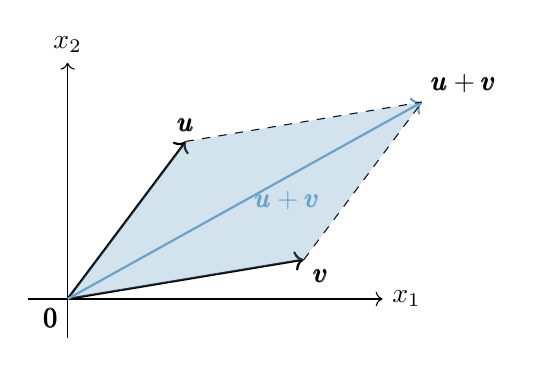
\begin{tikzpicture}
        \label{fig:parallelogram-law}

        % Draw axes
        \draw[->] (-0.5, 0) -- (4, 0) node[right] {$x_1$};
        \draw[->] (0, -0.5) -- (0, 3) node[above] {$x_2$};

        % Define the vectors u and v
        \coordinate (O) at (0, 0);
        \coordinate (U) at (1.5, 2);
        \coordinate (V) at (3, 0.5);
        \coordinate (UplusV) at (3+1.5, 2+0.5);

        % Draw vectors
        \draw[->, thick] (O) -- (U);
        \draw[->, thick] (O) -- (V);
        \draw[->, thick, headercolor] (O) -- (UplusV) node[midway, right] {$\vect{u} + \vect{v}$};

        % Draw the parallelogram
        \draw[dashed] (U) -- (UplusV);
        \draw[dashed] (V) -- (UplusV);
        \fill[headercolor, opacity=0.3] (O) -- (U) -- (UplusV) -- (V) -- cycle;

        % Add labels
        \node[above right] at (UplusV) {$\vect{u} + \vect{v}$};
        \node[above] at (U) {$\vect{u}$};
        \node[below right] at (V) {$\vect{v}$};

        % Mark the origin
        \node[below left] at (O) {$\vect{0}$};
    \end{tikzpicture}
    \caption{The parallelogram law of vector addition in $\mathbb{R}^2$.}
    \label{fig:parallelogram-law}
\end{figure}

These ideas generalise to higher-dimensional spaces. More specifically, we can define $\mathbb{R}^n$ as follows.

\begin{definition}
    For each positive integer $n$, we let $\mathbb{R}^n$ denote the collection of ordered $n$-tuples with each entry in $\mathbb{R}$. We often write these elements as $n \times 1$ matrices. We define addition and scalar multiplication of vectors in $\mathbb{R}^n$ in the same way as we do for $\mathbb{R}^2$. That is, we go coordinate-by-coordinate.
\end{definition}

\begin{example}
    If $u_1, u_2, \ldots, u_n \in \mathbb{R}$, then

    \[
    \vect{u} = \left[\begin{array}{c}
    u_1 \\
    u_2 \\
    \vdots \\
    u_n
    \end{array}\right] \in \mathbb{R}^n.
    \]
     
\end{example}

\begin{example}
    If $\vect{u}$ and $\vect{v}$ are in $\mathbb{R}^n$ (with entries denoted $u_1, \ldots, u_n$ and $v_1, \ldots, v_n$, respectively), and $c \in \mathbb{R}$, then

    \[
    \begin{aligned}
    & \vect{u} + \vect{v} = {\left[\begin{array}{c}
    u_1 \\
    u_2 \\
    \vdots \\
    u_n
    \end{array}\right] + \left[\begin{array}{c}
    v_1 \\
    v_2 \\
    \vdots \\
    v_n
    \end{array}\right] = \left[\begin{array}{c}
    u_1 + v_1 \\
    u_2 + v_2 \\
    \vdots \\
    u_n + v_n
    \end{array}\right], \text { and } } 
    & c \vect{u} = c\left[\begin{array}{c}
    u_1 \\
    u_2 \\
    \vdots \\
    u_n
    \end{array}\right] = \left[\begin{array}{c}
    c u_1 \\
    c u_2 \\
    \vdots \\
    c u_n
    \end{array}\right]
    \end{aligned}
    \]   
\end{example}

\begin{custombox}{Algebraic Properties of $\mathbb{R}^n$}
    Let $\vect{u}, \vect{v}, \vect{w} \in \mathbb{R}^n$ and $c, d \in \mathbb{R}$. Then the following properties hold:
    \begin{enumerate}
        \item \textbf{Commutative Property of Addition:} $\vect{u} + \vect{v} = \vect{v} + \vect{u}$.
        \item \textbf{Associative Property of Addition:} $(\vect{u} + \vect{v}) + \vect{w} = \vect{u} + (\vect{v} + \vect{w})$.
        \item \textbf{Additive Identity:} There exists a vector $\vect{0} \in \mathbb{R}^n$ such that $\vect{u} + \vect{0} = \vect{u}$ for all $\vect{u} \in \mathbb{R}^n$.
        \item \textbf{Additive Inverse:} For each $\vect{u} \in \mathbb{R}^n$, there exists a vector $-\vect{u} \in \mathbb{R}^n$ such that $\vect{u} + (-\vect{u}) = \vect{0}$.
        \item \textbf{Distributive Property:} $c(\vect{u} + \vect{v}) = c\vect{u} + c\vect{v}$ and $(c + d)\vect{u} = c\vect{u} + d\vect{u}$.
        \item \textbf{Associative Property of Scalar Multiplication:} $c(d\vect{u}) = (cd)\vect{u}$.
        \item \textbf{Multiplicative Identity:} $1\vect{u} = \vect{u}$.
    \end{enumerate}  
\end{custombox}

A \textbf{linear combination} is a way to combine vectors using scalar multiplication and addition. Given a set of vectors, we multiply each by a scalar and then sum the results. Linear combinations help us understand how vectors relate to each other and whether one vector can be expressed in terms of others.

\begin{definition}{Linear Combinations}
    Given a set of vectors $\vect{v}_1, \vect{v}_2, \ldots, \vect{v}_p \in \mathbb{R}^n$ and scalars $c_1, c_2, \ldots, c_p \in \mathbb{R}$, the vector $\vect{y}$ given by

\[
\vect{y} = c_1 \vect{v}_1 + \cdots + c_p \vect{v}_p
\]

is called a linear combination of $\vect{v}_1, \vect{v}_2, \ldots, \vect{v}_p$ with weights $c_1, c_2, \ldots, c_p$.

\end{definition}

\begin{example}
    Let $\vect{v}_1 = \left[\begin{array}{l}
        1 \\
        2
        \end{array}\right]$ and $\vect{v}_2 = \left[\begin{array}{c}
        1 \\
        -1
        \end{array}\right]$. Some linear combinations of $\vect{v}_1$ and $\vect{v}_2$ include
        
        \[
        \begin{aligned}
        \vect{0} & = 0 \vect{v}_1 + 0 \vect{v}_2 \\
        {\left[\begin{array}{l}
        3 \\
        0
        \end{array}\right] } & = \vect{v}_1 + 2 \vect{v}_2 \\
        {\left[\begin{array}{l}
        -5 \\
        -1
        \end{array}\right] } & = -2 \vect{v}_1 - 3 \vect{v}_2, \text { and } \\
        {\left[\begin{array}{l}
        5 \\
        1
        \end{array}\right] } & = 2 \vect{v}_1 + 3 \vect{v}_2
        \end{aligned}
        \]
        
\end{example}

\subsection*{Vector Equations and Linear Systems}

It is often the case that we wish to know if some vector $\vect{b}$ can be formed as a linear combination of some other set of vectors $\vect{a}_1, \ldots, \vect{a}_n$. The process for figuring this out is given by the following.

\begin{custombox}{Using Matrices to Determine Linear Combinations}
A vector equation

\[
x_1 \vect{a}_1 + x_2 \vect{a}_2 + \cdots + x_n \vect{a}_n = \vect{b}
\]

has the same solution set as the linear system whose augmented matrix is

\[
\left[\begin{array}{lllll}
\vect{a}_1 & \vect{a}_2 & \ldots & \vect{a}_n & \vect{b}
\end{array}\right].
\]    
\end{custombox}

More specifically, if the $\vect{a}_i$'s are in $\mathbb{R}^m$ with

\[
\vect{a}_1 = \left[\begin{array}{c}
a_{11} \\
a_{21} \\
\vdots \\
a_{m1}
\end{array}\right], \quad \vect{a}_2 = \left[\begin{array}{c}
a_{12} \\
a_{22} \\
\vdots \\
a_{m2}
\end{array}\right], \ldots, \quad \vect{a}_n = \left[\begin{array}{c}
a_{1n} \\
a_{2n} \\
\vdots \\
a_{mn}
\end{array}\right], \quad \text{and} \quad \vect{b} = \left[\begin{array}{c}
b_1 \\
b_2 \\
\vdots \\
b_m
\end{array}\right]
\]

then you would row reduce the matrix

\[
\begin{aligned}
& \left[\begin{array}{ccccc}
a_{11} & a_{12} & \ldots & a_{1n} & b_1 \\
a_{21} & a_{22} & \ldots & a_{2n} & b_2 \\
\vdots & \vdots & \ddots & \vdots & \vdots \\
a_{m1} & a_{m2} & \ldots & a_{mn} & b_m
\end{array}\right] \\
& \begin{array}{ccccc}
\hspace{0.5cm} \uparrow & \hspace{0.3cm} \uparrow & \hspace{0.0cm} \ldots & \hspace{0.2cm} \uparrow & \hspace{0.2cm} \uparrow \\
\hspace{0.4cm} \vect{a}_1 & \hspace{0.3cm} \vect{a}_2 & \hspace{0.1cm} \ldots & \hspace{0.2cm} \vect{a}_n & \hspace{0.2cm} \vect{b}
\end{array}
\end{aligned}
\]

to determine if there is some set of weights $x_1, \ldots, x_n$ that work.

\begin{example} Let
\[
\begin{aligned}
&\vect{a}_1=\left[\begin{array}{c}
2 \\
-1 \\
1
\end{array}\right], \quad \vect{a}_2=\left[\begin{array}{c}
0 \\
8 \\
-2
\end{array}\right], \quad \vect{a}_3=\left[\begin{array}{l}
6 \\
5 \\
1
\end{array}\right], \quad \text { and } \vect{b}=\left[\begin{array}{c}
10 \\
3 \\
7
\end{array}\right]
\end{aligned}
\]

We determine if $\vect{b}$ is a linear combination of $\vect{a}_1, \vect{a}_2, \vect{a}_3$, i.e. if there is some set of weights $x_1, x_2, x_3$ such that $x_1 \vect{a}_1 + x_2 \vect{a}_2 + x_3 \vect{a}_3 = \vect{b}$. By the above, we translate this question to the matrix setting.

\[
\begin{alignedat}{3}
& \left[\begin{array}{cccc}
2 & 0 & 6 & 10 \\
-1 & 8 & 5 & 3 \\
1 & -2 & 1 & 7
\end{array}\right]
& \quad & r_1 \leftrightarrow r_3 
& \quad & 
\left[\begin{array}{cccc}
1 & -2 & 1 & 7 \\
-1 & 8 & 5 & 3 \\
2 & 0 & 6 & 10
\end{array}\right] \\[10pt]
& & \quad & \begin{aligned}
    r_2 & \mapsto r_2 + r_1 \\
    r_3 & \mapsto r_3 - 2r_1
\end{aligned}
& \quad & 
\left[\begin{array}{cccc}
1 & -2 & 1 & 7 \\
0 & 6 & 6 & 10 \\
0 & 4 & 4 & -4
\end{array}\right] \\[10pt]
& & \quad & r_3 \mapsto r_3 - \frac{4}{6} r_2
& \quad & 
\left[\begin{array}{cccc}
1 & -2 & 1 & 7 \\
0 & 6 & 6 & 10 \\
0 & 0 & 0 & \blacksquare
\end{array}\right] .
\end{alignedat}
\]

Since the symbol $\blacksquare$ denotes something nonzero, we see that there's no solution, i.e. that $\vect{b}$ is not a linear combination of $\vect{a}_1, \vect{a}_2, \vect{a}_3$.

\end{example}

\begin{example} Let

\[
\vect{a}_1 = \left[\begin{array}{l}
1 \\
0 \\
1
\end{array}\right], \quad
\vect{a}_2 = \left[\begin{array}{c}
-4 \\
6 \\
-4
\end{array}\right], \quad
\vect{a}_3 = \left[\begin{array}{c}
-6 \\
7 \\
5
\end{array}\right], \quad
\text{and } \vect{b} = \left[\begin{array}{c}
11 \\
-5 \\
9
\end{array}\right]
\]

We determine if $\vect{b}$ is a linear combination of $\vect{a}_1, \vect{a}_2, \vect{a}_3$. We reduce the corresponding matrix to echelon form:

\[
\left[\begin{array}{cccc}
1 & -4 & -6 & 11 \\
0 & 6 & 7 & -5 \\
1 & -4 & 5 & 9
\end{array}\right]
\quad r_3 \mapsto r_3 - r_1 \quad
\left[\begin{array}{cccc}
1 & -4 & -6 & 11 \\
0 & 6 & 7 & -5 \\
0 & 0 & 11 & -2
\end{array}\right]
\]

and we see that there is a solution. Now we find what weights $x_1, x_2, x_3$ work by finding the reduced echelon form.

\[
\begin{alignedat}{3}
& r_3 \mapsto \frac{1}{11} r_3 \quad &
& \left[\begin{array}{cccc}
1 & -4 & -6 & 11 \\
0 & 6 & 7 & -5 \\
0 & 0 & 1 & -\frac{2}{11}
\end{array}\right] \\[10pt]
& \begin{aligned}
    r_2 & \mapsto r_2 - 7r_3 \\
    r_1 & \mapsto r_1 + 6r_3
\end{aligned} & \quad &
\left[\begin{array}{cccc}
1 & -4 & 0 & \frac{109}{11} \\
0 & 6 & 0 & -\frac{41}{11} \\
0 & 0 & 1 & -\frac{2}{11}
\end{array}\right]
\end{alignedat}
\]

\[
\begin{alignedat}{3}
& r_2 \mapsto \frac{1}{6}r_2 \quad &
& \left[\begin{array}{cccc}
1 & -4 & 0 & \frac{109}{11} \\
0 & 1 & 0 & -\frac{41}{66} \\
0 & 0 & 1 & -\frac{2}{11}
\end{array}\right] \\[10pt]
& r_1 \mapsto r_1 + 4r_2 \quad &
& \left[\begin{array}{cccc}
1 & 0 & 0 & \frac{245}{38} \\
0 & 1 & 0 & -\frac{41}{66} \\
0 & 0 & 1 & -\frac{2}{11}
\end{array}\right],
\end{alignedat}
\]

so $\left(x_1, x_2, x_3\right)=\left(\frac{245}{33},-\frac{41}{66},-\frac{2}{11}\right)$. Since there are no free variables, this is the unique solution.

\end{example}

The \textbf{span} of a set of vectors is the collection of all possible linear combinations of those vectors. In other words, it's the set of all vectors you can reach by scaling and adding the given vectors. The span gives us insight into the "space" those vectors cover:

\begin{definition}{Span of a Set of Vectors}
    If $\vect{v}_1, \ldots, \vect{v}_p$ are in $\mathbb{R}^n$, then the set of all linear combinations of $\vect{v}_1, \ldots, \vect{v}_p$ is denoted by \text{Span} $\left\{\vect{v}_1, \ldots, \vect{v}_p\right\}$ and is called the subset of $\mathbb{R}^n$ spanned by $\vect{v}_1, \ldots, \vect{v}_p$. In other words, the span of $\vect{v}_1, \ldots, \vect{v}_p$ is all vectors that can be written in the form
    $$
    c_1 \vect{v}_1 + \cdots + c_p \vect{v}_p
    $$
    with $c_1, \ldots, c_p$ scalars.

\end{definition}

\section{Matrix Equations}
In the previous sections, we explored different ways of representing linear relationships. For instance, we looked at individual linear equations, such as  
\[
2x_1 + 3x_2 = 5,
\]
and systems of linear equations, like  
\[
\begin{aligned}
x_1 + 2x_2 &= 4 \\
3x_1 - x_2 &= 2.
\end{aligned}
\]
We also expressed these systems as vector equations, such as  
\[
x_1 \begin{bmatrix} 1 \\ 3 \end{bmatrix} + x_2 \begin{bmatrix} 2 \\ -1 \end{bmatrix} = \begin{bmatrix} 4 \\ 2 \end{bmatrix}.
\]

Now, it's time to introduce a powerful new form: the \textbf{matrix equation}. This compact representation allows us to handle systems of linear equations efficiently using matrix notation. In this form, our system becomes  
\[
A \vect{x} = \vect{b},
\]
where \(A\) is a matrix, \(\vect{x}\) is a vector of variables, and \(\vect{b}\) is the result vector. Matrix equations give us a structured, algebraic approach to solving systems.

\begin{definition}{Matrix Equation}
  If $A$ is an $m \times n$ matrix with columns $\vect{a}_1, \ldots, \vect{a}_n$, and if $\vect{x} \in \mathbb{R}^n$, then the product of $A$ and $\vect{x}$, denoted by $A \vect{x}$, is

\[
A \vect{x} = \left[\begin{array}{llll}
\vect{a}_1 & \vect{a}_2 & \ldots & \vect{a}_n
\end{array}\right] \left[\begin{array}{c}
x_1 \\
x_2 \\
\vdots \\
x_n
\end{array}\right] = x_1 \vect{a}_1 + x_2 \vect{a}_2 + \cdots + x_n \vect{a}_n
\]
    
\end{definition}

\begin{example}
    \[
\begin{aligned}
{\left[\begin{array}{lll}
4 & 1 & 2 \\
8 & 0 & 3
\end{array}\right]\left[\begin{array}{l}
2 \\
1 \\
4
\end{array}\right] } & =2\left[\begin{array}{l}
4 \\
8
\end{array}\right]+1\left[\begin{array}{l}
1 \\
0
\end{array}\right]+4\left[\begin{array}{l}
2 \\
3
\end{array}\right] \\
& =\left[\begin{array}{c}
8 \\
16
\end{array}\right]+\left[\begin{array}{l}
1 \\
0
\end{array}\right]+\left[\begin{array}{c}
8 \\
12
\end{array}\right] \\
& =\left[\begin{array}{l}
17 \\
28
\end{array}\right]
\end{aligned}
\]
\end{example}

Building a bit on the main result from the preceding section, we have the following theorem.

\newpage

\begin{theorem}
    If $A$ is an $m \times n$ matrix, with columns $\vect{a}_1, \ldots, \vect{a}_n \in \mathbb{R}^m$ and if $\vect{b} \in \mathbb{R}^m$, the matrix equation

\[
A \vect{x} = \vect{b}
\]

has the same solution set as the vector equation

\[
x_1 \vect{a}_1 + x_2 \vect{a}_2 + \cdots + x_n \vect{a}_n = \vect{b}
\]

which, in turn, has the same solution set as the system of linear equations with augmented matrix

\[
\left[\begin{array}{lllll}
\vect{a}_1 & \vect{a}_2 & \ldots & \vect{a}_n & \vect{b}
\end{array}\right].
\]

\end{theorem}

This theorem is essential because it ties together the three forms of representing and solving systems of linear equations: matrix equations, vector equations, and systems of equations with augmented matrices. It shows that no matter which form we use, they all lead to the same solution set.

By stating that the matrix equation \( A \vect{x} = \vect{b} \) is equivalent to the vector equation \( x_1 \vect{a}_1 + x_2 \vect{a}_2 + \cdots + x_n \vect{a}_n = \vect{b} \), we can interpret solving a matrix equation as finding the right combination of the columns of \( A \) that yields \( \vect{b} \). This connection allows us to visualize the problem in terms of vector spaces and linear combinations.

Moreover, the theorem shows that this same process is reflected in the augmented matrix, where row reduction reveals the solution through elementary row operations. So whether we approach the problem algebraically, geometrically, or algorithmically, we are dealing with the same underlying structure. This unifying perspective simplifies our approach to solving systems and provides flexibility in how we choose to represent and manipulate the problem.

\begin{remark}
    The equation $A \vect{x} = \vect{b}$ has a solution if and only if $\vect{b}$ is a linear combination of the columns of $A$.
\end{remark}

The following theorem tells us when the column vectors of an $m \times n$ matrix (the columns are vectors in $\mathbb{R}^m$, since there are $m$ rows) can be used to generate all of $\mathbb{R}^m$. This basically summarises several things we have already seen in different contexts.

\begin{theorem}
Let \( A \) be an \( m \times n \) matrix. Then the following statements are equivalent:
\begin{enumerate}[label=(\alph*)]
    \item For each \( \vect{b} \in \mathbb{R}^m \), the equation \( A \vect{x} = \vect{b} \) has a solution.
    \item Each \( \vect{b} \in \mathbb{R}^m \) is a linear combination of the columns of \( A \).
    \item The columns of \( A \) span \( \mathbb{R}^m \).
    \item The matrix \( A \) has a pivot position in every row.
\end{enumerate}
\end{theorem}

This theorem shows that several seemingly different ideas are in fact equivalent. The existence of a solution to the matrix equation \( A \vect{x} = \vect{b} \) (statement (a)) depends on whether the columns of \( A \) can form any vector in \( \mathbb{R}^m \) (statement (b)). Geometrically, this means the columns span the entire space \( \mathbb{R}^m \) (statement (c)).

Finally, the presence of a pivot position in every row (statement (d)) gives an algebraic condition that guarantees the span of the columns covers \( \mathbb{R}^m \), ensuring that there is always a solution to \( A \vect{x} = \vect{b} \).

This equivalence is a powerful tool, as it connects solutions, linear combinations, and geometric interpretations, while also providing a concrete method (checking for pivot positions) to verify these properties.

\begin{custombox}{Row-Vector Rule for Computing \( A \vect{x} \)}
Assuming the product \( A \vect{x} \) is defined, the \( i \)-th entry in \( A \vect{x} \) is the sum of the products of corresponding entries from row \( i \) of \( A \) and the vector \( \vect{x} \). In other words, the \( i \)-th entry of \( A \vect{x} \) is the dot product of the vector forming the \( i \)-th row of \( A \) and the vector \( \vect{x} \).
    
\end{custombox}


This rule simplifies the matrix multiplication process by breaking it down into smaller, familiar operations — dot products — making it easier to compute and understand. It also highlights the connection between matrix multiplication and linear combinations, as the product \( A \vect{x} \) is a linear combination of the rows of \( A \) with weights given by the entries of \( \vect{x} \).

\begin{example} Let

\[
A=\left[\begin{array}{ccc}
1 & -1 & 4 \\
5 & 0 & 2
\end{array}\right], \text { and } \vect{x}=\left[\begin{array}{l}
2 \\
1 \\
5
\end{array}\right]
\]

Then

\[
\begin{aligned}
{\left[\begin{array}{ccc}
1 & -1 & 4 \\
5 & 0 & 2
\end{array}\right]\left[\begin{array}{l}
2 \\
1 \\
5
\end{array}\right] } & =\left[\begin{array}{c}
1 \cdot 2+(-1) \cdot 1+4 \cdot 5 \\
5 \cdot 2+0 \cdot 1+2 \cdot 5
\end{array}\right] \\
& =\left[\begin{array}{c}
21 \\
20
\end{array}\right]
\end{aligned}
\]
\end{example}

Notice that the number of columns in $A$ must match the number of rows in $\vect{x}$, for otherwise the dot product would not make sense!

The next theorem captures two important properties of matrix-vector multiplication: \textbf{distributivity} and \textbf{scalar multiplication}. These properties mirror the familiar rules of algebra but now apply in the context of matrices and vectors.

\begin{theorem}
If \( A \) is an \( m \times n \) matrix, \( \vect{u} \) and \( \vect{v} \) are vectors in \( \mathbb{R}^n \), and \( c \) is a scalar, then:

\begin{enumerate}[label=(\alph*)]
    \item \( A(\vect{u} + \vect{v}) = A \vect{u} + A \vect{v} \)  


    \item \( A(c \vect{u}) = c(A \vect{u}) \)  

\end{enumerate}
\end{theorem}

Property (a) shows that matrix multiplication distributes over vector addition. It means that multiplying \( A \) by the sum of two vectors is the same as multiplying \( A \) by each vector separately and then adding the results.     Property (b) illustrates that scalar multiplication commutes with matrix multiplication. Multiplying a vector by a scalar first, then applying the matrix, gives the same result as applying the matrix first and then multiplying the resulting vector by the scalar.

\begin{example} Let

\[
A = \left[\begin{array}{cccc}
1 & 5 & -2 & 0 \\
-3 & 1 & 9 & -5 \\
4 & -8 & -1 & 7
\end{array}\right], \quad \vect{p} = \left[\begin{array}{c}
3 \\
-2 \\
0 \\
-4
\end{array}\right], \quad \vect{b} = \left[\begin{array}{c}
-7 \\
9 \\
0
\end{array}\right]
\]

It can be shown that $\vect{p}$ is a solution of $A \vect{x} = \vect{b}$. Use this fact to write $\vect{b}$ as a linear combination of the columns of $A$.
    
\end{example}  

\begin{solution} Since $\vect{p}$ is a solution to $A \vect{x} = \vect{b}$, we have:
    \[
    A \vect{p} = \vect{b}.
    \]
    
    We can express $\vect{b}$ as a linear combination of the columns of $A$ using the entries of $\vect{p}$. Let $\vect{a}_1$, $\vect{a}_2$, $\vect{a}_3$, and $\vect{a}_4$ denote the columns of $A$, so:
    \[
    A = \left[ \vect{a}_1 \ \big| \ \vect{a}_2 \ \big| \ \vect{a}_3 \ \big| \ \vect{a}_4 \right].
    \]
    
    Thus,
    \[
    \vect{b} = p_1 \vect{a}_1 + p_2 \vect{a}_2 + p_3 \vect{a}_3 + p_4 \vect{a}_4.
    \]
    
    Now, we compute each term one at a time.
    
    \textbf{Compute $p_1 \vect{a}_1$:}
    \[
    p_1 \vect{a}_1 = 3 \left[\begin{array}{c}
    1 \\
    -3 \\
    4
    \end{array}\right] = \left[\begin{array}{c}
    3 \\
    -9 \\
    12
    \end{array}\right].
    \]
    
    \textbf{Compute $p_2 \vect{a}_2$:}
    \[
    p_2 \vect{a}_2 = (-2) \left[\begin{array}{c}
    5 \\
    1 \\
    -8
    \end{array}\right] = \left[\begin{array}{c}
    -10 \\
    -2 \\
    16
    \end{array}\right].
    \]
    
    \textbf{Compute $p_3 \vect{a}_3$:}
    \[
    p_3 \vect{a}_3 = 0 \left[\begin{array}{c}
    -2 \\
    9 \\
    -1
    \end{array}\right] = \left[\begin{array}{c}
    0 \\
    0 \\
    0
    \end{array}\right].
    \]
    
    \textbf{Compute $p_4 \vect{a}_4$:}
    \[
    p_4 \vect{a}_4 = (-4) \left[\begin{array}{c}
    0 \\
    -5 \\
    7
    \end{array}\right] = \left[\begin{array}{c}
    0 \\
    20 \\
    -28
    \end{array}\right].
    \]
    
    \textbf{Add the computed vectors to find $\vect{b}$:}
    \[
    \vect{b} = p_1 \vect{a}_1 + p_2 \vect{a}_2 + p_3 \vect{a}_3 + p_4 \vect{a}_4 = \left[\begin{array}{c}
    3 \\
    -9 \\
    12
    \end{array}\right] + \left[\begin{array}{c}
    -10 \\
    -2 \\
    16
    \end{array}\right] + \left[\begin{array}{c}
    0 \\
    0 \\
    0
    \end{array}\right] + \left[\begin{array}{c}
    0 \\
    20 \\
    -28
    \end{array}\right].
    \]
    
    Now, compute the sum step by step.
    
    \textbf{Step 1: Add $p_1 \vect{a}_1$ and $p_2 \vect{a}_2$:}
    \[
    \left[\begin{array}{c}
    3 \\
    -9 \\
    12
    \end{array}\right] + \left[\begin{array}{c}
    -10 \\
    -2 \\
    16
    \end{array}\right] = \left[\begin{array}{c}
    -7 \\
    -11 \\
    28
    \end{array}\right].
    \]
    
    \textbf{Step 2: Add $p_3 \vect{a}_3$ (which is zero) to the result:}
    \[
    \left[\begin{array}{c}
    -7 \\
    -11 \\
    28
    \end{array}\right] + \left[\begin{array}{c}
    0 \\
    0 \\
    0
    \end{array}\right] = \left[\begin{array}{c}
    -7 \\
    -11 \\
    28
    \end{array}\right].
    \]
    
    \textbf{Step 3: Add $p_4 \vect{a}_4$ to the result:}
    \[
    \left[\begin{array}{c}
    -7 \\
    -11 \\
    28
    \end{array}\right] + \left[\begin{array}{c}
    0 \\
    20 \\
    -28
    \end{array}\right] = \left[\begin{array}{c}
    -7 \\
    9 \\
    0
    \end{array}\right].
    \]
    
    \textbf{Final Result:}
    \[
    \vect{b} = \left[\begin{array}{c}
    -7 \\
    9 \\
    0
    \end{array}\right].
    \]
    
    \textbf{Conclusion:}
    
    We have expressed $\vect{b}$ as a linear combination of the columns of $A$ using the entries of $\vect{p}$:
    \[
    \vect{b} = 3 \vect{a}_1 - 2 \vect{a}_2 + 0 \vect{a}_3 - 4 \vect{a}_4.
    \]
\end{solution}

\section{Solution Sets of Linear Systems}
Solution sets of linear systems play a crucial role in the study of linear algebra and will reappear in various contexts throughout the subject. In this section, we use vector notation to provide clear, explicit, and geometric descriptions of these solution sets.

A linear system is said to be \textit{homogeneous} if it can be written in the form

\[
A \vect{x} = \vect{0}
\]

where $A$ is an $m \times n$ matrix and $\vect{0}$ is the zero vector in $\mathbb{R}^m$. Such a system always has the \textit{trivial solution}, namely $\vect{x} = \vect{0}$ (the zero vector in $\mathbb{R}^n$, not $\mathbb{R}^m$).

Since homogeneous systems always have the trivial solution, the interesting question is whether or not they have \textit{nontrivial solutions}.

\begin{remark}
    The homogeneous equation $A \vect{x} = \vect{0}$ has a nontrivial solution if and only if the equation has at least one free variable.
\end{remark}

\begin{example}
    Determine if the following homogeneous system has a nontrivial solution. If it does, describe the solution set using the free variable(s).
\[
\begin{aligned}
2 x_1+x_2-3 x_3 & =0 \\
x_1-x_2+x_3 & =0 \\
-2 x_1+5 x_2-7 x_3 & =0
\end{aligned}
\]

\end{example}

\begin{solution}
    We let $A$ be the coefficient matrix of the system, and reduce the augmented mat rix [ $\left.\begin{array}{cc}A & 0\end{array}\right]$ to echelon form (notice how we put the second equation first in order to simplify the computation a bit):

\[
\begin{aligned}
{\left[\begin{array}{cccc}
1 & -1 & 1 & 0 \\
2 & 1 & -3 & 0 \\
-2 & 5 & -7 & 0
\end{array}\right] } & \sim\left[\begin{array}{cccc}
1 & -1 & 1 & 0 \\
0 & 3 & -5 & 0 \\
0 & 3 & -5 & 0
\end{array}\right] \\
& \sim\left[\begin{array}{cccc}
1 & -1 & 1 & 0 \\
0 & 3 & -5 & 0 \\
0 & 0 & 0 & 0
\end{array}\right]
\end{aligned}
\]

so we see that $x_3$ is a free variable, and as a result we have nontrivial solutions. Now we get the reduced echelon form:

\[
\begin{aligned}
{\left[\begin{array}{cccc}
1 & -1 & 1 & 0 \\
0 & 3 & -5 & 0 \\
0 & 0 & 0 & 0
\end{array}\right] } & \sim\left[\begin{array}{cccc}
1 & -1 & 1 & 0 \\
0 & 1 & -\frac{5}{3} & 0 \\
0 & 0 & 0 & 0
\end{array}\right] \\
& \sim\left[\begin{array}{cccc}
1 & 0 & -\frac{2}{3} & 0 \\
0 & 1 & -\frac{5}{3} & 0 \\
0 & 0 & 0 & 0
\end{array}\right]
\end{aligned}
\]

This gives us the equations

\[
\begin{aligned}
& x_1-\frac{2}{3} x_3=0 \quad \Longrightarrow x_1=\frac{2}{3} x_3 \\
& x_2-\frac{5}{3} x_3=0 \quad \Longrightarrow x_2=\frac{5}{3} x_3
\end{aligned}
\]


In vector form, the solution $\vect{x}$ of the equation $A \vect{x}=0$ is written

\[
\vect{x}=\left[\begin{array}{l}
x_1 \\
x_2 \\
x_3
\end{array}\right]=\left[\begin{array}{c}
\frac{2}{3} x_3 \\
\frac{5}{3} x_3 \\
x_3
\end{array}\right]=x_3\left[\begin{array}{c}
\frac{2}{3} \\
\frac{5}{3} \\
1
\end{array}\right]
\]


Since $x_3$ can be anything, in geometric terms this solution set describes the line in $\mathbb{R}^3$ extending from the origin through the point $\left(\frac{2}{3}, \frac{5}{3}, 1\right)$.
\end{solution}


\begin{custombox}{Parametric Vector Form}
    Whenever a solution set is described explicitly with vectors (as in the preceding example), we say that the solution is in \textbf{parametric vector form}.
\end{custombox}

\begin{example} Describe all solutions of the homogeneous equation


\[
    x_1-2 x_2-5 x_3=0
\]

\end{example}

\begin{solution}

Writing this system in a matrix, we would see that $x_2$ and $x_3$ are free variables, and $x_1$ is a basic variable with $x_1=2 x_2+5 x_3$. Hence the general solution is

$$
\vect{x}=\left[\begin{array}{l}
x_1 \\
x_2 \\
x_3
\end{array}\right]=\left[\begin{array}{c}
2 x_2+5 x_3 \\
x_2 \\
x_3
\end{array}\right]=x_2\left[\begin{array}{l}
2 \\
1 \\
0
\end{array}\right]+x_3\left[\begin{array}{l}
5 \\
0 \\
1
\end{array}\right]
$$

where the right-most part of this equation is the \textbf{parametric vector} form of the solution set. In this case, the entire solution set is a plane in $\mathbb{R}^3$ that contains the two lines extending from $(0,0,0)$ to $(2,1,0)$, and from $(0,0,0)$ to $(5,0,1)$.
\end{solution}

When a \textit{nonhomogeneous} linear system has many solutions, the general solution can be written in parametric vector form as one vector plus arbitrary linear combinations of vectors that satisfy the corresponding homogeneous system.

\begin{example} We reconsider the homogeneous system at the beginning of this section, except this time it will be nonhomogeneous (i.e., the right side will not be all zeroes):

\[
\begin{aligned}
2 x_1 + x_2 - 3 x_3 & = 2 \\
x_1 - x_2 + x_3 & = 1 \\
-2 x_1 + 5 x_2 - 7 x_3 & = -2
\end{aligned}
\]

As before, we perform row operations on the augmented matrix \(\left[\begin{array}{cc} A & \vect{b} \end{array}\right]\) where \( A \) is the same coefficient matrix and

\[
\vect{b} = \begin{bmatrix}
2 \\
1 \\
-2
\end{bmatrix}
\]

and we find that

\[
\left[\begin{array}{cccc}
1 & -1 & 1 & 1 \\
2 & 1 & -3 & 2 \\
-2 & 5 & -7 & -2
\end{array}\right]
\sim
\left[\begin{array}{cccc}
1 & 0 & -\frac{2}{3} & 1 \\
0 & 1 & -\frac{5}{3} & 0 \\
0 & 0 & 0 & 0
\end{array}\right]
\]

Hence,

\[
\begin{aligned}
x_1 &= 1 + \frac{2}{3} x_3, \text{ and } \\
x_2 &= \frac{5}{3} x_3
\end{aligned}
\]

This can be written as

\[
\vect{x} = \begin{bmatrix}
x_1 \\
x_2 \\
x_3
\end{bmatrix} =
\begin{bmatrix}
1 + \frac{2}{3} x_3 \\
\frac{5}{3} x_3 \\
x_3
\end{bmatrix}
= \begin{bmatrix}
1 \\
0 \\
0
\end{bmatrix} + x_3 \begin{bmatrix}
\frac{2}{3} \\
\frac{5}{3} \\
1
\end{bmatrix}
\]

which has the form we claimed. This is the equation of the line through the point \((1,0,0)\) that is parallel to the line extending from \((0,0,0)\) through \(\left(\frac{2}{3}, \frac{5}{3}, 1\right)\).

\end{example}

We summarise the general situation with the following theorem. It might be best to think of the conclusion as shifting all homogeneous solutions by the vector $\vect{p}$.

\begin{theorem}
    Suppose $A \vect{x} = \vect{b}$ is consistent for some $\vect{b}$, and let $\vect{p}$ be a solution. Then the solution set of $A \vect{x} = \vect{b}$ is the set of all vectors of the form
    \[
    \vect{w} = \vect{p} + \vect{v}_h,
    \]
    where $\vect{v}_h$ is any solution of the homogeneous equation $A \vect{x} = \vect{0}$.
\end{theorem}

\begin{example} Write the general solution of

\[
x_1-2 x_2-5 x_3=3
\]

in parametric vector form. In geometric terms, what does this solution set look like in comparison to the solution set of the equation $x_1-2 x_2-5 x_3=0$ that we saw earlier?
\end{example}

\begin{solution}
        Let us solve the equation:
        \[
        x_1 - 2 x_2 - 5 x_3 = 3
        \]
        
        To express the general solution, we solve for \( x_1 \) in terms of \( x_2 \) and \( x_3 \):
    
        \[
        \begin{aligned}
        x_1 &= 3 + 2x_2 + 5x_3, \\
        x_2 &= x_2, \\
        x_3 &= x_3.
        \end{aligned}
        \]
        
        We can express the solution set in \textit{parametric vector form}:
        \[
        \begin{bmatrix}
        x_1 \\
        x_2 \\
        x_3
        \end{bmatrix}
        =
        \begin{bmatrix}
        3 \\
        0 \\
        0
        \end{bmatrix}
        +
        x_2
        \begin{bmatrix}
        2 \\
        1 \\
        0
        \end{bmatrix}
        +
        x_3
        \begin{bmatrix}
        5 \\
        0 \\
        1
        \end{bmatrix}, \quad \text{for all } s, t \in \mathbb{R}.
        \]
        
        \textbf{Geometric Interpretation:} The solution set represents a plane in \(\mathbb{R}^3\). This plane is parallel to the plane defined by the homogeneous equation:
        \[
        x_1 - 2 x_2 - 5 x_3 = 0
        \]
        
        The homogeneous solution set can be expressed as:
        \[
        \begin{bmatrix}
        x_1 \\
        x_2 \\
        x_3
        \end{bmatrix}
        =
        x_2
        \begin{bmatrix}
        2 \\
        1 \\
        0
        \end{bmatrix}
        +
        x_3
        \begin{bmatrix}
        5 \\
        0 \\
        1
        \end{bmatrix}, \quad \text{for all } s, t \in \mathbb{R}.
        \]
        
        Comparing both solution sets, we observe that the original solution is the homogeneous solution shifted by the vector \(\begin{bmatrix} 3 \\ 0 \\ 0 \end{bmatrix}\). Geometrically, this means the plane defined by \( x_1 - 2 x_2 - 5 x_3 = 3 \) is parallel to, but not the same as, the plane defined by \( x_1 - 2 x_2 - 5 x_3 = 0 \). The two planes are offset along the \( x_1 \)-axis by 3 units. The general solution of the equation \( x_1 - 2 x_2 - 5 x_3 = 3 \) is a plane in \(\mathbb{R}^3\) that is parallel to the solution set of the homogeneous equation \( x_1 - 2 x_2 - 5 x_3 = 0 \), but shifted away from the origin. \end{solution}

        \begin{example} Find the parametric equation of the line through $\vect{a}=\left[\begin{array}{c}3 \\ -2\end{array}\right]$ that is also parallel to $\vect{b}=\left[\begin{array}{c}-7 \\ 6\end{array}\right]$.
        \end{example}

        \begin{solution}
            The line through $\vect{a}$ parallel to $\vect{b}$ is given by the equation $\vect{r}=\vect{a}+t \vect{b}$, where $t$ is a parameter. Substituting the given vectors, we have
            \[
            \begin{aligned}
            \vect{r} &=\left[\begin{array}{c}
            3 \\
            -2
            \end{array}\right]+t\left[\begin{array}{c}
            -7 \\
            6
            \end{array}\right] \\
            &=\left[\begin{array}{c}
            3-7 t \\
            -2+6 t
            \end{array}\right]
            \end{aligned}
            \]
            This is the parametric equation of the line through $\vect{a}$ that is parallel to $\vect{b}$.
        \end{solution}

\section{Linear Independence}
We conclude this section by introducing one of the most important concepts in linear algebra: \textit{linear independence}. This concept is fundamental to understanding the structure of vectors and their relationships in vector spaces.

\begin{definition}
    An indexed set of vectors $\left\{\vect{v}_1, \ldots, \vect{v}_p\right\} \subset \mathbb{R}^n$ is said to be \textbf{linearly independent} if the vector equation
    
    \[
    x_1 \vect{v}_1 + \cdots + x_p \vect{v}_p = \vect{0}
    \]
    
    has only the trivial solution, i.e., if the only solution is $\left(x_1, \ldots, x_p\right) = (0, \ldots, 0)$. Likewise, the set $\left\{\vect{v}_1, \ldots, \vect{v}_p\right\}$ is said to be \textbf{linearly dependent} if there exist weights $c_1, \ldots, c_p$, not all zero, such that
    
    \[
    c_1 \vect{v}_1 + \cdots + c_p \vect{v}_p = \vect{0}
    \]
    
    We call such an equation a \textit{linear dependence relation} when the weights are not all zero.
    \end{definition}
    
    \begin{remark}
        A set of vectors cannot be both linearly independent and linearly dependent, but it must be one of them!
    \end{remark}

    Determining if a set of vectors is linearly independent is tantamount to solving the matrix equation

    \[
    A \vect{x}=0,
    \]

where the columns of $A$ are given by the vectors. The set of vectors is linearly independent if and only if the only solution is $\vect{x}=\vect{0}$. Otherwise, there is some linear dependence relation.

    \begin{example}
        Determine if the following vectors in $\mathbb{R}^3$ are linearly independent:

        \[
        \vect{v}_1 = \left[\begin{array}{l}
        2 \\
        1 \\
        2
        \end{array}\right], \quad \vect{v}_2 = \left[\begin{array}{l}
        1 \\
        1 \\
        1
        \end{array}\right], \quad \vect{v}_3 = \left[\begin{array}{l}
        0 \\
        1 \\
        1
        \end{array}\right]
        \]
    \end{example}

    \begin{solution}
        We begin by reducing the corresponding augmented matrix to echelon form:

\[
\begin{aligned}
{\left[\begin{array}{llll}
2 & 1 & 0 & 0 \\
1 & 1 & 1 & 0 \\
2 & 1 & 1 & 0
\end{array}\right] } & \sim\left[\begin{array}{llll}
1 & 1 & 1 & 0 \\
2 & 1 & 0 & 0 \\
2 & 1 & 1 & 0
\end{array}\right] \\
& \sim\left[\begin{array}{cccc}
1 & 1 & 1 & 0 \\
0 & -1 & -2 & 0 \\
0 & -1 & -1 & 0
\end{array}\right] \\
& \sim\left[\begin{array}{cccc}
1 & 1 & 1 & 0 \\
0 & -1 & -2 & 0 \\
0 & 0 & 1 & 0
\end{array}\right]
\end{aligned}
\]

from which we see that there is a solution. Now we want to know if the solution is the trivial solution $(0,0,0)$. Normally, we would continue row operations until we reach reduced echelon form, but we can be smarter about this. Notice first of all that there are no bad rows (so there is at least one solution), which we expect since a homogeneous system always has at least the trivial solution. Since there are no free variables, we see there is exactly one solution. This tells us that the solution must be

\[
\vect{x}=\left[\begin{array}{l}
x_1 \\
x_2 \\
x_3
\end{array}\right]=\left[\begin{array}{l}
0 \\
0 \\
0
\end{array}\right]
\]

Hence the set of vectors $\left\{\vect{v}_1, \vect{v}_2, \vect{v}_3\right\}$ is linearly independent.
\end{solution}

In general, it is very useful to determine if some set of vectors is linearly independent, so it is good to have
some theorems to handle this problem quickly in certain special cases.

\begin{theorem}
    \begin{enumerate}[(a)]
        \item If a set of vectors contains the zero vector, then the set is linearly dependent.
        \item If a set of vectors contains a scalar multiple of another vector, then the set is linearly dependent.
        \item If a set of vectors contains more vectors than there are entries in each vector, then the set is linearly dependent.
    \end{enumerate}
\end{theorem}

The last part of the theorem is particularly useful, as it allows us to quickly determine if a set of vectors is linearly dependent by checking if one of the vectors is a linear combination of the others. We can formalise this idea in the following corollary.

\begin{corollary}
    An indexed set $S = \left\{\vect{v}_1, \ldots, \vect{v}_p\right\}$ of two or more vectors is linearly dependent if and only if at least one of the vectors in $S$ is a linear combination of the others. If $S$ is linearly dependent and $\vect{v}_1 \neq \vect{0}$, then some $\vect{v}_j$ (with $1 < j \leq p$) is a linear combination of the preceding vectors $\vect{v}_1, \ldots, \vect{v}_{j-1}$.
\end{corollary}

\begin{remark}
    The corollary tells us that if a set of vectors is linearly dependent, then at least one of the vectors is redundant, as it can be expressed as a linear combination of the others. This redundancy is what causes the linear dependence. This does not mean that every vector in $S$ is a linear combination of the others, but only that \textit{at least one} vector in a linearly dependent set is a linear combination of others.
\end{remark}

\begin{example} Let
    \[
    \vect{u} = \left[\begin{array}{l}
    2 \\
    1 \\
    1
    \end{array}\right], \quad \vect{v} = \left[\begin{array}{l}
    4 \\
    3 \\
    5
    \end{array}\right], \quad \vect{w} = \left[\begin{array}{l}
    1 \\
    1 \\
    1
    \end{array}\right], \quad \vect{z} = \left[\begin{array}{l}
    0 \\
    0 \\
    1
    \end{array}\right].
    \]

    \begin{enumerate}[(a)]
        \item Is any pair of these vectors (e.g. $\{\vect{u}, \vect{v}\}$) linearly dependent? Explain.
        \item Does the answer to part (a) tell us that $\{\vect{u}, \vect{v}, \vect{w}, \vect{z}\}$ is linearly independent?
        \item Is $\{\vect{u}, \vect{v}, \vect{w}, \vect{z}\}$ linearly dependent? You should be able to answer this question without any computation.
    \end{enumerate}
\end{example}

\begin{solution}
    \begin{enumerate}[(a)]
        \item 
        To determine if any pair of these vectors is linearly dependent, we check whether one vector is a scalar multiple of the other.
        
        \textbf{Checking the pair $\{\vect{u}, \vect{v}\}$:}
        
        Assume there exists a scalar $k$ such that:
        \[
        \vect{v} = k \vect{u}.
        \]
        
        Compute $k$ using the first component:
        \[
        k = \dfrac{v_1}{u_1} = \dfrac{4}{2} = 2.
        \]
        
        Verify with the second component:
        \[
        v_2 = k u_2 \implies 3 = 2 \times 1 \implies 3 = 2.
        \]
        
        Since $3 \ne 2$, $\vect{v}$ is not a scalar multiple of $\vect{u}$.
        
        \textbf{Checking the pair $\{\vect{u}, \vect{w}\}$:}
        
        Assume there exists a scalar $k$ such that:
        \[
        \vect{u} = k \vect{w}.
        \]
        
        Compute $k$ using the first component:
        \[
        k = \dfrac{u_1}{w_1} = \dfrac{2}{1} = 2.
        \]
        
        Verify with the second component:
        \[
        u_2 = k w_2 \implies 1 = 2 \times 1 \implies 1 = 2.
        \]
        
        Since $1 \ne 2$, $\vect{u}$ is not a scalar multiple of $\vect{w}$.
        
        \textbf{Checking the pair $\{\vect{w}, \vect{z}\}$:}
        
        Since $z_1 = 0$ and $w_1 = 1$, assuming $\vect{w} = k \vect{z}$ leads to:
        \[
        w_1 = k z_1 \implies 1 = k \times 0 \implies 1 = 0,
        \]
        which is a contradiction.
        
        \textbf{Conclusion:} No pair of these vectors is linearly dependent.
    
        \item No, the fact that no pair is linearly dependent does not imply that the entire set is linearly independent. Linear independence requires that the only solution to:
        \[
        c_1 \vect{u} + c_2 \vect{v} + c_3 \vect{w} + c_4 \vect{z} = \vect{0}
        \]
        is $c_1 = c_2 = c_3 = c_4 = 0$.
        
        \item Yes, the set is linearly dependent.
        
        In $\mathbb{R}^3$, any set of more than three vectors must be linearly dependent because the maximum number of linearly independent vectors in $\mathbb{R}^3$ is three.
    \end{enumerate}
        
        
        \textbf{Conclusion:}
        
        \begin{enumerate}[(a)]
            \item No pair of these vectors is linearly dependent.
            \item The answer to part (a) does not guarantee that the entire set is linearly independent.
            \item The set $\{\vect{u}, \vect{v}, \vect{w}, \vect{z}\}$ is linearly dependent without the need for further computation.
        \end{enumerate}

\end{solution}


% \chapter{Matrix Algebra}\label{chap:ch9}

In the previous chapters, we explored concepts like linear equations, echelon forms, row reductions, linear independence, vector equations, and matrix equations. Now, to take our problem-solving skills to the next level, we need to dive into matrix algebra. Matrix operations allow us to handle complex systems more efficiently, building on the foundations we've established. The tools and techniques in this chapter will streamline the way we work with multiple matrices and lead us toward deeper insights, including key ideas like the Invertible Matrix Theorem.

\section{Matrix Arithmetic}
Matrix arithmetic like adding, subtracting, scaling, and multiplying let you combine and manipulate matrices in simple ways. These operations are the building blocks for more complex matrix manipulations, like solving systems of equations and finding inverses.


\subsection*{Addition and Scalar Multiplication}
We begin with the definition of matrix addition.

\begin{definition}{Matrix Addition}
    Let $A$ and $B$ be $m \times n$ matrices. The \textbf{sum} of $A$ and $B$, denoted $A + B$, is the $m \times n$ matrix whose entries are obtained by adding the corresponding entries of $A$ and $B$.

    Given matrices

    $$
    A=\left[\begin{array}{cccc}
    a_{11} & a_{12} & \cdots & a_{1 n} \\
    a_{21} & a_{22} & \cdots & a_{2 n} \\
    \vdots & \vdots & \vdots & \vdots \\
    a_{m 1} & a_{m 2} & \cdots & a_{m n}
    \end{array}\right], \quad B=\left[\begin{array}{cccc}
    b_{11} & b_{12} & \cdots & b_{1 n} \\
    b_{21} & b_{22} & \cdots & b_{2 n} \\
    \vdots & \vdots & \vdots & \vdots \\
    b_{m 1} & b_{m 2} & \cdots & b_{m n}
    \end{array}\right]
    $$

    both of the same dimension $m \times n$, the sum $A+B$ is thus defined as

    $$
    A+B=\left[\begin{array}{cccc}
    a_{11}+b_{11} & a_{12}+b_{12} & \cdots & a_{1 n}+b_{1 n} \\
    a_{21}+b_{21} & a_{22}+b_{22} & \cdots & a_{2 n}+b_{2 n} \\
    \vdots & \vdots & \vdots & \vdots \\
    a_{m 1}+b_{m 1} & a_{m 2}+b_{m 2} & \cdots & a_{m n}+b_{m n}
    \end{array}\right]
    $$
\end{definition}

\begin{remark}
    Similar considerations apply for substraction of matrices, although not mentioned here explicitly.
\end{remark}

Next is the definition of scalar-matrix multiplication. \newpage

\begin{definition}{Scalar-Matrix Multiplication}
    Let $A$ be an $m \times n$ matrix and $c$ be a scalar. The \textbf{product} of $c$ and $A$, denoted $cA$, is the $m \times n$ matrix whose entries are obtained by multiplying each entry of $A$ by $c$, and is thus defined as

    $$
    c A=\left[\begin{array}{cccc}
    a_{11} & a_{12} & \cdots & a_{1 n} \\
    a_{21} & a_{22} & \cdots & a_{2 n} \\
    \vdots & \vdots & \vdots & \vdots \\
    a_{m 1} & a_{m 2} & \cdots & a_{m n}
    \end{array}\right] = \left[\begin{array}{cccc}
    c a_{11} & c a_{12} & \cdots & c a_{1 n} \\
    c a_{21} & c a_{22} & \cdots & c a_{2 n} \\
    \vdots & \vdots & \vdots & \vdots \\
    c a_{m 1} & c a_{m 2} & \cdots & c a_{m n}
    \end{array}\right]
    $$
    
\end{definition}

 \begin{example}
    Given matrices
    \[
A=\left[\begin{array}{ccc}
-5 & 2 & 0 \\
7 & -3 & 4 \\
-1 & 3 & 2
\end{array}\right] , \quad
B=\left[\begin{array}{ccc}
0 & -1 & 8 \\
6 & -14 & 2 \\
9 & 5 & 1
\end{array}\right]
\]
    find the sum $A + B$ and the product $3A$.
 \end{example}

\begin{solution}
    The sum $A + B$ is obtained by adding the corresponding entries of $A$ and $B$:
\begin{align*}
\begin{split}
A+B & =\left[\begin{array}{ccc}
-5 & 2 & 0 \\
7 & -3 & 4 \\
-1 & 3 & 2
\end{array}\right]+\left[\begin{array}{ccc}
0 & -1 & 8 \\
6 & -14 & 2 \\
9 & 5 & 1
\end{array}\right] \\
& =\left[\begin{array}{ccc}
(-5)+(0) & (2)+(-1) & (0)+(8) \\
(7)+(6) & (-3)+(-14) & (4)+(2) \\
(-1)+(9) & (3)+(5) & (2)+(1)
\end{array}\right] \\
& =\left[\begin{array}{ccc}
-5 & 1 & 8 \\
13 & -17 & 6 \\
8 & 8 & 3
\end{array}\right]
\end{split}
\intertext{The product $3A$ is obtained by multiplying each entry of $A$ by $3$:}
\begin{split}
3A & = 3 \left[\begin{array}{ccc}
-5 & 2 & 0 \\
7 & -3 & 4 \\
-1 & 3 & 2
\end{array}\right] \\
& = \left[\begin{array}{ccc}
3(-5) & 3(2) & 3(0) \\
3(7) & 3(-3) & 3(4) \\
3(-1) & 3(3) & 3(2)
\end{array}\right] \\
& = \left[\begin{array}{ccc}
-15 & 6 & 0 \\
21 & -9 & 12 \\
-3 & 9 & 6
\end{array}\right]
\end{split}
\end{align*}
\end{solution}

\begin{example}
Given $A$ and $B$ below, find $3A-2B$.
\[
    A=\left[\begin{array}{lll}
    1 & -2 & 5 \\
    0 & -3 & 9 \\
    4 & -6 & 7
    \end{array}\right], B=\left[\begin{array}{ccc}
    5 & 0 & -11 \\
    3 & -5 & 1 \\
    -1 & -9 & 0
    \end{array}\right]
    \]
    
\end{example}

\begin{solution}
    We compute:

    \[
\begin{aligned}
3 A-2 B & =\left[\begin{array}{ccc}
3 & -6 & 15 \\
0 & -9 & 27 \\
12 & -18 & 21
\end{array}\right]-\left[\begin{array}{ccc}
10 & 0 & -22 \\
6 & -10 & 2 \\
-2 & -18 & 0
\end{array}\right] \\
& =\left[\begin{array}{ccc}
-7 & -6 & 37 \\
-6 & 1 & 25 \\
14 & 0 & 21
\end{array}\right]
\end{aligned}
\]
\end{solution}

Before moving on to matrix multiplication, we need to state some basic algebraic properties of matrix addition and scalar multiplication.

\begin{theorem}

    Let $A$, $B$, $C$ be matrices of the same size and let $\alpha$, $\beta$ be scalars. Then
    \begin{enumerate}[(a)]
        \item $A+B=B+A$
        \item $(A+B)+C=A+(B+C)$
        \item $A+0=A$
        \item $\alpha(A+B)=\alpha A+\alpha B$
        \item $(\alpha+\beta) A=\alpha A+\beta A$
        \item $\alpha(\beta A)=(\alpha \beta) A$
    \end{enumerate}
\end{theorem}
\subsection*{Matrix Multiplication}
Matrix multiplication is a bit more complex than addition and scalar multiplication. The product of two matrices is defined only when the number of columns in the first matrix is equal to the number of rows in the second matrix. The product of two matrices $A$ and $B$ is a new matrix $C$ whose entries are determined by the dot product of the rows of $A$ and the columns of $B$. Note that $\vect{x}$ is a column vector.

Let \(B\) be an \(n \times p\) matrix and \(A\) be an \(m \times n\) matrix. If \(\vect{x} \in \mathbb{R}^p\), then multiplying \(B\) by \(\vect{x}\) produces a new vector \(B\vect{x}\) in \(\mathbb{R}^n\). Once we have this result, we can further multiply it by \(A\), giving us \(A(B\vect{x})\), which is a vector in \(\mathbb{R}^m\).

Thus, for any vector \(\vect{x}\) in \(\mathbb{R}^p\), this process produces a corresponding vector in \(\mathbb{R}^m\). This two-step operation—first multiplying by \(B\) and then by \(A\)—is referred to as the composition of \(A\) and \(B\), and is usually written as \(AB\). Therefore, we have:

\[
(AB)\vect{x} = A(B\vect{x})
\]

To compute the matrix resulting from this composition, we multiply \(A\) by \(B\) directly, following the rules of matrix multiplication. The result is a matrix \(C = AB\), where each entry of \(C\) is determined by the interactions between the rows of \(A\) and the columns of \(B\).

In essence, \(C\) represents the matrix that captures the combined effect of applying both \(B\) and \(A\) to any vector \(\vect{x} \in \mathbb{R}^p\), without needing to break it down into intermediate steps.

\begin{definition}
    For $A \in \mathbb{R}^{m \times n}$ and $B \in \mathbb{R}^{n \times p}$, with $B=\left[\begin{array}{lll}\vect{b_1} & \vect{b_2} \cdots & \vect{b_p}\end{array}\right]$, we define the product $A B$ by the formula

\[
A B=\left[\begin{array}{llll}
A \vect{b_1} & A \vect{b_2} & \cdots & A \vect{b_p}
\end{array}\right]
\]

\end{definition}

The product $AB$ is defined only when the number of columns of $A$ equals the number of rows of $B$. The following diagram is useful for remembering this:


\[
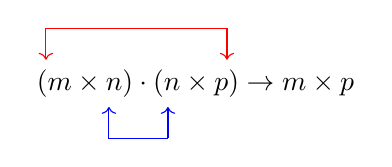
\begin{tikzpicture}
    % The matrix multiplication expression
    \node at (0,0) {\((m \times n) \cdot (n \times p) \rightarrow m \times p\)};
    
    % Red bidirectional U-shaped arrow on top
    \draw[red,<-] (-1.9,0.3) -- (-1.9,0.7) -- (0.4,0.7);
    \draw[red,->] (0.4,0.7) -- (0.4,0.3);
    
    % Blue bidirectional U-shaped arrow on the bottom
    \draw[blue,<-] (-1.1,-0.3) -- (-1.1,-0.7) -- (-0.35,-0.7);
    \draw[blue,->] (-0.35,-0.7) -- (-0.35,-0.3);
\end{tikzpicture}
\]

The diagram shows that the number of columns in the first matrix must equal the number of rows in the second matrix (the \textcolor{blue}{blue arrow}). The result is a new matrix with the number of rows from the first matrix and the number of columns from the second matrix (the \textcolor{red}{red arrow}).

\begin{example}
    For $A$ and $B$ below compute $AB$ and $BA$.

    \[
    A=\left[\begin{array}{lll}
    1 & 2 & -2 \\
    1 & 1 & -3
    \end{array}\right], \quad B=\left[\begin{array}{cccc}
    -4 & 2 & 4 & -4 \\
    -1 & -5 & -3 & 3 \\
    -4 & -4 & -3 & -1
    \end{array}\right]
    \]
    
\end{example}

\begin{solution}
    First $A B=\left[\begin{array}{llll}A \vect{b_1} & A \vect{b_2} & A \vect{b_3} & A \vect{b_4}\end{array}\right]$ :

\[
\begin{aligned}
& A B=\left[\begin{array}{lll}
1 & 2 & -2 \\
1 & 1 & -3
\end{array}\right]\left[\begin{array}{cccc}
-4 & 2 & 4 & -4 \\
-1 & -5 & -3 & 3 \\
-4 & -4 & -3 & -1
\end{array}\right] \\
& = \vcenter{\hbox{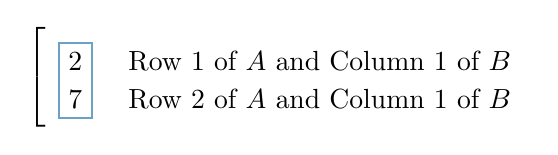
\begin{tikzpicture}
    \matrix (m1) [matrix of math nodes,left delimiter={[}] {
    2 & \quad \text{Row 1 of $A$ and Column 1 of $B$} \\
    7 & \quad \text{Row 2 of $A$ and Column 1 of $B$} \\
    };
    \draw[headercolor,thick] (m1-1-1.north west) rectangle (m1-2-1.south east);
\end{tikzpicture}}} \\
& = \vcenter{\hbox{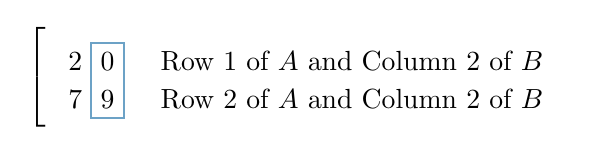
\begin{tikzpicture}
    \matrix (m2) [matrix of math nodes,left delimiter={[}] {
    2 & 0 & \quad \text{Row 1 of $A$ and Column 2 of $B$} \\
    7 & 9 & \quad \text{Row 2 of $A$ and Column 2 of $B$} \\
    };
    \draw[headercolor,thick] (m2-1-2.north west) rectangle (m2-2-2.south east);
\end{tikzpicture}}} \\
& = \vcenter{\hbox{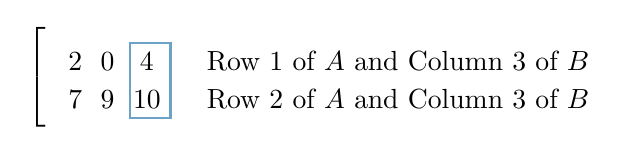
\begin{tikzpicture}
    \matrix (m3) [matrix of math nodes,left delimiter={[}] {
    2 & 0 & 4 & \quad \text{Row 1 of $A$ and Column 3 of $B$} \\
    7 & 9 & 10 & \quad \text{Row 2 of $A$ and Column 3 of $B$} \\
    };
    \draw[headercolor,thick] (m3-1-3.north west) rectangle (m3-2-3.south east);
\end{tikzpicture}}} \\
& = \vcenter{\hbox{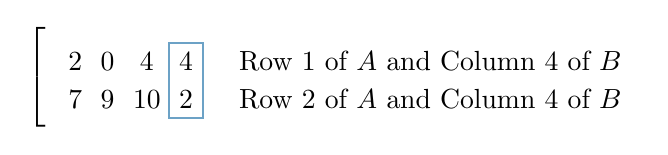
\begin{tikzpicture}
    \matrix (m4) [matrix of math nodes,left delimiter={[}] {
    2 & 0 & 4 & 4 & \quad \text{Row 1 of $A$ and Column 4 of $B$} \\
    7 & 9 & 10 & 2 & \quad \text{Row 2 of $A$ and Column 4 of $B$} \\
    };
    \draw[headercolor,thick] (m4-1-4.north west) rectangle (m4-2-4.south east);
\end{tikzpicture}}} \\
& = \vcenter{\hbox{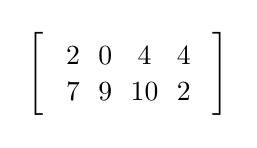
\begin{tikzpicture}
    \matrix (m4) [matrix of math nodes,left delimiter={[}, right delimiter={]}] {
    2 & 0 & 4 & 4 \\
    7 & 9 & 10 & 2 \\
    };
\end{tikzpicture}}}
\end{aligned}
\]

On the other hand, $B A$ is not defined! $B$ has 4 columns and $A$ has 2 rows. Thus, the number of columns in $B$ is not equal to the number of rows in $A$. \end{solution}

\begin{example}
    Example Compute the matrix $A B$, where

\[
A=\left[\begin{array}{ll}
1 & 2 \\
2 & 3 \\
3 & 4
\end{array}\right], \quad \text { and } B=\left[\begin{array}{cc}
2 & -1 \\
3 & 1
\end{array}\right]
\]

\end{example}

\begin{solution}
    By the definition of multiplication given above,

\[
\begin{aligned}
A B & =\left[A\left[\begin{array}{l}
2 \\
3
\end{array}\right] A\left[\begin{array}{c}
-1 \\
1
\end{array}\right]\right] \\
& \left.=\left[\begin{array}{ll}
1 & 2 \\
2 & 3 \\
3 & 4
\end{array}\right]\left[\begin{array}{l}
2 \\
3
\end{array}\right]\left[\begin{array}{ll}
1 & 2 \\
2 & 3 \\
3 & 4
\end{array}\right]\left[\begin{array}{c}
-1 \\
1
\end{array}\right]\right] \\
& =\left[\left[\begin{array}{l}
1 \cdot 2+2 \cdot 3 \\
2 \cdot 2+3 \cdot 3 \\
3 \cdot 2+4 \cdot 3
\end{array}\right]\left[\begin{array}{l}
1 \cdot(-1)+2 \cdot 1 \\
2 \cdot(-1)+3 \cdot 1 \\
3 \cdot(-1)+4 \cdot 1
\end{array}\right]\right] \\
& =\left[\begin{array}{cc}
8 & 1 \\
13 & 1 \\
18 & 1
\end{array}\right]
\end{aligned}
\]
\end{solution}

\begin{example} If $A$ is $3 \times 5$ and $B$ is $5 \times 2$, what are the sizes of $A B$ and $B A$ (assuming they are defined)?
\end{example}

\begin{solution}
    \begin{itemize}
        \item The product $A B$ is defined since the number of columns of $A$ matches the number of rows of $B$ (5). The resulting matrix $A B$ is a $3 \times 2$ matrix.
        \item The product $B A$ is not defined, since the number of columns of $B$ (2) does not match the number of rows of $A$ (3).
    \end{itemize}
\end{solution}

The next example illustrate that even if both $AB$ and $BA$ are defined, they are not necessarily equal.

\begin{example}
    For $A = \left[\begin{array}{rrr}
        -4 & 4 & 3 \\
        3 & -3 & -1 \\
        -2 & -1 & 1
        \end{array}\right] $ and $B = \left[\begin{array}{rrr}
            -1 & -1 & 0 \\
            -3 & 0 & -2 \\
            -2 & 1 & -2
            \end{array}\right]$ compute $AB$ and $BA$.

\end{example}

\begin{solution}
    First $AB$:

    \[
    \begin{aligned}
    A B &=\left[\begin{array}{rrr}
    -4 & 4 & 3 \\
    3 & -3 & -1 \\
    -2 & -1 & 1
    \end{array}\right]\left[\begin{array}{rrr}
    -1 & -1 & 0 \\
    -3 & 0 & -2 \\
    -2 & 1 & -2
    \end{array}\right] \\
    & =\left[\begin{array}{c}
    -14 \\
    8 \\
    3
    \end{array}\right. \\
    & =\left[\begin{array}{rr}
    -14 & 7 \\
    8 & -4 \\
    3 & 3
    \end{array}\right. \\
    & =\left[\begin{array}{rrr}
    -14 & 7 & -14 \\
    8 & -4 & 8 \\
    3 & 3 & 0
    \end{array}\right]
    \end{aligned}
    \]

    Next $BA$:
    \[
    \begin{aligned}
    B A & =\left[\begin{array}{rrr}
    -1 & -1 & 0 \\
    -3 & 0 & -2 \\
    -2 & 1 & -2
    \end{array}\right]\left[\begin{array}{rrr}
    -4 & 4 & 3 \\
    3 & -3 & -1 \\
    -2 & -1 & 1
    \end{array}\right] \\
    & =\left[\begin{array}{rrr}
    1 \\
    16 & \\
    15
    \end{array}\right. \\
    & =\left[\begin{array}{rrr}
    1 & -1 \\
    16 & -10 \\
    15 & -9
    \end{array}\right. \\
    & =\left[\begin{array}{rrr}
    1 & -1 & -2 \\
    16 & -10 & -11 \\
    15 & -9 & -9
    \end{array}\right]
    \end{aligned}
    \]

    We see that $AB \neq BA$. \end{solution}

    In regular arithmetic the multiplicative identity is 1. In matrix algebra, the multiplicative identity is the identity matrix, denoted by $I$. The identity matrix is a \textit{square} matrix with 1s on the diagonal and 0s elsewhere. The size of the identity matrix is determined by the context, and is usually clear from the context. For example, $I_2$ is a $2 \times 2$ identity matrix, and $I_3$ is a $3 \times 3$ identity matrix and in general $I_n \in \mathbb{R}^{n \times n}$ is an $n \times n$ identity matrix:

    $$
    I_n=\left[\begin{array}{ccccc}
    1 & 0 & 0 & \cdots & 0 \\
    0 & 1 & 0 & \cdots & 0 \\
    \vdots & \vdots & \vdots & \cdots & \vdots \\
    0 & 0 & 0 & \cdots & 1
    \end{array}\right]
    $$

    We can now state the following theorem.

    \begin{theorem}
        Let $A, B, C$ be matrices, of appropriate dimensions, and let $\alpha$ be a scalar. Then
\begin{enumerate}[(a)]
    \item $A(BC) = (AB)C$
    \item $A(B + C) = AB + AC$
    \item $(B + C)A = BA + CA$
    \item $\alpha(AB) = (\alpha A)B = A(\alpha B)$
    \item $I_n A = AI_n = A$
\end{enumerate}
\end{theorem}

We conclude this section by looking at the $k$th power of a matrix. \newpage

\begin{definition}
    Let $A$ be a square matrix, i.e. $ A \in \mathbb{R}^{n \times n}$. The $k$th power of $A$, denoted $A^k$, is defined as the product of $A$ with itself $k$ times. That is,

    $$
    A^k=\underbrace{ AAA \cdot \cdots A}_{k \text { times }}
    $$

    where $A$ appears $k$ times on the right-hand side.
\end{definition}

\begin{example}
    Compute $A^3$ if
    \[
    A=\left[\begin{array}{rr}
    -2 & 3 \\
    1 & 0
    \end{array}\right]
    \]
\end{example}

\begin{solution}

    Compute $A^2$ :

    \[
    A^2=\left[\begin{array}{rr}
    -2 & 3 \\
    1 & 0
    \end{array}\right]\left[\begin{array}{rr}
    -2 & 3 \\
    1 & 0
    \end{array}\right]=\left[\begin{array}{rr}
    7 & -6 \\
    -2 & 3
    \end{array}\right]
    \]

    And then $A^3$ :

    \[
    \begin{aligned}
    A^3=A^2 A & =\left[\begin{array}{rr}
    7 & -6 \\
    -2 & 3
    \end{array}\right]\left[\begin{array}{rr}
    -2 & 3 \\
    1 & 0
    \end{array}\right] \\
    & =\left[\begin{array}{rr}
    -20 & 21 \\
    7 & -6
    \end{array}\right]
    \end{aligned}
    \]

    We could also do:

    \[
    A^3=A A^2=\left[\begin{array}{rr}
    -2 & 3 \\
    1 & 0
    \end{array}\right]\left[\begin{array}{rr}
    7 & -6 \\
    -2 & 3
    \end{array}\right]=\left[\begin{array}{rr}
    -20 & 21 \\
    7 & -6
    \end{array}\right]
    \]

\end{solution}

\section{Matrix Transpose}
We begin with the definition of the transpose of a matrix.

\begin{definition}
    Given a matrix $A \in \mathbb{R}^{m \times n}$, the transpose of $A$ is the matrix $A^T$ whose $i$th column is the $i$th row of $A$.
\end{definition}

If $A$ is $m \times n$ then $A^T$ is $n \times m$. For example, if

\[
A=\left[\begin{array}{rrrrr}
0 & -1 & 8 & -7 & -4 \\
-4 & 6 & -10 & -9 & 6 \\
9 & 5 & -2 & -3 & 5 \\
-8 & 8 & 4 & 7 & 7
\end{array}\right]
\]

then

\[
A^T=\left[\begin{array}{rrrr}
0 & -4 & 9 & -8 \\
-1 & 6 & 5 & 8 \\
8 & -10 & -2 & 4 \\
-7 & -9 & -3 & 7 \\
-4 & 6 & 5 & 7
\end{array}\right]
\]

\begin{example} Compute $(AB)^T$ and $B^T A^T$ if

\[
A=\left[\begin{array}{rrr}
-2 & 1 & 0 \\
3 & -1 & -3
\end{array}\right], \quad B=\left[\begin{array}{rrr}
-2 & 1 & 2 \\
-1 & -2 & 0 \\
0 & 0 & -1
\end{array}\right].
\]
\end{example}

\begin{solution}
    First, compute $(AB)^T$:

    \[
    \begin{aligned}
    A B &=\left[\begin{array}{rrr}
    -2 & 1 & 0 \\
    3 & -1 & -3
    \end{array}\right]\left[\begin{array}{rrr}
    -2 & 1 & 2 \\
    -1 & -2 & 0 \\
    0 & 0 & -1
    \end{array}\right] \\
    &=\left[\begin{array}{rrr}
        3 & -4 & -4 \\
        -5 & 5 & 9
        \end{array}\right]
    \end{aligned}
    \]

    and then $(AB)^T$:

    \[
    \begin{aligned}
    (A B)^{T} &=\left[\begin{array}{rrr}
        3 & -4 & -4 \\
        -5 & 5 & 9
        \end{array}\right]^{T} \\
    &=\left[\begin{array}{rr}
        3 & -5 \\
        -4 & 5 \\
        -4 & 9
        \end{array}\right]
    \end{aligned}
    \]

    Next, compute $B^T A^T$:

    \[
    \begin{aligned}
    B^{T} A^{T} &=\left[\begin{array}{rrr}
        -2 & -1 & 0 \\
        1 & -2 & 0 \\
        2 & 0 & -1
        \end{array}\right]\left[\begin{array}{rr}
        -2 & 3 \\
        1 & -1 \\
        0 & -3
        \end{array}\right] \\
    &=\left[\begin{array}{rr}
    3 & -5 \\
    -4 & 5 \\
    -4 & 9
    \end{array}\right]
    \end{aligned}
    \]

    We see that $(AB)^T = B^T A^T$. \end{solution}

The following theorem summarises the properties of the transpose of a matrix.

\begin{theorem}
    Let $A$ and $B$ be matrices of appropriate dimensions and let $\alpha$ be a scalar. Then
    \begin{enumerate}[(a)]
        \item $(A^T)^T = A$
        \item $(A + B)^T = A^T + B^T$
        \item $(\alpha A)^T = \alpha A^T$
        \item $(AB)^T = B^T A^T$
    \end{enumerate}
\end{theorem}

A consequence of property (4) is that
\[
\left(A_1 A_2 \ldots A_k\right)^T=A_k^T A_{k-1}^T \cdots A_2^T A_1^T
\]

and as a special case

\[
\left(A^k\right)^T=\left(A^T\right)^k
\]

\section{Invertible Matrices}
The inverse of a square matrix \( A \in \mathbb{R}^{n \times n} \) extends the concept of the reciprocal for a nonzero real number \( a \in \mathbb{R} \). More precisely, the inverse of a non-zero number \( a \in \mathbb{R} \) is the unique number \( c \in \mathbb{R} \) such that \( a c = c a = 1 \). The inverse of \( a \neq 0 \), typically written as \( a^{-1} = \frac{1}{a} \), enables solving the equation \( a x = b \):

\[
a x = b \Rightarrow a^{-1} a x = a^{-1} b \Rightarrow x = a^{-1} b.
\]

This concept extends to square matrices, where the inverse of a matrix \( A \in \mathbb{R}^{n \times n} \) is a matrix \( C \in \mathbb{R}^{n \times n} \) such that \( A C = C A = I_n \), where \( I_n \) is the identity matrix of size \( n \times n \). The inverse of a matrix is denoted by \( A^{-1} \). We can now define the invertible matrix.

\begin{definition}
    A square matrix \( A \in \mathbb{R}^{n \times n} \) is invertible (or \textbf{nonsingular}) if there exists a matrix \( C \in \mathbb{R}^{n \times n} \) such that \( A C = C A = I_n \). The matrix \( C \) is called the inverse of \( A \) and is denoted by \( A^{-1} \). Thus, \( A^{-1} A = A A^{-1} = I_n \).
\end{definition}

\begin{example}
    Given $A$ and $C$ below, show that $C$ is the inverse of $A$.

    \[
    A=\left[\begin{array}{rrr}
    1 & -3 & 0 \\
    -1 & 2 & -2 \\
    -2 & 6 & 1
    \end{array}\right], \quad C=\left[\begin{array}{rrr}
    -14 & -3 & -6 \\
    -5 & -1 & -2 \\
    2 & 0 & 1
    \end{array}\right]
    \]
    \label{ex:inverse2}
\end{example}

\begin{solution}
    We need to show that $A C = C A = I_3$. First, compute $AC$:

    \[
    \begin{aligned}
    A C &=\left[\begin{array}{rrr}
    1 & -3 & 0 \\
    -1 & 2 & -2 \\
    -2 & 6 & 1
    \end{array}\right]\left[\begin{array}{rrr}
    -14 & -3 & -6 \\
    -5 & -1 & -2 \\
    2 & 0 & 1
    \end{array}\right] \\
    &=\left[\begin{array}{rrr}
    1 & 0 & 0 \\
    0 & 1 & 0 \\
    0 & 0 & 1
    \end{array}\right]=I_3
    \end{aligned}
    \]

    Next, compute $CA$:

    \[
    \begin{aligned}
    C A &=\left[\begin{array}{rrr}
    -14 & -3 & -6 \\
    -5 & -1 & -2 \\
    2 & 0 & 1
    \end{array}\right]\left[\begin{array}{rrr}
    1 & -3 & 0 \\
    -1 & 2 & -2 \\
    -2 & 6 & 1
    \end{array}\right] \\
    &=\left[\begin{array}{rrr}
    1 & 0 & 0 \\
    0 & 1 & 0 \\
    0 & 0 & 1
    \end{array}\right]=I_3
    \end{aligned}
    \]

    We see that $C=A^{-1}$ is the inverse of $A$. \end{solution}

The following theorem summarizes the relationship between the matrix inverse and matrix multiplication and matrix transpose.

\begin{theorem} Let $A$ and $B$ be invertible $n \times n$ matrices. Then:
\begin{enumerate}[(a)]
    \item $A^{-1}$ is invertible, with
    \[
    \left(A^{-1}\right)^{-1}=A
    \]
    \item The product $A B$ is invertible, with
    \[
    (A B)^{-1}=B^{-1} A^{-1}
    \]
    \item The transpose of $A$ is also invertible, i.e. $A^T$ is invertible, with
    \[
    \left(A^T\right)^{-1}=\left(A^{-1}\right)^T
    \]
\end{enumerate}

\end{theorem}

We will now consider how we can find the inverse of a matrix.

\subsection*{Finding the Determinant and Inverse of a $2 \times 2$ Matrix}

The inverse of a matrix is not always easy to find. However, for a $2 \times 2$ matrix, we can use a formula to find the inverse.

\begin{theorem}
    Let $A=\left[\begin{array}{ll}
    a & b \\
    c & d
    \end{array}\right]$. If $ad-bc \neq 0$, then the inverse of $A$ is given by

    \[
    A^{-1}=\frac{1}{ad-bc}\left[\begin{array}{cc}
    d & -b \\
    -c & a
    \end{array}\right]
    \]
\end{theorem}

\begin{remark}
    The quantity $ad - bc$ is called the determinant of $A$, and we write
    \[
    \text{det}(A) = |A| = ad - bc
    \]
\end{remark}

The determinant of a $2 \times 2$ matrix is a scalar quantity that provides information about the matrix. If the determinant is zero, then the matrix is not invertible. If the determinant is non-zero, then the matrix is invertible. These formulae are only valid $2 \times 2$ matrices.

\begin{example} We let

\[
A=\left[\begin{array}{ll}
1 & 2 \\
3 & 4
\end{array}\right]
\]

and compute $A^{-1}$. By the theorem, we have

\[
\begin{aligned}
A^{-1} & =\frac{1}{1 \cdot 4-2 \cdot 3}\left[\begin{array}{cc}
4 & -2 \\
-3 & 1
\end{array}\right] \\
& =-\frac{1}{2}\left[\begin{array}{cc}
4 & -2 \\
-3 & 1
\end{array}\right] \\
& =\left[\begin{array}{cc}
-2 & 1 \\
\frac{3}{2} & -\frac{1}{2}
\end{array}\right]
\end{aligned}
\]

Now we confirm that $A A^{-1}=I_2$ :

\[
\begin{aligned}
A A^{-1} & =\left[\begin{array}{ll}
1 & 2 \\
3 & 4
\end{array}\right]\left[\begin{array}{cc}
-2 & 1 \\
\frac{3}{2} & -\frac{1}{2}
\end{array}\right] \\
& =\left[\begin{array}{ll}
1(-2)+2\left(\frac{3}{2}\right) & 1(1)+2\left(-\frac{1}{2}\right) \\
3(-2)+4\left(\frac{3}{2}\right) & 3(1)+4\left(-\frac{1}{2}\right)
\end{array}\right] \\
& =\left[\begin{array}{ll}
-2+3 & 1-1 \\
-6+6 & 3-2
\end{array}\right] \\
& =\left[\begin{array}{ll}
1 & 0 \\
0 & 1
\end{array}\right]
\end{aligned}
\]
\label{ex:inverse}
\end{example}

\begin{example} Find the inverse of $A=\left[\begin{array}{cc}1 & 3 \\ -1 & -2\end{array}\right]$ if it exists.
    
\end{example}

\begin{solution}
    We first compute the determinant of $A$:

    \[
    \text{det}(A)=1(-2)-3(-1)=(-2)+3=1
    \]

    Since the determinant is non-zero, the inverse of $A$ exists. By the formula, we have

    \[
    \begin{aligned}
    A^{-1} & =\frac{1}{1}\left[\begin{array}{cc}-2 & -3 \\ 1 & 1\end{array}\right]
    \end{aligned}
    \]

    We can confirm that $A A^{-1}=I_2$:

    \[
        A A^{-1}=\left[\begin{array}{cc}
    1 & 3 \\
    -1 & -2
    \end{array}\right]\left[\begin{array}{cc}
    -2 & -3 \\
    1 & 1
    \end{array}\right]=\left[\begin{array}{ll}
    1 & 0 \\
    0 & 1
    \end{array}\right] =I_2
    \]

\end{solution}

For larger matrices, we need to use other methods to find the inverse.

\subsection*{Finding the Inverse of a $n \times n$ Matrix}
An \textbf{elementary matrix} is a matrix that is obtained by performing a single elementary row operation (replacement, swap, or scaling) on an identity matrix. For example, the matrix

\[
E_1=\left[\begin{array}{ccc}
1 & 0 & 0 \\
0 & 1 & 0 \\
-2 & 0 & 1
\end{array}\right]
\]

is an elementary matrix since it is obtained from $I_3$ via the single elementary row operation $r_3 \mapsto r_3-2 r_1$.

\begin{example}

Let $A$ be a general $3 \times 3$ matrix

\[
A=\left[\begin{array}{lll}
a & b & c \\
d & e & f \\
g & h & i
\end{array}\right]
\]

and we let $E_1, E_2$, and $E_3$ be the elementary matrices

\[
E_1=\left[\begin{array}{ccc}
1 & 0 & 0 \\
0 & 1 & 0 \\
-2 & 0 & 1
\end{array}\right], \quad E_2=\left[\begin{array}{lll}
1 & 0 & 0 \\
0 & 0 & 1 \\
0 & 1 & 0
\end{array}\right], \quad \text { and } \quad E_3=\left[\begin{array}{lll}
1 & 0 & 0 \\
0 & 3 & 0 \\
0 & 0 & 1
\end{array}\right]
\]
\end{example}

Notice, then, that $E_1$ corresponds to $r_3 \mapsto r_3-2 r_1, E_2$ corresponds to $r_2 \longleftrightarrow r_3$, and $E_3$ corresponds to $r_2 \mapsto 3 r_2$. We also have the following products:

\[
E_1 A=\left[\begin{array}{ccc}
a & b & c \\
d & e & f \\
g-2 a & h-2 b & i-2 c
\end{array}\right], \quad E_2 A=\left[\begin{array}{ccc}
a & b & c \\
g & h & i \\
d & e & f
\end{array}\right], \quad \text { and } \quad E_3 A=\left[\begin{array}{ccc}
a & b & c \\
3 d & 3 e & 3 f \\
g & h & i
\end{array}\right] .
\]


Notice that $E_1 A$ is the matrix obtained by performing the row operation $r_3 \mapsto r_3-2 r_1$ on $A$. In general, multiplying $A$ on the left by an elementary matrix is the same as performing the corresponding row operation on $A$. We can also represent a sequence of row operations by multiplication of several elementary matrices. For example,

\[
E_2 E_1 A=\left[\begin{array}{ccc}
a & b & c \\
g-2 a & h-2 b & i-2 c \\
d & e & f
\end{array}\right]
\]

corresponds to performing $r_3 \mapsto r_3-2 r_1$ followed by $r_2 \longleftrightarrow r_3$ on the matrix $A$.
As we have observed before, row operations are reversible. It follows that elementary matrices are also invertible. This leads to the following theorem.

\begin{theorem}
    An $n \times n$ matrix $A$ is invertible if and only if $A$ is row equivalent to $I_n$. In this case, any sequence of elementary row operations that reduces $A$ to $I_n$ also transforms $I_n$ into $A^{-1}$.
\end{theorem}

This theorem leads to a nice algorithm for finding the inverse of an $n \times n$ matrix, assuming such an inverse exists.

\begin{custombox}{Algorithm for Finding the Inverse of an $n \times n$ Matrix}
    Let $A$ be an $n \times n$ matrix. To find the inverse of $A$, follow these steps:
    \begin{enumerate}
        \item Form the augmented matrix $[A | I_n]$.
        \item Perform row operations on $[A | I_n]$ to reduce $A$ to $I_n$.
        \item The matrix on the right side of the augmented matrix is $A^{-1}$.
    \end{enumerate}

    If $A$ is not invertible, then the algorithm will not be able to reduce $A$ to $I_n$.
\end{custombox}

\begin{example} Find the inverse of $A=\left[\begin{array}{rrr}1 & 0 & 3 \\ 1 & 1 & 0 \\ -2 & 0 & -7\end{array}\right]$ if it exists.    
\end{example}

\begin{solution}
    Solution. Form the augmented matrix $\left[\begin{array}{ll}A & I_3\end{array}\right]$ and row reduce:
\[
\begin{alignedat}{3}
& \left[\begin{array}{cccccc}
1 & 0 & 3 & 1 & 0 & 0 \\
1 & 1 & 0 & 0 & 1 & 0 \\
-2 & 0 & -7 & 0 & 0 & 1
\end{array}\right]
& \quad & \begin{aligned}
    r_2 &\mapsto -r_1 + r_2 \\
    r_3 &\mapsto 2 r_1 + r_3
\end{aligned}
& \quad & \left[\begin{array}{cccccc}
1 & 0 & 3 & 1 & 0 & 0 \\
0 & 1 & -3 & -1 & 1 & 0 \\
0 & 0 & -1 & 2 & 0 & 1
\end{array}\right] \\[10pt]
& & \quad & r_3 \mapsto -r_3
& \quad & \left[\begin{array}{cccccc}
1 & 0 & 3 & 1 & 0 & 0 \\
0 & 1 & -3 & -1 & 1 & 0 \\
0 & 0 & 1 & -2 & 0 & -1
\end{array}\right] \\[10pt]
& & \quad & \begin{aligned}
    r_2 &\mapsto 3 r_3 + r_2 \\
    r_1 &\mapsto -3 r_3 + r_1
\end{aligned}
& \quad & \left[\begin{array}{cccccc}
1 & 0 & 0 & 7 & 0 & 3 \\
0 & 1 & 0 & -7 & 1 & -3 \\
0 & 0 & 1 & -2 & 0 & -1
\end{array}\right]
\end{alignedat}
\]

Therefore, \(\operatorname{rref}A = I_3\), confirming that \( A \) is invertible. The inverse is
\[
A^{-1} = \left[\begin{array}{ccc}
7 & 0 & 3 \\
-7 & 1 & -3 \\
-2 & 0 & -1
\end{array}\right]
\]
Verify:
\[
AA^{-1}=\left[\begin{array}{ccc}
1 & 0 & 3 \\
1 & 1 & 0 \\
-2 & 0 & -7
\end{array}\right]\left[\begin{array}{ccc}
7 & 0 & 3 \\
-7 & 1 & -3 \\
-2 & 0 & -1
\end{array}\right]=\left[\begin{array}{lll}
1 & 0 & 0 \\
0 & 1 & 0 \\
0 & 0 & 1
\end{array}\right]
\]

\end{solution}

\begin{example}
    Find the inverse of $A=\left[\begin{array}{rrr}1 & 0 & 1 \\ 1 & 1 & -2 \\ -2 & 0 & -2\end{array}\right]$ if it exists.
\end{example}

\begin{solution}
    Form the augmented matrix $\left[\begin{array}{ll}A & I_3\end{array}\right]$ and row reduce:
\[
\begin{alignedat}{3}
& \left[\begin{array}{cccccc}
1 & 0 & 1 & 1 & 0 & 0 \\
1 & 1 & -2 & 0 & 1 & 0 \\
-2 & 0 & -2 & 0 & 0 & 1
\end{array}\right]
& \quad & \begin{aligned}
    r_2 &\mapsto -r_1 + r_2 \\
    r_3 &\mapsto 2 r_1 + r_3
\end{aligned}
& \quad & \left[\begin{array}{cccccc}
1 & 0 & 1 & 1 & 0 & 0 \\
0 & 1 & -3 & -1 & 1 & 0 \\
0 & 0 & 0 & 2 & 0 & 1
\end{array}\right]
\end{alignedat}
\]

We need not go further since the rref($A$) is not $I_3$. Therefore, A is not invertible.
\end{solution}

\begin{example}
    Find the inverse of the matrix

    \[
    A=\left[\begin{array}{lll}
        1 & 2 & 1 \\
        4 & 5 & 3 \\
        0 & 0 & 2
        \end{array}\right]
    \]
if it exists.
\end{example}

\begin{solution} (We ommit the row reduction steps for brevity.)
\[
\begin{aligned}
{\left[\begin{array}{llllll}
1 & 2 & 1 & 1 & 0 & 0 \\
4 & 5 & 3 & 0 & 1 & 0 \\
0 & 0 & 2 & 0 & 0 & 1
\end{array}\right] } & \sim\left[\begin{array}{cccccc}
1 & 2 & 1 & 1 & 0 & 0 \\
0 & -3 & -1 & -4 & 1 & 0 \\
0 & 0 & 2 & 0 & 0 & 1
\end{array}\right] \\
& \sim\left[\begin{array}{cccccc}
1 & 2 & 1 & 1 & 0 & 0 \\
0 & -3 & -1 & -4 & 1 & 0 \\
0 & 0 & 1 & 0 & 0 & \frac{1}{2}
\end{array}\right] \\
& \sim\left[\begin{array}{cccccc}
1 & 2 & 0 & 1 & 0 & -\frac{1}{2} \\
0 & -3 & 0 & -4 & 1 & \frac{1}{2} \\
0 & 0 & 1 & 0 & 0 & \frac{1}{2}
\end{array}\right] \\
& \sim\left[\begin{array}{cccccc}
1 & 2 & 0 & 1 & 0 & -\frac{1}{2} \\
0 & 1 & 0 & \frac{4}{3} & -\frac{1}{3} & -\frac{1}{6} \\
0 & 0 & 1 & 0 & 0 & \frac{1}{2}
\end{array}\right] \\
& \sim\left[\begin{array}{cccccc}
1 & 0 & 0 & -\frac{5}{3} & \frac{2}{3} & -\frac{1}{6} \\
0 & 1 & 0 & \frac{4}{3} & -\frac{1}{3} & -\frac{1}{6} \\
0 & 0 & 1 & 0 & 0 & \frac{1}{2}
\end{array}\right] .
\end{aligned}
\]

Hence

\[
A^{-1}=\left[\begin{array}{ccc}
-\frac{5}{3} & \frac{2}{3} & -\frac{1}{6} \\
\frac{4}{3} & -\frac{1}{3} & -\frac{1}{6} \\
0 & 0 & \frac{1}{2}
\end{array}\right] .
\]

\end{solution}

With the method for finding matrix inverses established, we now have a powerful tool for approaching linear systems. We will see how matrix inverses can be used to solve systems of equations efficiently, offering a straightforward way to find solutions when a matrix is invertible.

\subsection*{Solving Matrix Equations with Inverses}
Just like we can solve an equation by using the reciprocal of a non-zero number as we saw previously, we can do something similar with matrices. When a matrix \( A \) is invertible, we can use its inverse to solve matrix equations involving \( A \). This brings us to the theorem below, which shows how we can find solutions for equations like \( A \vect{x} = \vect{b} \) when \( A \) has an inverse.

\begin{theorem}
    Let \( A \) be an invertible matrix. Then the equation \( A \vect{x} = \vect{b} \) has a unique solution given by \( \vect{x} = A^{-1} \vect{b} \).
\end{theorem}

\begin{example}
We can use the inverse from example \ref{ex:inverse} to solve the linear system

\[
\begin{aligned}
x_1+2 x_2 & =5 \\
3 x_1+4 x_2 & =6 .
\end{aligned}
\]

We think of this in matrix terms as \(A \vect{x}=\vect{b}\), where

\[
A=\left[\begin{array}{ll}
1 & 2 \\
3 & 4
\end{array}\right], \quad \vect{x}=\left[\begin{array}{l}
x_1 \\
x_2
\end{array}\right], \quad \text { and } \quad \vect{b}=\left[\begin{array}{l}
5 \\
6
\end{array}\right]
\]

The theorem tells us that \(\vect{x}=A^{-1} \vect{b}\) is a solution, i.e. that

\[
\begin{aligned}
{\left[\begin{array}{l}
x_1 \\
x_2
\end{array}\right] } & =\left[\begin{array}{cc}
-2 & 1 \\
\frac{3}{2} & -\frac{1}{2}
\end{array}\right]\left[\begin{array}{l}
5 \\
6
\end{array}\right] \\
& =\left[\begin{array}{c}
-2(5)+1(6) \\
\frac{3}{2}(5)-\frac{1}{2}(6)
\end{array}\right] \\
& =\left[\begin{array}{c}
-4 \\
\frac{9}{2}
\end{array}\right]
\end{aligned}
\]
\end{example}

\begin{example} Use the result from example \ref{ex:inverse2} to solve the linear system $A \vect{x} = \vect{b}$ where

    \[A=\left[\begin{array}{rrr}1 & -3 & 0 \\ -1 & 2 & -2 \\ -2 & 6 & 1\end{array}\right], \quad \vect{b}=\left[\begin{array}{c}1 \\ -3 \\ -1\end{array}\right]\]

\end{example}

\begin{solution} We showed in example \ref{ex:inverse2} that

    \[
    A^{-1}=\left[\begin{array}{rrr}
    -14 & -3 & -6 \\
    -5 & -1 & -2 \\
    2 & 0 & 1
    \end{array}\right]
    \]

Therefore, the unique solution to the linear system $A \vect{x} = \vect{b}$ is

    \[
    A^{-1} \vect{b}=\left[\begin{array}{rrr}
    -14 & -3 & -6 \\
    -5 & -1 & -2 \\
    2 & 0 & 1
    \end{array}\right]\left[\begin{array}{c}
    1 \\
    -3 \\
    -1
    \end{array}\right]=\left[\begin{array}{l}
    1 \\
    0 \\
    1
    \end{array}\right]
    \]

Verify:

    \[
    \left[\begin{array}{rrr}
    1 & -3 & 0 \\
    -1 & 2 & -2 \\
    -2 & 6 & 1
    \end{array}\right]\left[\begin{array}{l}
    1 \\
    0 \\
    1
    \end{array}\right]=\left[\begin{array}{c}
    1 \\
    -3 \\
    -1
    \end{array}\right]
    \]
\end{solution}

We conclude this chapter with one of the most important theorems in linear algebra, The Invertible Matrix Theorem.

\section{The Invertible Matrix Theorem}

The Invertible Matrix Theorem provides a comprehensive list of equivalent statements for a square matrix to be invertible and it enables us to determine the truth value of one statement by checking the truth value of another.

\newpage

\begin{theorem}
    Let \( A \) be an \( n \times n \) matrix. The following statements are equivalent:
    \begin{enumerate}[(a)]
        \item $A$ is invertible.
        \item $A$ is row equivalent to $I_n$.
        \item $A$ has $n$ pivot positions (i.e. one for each row and column).
        \item The equation $A \vect{x}=\overline{0}$ has only the trivial solution.
        \item The columns of $A$ are linearly independent.
        \item The equation \( A \vect{x} = \vect{b} \) has a unique solution for each \( \vect{b} \in \mathbb{R}^n \).
        \item The columns of $A \operatorname{span} \mathbb{R}^n$.
        \item \( \text{det}(A) \neq 0 \).
        \item There is an $n \times n$ matrix $C$ such that $C A=I$.
        \item There is an $n \times n$ matrix $D$ such that $A D=I$.
        \item $A^T$ is invertible.
    \end{enumerate}
\end{theorem}

Note how the theorem connects the properties of a matrix to its invertibility, thus summarising the main elements of our discussion on linear systems, independence, vectors, and matrices.

\begin{example} Decide if the following matrix is invertible:

\[
A=\left[\begin{array}{lll}
2 & 2 & 2 \\
1 & 3 & 1 \\
4 & 4 & 6
\end{array}\right]
\]

\end{example}

\begin{solution}
Performing row operations, we see

\[
\begin{aligned}
A & \sim\left[\begin{array}{lll}
1 & 3 & 1 \\
2 & 2 & 2 \\
4 & 4 & 6
\end{array}\right] \\
& \sim\left[\begin{array}{ccc}
1 & 3 & 1 \\
0 & -4 & 0 \\
0 & -8 & 2
\end{array}\right] \\
& \sim\left[\begin{array}{ccc}
1 & 3 & 1 \\
0 & -4 & 0 \\
0 & 0 & 2
\end{array}\right]
\end{aligned}
\]
which has 3 pivots, so by (c) we have that $A$ is invertible.
\end{solution}

This concludes our discussion on matrices.
% \chapter{Differential Calculus}
\label{chap:ch10}

In both practical experience and modern engineering, we frequently encounter situations where one quantity changes in response to another. A car’s fuel consumption reflects how distance depends on the amount of fuel used. A sprinter’s velocity describes how position varies with time. In agriculture, yield changes with the amount of fertiliser, and in economics, demand responds to price. The study of such relationships lies at the heart of \emph{differential calculus}, the mathematical discipline devoted to understanding how quantities vary together.

The concept that captures this variation is the \emph{rate of change}.

\begin{itemize}
\item The change of distance with respect to time is \emph{velocity}.
\item The change of profit with respect to price is \emph{marginal profit}.
\item The change of loss with respect to model parameters is the \emph{gradient}.
\end{itemize}

When a rate of change remains constant, the relationship between the quantities is linear, and the graph forms a straight line. When the rate of change varies, the graph becomes curved, and the slope depends on the specific point of measurement. This naturally leads to the idea of a \emph{tangent line}, which locally approximates a curve at a single point.

% --- Ensure these packages are in your preamble ---
% \usepackage{pgfplots}
% \usepackage{xcolor}
% \pgfplotsset{compat=1.17}

% --- Ensure your custom color is defined ---
% \definecolor{mseViaBlue}{HTML}{1933CC}

\begin{figure}[htbp]
    \centering
    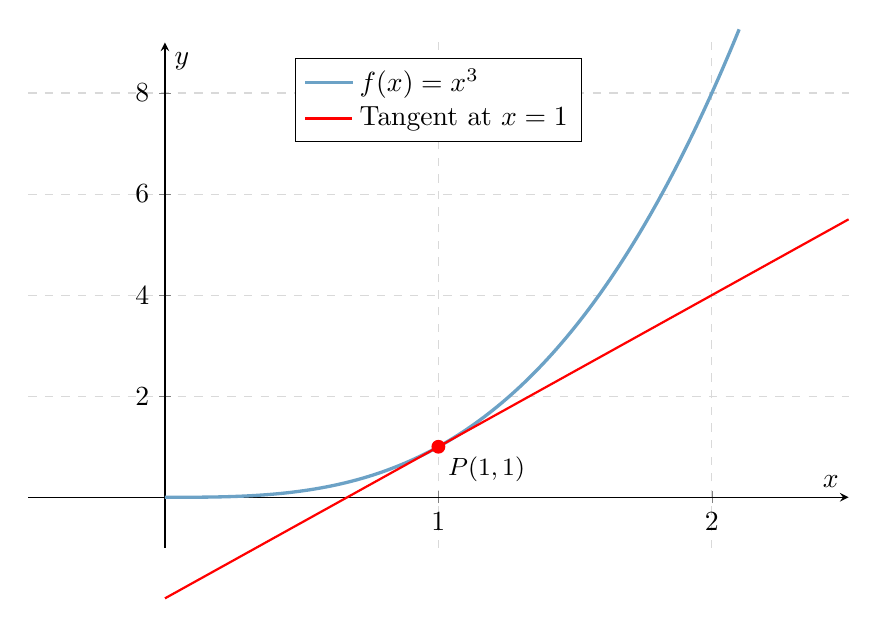
\begin{tikzpicture}
        \begin{axis}[
            axis lines=middle,
            xlabel=$x$,
            ylabel=$y$,
            width=12cm, height=8cm,
            xmin=-0.5, xmax=2.5,
            ymin=-1, ymax=9,
            xtick={-1, 0, 1, 2},
            ytick={0, 2, 4, 6, 8},
            grid=major,
            grid style={dashed, gray!30},
            legend style={
                at={(0.5, 0.97)}, % Position near the top center
                anchor=north,     % Anchor the top-center of the legend box
                legend cell align={left}
            },
            clip=false
        ]
        % Plot the curve f(x) = x^3
        \addplot[
            domain=0:2.1, samples=100,
            smooth, very thick, mseViaBlue
        ] {x^3};
        \addlegendentry{\(f(x) = x^3\)}

        % Plot the tangent line at x=1, which is y = 3x - 2
        \addplot[
            domain=0:2.5,
            red, thick
        ] {3*x - 2};
        \addlegendentry{Tangent at \(x=1\)}

        % Mark the point of tangency
        \coordinate (P) at (axis cs:1, 1);
        \fill[red] (P) circle (2.5pt);
        \node[below right, font=\small] at (P) {\(P(1, 1)\)};
        
        \end{axis}
    \end{tikzpicture}
    \caption{The tangent line to the graph of \(f(x)=x^3\) at the point \(P(1, 1)\).}
    \label{fig:ch10-tangent}
\end{figure}

\begin{remark}
For a straight line, the slope is constant. For a curved graph, the slope varies from point to point, so we speak of the \emph{instantaneous rate of change}, the slope of the tangent at a specific point.
\end{remark}

The same principle extends to computational and data-driven systems. A program’s runtime changes with input size, a model’s accuracy varies with the number of training epochs, and network throughput depends on available bandwidth. In machine learning, the process of training a model resembles a hiker searching for the lowest point in a vast, foggy landscape. The “altitude” represents the model’s error, and progress requires moving downhill. Determining the correct direction among millions of possible ones depends on knowing the local slope — the \emph{derivative} — which expresses the instantaneous rate of change.

Differential calculus provides the tools to describe, compute, and interpret such changes with precision. It transforms intuitive ideas such as being faster, steeper, or more efficient into exact mathematical expressions. This chapter introduces the fundamental ideas of differential calculus, beginning with the concepts of \emph{limits} and \emph{continuity}, which formalise the notion of approaching a point infinitely closely. Building on these, we develop the definition and interpretation of the \emph{derivative} as a measure of instantaneous change and explore its applications in contexts ranging from physical motion to the optimisation of modern algorithms.


\section{Limits and Continuity: The Foundation of Calculus}

Before we can measure an instantaneous rate of change, we must first build a formal understanding of what it means to get "infinitesimally close" to a point without necessarily being at that point. This is the concept of a \textbf{limit}. Building on limits, \textbf{continuity} gives us the language to describe functions that are predictable and well-behaved, without sudden jumps or breaks.

\subsection*{Limits}

A limit describes the value that a function "approaches" as its input gets closer and closer to a specific point. This idea is fundamental not just in calculus, but in software engineering, where we often analyze the behavior of systems under approaching conditions.

For example, when analyzing an algorithm's runtime, we ask what happens to the execution time as the input size `n` approaches infinity. In networking, we might model the theoretical maximum throughput as a limit when latency approaches zero.

\begin{definition}[Limit]
Let \( f(x) \) be a function defined near a point \( c \). We say that the \textbf{limit} of \( f(x) \) as \( x \) approaches \( c \) is \( L \), written as
\vspace{0.5em}
\[
\lim_{x \to c} f(x) = L
\]
\vspace{0.5em}
if we can make the value of \( f(x) \) arbitrarily close to \( L \) by choosing an \( x \) that is sufficiently close to \( c \), but not equal to \( c \).
\end{definition}

In many simple cases, the limit is just the value of the function at that point. For example, for \( f(x) = x^2 \), the limit as \( x \) approaches 3 is simply \( 3^2 = 9 \). The real power of limits, however, is in handling cases where the function is undefined at the point of interest.

\begin{example} A Limit at an Undefined Point

Consider the function \( f(x) = \frac{\sin(x)}{x} \). This function is fundamental in signal processing and is known as the sinc function. Notice that \( f(0) \) is undefined because it results in division by zero. However, we can ask what value the function approaches as \( x \) gets very close to 0.

By plugging in values very close to 0, we can observe a trend:
\begin{align*}
f(0.1) &= \frac{\sin(0.1)}{0.1} \approx 0.9983 \\
f(0.01) &= \frac{\sin(0.01)}{0.01} \approx 0.99998 \\
f(-0.01) &= \frac{\sin(-0.01)}{-0.01} \approx 0.99998
\end{align*}
The function appears to approach 1. In calculus, it can be formally proven that:
\[
\lim_{x \to 0} \frac{\sin(x)}{x} = 1
\]
This ability to analyze behavior at a problematic point is essential for creating robust numerical algorithms.
\end{example}

\begin{example} Asymptotic Analysis with Limits

Suppose you want to analyze whether the function \( f(n) = 5n^2 + 4n + 7 \) is \( \mathcal{O}(n^2) \) as \( n \) grows large, as is common in the study of algorithm complexity. One way to formalize this is to examine the limit:
\[
\lim_{n \to \infty} \frac{f(n)}{n^2}
= \lim_{n \to \infty} \frac{5n^2 + 4n + 7}{n^2}
= \lim_{n \to \infty} \left( 5 + \frac{4}{n} + \frac{7}{n^2} \right)
\]
As \( n \) becomes very large, the terms \( \frac{4}{n} \) and \( \frac{7}{n^2} \) both approach zero, so the whole expression approaches \( 5 \). Because this limit is a finite constant, it confirms that \( f(n) \) grows at the same rate as \( n^2 \). This type of limit calculation is at the heart of asymptotic analysis, formally justifying Big-\(\mathcal{O}\) claims about algorithm runtime.
\end{example}

\subsection*{Continuity}
Continuity formalizes the idea of a function being "well-behaved" or predictable. Intuitively, a function is continuous if you can draw its graph without lifting your pen from the paper. In software, we often assume our systems are continuous: a small change in input should lead to a small, predictable change in output, not a sudden, drastic jump.

\begin{definition}[Continuity]
A function \( f \) is \textbf{continuous} at a point \( c \) if the following three conditions are met:
\begin{enumerate}
    \item \( f(c) \) is defined.
    \item \( \lim_{x \to c} f(x) \) exists.
    \item \( \lim_{x \to c} f(x) = f(c) \).
\end{enumerate}
A function is continuous on an interval if it is continuous at every point in that interval.
\end{definition}

Discontinuities often represent important events in software systems, such as state transitions or threshold triggers.

\begin{example} Jump Discontinuity in a SaaS Pricing Model
    
Consider a cloud service that charges based on the number of API calls per month. The pricing model is tiered: \$20 for up to 10,000 calls, and \$40 for any usage above 10,000 calls. The cost function \(C(x)\), where \(x\) is the number of calls, has a \textbf{jump discontinuity} at \(x = 10,000\).
\[
C(x) =
\begin{cases}
    20 & \text{if } x \le 10000 \\
    40 & \text{if } x > 10000
\end{cases}
\]
As shown in \autoref{fig:jump_discontinuity}, the cost suddenly jumps at the threshold. Understanding discontinuities is crucial for modeling any system with threshold-based logic, from auto-scaling policies to billing systems.
\end{example}

\begin{figure}[htbp]
\centering
\begin{tikzpicture}
\begin{axis}[
    xlabel={API Calls},
    ylabel={Cost (\$)},
    xmin=0, xmax=20,
    ymin=0, ymax=50,
    xtick={0, 10, 20},
    xticklabels={0, 10k, 20k},
    ytick={0, 20, 40},
    grid=major,
    grid style={dashed,gray!30},
    title style={font=\bfseries}
]
% First tier: C(x) = 20 for x <= 10000
\addplot[mseViaBlue, very thick, domain=0:10] {20};
% Second tier: C(x) = 40 for x > 10000
\addplot[mseViaBlue, very thick, domain=10:20] {40};

% Mark the discontinuity
% Solid circle at the end of the first tier
\addplot[only marks, mark=*, mark size=2pt, mseViaBlue] coordinates {(10, 20)};
% Hollow circle at the start of the second tier
\addplot[only marks, mark=o, mark size=2pt, mseViaBlue, thick] coordinates {(10, 40)};
\end{axis}
\end{tikzpicture}
\caption{The cost function exhibits a jump discontinuity at 10,000 API calls as the price tier changes.}
\label{fig:jump_discontinuity}
\end{figure}

\section{The Derivative: Measuring the Rate of Change}
\label{sec:ch10-derivative}

We often talk about average rates of change. For example, if a data transfer takes 10 seconds and moves 500 MB, the average transfer rate is 50 MB/s. But this average tells us nothing about fluctuations during the transfer. The \textbf{derivative} is the tool that lets us move from this average rate to the \textbf{instantaneous rate of change} at any specific moment.

We may thus say that differential calculus is about determining how one quantity changes in relation to another. Geometrically, the derivative of a function at a point is the slope of the line tangent to the function's graph at that point. To find the slope of a tangent, we approximate it using secant lines between two nearby points on the curve. As the points move closer together, the secant slope approaches the tangent slope. As shown in \autoref{fig:secant_to_tangent}, this tangent line is the limit of secant lines passing through two points on the curve as the points get infinitesimally close.

\begin{figure}[htbp]
    \centering
    \begin{tikzpicture}
    \begin{axis}[
        axis lines=middle, xlabel={$x$}, ylabel={$y$},
        xtick=\empty, ytick=\empty,
        xmin=-0.5, xmax=3, ymin=-0.5, ymax=9,
        width=14cm, height=10cm,
        legend style={at={(0.85,1)}, anchor=north west, draw=none, fill=none, legend cell align=left},
        title style={font=\bfseries}
    ]
    \addplot[domain=0:2.5, samples=150, smooth, very thick, mseViaBlue] {x^3};
    \addlegendentry{\(f(x) = x^3\)}
    \coordinate (P) at (axis cs:1, 1);
    \coordinate (Q2) at (axis cs:1.5, 3.375);
    \coordinate (Q1) at (axis cs:2, 8);
    \addplot[domain=0.6:2.2, dashed, color=gray] {7*x - 6};
    \addlegendentry{Secant through $PQ_1$}
    \addplot[domain=0.6:2.0, color=orange, dashed] {4.75*x - 3.75};
    \addlegendentry{Secant through $PQ_2$}
    \addplot[domain=0.5:2.0, red] {3*x - 2};
    \addlegendentry{Tangent at $P$}
    \fill[red] (P) circle (2pt) node[below right, xshift=4pt] {$P$};
    \fill[black] (Q2) circle (2pt) node[right, xshift=4pt] {$Q_2$};
    \fill[black] (Q1) circle (2pt) node[above right, xshift=4pt] {$Q_1$};
    \end{axis}
    \end{tikzpicture}
    \caption{Illustration of the tangent line as a limit of secant lines.}
    \label{fig:secant_to_tangent}
    \end{figure}
    
    In \autoref{fig:secant_to_tangent} as the point $Q$ moves along the curve toward $P$ (from $Q_1$ to $Q_2$ to $P$), the slope of the secant line $PQ$ approaches the slope of the tangent line to $f(x) = x^3$ at $P$. Note how the tangent only touches the curve at $P$, while the secant passes through two points.
    
    This leads to the formal definition of the derivative.
    
    \begin{definition}[The Derivative]
    The \textbf{derivative} of a function \( f \) with respect to \( x \), denoted \( f'(x) \), is the function
    \[
    f'(x) = \lim_{h \to 0} \frac{f(x+h) - f(x)}{h}
    \]
    provided the limit exists. If \( f'(x) \) exists, we say that \( f \) is \textbf{differentiable} at \( x \).
    \end{definition}
    
    The expression \( \frac{f(x+h) - f(x)}{h} \) is the \textbf{difference quotient}, representing the average rate of change over the interval from \(x\) to \(x+h\). The derivative is the limit of this average rate as the interval size \(h\) shrinks to zero.
    
    \begin{example} Derivative from First Principles
        
    Let's find the derivative of \( f(x) = x^2 \) using the limit definition.
    \end{example}
    \begin{solution}
    We start with the difference quotient and simplify:
    \[
    \frac{f(x+h) - f(x)}{h} = \frac{(x+h)^2 - x^2}{h} = \frac{x^2 + 2xh + h^2 - x^2}{h} = \frac{2xh + h^2}{h} = 2x + h
    \]
    Finally, we take the limit as \( h \to 0 \):
    \[
    f'(x) = \lim_{h \to 0} (2x + h) = 2x
    \]
    Thus, the derivative of \( f(x) = x^2 \) is \( f'(x) = 2x \). This tells us the slope of the parabola at any point \(x\).
    \end{solution}

\subsection*{Notation}
The derivative of $f$ can be written in several equivalent forms:
\[
f'(x), \quad \frac{df}{dx}, \quad \frac{dy}{dx}, \quad Df(x), \quad \frac{d}{dx}f(x).
\]

\section{Rules of Differentiation}
\label{sec:ch10-rules}

Differential calculus provides a way to find the exact derivative of a function directly from its formula, without relying on graphs or numerical estimation. In practice, this is done using a set of simple rules that allow us to compute the derivative of nearly any function we are likely to encounter. In this section, we will introduce these rules, explain their meaning, and show how to apply them in practice.


\subsection*{Constant and Power Rules}
Perhaps the simplest functions in mathematics are the constant functions and the functions of the form $x^{n}$.\\

\begin{theorem}{Constant and Power Rules}
    \begin{enumerate}
        \item \textbf{Constant Rule:} If $c$ is constant, then $\dfrac{d}{dx}(c) = 0$, \vspace{0.5em}
        \item \textbf{Power Rule:} For any real $n$, $\dfrac{d}{dx}x^n = n x^{n - 1}$. \vspace{0.5em}
    \end{enumerate}
\end{theorem}

\begin{example}

    \begin{itemize}
        \item If \(f(x)=x^7\), then \(f'(x) = 7x^6\),
        \vspace{0.5em}
        \item If \(y = x^{-0.5}\), then \(\frac{dy}{dx} = -0.5x^{-1.5}\),
        \vspace{0.5em}
        \item \(\frac{d}{dx} x^{-3} = -3x^{-4}\),
        \vspace{0.5em}
        \item If \(g(x) = 3.2\), then \(g'(x) = 0\),
        \vspace{0.5em}
        \item If \(f(t) = \sqrt{t}=t^{\frac{1}{2}}\), then \(f'(t) = \frac{1}{2} t^{-\frac{1}{2}}=\frac{1}{2 \sqrt{t}} \),
        \vspace{0.5em}
        \item If \(h(u) = -13.29\), then \(h'(u) = 0\),
        \vspace{0.5em}
        \item $\dfrac{d}{dx}x^3 = 3x^2$,
        $\dfrac{d}{dx}x^{-2} = -2x^{-3}$.
    \end{itemize}

\end{example}

In the examples above, we have used the constant and power rules to find the derivatives of several simple functions. However, it is important to remember what these calculations actually represent. The derivative tells us the slope of the tangent line to the graph of a function at any given point.

For instance, if $f(x) = x^{2}$, then $f'(x) = 2x$. To find the slope of the tangent to the graph of $x^{2}$ at $x = 1$, we substitute $x = 1$ into the derivative, giving $f'(1) = 2 \times 1 = 2$. Similarly, the slope of the tangent at $x = -0.5$ is $f'(-0.5) = 2 \times (-0.5) = -1$.

These results are illustrated in \autoref{fig:tangent_lines}, where the tangent lines at $x = 1$ and $x = -0.5$ have slopes of 2 and -1, respectively.

% --- Ensure these packages are in your preamble ---
% \usepackage{pgfplots}
% \usepackage{xcolor}
% \pgfplotsset{compat=1.17}

% --- Ensure your custom color is defined ---
% \definecolor{mseViaBlue}{HTML}{1933CC}

\begin{figure}[htbp]
    \centering
    \begin{tikzpicture}
        \begin{axis}[
            axis lines=middle,
            xlabel=$x$,
            ylabel=$y$,
            width=12cm, height=8cm,
            xmin=-1.5, xmax=1.5,
            ymin=-0.5, ymax=2.5,
            xtick={-1.5, -1, -0.5, 0, 0.5, 1, 1.5},
            ytick={0, 0.5, 1, 1.5, 2, 2.5},
            grid=major,
            grid style={dashed, gray!30},
            legend pos=outer north east,
            legend cell align={left},
            clip=false,
        ]
        % Plot the curve f(x) = x^2
        \addplot[
            domain=-1.5:1.5, samples=100,
            smooth, very thick, mseViaBlue
        ] {x^2};
        \addlegendentry{\(f(x)=x^2\)}

        % -- Tangent Line at x = 1 --
        \addplot[
            domain=0:1.5,
            red, thick
        ] {2*x - 1};
        \addlegendentry{Tangent at \(x=1\)}
        
        % Mark and label the point at x=1
        \coordinate (P1) at (axis cs:1, 1);
        \fill[red] (P1) circle (2.5pt);
        \node[right, xshift=10pt, font=\small, color=red] at (P1) {Slope \(f'(1)=2\)};

        % -- Tangent Line at x = -0.5 --
        \addplot[
            domain=-1.5:0.5,
            orange, thick
        ] {-x - 0.25};
        \addlegendentry{Tangent at \(x=-0.5\)}

        % Mark and label the point at x=-0.5
        \coordinate (P2) at (axis cs:-0.5, 0.25);
        \fill[orange] (P2) circle (2.5pt);
        \node[left, xshift=-10pt, font=\small, color=orange] at (P2) {Slope \(f'(-0.5)=-1\)};

        \end{axis}
    \end{tikzpicture}
    \caption{The tangent lines to the graph of \(f(x) = x^2\) at different points have different slopes.}
    \label{fig:tangent_lines}
\end{figure}


\begin{example}

Let $f(x)=(x^2+1)^3$. Then
\[
f'(x) = 3(x^2+1)^2\cdot 2x = 6x(x^2+1)^2.
\]
\end{example}

\begin{example}

Find the slope of the tangent to the graph of the function $g(t)=t^{4}$ at the point on the graph where $t=-2$.


\begin{solution}
    
The derivative is $g^{\prime}(t)=4 t^{3}$, and so the slope of the tangent line at $t=-2$ is $g^{\prime}(-2)= 4 \times(-2)^{3}=-32$.
\end{solution}

\end{example}



\begin{example}

Find the equation of the line tangent to the graph of $y=f(x)=x^{\frac{1}{2}}$ at the point $x=4$.



\begin{solution}

$f(4)=4^{\frac{1}{2}}=\sqrt{4}=2$, so the coordinates of the point on the graph are $(4,2)$. The derivative is

Any non vertical line has equation of the form $y=m x+b$ where $m$ is the slope and $b$ the vertical intercept.

In this case the slope is $\frac{1}{4}$, so $m=\frac{1}{4}$, and the equation is $y=\frac{x}{4}+b$. Because the line passes through the point $(4,2)$ we know that $y=2$ when $x=4$.

Substituting we get $2=\frac{4}{4}+b$, so that $b=1$. The equation is therefore $y=\frac{x}{4}+1$. \end{solution}

\end{example}

We now know how to differentiate any function that is a power of the variable. Examples are functions like $x^{3}$ and $t^{-1.3}$. You will come across functions that do not at first appear to be a power of the variable, but can be rewritten in this form. One of the simplest examples is the function

\[
    f(t)=\sqrt{t}
\]

which can also be written in the form

\[
f(t)=t^{\frac{1}{2}} .
\]

The derivative is then

\[
f^{\prime}(t)=\frac{t^{-\frac{1}{2}}}{2}=\frac{1}{2 \sqrt{t}}
\]

Similarly, if

\[
h(s)=\frac{1}{s}=s^{-1}
\]

then

\[
h^{\prime}(s)=-s^{-2}=-\frac{1}{s^{2}}
\]

\begin{example}

If $f(x)=\frac{1}{\sqrt[3]{x}}=x^{-\frac{1}{3}}$ then $f^{\prime}(x)=-\frac{1}{3} x^{-\frac{4}{3}}$.
\end{example}

\begin{example}

If $y=\frac{1}{x \sqrt{x}}=x^{-\frac{3}{2}}$ then $\frac{d y}{d x}=-\frac{3}{2} x^{-\frac{5}{2}}$.
\end{example}


\subsection*{Scalar Rule and Linearity}

So far we know how to differentiate powers of the independent variable. Many of the functions that arise in applications are built from such powers in simple ways. For instance, the function  $3x^2$ is merely a scalar multiple of $x^2$, yet neither the constant and power rules tell us how to differentiate $3x^2$. Likewise, these rules do not explain how to differentiate expressions such as $x^{2} + x^{3}$ or $x^{2} - x^{3}$.

\begin{theorem}{Scalar and Linearity Rules}
    \begin{enumerate}
        \setcounter{enumi}{2}
        \vspace{0.5em}
        \item \textbf{Scalar Rule:} \( \frac{d}{dx}[c \cdot f(x)] = c \cdot f'(x) \). \vspace{0.5em}
        \item \textbf{Linearity Rule:} \( \frac{d}{dx}[f(x) \pm g(x)] = f'(x) \pm g'(x) \). \vspace{0.5em}
    \end{enumerate}
\end{theorem}

The scalar rule and linearity rules address this gap. They describe how to differentiate functions that are formed by multiplying a function by a constant, and by adding or subtracting functions. These rules allow us to extend our differentiation techniques from simple powers to a broad class of functions constructed from them.

\begin{example}
    \begin{itemize}
        \item If \(f(x)=3 x^2\) then \(f^{\prime}(x)=3 \times \frac{d}{d x} x^2=6 x\). \vspace{0.5em}
        \item If \(g(t)=3 t^2+2 t^{-2}\) then \(g^{\prime}(t)=\frac{d}{d t} 3 t^2+\frac{d}{d t} 2 t^{-2}=6 t-4 t^{-3}\). \vspace{0.5em}
        \item If \(y=\frac{3}{\sqrt{x}}-2 x \sqrt[3]{x}=3 x^{-\frac{1}{2}}-2 x^{\frac{4}{3}}\) then \(\frac{d y}{d x}=-\frac{3}{2} x^{-\frac{3}{2}}-\frac{8}{3} x^{\frac{1}{3}}\). \vspace{0.5em}
        \item If \(y=-0.3 x^{-0.4}\) then \(\frac{d y}{d x}=0.12 x^{-1.4}\). \vspace{0.5em}
        \item \(\frac{d}{d x} 2 x^{0.3}=0.6 x^{-0.7}\).
    \end{itemize}
    
\end{example}

\textbf{Caution.} Although the linearity rule states that $\dfrac{d}{dx}\big(f(x)\pm g(x)\big)=f'(x)\pm g'(x)$, this property does \emph{not} extend to products or quotients. In general,
\[
\frac{d}{dx}\big(f(x)g(x)\big)\neq f'(x)g'(x),
\qquad
\frac{d}{dx}\left(\frac{f(x)}{g(x)}\right)\neq \frac{f'(x)}{g'(x)}.
\]
To differentiate $f(x)g(x)$ or $\frac{f(x)}{g(x)}$ we cannot simply differentiate the factors and then multiply or divide the results. The correct techniques are the \emph{product rule} and the \emph{quotient rule}, which are developed in the next section.

\subsection*{The Product and Quotient Rules}

Another common way of combining functions is to multiply them, thereby forming a \emph{product}. The product rule provides the method for differentiating functions constructed in this way. 

On the other hand the quotient rule allows us to differentiate functions which are formed by dividing one function
by another, i.e. by forming quotients of functions. The quotient rule provides the method for differentiating functions constructed in this way.

\begin{theorem}{Product and Quotient Rules}
    \begin{enumerate}
        \setcounter{enumi}{4}
        \vspace{0.5em}
        \item \textbf{Product Rule:} If \(f(x)\) and \(g(x)\) are differentiable, then \vspace{0.5em}
        \[
        \frac{d}{dx}\big(f(x)g(x)\big)=f'(x)g(x)+f(x)g'(x). \vspace{0.5em}
        \] \vspace{0.5em}
        \item \textbf{Quotient Rule:} If \(f(x)\) and \(g(x)\) are differentiable and \(g(x)\neq0\), then
        \vspace{0.5em}
        \[
        \frac{d}{dx}\left(\frac{f(x)}{g(x)}\right)=\frac{f'(x)g(x)-f(x)g'(x)}{[g(x)]^2}. \vspace{0.5em}
        \]
    \end{enumerate}
\end{theorem}

\begin{example} Product Rule

    \begin{itemize}
        \item If \(y=(x+2)\left(x^2+3\right)\) then \(y^{\prime}=(x+2) 2 x+1\left(x^2+3\right)\). \vspace{0.5em}
        \item If \(f(x)=\sqrt{x}\left(x^3-3 x^2+7\right)\) then \(f^{\prime}(x)=\sqrt{x}\left(3 x^2-6 x\right)+\frac{1}{2} x^{-\frac{1}{2}}\left(x^3-3 x^2+7\right)\). \vspace{0.5em}
        \item If \(z=\left(t^2+3\right)\left(\sqrt{t}+t^3\right)\) then \(\frac{d z}{d t}=\left(t^2+3\right)\left(\frac{1}{2} t^{-\frac{1}{2}}+3 t^2\right)+2 t\left(\sqrt{t}+t^3\right)\). \vspace{0.5em}
    \end{itemize}

\end{example}

\begin{example} Quotient Rule

    \begin{itemize}
        \item If \(y=\frac{2 x^2+3 x}{x^3+1}\), then \(\frac{d y}{d x}=\frac{\left(x^3+1\right)(4 x+3)-\left(2 x^2+3 x\right) 3 x^2}{\left(x^3+1\right)^2}\). \vspace{0.5em}   
        \item If \(g(t)=\frac{t^2+3 t+1}{\sqrt{t}+1}\) then \(g^{\prime}(t)=\frac{(\sqrt{t}+1)(2 t+3)-\left(t^2+3 t+1\right)\left(\frac{1}{2} t^{-\frac{1}{2}}\right)}{(\sqrt{t}+1)^2}\). \vspace{0.5em}
    \end{itemize}
\end{example}

In the quotient rule, because of the minus sign in the numerator (i.e. in the top line) it is important to get the terms in the numerator in the correct order. This is often a source of mistakes, so be careful. Decide on your own way of remembering the correct order of the terms.


\subsection*{The Chain Rule}
The chain rule is arguably the most important differentiation rule, especially in machine learning. It tells us how to find the derivative of a composite function — a function nested inside another. In software, we constantly compose functions, and the chain rule is the mathematical tool for analyzing how changes propagate through these compositions.

\begin{theorem}{Chain Rule}
    \vspace{0.5em}
    \setcounter{enumi}{6}
    \begin{enumerate}
        \item If \( h(x) = f(g(x)) \) is a composite function, then its derivative is the derivative of the outer function (evaluated at the inner function) multiplied by the derivative of the inner function. \vspace{0.5em}
        \[
        h'(x) = f'(g(x)) \cdot g'(x). \vspace{0.5em}
        \]
    \end{enumerate}
\end{theorem}

\begin{example}

Find the derivative of \( h(x) = (x^3 + 2x)^5 \).
\end{example}

\begin{solution}
This is a composition where the outer function is \( f(u) = u^5 \) and the inner function is \( g(x) = x^3 + 2x \). Their derivatives are \( f'(u) = 5u^4 \) and \( g'(x) = 3x^2 + 2 \).
Applying the chain rule:
\[
\begin{aligned}
h'(x) &= f'(g(x)) \cdot g'(x) \\
&= 5(x^3 + 2x)^4 \cdot (3x^2 + 2)
\end{aligned}
\]
\end{solution}

\begin{example}

    Differentiate \(\left(3 x^2-5\right)^3\).
\end{example}

\begin{solution}
    The first step is always to identify that the expression represents a composite function and then to separate it into its outer and inner components. In this example, the outer function is $(\,\cdot\,)^{3}$, whose derivative is $3(\,\cdot\,)^{2}$, and the inner function is $3x^{2}-5$, whose derivative is $6x$. Applying the composite function rule therefore gives

    \[
    \frac{d}{dx}\big(3x^{2}-5\big)^{3}
    = 3\big(3x^{2}-5\big)^{2} \times 6x
    = 18x\big(3x^{2}-5\big)^{2}.
    \]
    
    Alternatively, we may introduce the substitution \(u = 3x^{2}-5\) and write \(y = u^{3}\). Then
    
    \[
    \frac{dy}{dx}
    = \frac{dy}{du} \times \frac{du}{dx}
    = 3u^{2} \times 6x
    = 18x\big(3x^{2}-5\big)^{2}.
    \]
    
\end{solution}

\begin{example}

    Find \(\frac{d y}{d x}\) if \(y=\sqrt{x^2+1}\).

\end{example}
\begin{solution}
    The outer function is \(\sqrt{\cdot}\), whose derivative is \(\frac{1}{2\sqrt{\cdot}}\), and the inner function is \(x^2+1\), whose derivative is \(2x\). Applying the chain rule therefore gives

    \[
    \frac{d y}{d x} = \frac{1}{2\sqrt{x^2+1}} \times 2x = \frac{x}{\sqrt{x^2+1}}.
    \]
\end{solution}

The chain rule is the core mechanism behind the \textbf{backpropagation} algorithm used to train neural networks. An error at the output of a network is a composition of many nested functions (the layers). Backpropagation uses the chain rule repeatedly to calculate the derivative of the error with respect to each weight in the network, telling us how to adjust each weight to improve the model.

\begin{example} A Multi-Rule Problem

Find the derivative of \( h(x) = \frac{x^2}{(3x+1)^4} \).
\end{example}

\begin{solution}
This problem requires the quotient rule, and the denominator requires the chain rule.
Let \( f(x) = x^2 \) and \( g(x) = (3x+1)^4 \).
Then \( f'(x) = 2x \). To find \( g'(x) \), we use the chain rule: \( g'(x) = 4(3x+1)^3 \cdot 3 = 12(3x+1)^3 \).
Now, apply the quotient rule:
\[
\begin{aligned}
h'(x) &= \frac{f'(x)g(x) - f(x)g'(x)}{[g(x)]^2} \\
&= \frac{(2x)(3x+1)^4 - (x^2)(12(3x+1)^3)}{((3x+1)^4)^2} \\
&= \frac{(2x)(3x+1) - 12x^2}{(3x+1)^5} \quad \text{(after factoring out and canceling \((3x+1)^3\))} \\
&= \frac{6x^2 + 2x - 12x^2}{(3x+1)^5} = \frac{2x - 6x^2}{(3x+1)^5}
\end{aligned}
\]
\end{solution}

\subsection*{Summary of Rules of Differentiation}
\label{sec:ch10-common}

The rules of differentiation are summarized in the following theorem.

\begin{theorem}{Rules of Differentiation}

    \begin{enumerate}
        \item \textbf{Constant Rule:} If $c$ is constant, then $\dfrac{d}{dx}c=0$. \vspace{0.5em}
        \item \textbf{Power Rule:} For any real $n$, $\dfrac{d}{dx}x^n = n x^{n-1}$. \vspace{0.5em}
        \[
        \frac{d}{dx}x^n = n x^{n-1}.
        \]
        \item \textbf{Scalar Rule:} If $c$ is constant, then $\dfrac{d}{dx}[c \cdot f(x)] = c \cdot f'(x)$. \vspace{0.5em}
        \item \textbf{Linearity:} For differentiable $f,g$ and constants $a,b$, $\dfrac{d}{dx}(a f + b g) = a f' + b g'$. \vspace{0.5em}
        \item \textbf{Product Rule:} If $f,g$ are differentiable, then $\dfrac{d}{dx}(f g) = f'g + fg'$. \vspace{0.5em}
        \item \textbf{Quotient Rule:} If $f,g$ are differentiable and $g(x)\neq0$, then $\dfrac{d}{dx}\left(\frac{f}{g}\right) = \frac{f'g - fg'}{g^2}$. \vspace{0.5em}
        \item \textbf{Chain Rule:} If $f,g$ are differentiable, then $\dfrac{d}{dx}(f(g(x))) = f'(g(x))g'(x)$. \vspace{0.5em}
    \end{enumerate}

\end{theorem}

These rules do not apply to every function. For instance, the derivative of $e^{x}$ is $e^{x}$, while the derivative of $\ln x$ is $\dfrac{1}{x}$, and neither of these fits the patterns described so far. The most common differentiable functions that fall outside these earlier rules are listed below.


\begin{itemize}
    \item $\dfrac{d}{dx}e^x = e^x$\vspace{0.5em}
    \item $\dfrac{d}{dx}\ln x = \dfrac{1}{x}$\vspace{0.5em}
    \item $\dfrac{d}{dx}\sin x = \cos x$\vspace{0.5em}
    \item $\dfrac{d}{dx}\cos x = -\sin x$
\end{itemize}

\begin{example}

    Differentiate \(\ln \left(x^2+3 x+1\right)\).
\end{example}

\begin{solution} We solve this by using the chain rule and our knowledge of the derivative of \(\ln x\).

    \[
    \begin{aligned}
    \frac{d}{d x} \ln\left(x^2+3 x+1\right) & =\frac{d}{d x}\left(\ln u\right) \quad\left(\text { where } u=x^2+3 x+1\right) \\
    & =\frac{d}{d u}\left(\ln u\right) \times \frac{d u}{d x} \quad(\text { by the chain rule }) \\
    & =\frac{1}{u} \times \frac{d u}{d x} \\
    & =\frac{1}{x^2+3 x+1} \times \frac{d}{d x}\left(x^2+3 x+1\right) \\
    & =\frac{1}{x^2+3 x+1} \times(2 x+3) \\
    & =\frac{2 x+3}{x^2+3 x+1}
    \end{aligned}
    \]

\end{solution}


\begin{example}
    
Find \(\frac{d}{d x}\left(e^{3 x^2}\right)\).
\end{example}
\begin{solution} This is an application of the chain rule together with our knowledge of the derivative of \(e^x\).

\[
\begin{aligned}
\frac{d}{d x}\left(e^{3 x^2}\right) & =\frac{d e^u}{d x} \quad \text { where } u=3 x^2 \\
& =\frac{d e^u}{d u} \times \frac{d u}{d x} \quad \text { by the chain rule } \\
& =e^u \times \frac{d u}{d x} \\
& =e^{3 x^2} \times \frac{d}{d x}\left(3 x^2\right) \\
& =6 x e^{3 x^2}
\end{aligned}
\]
\end{solution}


\begin{example}

Find \(\frac{d}{d x}\left(e^{x^2+2 x}\right)\).
\end{example}
\begin{solution} Again, we use our knowledge of the derivative of \(e^x\) together with the chain rule.

\[
\begin{aligned}
\frac{d}{d x}\left(e^{x^2+2 x}\right) & =\frac{d e^{\mathrm{u}}}{d x} \quad\left(\text { where } u=x^3+2 x\right) \\
& =e^{\mathrm{z}} \times \frac{d u}{d x} \quad \text { (by the chain rule) } \\
& =e^{x^3+2 x} \times \frac{d}{d x}\left(x^3+2 x\right) \\
& =\left(3 x^2+2\right) \times e^{x^2+2 x}
\end{aligned}
\]
\end{solution}


\begin{example}

Differentiate \(\ln \left(2 x^3+5 x^2-3\right)\).
\end{example}
\begin{solution}
We solve this by using the chain rule and our knowledge of the derivative of \(\ln x\).

\[
\begin{aligned}
\frac{d}{d x} \ln \left(2 x^3+5 x^2-3\right) & =\frac{d \ln u}{d x} \quad \text { (where } u=\left(2 x^3+5 x^2-3\right) \\
& =\frac{d \ln u}{d u} \times \frac{d u}{d x} \quad \text { (by the chain rule) } \\
& =\frac{1}{u} \times \frac{d u}{d x} \\
& =\frac{1}{2 x^3+5 x^2-3} \times \frac{d}{d x}\left(2 x^3+5 x^2-3\right) \\
& =\frac{1}{2 x^3+5 x^2-3} \times\left(6 x^2+10 x\right) \\
& =\frac{6 x^2+10 x}{2 x^3+5 x^2-3}
\end{aligned}
\]
\end{solution}

There are two shortcuts to differentiating functions involving exponents and logarithms. The four examples above gave

\[
\begin{aligned}
\frac{d}{d x}\left(\ln\left(x^2+3 x+1\right)\right) & =\frac{2 x+3}{x^2+3 x+1} \\
\frac{d}{d x}\left(e^{3 x^2}\right) & =6 x e^{3 x^2} \\
\frac{d}{d x}\left(e^{x^2+2 x}\right) & =\left(3 x^2+2\right) e^{x^2+2 x} \\
\frac{d}{d x}\left(\ln\left(2 x^3+5 x^2-3\right)\right) & =\frac{6 x^2+10 x}{2 x^3+5 x^2-3}
\end{aligned}
\]


These examples suggest the general rules

\[
\begin{aligned}
\frac{d}{d x}\left(e^{f(x)}\right) & =f^{\prime}(x) e^{f(x)} \\
\frac{d}{d x}(\ln f(x)) & =\frac{f^{\prime}(x)}{f(x)}
\end{aligned}
\]


These rules arise from the chain rule and the fact that \(\frac{d x^x}{d x}=e^x\) and \(\frac{d \ln x}{d x}=\frac{1}{x}\). They can speed up the process of differentiation but it is not necessary that you remember them. If you forget, just use the chain rule as in the examples above.


\section{Applications of Derivatives}
\label{sec:ch10-applications}

The development of mathematics ranks among the greatest achievements of human thought, and the emergence of calculus — both differential and integral — marks a turning point in that history. Differential calculus in particular has countless practical applications across science and engineering, far too many to enumerate. Its importance is reflected in the fact that virtually every quantitative discipline relies on its methods.

Within elementary mathematics, differential calculus is used primarily in two areas: analysing and sketching curves, and solving optimisation problems. In this section, we offer a brief introduction to how differential calculus is applied in optimisation.


\subsection*{Stationary points - the idea behind optimisation}
Let us return to our metaphor of the mountain range. Imagine standing somewhere among peaks and valleys, perhaps even with your eyes closed or shrouded in fog. As you wander along, you notice that whenever you’re hiking uphill or downhill, you know you are not at the highest summit or the lowest valley—you are either still climbing or still descending.

But at the top of a peak, there is a brief, level stretch where the slope under your feet is zero. At a bottom of a valley, there is also a level spot. If you find yourself on perfectly flat ground—at least for a moment—you have a clue: you might be at a summit, a valley, or perhaps at a gentle inflection point along a ridge. In the vast terrain of a mountain range, it is only at these level patches, where the slope vanishes, that you could possibly be at an extreme point: a maximum or minimum.

This is the key insight behind optimisation in calculus: to find the highest or lowest points (the peaks or valleys) of a function—in other words, to solve optimisation problems—we need only to examine the locations where the “slope” is zero. These locations are known as stationary points.

\begin{definition}
     For a function $y=f(x)$ the points on the graph where the graph has zero slope are called stationary points. In other words stationary points are where $f^{\prime}(x)=0$.
    \end{definition}

To find the stationary points of a function we differentiate, set the derivative equal to zero and solve the equation.

\begin{example}

    Find the stationary points of the function $f(x)=2 x^{3}+3 x^{2}-12 x+17$.
    \label{ex:stationary-points-1}
\end{example}


\begin{solution}
    
    $f^{\prime}(x)=6 x^{2}+6 x-12$. Setting $f^{\prime}(x)=0$ and solving we obtain


\[
\begin{aligned}
6 x^{2}+6 x-12 & =0 \\
x^{2}+x-2 & =0 \\
(x-1)(x+2) & =0 \\
x & =1,-2
\end{aligned}
\]

This gives us the values of $x$ for which the function $f$ is stationary. The corresponding values of the function are found by substituting 1 and -2 into the function.

They are $f(1)=2 \times 1^{3}+3 \times 1^{2}-12 \times 1+17=10$ and 
$f(-2)=2 \times(-2)^{3}+3 \times(-2)^{2}-12 \times(-2)+17=37$. The stationary points are therefore $(1,10)$ and $(-2,37)$.
\end{solution}


\begin{example}

    Find the stationary points of the function $g(t)=e^{t^{2}}$.
\end{example}

\begin{solution}
    Differentiating and setting the derivative equal to zero we obtain the equation $g^{\prime}(t)=2 t e^{t^{2}}=0$. Since $e^{t^{2}}$ is never zero, the only solution to this equation is where $2 t=0$, ie $t=0$. Substituting into the formula for $g$ we obtain the function value $g(0)=e^{0^{2}}=1$. Thus the stationary point is $(0,1)$.
\end{solution}

\subsubsection*{Types of stationary points}
Returning to our mountain range metaphor, stationary points can be thought of as the special spots where, just for a moment, the ground feels perfectly level beneath your feet. Sometimes, this happens at the very top of a hill—where, if you reach out in any direction, you only sense downhill slopes ahead. This is called a local maximum: the summit of your immediate surroundings, though not necessarily the tallest peak in the whole range. Other times, the level spot is at the bottom of a valley—everything around you slopes upward. This is called a local minimum: the lowest place in your local vicinity, even if deeper valleys exist elsewhere. The “local” label emphasizes that we’re talking about the highest or lowest point nearby, not globally. You might also hear the terms “relative maximum” and “relative minimum” used for these. \autoref{fig:local-extrema} illustrates a function as a landscape with both a hilltop (local maximum) and a valley floor (local minimum). Notice that, at each of these points—just like on a level patch in the mountains—the slope is zero.

% Figure: Local maximum and local minimum (example with f(x)=x^3 - 3x)
% --- Ensure these packages are in your preamble ---
% \usepackage{pgfplots}
% \usepackage{xcolor}
% \pgfplotsset{compat=1.17} % Or your current version

% --- Ensure your custom color is defined ---
% \definecolor{mseViaBlue}{HTML}{1933CC}

\begin{figure}[htbp]
    \centering
    \begin{tikzpicture}
        \begin{axis}[
            axis lines=middle,
            xlabel=$x$,
            ylabel=$y$,
            width=12cm, height=8cm, % Slightly adjusted size
            xmin=-2.5, xmax=2.5,
            ymin=-3.5, ymax=3.5,
            xtick={-2, -1, 0, 1, 2},
            ytick={-3, -2, -1, 0, 1, 2, 3},
            grid=major,
            grid style={dashed, gray!30},
            legend pos=outer north east,
            clip=false % Allows labels to go outside the axis box
        ]
        % Plot the curve f(x) = x^3 - 3x, specifying the domain
        \addplot[
            domain=-2.2:2.2, % Explicitly set the domain
            samples=100,     % Ensure a smooth curve
            smooth,
            very thick,
            mseViaBlue
        ] {x^3 - 3*x};
        \addlegendentry{\(f(x)=x^3-3x\)}

        % Mark the stationary points: (-1, 2) and (1, -2)
        \addplot[
            only marks,
            mark=*,              % A solid circle is often clearer
            mark size=2.5pt,
            color=red            % Make the points stand out
        ] coordinates {(-1,2) (1,-2)};
        \addlegendentry{Stationary points}

        % Add labels for the points using nodes
        \node[above right, color=red, font=\small] at (axis cs:-1, 2) {Local Maximum};
        \node[below right, color=red, font=\small] at (axis cs:1, -2) {Local Minimum};
        \end{axis}
    \end{tikzpicture}
    \caption{A curve with a local maximum at \(x=-1\) and a local minimum at \(x=1\).}
    \label{fig:local-extrema}
\end{figure}

Local maxima and local minima are not the only types of stationary points. There is a third kind. \autoref{fig:stationary-inflection} shows a stationary point that is neither a local maximum nor a local minimum. This type of stationary point is called a stationary point of inflection or simply \textit{inflection point}.

% --- Ensure these packages are in your preamble ---
% \usepackage{pgfplots}
% \usepackage{xcolor}
% \pgfplotsset{compat=1.17} % Or your current version

% --- Ensure your custom color is defined ---
% \definecolor{mseViaBlue}{HTML}{1933CC}

\begin{figure}[htbp]
    \centering
    \begin{tikzpicture}
        \begin{axis}[
            axis lines=middle,
            xlabel=$x$,
            ylabel=$y$,
            width=12cm, height=8cm,
            xmin=-1.5, xmax=3.5,
            ymin=-4.5, ymax=4.5,
            xtick={-1, 0, 1, 2, 3},
            ytick={-4, -2, 0, 2, 4},
            grid=major,
            grid style={dashed, gray!30},
            legend pos=outer north east,
            legend cell align={left},
            clip=false
        ]
        % Plot the curve f(x) = (x-1)^3
        \addplot[
            domain=-0.8:2.8, % Explicitly set the domain
            samples=100,      % Ensure a smooth curve
            smooth,
            very thick,
            mseViaBlue
        ] {(x-1)^3};
        \addlegendentry{\(f(x)=(x-1)^3\)}

        % Mark the stationary point of inflection at x=1
        \addplot[
            only marks,
            mark=*,              % Use a solid circle
            mark size=2.5pt,
            color=red
        ] coordinates {(1,0)};
        \addlegendentry{Stationary point}

        % Add a label for the point using a node and an arrow
        \node[color=red, font=\small] (label_node) at (axis cs:2.5, 2) {Stationary point of inflection};
        \draw[->, color=red, thick] (label_node) -- (axis cs:1.1, 0.1);

        % Optional: Add a tangent line at the inflection point to show it's horizontal
        \addplot[
            domain=0:2,
            dashed,
            color=black,
            thin
        ] {0};
        \addlegendentry{Tangent at x=1}

        \end{axis}
    \end{tikzpicture}
    \caption{A function with a stationary point of inflection at \(x=1\). The tangent line at this point is horizontal, but it is neither a local maximum nor a local minimum.}
    \label{fig:stationary-inflection}
\end{figure}

\subsection*{The first derivative test}
Let us return to \autoref{ex:stationary-points-1}. For the function $f(x)=2 x^{3}+3 x^{2}-12 x+17$ we identified stationary points at $(1,10)$ and $(-2,37)$. The natural question is: what type of stationary points are these? Without a sketch of the graph it is not immediately clear whether they correspond to local maxima, local minima, or stationary points of inflection. Drawing an accurate graph would resolve the question, but doing so can require substantial effort. Instead, we seek a method that allows us to classify a stationary point without needing to plot the entire function.

Several approaches exist, but in this section we focus on one technique, known as the \emph{first derivative test}. The idea is to examine the behaviour of the function immediately to the left and immediately to the right of the stationary point.

To understand the principle, imagine a person standing at a point on a landscape where the ground is level. Without seeing the surroundings, the person wishes to determine whether this point is the top of a hill, the bottom of a valley, or neither. One way to decide is to take a small step backward and observe the slope, and then take a small step forward and observe the slope again.

If the ground slopes upward behind and downward ahead, the level point must be the top of a hill, corresponding to a local maximum. If the ground slopes downward behind and upward ahead, the point must be the bottom of a valley, corresponding to a local minimum. The remaining possibility-where the slopes have the same sign on both sides-indicates a stationary point of inflection.

This reasoning captures the essence of the first derivative test: by analysing the sign of \(f^{\prime}(x)\) immediately on either side of a stationary point, we can determine its character without relying on a graph.

% --- Ensure these packages are in your preamble ---
% \usepackage{pgfplots}
% \usepackage{xcolor}
% \pgfplotsset{compat=1.17}

% --- Ensure your custom color is defined ---
% \definecolor{mseViaBlue}{HTML}{1933CC}

\begin{figure}[htbp]
    \centering
    \begin{tikzpicture}
        \begin{axis}[
            axis lines=middle,
            xlabel=$x$,
            ylabel=$y$,
            width=12cm, height=8cm,
            xmin=-2.5, xmax=2.5,
            ymin=-3.5, ymax=3.5,
            xtick={-2, -1, 0, 1, 2},
            ytick={-3, -2, -1, 0, 1, 2, 3},
            grid=major,
            grid style={dashed, gray!30},
            legend pos=outer north east,
            clip=false
        ]
        % Plot the curve f(x) = x^3 - 3x
        \addplot[
            domain=-2.2:2.2, samples=100,
            smooth, very thick, mseViaBlue
        ] {x^3 - 3*x};
        \addlegendentry{\(f(x)=x^3-3x\)}

        % -- Local Maximum at x = -1 --
        \coordinate (max_point) at (axis cs:-1, 2);
        % Tangent with positive slope (f' > 0)
        \draw[green!60!black, thick] (axis cs:-1.8, 0.5) -- (axis cs:-1.2, 3.5);
        \node[above, color=green!60!black] at (axis cs:-1.7, 2.2) {\(f' > 0\)};
        % Tangent with negative slope (f' < 0)
        \draw[red, thick] (axis cs:-0.8, 3.5) -- (axis cs:-0.2, 0.5);
        \node[above, color=red] at (axis cs:-0.3, 2.2) {\(f' < 0\)};
        % Horizontal tangent (f' = 0)
        \draw[black, dashed] (axis cs:-1.5, 2) -- (axis cs:-0.5, 2);
        \node[above] at (max_point) {\(f' = 0\)};

        % -- Local Minimum at x = 1 --
        \coordinate (min_point) at (axis cs:1, -2);
        % Tangent with negative slope (f' < 0)
        \draw[red, thick] (axis cs:0.2, -0.5) -- (axis cs:0.8, -3.5);
        \node[below, color=red] at (axis cs:0.3, -2.5) {\(f' < 0\)};
        % Tangent with positive slope (f' > 0), mirrored around x = 1 to match the negative slope tangent
        \draw[green!60!black, thick] (axis cs:1.2, -3.5) -- (axis cs:1.8, -0.5);
        \node[below, color=green!60!black] at (axis cs:1.7, -2.5) {\(f' > 0\)};
        % Horizontal tangent (f' = 0)
        \draw[black, dashed] (axis cs:0.5, -2) -- (axis cs:1.5, -2);
        \node[below] at (min_point) {\(f' = 0\)};

        % Mark the stationary points
        \fill[red] (max_point) circle (2.5pt);
        \fill[red] (min_point) circle (2.5pt);

        \end{axis}
    \end{tikzpicture}
    \caption{Illustration of the first derivative test. At a local maximum, the derivative changes from positive to negative. At a local minimum, it changes from negative to positive.}
    \label{fig:first-derivative-test}
\end{figure}

% --- Ensure these packages are in your preamble ---
% \usepackage{pgfplots}
% \usepackage{xcolor}
% \pgfplotsset{compat=1.17}

% --- Ensure your custom color is defined ---
% \definecolor{mseViaBlue}{HTML}{1933CC}

\begin{figure}[htbp]
    \centering
    \begin{tikzpicture}
        \begin{axis}[
            axis lines=middle,
            xlabel=$x$,
            ylabel=$y$,
            width=12cm, height=8cm,
            xmin=-2.5, xmax=2.5,
            ymin=-2.5, ymax=2.5,
            xtick={-2, -1, 0, 1, 2},
            ytick={-2, -1, 0, 1, 2},
            grid=major,
            grid style={dashed, gray!30},
            legend pos=outer north east,
            clip=false
        ]
        % Plot the curve f(x) = x^3 / 2
        \addplot[
            domain=-2:2, samples=100,
            smooth, very thick, mseViaBlue
        ] {x^3 / 2};
        \addlegendentry{\(f(x)=\frac{1}{2}x^3\)}

        % -- Stationary Point of Inflection at x = 0 --
        \coordinate (inflection_point) at (axis cs:0, 0);

        % Tangent with positive slope to the left (f' > 0)
        \draw[green!60!black, thick] (axis cs:-2, -2) -- (axis cs:-0.5, 0);
        \node[above, color=green!60!black] at (axis cs:-1.5, -1) {\(f' > 0\)};

        % Tangent with positive slope to the right (f' > 0)
        \draw[green!60!black, thick] (axis cs:0.5, 0) -- (axis cs:2, 2);
        \node[below, color=green!60!black] at (axis cs:1.5, 1) {\(f' > 0\)};

        % Horizontal tangent at the inflection point (f' = 0)
        \draw[black, dashed] (axis cs:-1, 0) -- (axis cs:1, 0);
        \node[above, anchor=south west] at (inflection_point) {\(f' = 0\)};

        % Mark the stationary point
        \fill[red] (inflection_point) circle (2.5pt);

        \end{axis}
    \end{tikzpicture}
    \caption{Illustration of a stationary point of inflection. The derivative is zero at \(x=0\), but it is positive on both sides, so the point is neither a local maximum nor a minimum.}
    \label{fig:stationary-inflection-test}
\end{figure}

We can summarize these considerations in the following theorem:

\begin{theorem}[The First Derivative Test]
    Let \(c\) be a critical point of a continuous function \(f\).
    \begin{itemize}
        \item If \(f'(x)\) changes from negative to positive at \(c\), then \(f\) has a \textbf{local minimum} at \(c\).
        \item If \(f'(x)\) changes from positive to negative at \(c\), then \(f\) has a \textbf{local maximum} at \(c\).
        \item If \(f'(x)\) does not change sign at \(c\), then \(f\) has no local extremum at \(c\); it is a stationary point of inflection.
    \end{itemize}

    \end{theorem}
This test is visualized in \autoref{fig:first-derivative-test} and \autoref{fig:stationary-inflection-test}.


\subsection*{Optimisation}
Now that we've laid the groundwork, we can approach some optimisation problems. When we want to maximise a function $f(x)$ within a specified interval for $x$, our goal is to find the largest value that $f(x)$ achieves on that interval. Importantly, this maximum value does not always coincide with a stationary point. As shown in \autoref{fig:restricted-domain-extrema}, consider searching for the greatest and least values of a function on the interval $2 \leq x \leq 7$. Within this interval, the function has two stationary points—one corresponding to a local maximum, the other to a local minimum. However, the highest value of the function in this interval actually occurs at the endpoint $x=7$, which is not a stationary point. It takes this value simply because, outside of the interval, larger $x$ values are excluded from consideration. In contrast, the minimum value in this example is located at a stationary point within the interval. With this understanding, we can now explain the systematic steps for finding the maximum or minimum of a function in a given region.

% --- Ensure these packages are in your preamble ---
% \usepackage{pgfplots}
% \usepackage{xcolor}
% \pgfplotsset{compat=1.17}
% \usetikzlibrary{patterns} % For the shaded region

% --- Ensure your custom color is defined ---
% \definecolor{mseViaBlue}{HTML}{1933CC}

\begin{figure}[htbp]
    \centering
    \begin{tikzpicture}
        \begin{axis}[
            axis lines=middle, % <-- Change from 'left' to 'middle'
            xlabel=$x$,
            ylabel=$y$,
            width=10cm, height=7cm,
            xmin=0, xmax=8.5,
            ymin=-5, ymax=75,
            xtick={0, 1, 2, 3, 4, 5, 6, 7, 8},
            ytick={0, 25, 50, 75},
            grid=major,
            grid style={dashed, gray!30},
            legend style={
                at={(0.5, 0.97)}, % Position near the top center
                anchor=north,     % Anchor the top-center of the legend box
                legend cell align={left}
            },
            clip=false,
            % Add setting to move x axis to y=0
            axis x line=bottom, % Ensures x axis is shown
            axis y line=middle, % y axis through x=0
            % Customize placement:
            x axis line style={-}, % Solid x axis
            y axis line style={-}, % Solid y axis
            enlarge y limits={abs=0.5}, % Provide space above/below
            % Custom ticks at y=0 (x axis at y=0)
            at={(0,0)}
        ]
        % Define the function path for shading
        \addplot[
            name path=curve,
            domain=1.5 :7.5, samples=100,
            smooth, very thick, mseViaBlue
        ] {2*(x^3 - 12*x^2 + 45*x) - 99};
        \addlegendentry{\(f(x)\)}

        % -- Highlight the restricted domain [2, 7] --
        % Create paths for the vertical boundaries
        \path[name path=left_bound] (axis cs:2, -5) -- (axis cs:2, 45);
        \path[name path=right_bound] (axis cs:7, -5) -- (axis cs:7, 45);
        % Shade the area between x=2 and x=7
        \addplot[gray!20] fill between[of=left_bound and right_bound];
        \addlegendentry{Domain [2, 7]}

        % -- Mark and Label the Points of Interest --
        % Local Maximum (at x=3)
        \coordinate (local_max) at (axis cs:3, 9);
        \fill[blue] (local_max) circle (2.5pt);
        \node[above, blue, font=\small] at (local_max) {Local Maximum};

        % Absolute Minimum (at x=5, which is also a local min)
        \coordinate (abs_min) at (axis cs:5, 1);
        \fill[red] (abs_min) circle (2.5pt);
        \node[below, red, font=\small] at (abs_min) {Absolute Minimum};

        % Absolute Maximum (at endpoint x=7)
        \coordinate (abs_max) at (axis cs:7, 41);
        \fill[red] (abs_max) circle (2.5pt);
        \node[above, red, font=\small] at (abs_max) {Absolute Maximum};

        % Left Endpoint (at x=2)
        \coordinate (left_end) at (axis cs:2, 1);
        \fill[black] (left_end) circle (2.5pt);

        \end{axis}
    \end{tikzpicture}
    \caption{On the restricted domain \([2, 7]\), the absolute maximum occurs at an endpoint (\(x=7\)), not at the local maximum. The absolute minimum occurs at an interior stationary point (\(x=5\)).}
    \label{fig:restricted-domain-extrema}
\end{figure}

\subsection*{The location of maxima and minima}
A function $f(x)$ may or may not have a maximum or minimum value in a particular region of $x$ values. However, if they do exist the maximum and the minimum values must occur at one of three places:

\begin{enumerate}
  \item At the endpoints (if they exist) of the region under consideration.
  \item Inside the region at a stationary point.
  \item Inside the region at a point where the derivative does not exist.
\end{enumerate}

\begin{remark}
    

\begin{enumerate}
  \item It is straightforward to find cases where a function does not attain a maximum or minimum within a certain range. For instance, the function $f(x) = x$ lacks both a maximum and a minimum over the interval $-\infty < x < \infty$; its graph increases without bound as $x$ increases. According to Point 1 above, note that in the region $-\infty < x < \infty$, there are actually no endpoints. As another illustration, for the region $x \geq 1$, there is only a single endpoint at $x = 1$.
  \item Regarding Point 3, this text does not cover situations where the derivative fails to exist at certain points. Nevertheless, keep in mind that such points can occur and could be where a maximum or minimum is located. For more details, refer to advanced calculus resources.
\end{enumerate}
\end{remark}

Now that we know exactly where the maxima or minima can occur, we can give a procedure for finding them.

\subsubsection*{Procedure for finding the maximum or minimum values of a function.}
\begin{enumerate}
  \item Find the endpoints of the region under consideration (if there are any).
  \item Find all the stationary points in the region.
  \item Find all points in the region where the derivative does not exist.
  \item Substitute each of these into the function and see which gives the greatest (or smallest) function value.
\end{enumerate}

\begin{example}

    Find the minimum value and the maximum value of the function $f(x)=x^{2} e^{x}$ for $-4 \leq x \leq 1$.
\end{example}

\begin{solution} We will follow the procedure outlined above. The endpoints are -4 and 1 . Differentiating we obtain $f^{\prime}(x)=x^{2} e^{x}+2 x e^{x}=x(x+2) e^{x}$. Setting $f^{\prime}(x)=0$ and solving we get stationary points at $x=0$ and $x=-2$. There are no points where the derivative does not exist. Therefore the maximum and minimum values will be found at one of the points $x=-4,-2,0,1$. Substituting we obtain $f(-4) \approx 0.29, f(-2) \approx 0.54, f(0)=0$ and $f(1)=e \approx 2.7$. therefore the maximum value occurs at $x=1$ and is equal to $e$, and the minimum value occurs at $x=0$ and is 0 .
\end{solution}

\begin{example}

    Find the maximum and minimum values of the function $g(t)=\frac{1}{3} t^{3}-t+2$ for $0 \leq t \leq 3$.
\end{example}

\begin{solution} The endpoints are $t=0$ and $t=3$. Differentiating and equating to zero we get $g^{\prime}(t)=t^{2}-1=(t-1)(t+1)=0$ so the stationary points are at $t=-1,1$. Since -1 is not in the region, the possible locations of the maximum and the minimum are $t=0,1,3$. Substituting into $g$ we obtain $g(0)=2, g(1)=\frac{4}{3}$ and $g(3)=8$. The maximum is therefore $g(3)=8$ and the minimum is $g(1)=\frac{4}{3}$.
\end{solution}

\begin{example}

    Suppose you are tuning a machine learning model, and you want to find the learning rate \( \alpha \) (between \(0\) and \(1\)) that minimizes the loss function \( L(\alpha) = (\alpha - 0.3)^2 + 1 \). What value of \( \alpha \) gives the minimum loss?
    \end{example}
    
    \begin{solution} We will apply the procedure for finding absolute extrema on the closed interval \( [0, 1] \). The function to minimize is the loss function \( L(\alpha) = (\alpha - 0.3)^2 + 1 \).
    
    \begin{enumerate}
        \item \textbf{Identify Endpoints:} The region under consideration is \( 0 \le \alpha \le 1 \), so the endpoints are \( \alpha = 0 \) and \( \alpha = 1 \).
    
        \item \textbf{Find Stationary Points:} We first find the derivative of the loss function with respect to \( \alpha \):
        \[
        \frac{dL}{d\alpha} = \frac{d}{d\alpha} \left[ (\alpha - 0.3)^2 + 1 \right] = 2(\alpha - 0.3)
        \]
        Next, we set the derivative to zero to find the stationary points:
        \[
        2(\alpha - 0.3) = 0 \implies \alpha = 0.3
        \]
        The only stationary point is \( \alpha = 0.3 \), which lies within our interval \( [0, 1] \).
    
        \item \textbf{Identify Points Where Derivative is Undefined:} The derivative \( 2(\alpha - 0.3) \) is a simple linear function and is defined for all values of \( \alpha \). There are no such points.
    
        \item \textbf{Compare Values at Candidate Points:} We now evaluate the loss function \( L(\alpha) \) at all the candidate points we have found: the endpoints and the stationary point.
        \begin{itemize}
            \item At the left endpoint, \( \alpha = 0 \):
            \[ L(0) = (0 - 0.3)^2 + 1 = 0.09 + 1 = 1.09 \]
            \item At the stationary point, \( \alpha = 0.3 \):
            \[ L(0.3) = (0.3 - 0.3)^2 + 1 = 0 + 1 = 1.00 \]
            \item At the right endpoint, \( \alpha = 1 \):
            \[ L(1) = (1 - 0.3)^2 + 1 = (0.7)^2 + 1 = 0.49 + 1 = 1.49 \]
        \end{itemize}
    \end{enumerate}
    
    By comparing these values, we see that the smallest loss is \( 1.00 \), which occurs at the stationary point.
    
    \textbf{Conclusion:} The minimum loss occurs when the learning rate is \( \alpha = 0.3 \).
    \end{solution}

    \section{The Second Derivative: Curvature and Inflection}

    The first derivative, \(f'(x)\), tells us about the slope or rate of change of a function. The \textbf{second derivative}, denoted \(f''(x)\), is the derivative of the first derivative. It measures how the slope itself is changing. This provides deeper insight into the shape of a function's graph.
    
    \begin{definition}[The Second Derivative]
    The \textbf{second derivative} of a function \( f \), denoted \( f''(x) \), is the function
    \[
    f''(x) = \frac{d}{dx} \left( f'(x) \right)
    \]
    provided the limit exists.
    \end{definition}
    
    The most important geometric interpretation of the second derivative is \textbf{concavity}.
    
    \begin{itemize}
        \item If \( f''(x) > 0 \) on an interval, the slope \(f'(x)\) is increasing. The graph bends upwards, like a cup holding water. We say the function is \textbf{concave up}.
        \item If \( f''(x) < 0 \) on an interval, the slope \(f'(x)\) is decreasing. The graph bends downwards, like a cup spilling water. We say the function is \textbf{concave down}.
    \end{itemize}
    
    A point on the graph where the concavity changes is called an \textbf{inflection point}. This typically occurs where \(f''(x) = 0\).
    
    \begin{figure}[htbp]
        \centering
        \begin{tikzpicture}
            \begin{axis}[
                axis lines=middle,
                xlabel=$x$,
                ylabel=$y$,
                width=12cm, height=8cm,
                xmin=-2.5, xmax=2.5,
                ymin=-3, ymax=3,
                xtick={-2, -1, 0, 1, 2},
                ytick={-2, 0, 2},
                grid=major,
                grid style={dashed, gray!30},
                legend style={at={(0.03, 0.97)}, anchor=north west},
                clip=false
            ]
            % Plot the curve f(x) = x^3/2 - x
            \addplot[
                domain=-2.2:2.2, samples=100,
                smooth, very thick, mseViaBlue
            ] {x^3/2 - x};
            \addlegendentry{\(f(x)=\frac{1}{2}x^3 - x\)}
    
            % Mark the inflection point at x=0
            \coordinate (P) at (axis cs:0, 0);
            \fill[red] (P) circle (2.5pt);
            \node[above right, font=\small, color=red] at (P) {Inflection Point at \(x=0\)};
    
            % Annotate Concavity
            \node[below, font=\small, color=orange] at (axis cs:-1.5, -1) {Concave Down (\(f'' < 0\))};
            \node[above, font=\small, color=green!60!black] at (axis cs:1.5, 1) {Concave Up (\(f'' > 0\))};
            
            \end{axis}
        \end{tikzpicture}
        \caption{A function showing a region of concave down curvature, followed by a region of concave up curvature. The transition occurs at the inflection point.}
        \label{fig:ch11-concavity}
    \end{figure}
    
    The second derivative also gives us a powerful tool for classifying stationary points.
    
    \begin{theorem}[The Second Derivative Test]
    Let \(c\) be a stationary point of \(f\) (i.e., \(f'(c) = 0\)).
    \begin{itemize}
        \item If \(f''(c) > 0\), then \(f\) has a \textbf{local minimum} at \(c\).
        \item If \(f''(c) < 0\), then \(f\) has a \textbf{local maximum} at \(c\).
        \item If \(f''(c) = 0\), the test is inconclusive.
    \end{itemize}
    \end{theorem}
% \chapter{Multivariable Calculus and Gradients}
\label{chap:ch11}

In the previous chapter, we explored the derivative as a tool for measuring the rate of change of a function of a single variable. Geometrically, this corresponded to finding the slope of a curve at a point. However, many real-world systems depend on multiple factors. The fuel efficiency of an aircraft depends on both its speed and altitude. The performance of a machine learning model is a function of thousands, or even millions, of parameters. To navigate these complex relationships, we must extend our understanding of calculus to higher dimensions.

This brings us from the simple path of a curve to the vast terrain of a surface. Imagine again our hiker, but now standing on a mountain range. The "slope" is no longer a single number; it depends entirely on the direction the hiker chooses to face. Pointing straight up the mountain reveals the steepest path, while facing along the mountain's contour results in a perfectly level path. The mathematical tool that captures this multidimensional slope is the \textbf{gradient}.


\section{Functions of Several Variables}

We now extend our view from functions of a single variable, \(f(x)\), to functions of two or more variables. For simplicity, we will focus on functions of two variables, written as \(z = f(x, y)\). The main difference is thus that, instead of mapping values of one variable to values of another variable, we map ordered pairs of variables to another variable.

\begin{definition}[Function of Two Variables]
A \emph{function of two variables} is a rule that assigns to each ordered pair \((x, y)\) in a set \(D \subseteq \mathbb{R}^2\) a unique real number \(z\), which we write as \(z = f(x, y)\). The set \(D\) is called the \emph{domain} of \(f\).

The \emph{range} of \(f\) is the set of all real numbers \(z\) for which there exists at least one \((x, y) \in D\) such that \(f(x, y) = z\) which is illustrated in \autoref{fig:ch11-domain-range}.
\end{definition}

\begin{figure}[htbp]
    \centering
    \includegraphics[width=0.5\textwidth]{domainrange.png}
    \caption{The domain of a function of two variables consists of ordered pairs \((x, y)\).}
    \label{fig:ch11-domain-range}
\end{figure}


\begin{example}
    Find the domain and range of the function \(f(x, y) = \sqrt{9 - x^2 - y^2}\).
\end{example}


\begin{figure}{r}
    \centering
    \includegraphics[width=0.5\linewidth]{domain.png}
    \caption{The domain of the function \(g(x, y)=\sqrt{9-x^2-y^2}\) is a closed disk of radius 3 .}
    \label{fig:ch11-domain}
\end{figure}

\begin{solution}
    To determine the domain, we require the expression inside the square root to be non-negative:
    \[
        9 - x^2 - y^2 \geq 0.
    \]
    Rearranging gives the inequality
    \[
        x^2 + y^2 \leq 9.
    \]
    Therefore, the domain of \(f\) is the closed disk of radius \(3\) centred at the origin, which is illustrated in \autoref{fig:ch11-domain}, and explicitly given by
    \[
        \operatorname{Dom}(f)
        = \{(x,y) \in \mathbb{R}^2 \mid x^2 + y^2 \leq 9\}.
    \]

    To find the range, note that for any point \((x,y)\) in the domain we have
    \[
        0 \leq x^2 + y^2 \leq 9,
    \]
    so
    \[
        0 \leq 9 - x^2 - y^2 \leq 9.
    \]
    Taking square roots (and remembering the square root is always non-negative) gives
    \[
        0 \leq f(x,y) = \sqrt{9 - x^2 - y^2} \leq 3.
    \]

    Both endpoints of this interval are attainable:  
    \begin{itemize}
        \item \(f(x,y) = 3\) at the centre \((0,0)\),
        \item \(f(x,y) = 0\) on the boundary circle \(x^2 + y^2 = 9\).
    \end{itemize}

    Thus, the range of \(f\) is the closed interval
    \[
        \operatorname{Ran}(f) = \{ z \in \mathbb{R} \mid 0 \leq z \leq 3 \} = [0,3].
    \]
\end{solution}

While the graph of \(f(x)\) is a curve in a 2D plane, the graph of \(f(x, y)\) is a \textbf{surface} in 3D space. When graphing a function of two variables \(z = f(x,y)\), each point \((x,y)\) in the domain is assigned a height \(z\), producing an ordered triple \((x,y,z)\). The collection of all such triples forms a \emph{surface} in three-dimensional space. One can think of the \(xy\)-plane lying flat, with the value of \(z\) plotted vertically above (or below) each point \((x,y)\). The resulting surface illustrates how the function behaves across its domain, as shown in \autoref{fig:ch11-3d-golden-surface}.

\begin{figure}
    \centering
    \includegraphics[width=0.5\textwidth]{golden_surface_wireframe.png}
    \caption{An example of a function of two variables, ploted in 3D.}
    \label{fig:ch11-3d-golden-surface}
\end{figure}



\begin{definition}[Level Curve and Contour Map]
A \textbf{level curve} of a function \(f(x, y)\) is the set of all points \((x, y)\) in the input plane where the function has a constant value, i.e., \(f(x, y) = c\) for some constant \(c\).

A collection of level curves for different values of \(c\) forms a \textbf{contour map}.
\end{definition}


\begin{figure}[htbp]
    \caption{Contour Maps: (a) a 3D surface plot with contour lines projected onto the $xy$-plane, and (b) a topographic map showing level curves.}
    \centering
    \begin{subfigure}[based]{0.48\textwidth}
        \centering
        \includegraphics[width=\textwidth]{contour.png}
        \caption{The surface $z = x^2 + y^2$ with contour lines projected onto the $xy$-plane. Each contour corresponds to a constant function value, illustrating how level curves arise from horizontal slices of the surface.}
        \label{fig:ch11-3d-contour-surface}
    \end{subfigure}
    \hfill
    \begin{subfigure}[c]{0.48\textwidth}
        \centering
        \includegraphics[width=\textwidth]{topographic-map.png}
        \caption{A topographic map of a hilly terrain.}
        \label{fig:ch11-topographic-map}
    \end{subfigure}
\end{figure}

On a geographical map, these lines represent paths of constant elevation. On our function surface, they represent paths of constant "height" \(z\). \autoref{fig:ch11-3d-contour-surface} shows the surface \(z = x^2 + y^2\) with contour lines projected onto the \(xy\)-plane. Each contour corresponds to a constant function value, illustrating how level curves arise from horizontal slices of the surface. \autoref{fig:ch11-topographic-map} shows a topographic map of a hilly terrain. These contour lines are not limited to simple functions; they can also represent much more intricate surfaces, such as the one shown in \autoref{fig:ch11-3d-golden-surface}.

\begin{figure}
    \centering
    \includegraphics[width=0.75\textwidth]{cool_surface_with_coloured_contours.png}
    \caption{A more complex function of two variables, plotted in 3D with coloured contour lines projected onto the $xy$-plane.}
    \label{fig:ch11-3d-cool-surface}
\end{figure}


\section{Partial Derivatives and the Gradient}
How do we measure the rate of change of a multivariable function? Since the slope depends on the direction, we can start with the simplest directions: parallel to the coordinate axes. This leads to the idea of a \textbf{partial derivative}.

\subsection*{Partial Derivatives}

For a function \(z = f(x,y)\), we analyse how the surface changes by allowing one variable to vary while keeping the other fixed. The resulting rates of change are the \emph{partial derivatives} of \(f\). The partial derivative with respect to \(x\) is computed by treating \(y\) as constant and differentiating with respect to \(x\); the derivative with respect to \(y\) is obtained similarly. These two quantities, \(\partial z/\partial x\) and \(\partial z/\partial y\), describe how steeply the surface rises or falls in the coordinate directions.

Geometrically, \( \frac{\partial f}{\partial x} \) at a point \((a, b)\) represents the slope of the surface in the direction of the x-axis and \( \frac{\partial f}{\partial y} \) represents the slope of the surface in the direction of the y-axis.


\begin{definition}[Partial Derivatives]
The \textbf{partial derivative} of \( f(x, y) \) with respect to \( x \), denoted \( \frac{\partial f}{\partial x} \) or \( f_x \), is
$$
\frac{\partial f}{\partial x} = \lim_{h \to 0} \frac{f(x+h, y) - f(x, y)}{h}
$$
The \textbf{partial derivative} with respect to \( y \), denoted \( \frac{\partial f}{\partial y} \) or \( f_y \), is
$$
\frac{\partial f}{\partial y} = \lim_{h \to 0} \frac{f(x, y+h) - f(x, y)}{h}
$$
\end{definition}

\begin{example}
    Consider the function 
    \[
        f(x,y) = x^{2} + 2y^{2}.
    \]
    We compute its partial derivatives by differentiating with respect to one variable while holding the other constant.

    \textbf{Partial derivative with respect to \(x\).}

    Treat \(y\) as a constant and differentiate as in single–variable calculus:
    \[
        \frac{\partial}{\partial x}(x^{2} + 2y^{2}) 
        = 2x.
    \]

    Geometrically, this corresponds to slicing the surface \(z=f(x,y)\) with a plane \(y=\text{constant}\), which produces the parabola \(z=x^{2}+\text{constant}\). The value \(2x\) is the slope of this parabola at the chosen point.

    \textbf{Partial derivative with respect to \(y\).} 

    Now treat \(x\) as constant:
    \[
        \frac{\partial}{\partial y}(x^{2} + 2y^{2})
        = 4y.
    \]

    This represents the slope of the cross–section obtained by slicing the surface with a plane \(x=\text{constant}\).

\end{example}

\begin{example}
    Find the partial derivatives of \( f(x, y) = 3x^2 + 2xy^3 + 5y \).
\end{example}

\begin{solution}
    
To find \( \frac{\partial f}{\partial x} \), we treat \( y \) as a constant:
\[
\frac{\partial f}{\partial x} = \frac{\partial}{\partial x}(3x^2) + \frac{\partial}{\partial x}(2xy^3) + \frac{\partial}{\partial x}(5y) = 6x + 2y^3 + 0 = 6x + 2y^3
\]
To find \( \frac{\partial f}{\partial y} \), we treat \( x \) as a constant:
\[
\frac{\partial f}{\partial y} = \frac{\partial}{\partial y}(3x^2) + \frac{\partial}{\partial y}(2xy^3) + \frac{\partial}{\partial y}(5y) = 0 + 2x(3y^2) + 5 = 6xy^2 + 5
\]
\end{solution}

\subsection*{The Gradient Vector}

The partial derivatives give us the rate of change in two specific directions. The \textbf{gradient} combines this information into a single vector that points in the direction of the \emph{steepest} rate of change.\footnote{This property is formally proven using the concept of the \textit{directional derivative}, which measures the rate of change in any arbitrary direction.} The word ``gradient'' in mathematics describes a vector that indicates both the direction and the steepness of ascent for a function of several variables:

$$
\nabla f(x, y) = \left\langle \frac{\partial f}{\partial x}, \frac{\partial f}{\partial y} \right\rangle
$$

The symbol $\nabla$ is called the \textbf{nabla} or \textbf{del} operator.

\begin{definition}[The Gradient]
The \textbf{gradient} of a function \( f(x, y) \), denoted \( \nabla f \), is the vector function defined by:

$$
\nabla f(x, y) = \left\langle \frac{\partial f}{\partial x}, \frac{\partial f}{\partial y} \right\rangle = \frac{\partial f}{\partial x} \mathbf{i} + \frac{\partial f}{\partial y} \mathbf{j}
$$

\end{definition}

The gradient is the multivariable analogue of the first derivative. It has two crucial geometric properties:
\begin{enumerate}
    \item \textbf{Direction of Steepest Ascent:} At any point \((x, y)\), the gradient vector \( \nabla f(x, y) \) points in the direction in which the function \(f\) increases most rapidly.
    \item \textbf{Perpendicularity to Level Curves:} The gradient vector \( \nabla f(x, y) \) is always orthogonal (perpendicular) to the level curve of \(f\) that passes through the point \((x, y)\).
\end{enumerate}

Both properties are extremely useful. The first tells us that the gradient points in the direction of steepest ascent, while the second explains that this direction is perpendicular to the contour lines. Consequently, to move uphill as fast as possible, one should walk in the direction of the gradient; to move downhill as fast as possible, one should walk in the opposite direction, that is, along the negative gradient.

\begin{figure}[htbp]
    \caption{Two perspectives of the function \( f(x, y) = 3x^2 + 2xy^3 + 5y \). The 3D view (a) shows the physical surface, while the 2D view (b) shows the contour map we use for analysis. The red gradient vectors point in the direction of steepest ascent and are always perpendicular to the level curves.}
    \centering
    % Subfigure for the 3D plot
    \begin{subfigure}[b]{0.55\textwidth}
        \centering
        \includegraphics[width=\textwidth]{surface_with_projected_gradients.png}
        \caption{A 3D view of the surface \(z = f(x, y)\) with its gradient field projected below.}
        \label{fig:ch11-3d-view}
    \end{subfigure}
    \hfill % Adds a little space between the figures
    % Subfigure for the 2D plot
    \begin{subfigure}[b]{0.41\textwidth}
        \centering
        \includegraphics[width=\textwidth]{contour_with_gradients.png}
        \caption{A 2D top-down view showing the contour map and the gradient field.}
        \label{fig:ch11-2d-view}
    \end{subfigure}

    \label{fig:ch11-side-by-side}
\end{figure}

To fully appreciate the geometric meaning of the gradient, it is helpful to visualize it from two different perspectives, as shown in \autoref{fig:ch11-side-by-side}. The figure presents the same function, \( f(x, y) = 3x^2 + 2xy^3 + 5y \), in two ways: as a three-dimensional surface and as a two-dimensional contour map.

On the left, in \autoref{fig:ch11-3d-view}, we see the function as a landscape. The height of the surface at any point \((x, y)\) corresponds to the value of \(z = f(x, y)\). Below this surface, we have projected its contour map along with its gradient field, represented by red arrows. You can visually trace how the steepness of the surface at a point relates to the arrow directly beneath it.

On the right, in \autoref{fig:ch11-2d-view}, we have the perspective we most often work with: a top-down view of the xy-plane. This is the standard contour map, where each line connects points of equal "elevation." The gradient vectors are overlaid on this map.

By comparing these two views, we can confirm the two fundamental properties of the gradient:

\begin{enumerate}
    \item \textbf{Direction of Steepest Ascent:} Look at any red arrow on the 2D map. Notice that it always points from a lower-value region (lighter colours) towards a higher-value region (darker colours). The arrows show the "uphill" direction. This corresponds directly to the steepest path one could take up the surface in the 3D view.
    
    \item \textbf{Perpendicularity to Level Curves:} Observe the relationship between the red arrows and the white contour lines in \autoref{fig:ch11-2d-view}. At every point, the gradient vector is perfectly orthogonal (perpendicular) to the level curve passing through that point. This makes intuitive sense: to climb a hill most efficiently, you must walk perpendicular to the paths of level elevation.
\end{enumerate}

This side-by-side comparison bridges the gap between the physical reality of the function's shape and the mathematical tools we use to analyze it. While in machine learning we cannot visualize a function with a million dimensions, the principle remains the same: we compute the gradient vector to find the direction of steepest ascent and use its negative, \(-\nabla f\), to guide us "downhill" towards a minimum.

\section{Applications of the Gradient}

The gradient is one of the most fundamental concepts in applied mathematics, with profound implications in physics, engineering, and computer science, and lies as the cornerstone in recent developments in machine learning and artificial intelligence.

\subsection*{Optimisation and Gradient Descent}
Remember our hiker trying to find the lowest point in a foggy valley. The most efficient strategy is to always walk in the direction of steepest \emph{descent}. From the properties of the gradient, we know this direction is exactly opposite to the gradient vector, \( -\nabla f \).

This simple idea is the foundation of the \textbf{Gradient Descent} algorithm, which is central to training modern machine learning models. The "altitude" of the hiker is the model's error (or loss function), and the "position" is the set of model parameters. The algorithm works as follows:
\begin{enumerate}
    \item Start at a random point (random set of parameters).
    \item Calculate the gradient of the loss function at that point.
    \item Take a small step in the direction of the negative gradient, \( -\nabla f \).
    \item Repeat until the gradient is (close to) zero, indicating a local minimum has been reached.
\end{enumerate}

This iterative process of following the negative gradient "downhill" allows us to find the optimal parameters that minimize a model's error, even when the function has millions of variables.

\begin{example}

A simple loss function is given by \( L(w_1, w_2) = w_1^2 + 2w_2^2 \). If we are at the point \((w_1, w_2) = (2, 1)\), in which direction should we move to decrease the loss fastest?
\end{example}
\begin{solution}
We need to find the direction of the negative gradient, \( -\nabla L \).
First, we compute the gradient:
\[
\nabla L = \left\langle \frac{\partial L}{\partial w_1}, \frac{\partial L}{\partial w_2} \right\rangle = \langle 2w_1, 4w_2 \rangle
\]
Next, we evaluate the gradient at the point \((2, 1)\):
\[
\nabla L(2, 1) = \langle 2(2), 4(1) \rangle = \langle 4, 4 \rangle
\]
The direction of steepest ascent is \(\langle 4, 4 \rangle\). Therefore, the direction of steepest descent is the negative of this vector:
\[
-\nabla L(2, 1) = \langle -4, -4 \rangle
\]
To minimize the loss, we should adjust our parameters \(w_1\) and \(w_2\) in the direction \(\langle -4, -4 \rangle\).
\end{solution}

\section{Application: Training a Model with Gradient Descent}

We have seen that the gradient, \(\nabla f\), points in the direction of steepest ascent, and its negative, \(-\nabla f\), points in the direction of steepest descent. This principle is not merely a geometric curiosity; it is the engine that drives the training of most modern machine learning models. We will now explore a complete, practical example: finding the optimal line to fit a dataset using \textbf{Linear Regression} and the \textbf{Gradient Descent} algorithm.

\begin{example}
    Optimising a Simple Linear Regression Model
\end{example}

\begin{solution}
Imagine we have a dataset consisting of \(n\) points \((x_i, y_i)\). For instance, \(x_i\) could be the size of a house and \(y_i\) its price. Our goal is to find the straight line that best fits this data. This process is known as linear regression.

\vspace{1em}
\textbf{Step 1: Define the Model}

A straight line is defined by its intercept (\(\beta_0\)) and its slope (\(\beta_1\)). For any given input \(x_i\), our model predicts a value, which we'll call \(\hat{y}_i\), according to the equation:
\[
\hat{y}_i = \beta_0 + \beta_1 x_i
\]
Our task is to find the optimal values for the parameters \(\beta_0\) and \(\beta_1\).

\vspace{1em}
\textbf{Step 2: Define the Loss Function}

How do we know if a line is a "good fit"? We measure its error. For each data point, the error is the difference between the actual value (\(y_i\)) and the predicted value (\(\hat{y}_i\)). To ensure errors don't cancel each other out and to penalize larger errors more heavily, we square these differences. We then average this squared error over all \(n\) data points. This gives us the \textbf{Mean Squared Error (MSE)} loss function, \(L\):
\[
L(\beta_0, \beta_1) = \frac{1}{n} \sum_{i=1}^{n} (y_i - \hat{y}_i)^2 = \frac{1}{n} \sum_{i=1}^{n} (y_i - \beta_0 - \beta_1 x_i)^2
\]
This is the central equation. Notice that the loss \(L\) is not a function of \(x\) or \(y\) (which are fixed data points), but a function of our model's parameters, \(\beta_0\) and \(\beta_1\). This loss function can be visualized as a convex, bowl-shaped surface where the vertical axis is the loss and the horizontal axes are the parameters \(\beta_0\) and \(\beta_1\), just as we saw with functions like \(f(x,y)\) earlier. Our goal is to find the bottom of this bowl.

\vspace{1em}
\textbf{Step 3: Compute the Gradient of the Loss Function}

To find the bottom of the loss surface using gradient descent, we need to know the direction of steepest descent at any point. This requires computing the gradient of \(L\) with respect to its variables, \(\beta_0\) and \(\beta_1\). The gradient is the vector of partial derivatives:
\[
\nabla L = \left\langle \frac{\partial L}{\partial \beta_0}, \frac{\partial L}{\partial \beta_1} \right\rangle
\]
We find each partial derivative using the rules of differentiation, particularly the chain rule.

For \(\frac{\partial L}{\partial \beta_0}\), we treat \(\beta_1\) as a constant and differentiate:
\[
\frac{\partial L}{\partial \beta_0} = \frac{1}{n} \sum_{i=1}^{n} 2(y_i - \beta_0 - \beta_1 x_i) \cdot (-1) = -\frac{2}{n} \sum_{i=1}^{n} (y_i - \beta_0 - \beta_1 x_i)
\]
For \(\frac{\partial L}{\partial \beta_1}\), we treat \(\beta_0\) as a constant and differentiate:
\[
\frac{\partial L}{\partial \beta_1} = \frac{1}{n} \sum_{i=1}^{n} 2(y_i - \beta_0 - \beta_1 x_i) \cdot (-x_i) = -\frac{2}{n} \sum_{i=1}^{n} (y_i - \beta_0 - \beta_1 x_i) x_i
\]
These two expressions give us the components of the gradient vector \(\nabla L\) for any given \(\beta_0\) and \(\beta_1\).

\vspace{1em}
\textbf{Step 4: The Gradient Descent Algorithm}

Now we have all the pieces. The Gradient Descent algorithm is an iterative process:
\begin{enumerate}
    \item Start with an initial guess for \(\beta_0\) and \(\beta_1\) (e.g., random values).
    \item Calculate the gradient \(\nabla L\) using the current values of \(\beta_0\) and \(\beta_1\).
    \item Update the parameters by taking a small step in the direction of the \emph{negative} gradient.
\end{enumerate}
This update step is the core of the algorithm. We introduce a small positive constant \(\eta\) (eta), called the \textbf{learning rate}, which controls the size of our steps. The update rules are:
\[
\beta_0 \leftarrow \beta_0 - \eta \frac{\partial L}{\partial \beta_0}
\]
\[
\beta_1 \leftarrow \beta_1 - \eta \frac{\partial L}{\partial \beta_1}
\]
We repeat this process many times. With each step, our parameters \(\beta_0\) and \(\beta_1\) move closer to the values that minimize the loss function \(L\), effectively "walking downhill" on the loss surface until they settle at the bottom.

Using more compact vector notation, where \(\boldsymbol{\beta}\) is the vector \(\langle \beta_0, \beta_1 \rangle\), the entire update rule can be written as:
\[
\boldsymbol{\beta} \leftarrow \boldsymbol{\beta} - \eta \nabla L
\]
This single expression elegantly captures the process of optimizing a machine learning model. It is a direct and powerful application of the gradient, demonstrating how a fundamental concept from calculus is used to solve complex, real-world problems. \end{solution}

This chapter has extended the concept of the derivative into multiple dimensions. We started by exploring functions of several variables, partial derivatives, and finally the gradient vector. The gradient, as the "full" derivative for multivariable functions, not only describes the rate of change in all directions but also provides the theoretical foundation for powerful optimisation algorithms that drive modern technology. We then applied the gradient to the problem of finding the optimal line to fit a dataset using linear regression and the gradient descent algorithm. This concludes the chapter and effectively concludes this book about Mathematics for Software Engineering.



% Print the bibliography
\nocite{*}
\printbibliography[heading=bibintoc, title=\ebibname]

\appendix
\chapter{Important Concepts}
\label{chap:ic}

This appendix is a collection of important mathematical concepts that are frequently used in software engineering. 
The content of this appendix is based on the concepts in this book.

\begin{proposition}{Order of Operations}
To evaluate mathematical expressions, operations are performed in the following order:
\begin{enumerate}
    \item \textbf{Brackets (Parentheses):} First, perform all operations inside brackets or parentheses.
    \item \textbf{Exponents and Radicals:} Next, evaluate exponents (powers) and radicals (roots).
    \item \textbf{Multiplication and Division:} Then, perform multiplication and division from left to right.
    \item \textbf{Addition and Subtraction:} Finally, execute addition and subtraction from left to right.
\end{enumerate}
\end{proposition}

\begin{proposition}[Rules for Calculations with Fractions]
For $a,b,c,m \in \mathbb{R}$, with $a,b,c,m \neq 0$ where required, the following identities hold:
\begingroup
\setlength{\jot}{8pt} % increase space between align rows (default ~3pt)
\begin{align*}
(1) & \quad \frac{a}{b} \times m = \frac{am}{b} \\
(2) & \quad \frac{a}{b} \div m = \frac{a}{bm} \\
(3) & \quad m \div \frac{a}{b} = \frac{mb}{a} \\
(4) & \quad \frac{a}{b} \times \frac{c}{a} = \frac{c}{b} \\
(5) & \quad \frac{a}{b} \div \frac{c}{a} = \frac{a^2}{bc} \\
(6) & \quad \frac{a}{b} = \frac{ac}{bc} \\
(7) & \quad \frac{a}{b} + \frac{c}{a} = \frac{a^2 + bc}{ab}
\end{align*}
\endgroup
\end{proposition}

\begin{proposition}{Properties of Integer Exponents}
Let $n,m\in\mathbb{Z}$. Then the following hold (with $x,y\in\mathbb{R}$ and nonzero where stated):
\[
\begin{aligned}
&\text{(1)}\quad x^{n}\cdot x^{m}=x^{\,n+m},\\[2pt]
&\text{(2)}\quad \dfrac{x^{n}}{x^{m}}=x^{\,n-m}\quad \text{with } x\neq 0,\\[2pt]
&\text{(3)}\quad x^{n}\cdot y^{n}=(xy)^{n},\\[2pt]
&\text{(4)}\quad \dfrac{x^{n}}{y^{n}}=\left(\dfrac{x}{y}\right)^{n}\quad \text{with } y\neq 0,\\[2pt]
&\text{(5)}\quad \bigl(x^{n}\bigr)^{m}=x^{\,nm},\\[2pt]
&\text{(6)}\quad x^{1}=x.
\end{aligned}
\]
\end{proposition}

\begin{proposition}{More Properties of Integer Exponents}
Let $n,m\in\mathbb{Z}$. Then the following hold (with $x,y\in\mathbb{R}$ and nonzero where stated):
\[
\begin{aligned}
&\text{(7)}\quad x^{0}=1   &\qquad&   x \neq 0  \\
&\text{(8)}\quad \frac{1}{x^{m}}=x^{-m} &\qquad& x \neq 0 \\
\end{aligned}
\]
\end{proposition}

\begin{custombox}{Rules for rearranging formulae}
The following operations can be performed on both sides of the formula:
\begin{itemize}
    \item Add the same quantity to both sides
    \item Subtract the same quantity from both sides
    \item Multiply both sides by the same quantity - remember to multiply all terms
    \item Divide both sides by the same quantity - remember to divide all terms
    \item Apply a function to both sides, such as squaring or finding the reciprocal
\end{itemize}
\end{custombox}

\begin{definition} {Injective and Surjective Functions}
A function \( f: A \rightarrow B \) is called \textbf{one-to-one} (or \textbf{injective}) if different elements in \( A \) map to different elements in \( B \). 
A function \( f: A \rightarrow B \) is called \textbf{onto} (or \textbf{surjective}) if every element in \( B \) is the image of at least one element in \( A \).
\end{definition}

\begin{definition}{Inverse Functions}
Let $f$ be a one-to-one correspondence from the set $A$ to the set $B$. The inverse function of $f$ is the function that assigns to an element $b$ belonging to $B$ the unique element $a$ in $A$ such that $f(a)=b$. The inverse function of $f$ is denoted by $f^{-1}$. Hence, $f^{-1}(b)=a$ when $f(a)=b$.    
\end{definition}

\begin{figure}[htbp]
    \centering
    \includegraphics[width=1\textwidth]{figure/book3.png} % Adjust width here to scale the image
    \caption{Power functions}
\end{figure}

\begin{figure}[htbp]
    \centering
    \includegraphics[width=1\textwidth]{figure/book4.png} % Adjust width here to scale the image
    \caption{Exponential functions}
\end{figure}

\begin{definition}{Base-10 Logarithms}

\[
\log x=y \iff 10^y=x
\]

\textit{Verbally}: $\log x$ is the exponent in the power of 10 that gives $x$   
\end{definition}

\begin{custombox}{Properties of base-10 logarithms}
\begin{itemize}
    \item Log of a Product:
    
    \[
    \log x y=\log x+\log y
    \]
    
    \textit{Verbally}: The $\log$ of a product equals the sum of the logs of the factors.
    \vspace{0.2cm}
    \item Log of a Quotient:
    
    \[
    \log \frac{x}{y}=\log x-\log y
    \]
    \vspace{0.1cm}
    \textit{Verbally}: The $\log$ of a quotient equals the log of the numerator minus the $\log$ of the denominator.
    \vspace{0.2cm}
    \item Log of a Power:
    \[
    \log x^y=y \log x
    \]
    \textit{Verbally}: The $\log$ of a power equals the exponent times the log of the base.
\end{itemize}

   
\end{custombox}

\begin{definition}{Common Logarithm and Natural Logarithm}
\hspace{1cm} \textit{Common}: The symbol $\log x$ means $\log _{10} x$.

\hspace{1cm}  \textit{Natural}: \hspace{0.2cm}The symbol $\ln x$ means $\log _e x$, where $e$ is a constant equal to $2.71828182845 \ldots$
\end{definition}

\begin{custombox}{The Change-of-Base Property of Logarithms}

\begin{equation*}
\log _a x=\frac{\log _b x}{\log _b a} \quad \text { or } \quad \log _a x=\frac{1}{\log _b a}\left(\log _b x\right)
\end{equation*}
    
\end{custombox}

\begin{custombox}{Properties of Logarithms}
\setlength{\leftskip}{1cm}  % Reset the text indent
\setlength{\rightskip}{1cm} % Reset the right indent
The Logarithm of a Power:
$$
\log _b x^y=y \log _b x
$$
The Logarithm of a Product:
$$
\log _b(x y)=\log _b x+\log _b y
$$
The Logarithm of a Quotient:
$$
\log _b \frac{x}{y}=\log _b x-\log _b y
$$
\setlength{\leftskip}{0cm}  % Reset the text indent
\setlength{\rightskip}{0cm} % Reset the right indent

\end{custombox}

% Additions for Chapter 02: Number Systems

\begin{table}[ht]
\centering
\renewcommand{\arraystretch}{1.4}
\begin{tabular}{|c|c|c|c|}
\hline
\textbf{Numeral system} & \textbf{Symbols} & \textbf{Base} & \textbf{Additional information} \\ \hline
\textbf{Decimal} & 0-9 & 10 & - \\ \hline
\textbf{Binary} & 0, 1 & 2 & - \\ \hline
\textbf{Hexadecimal} & 0-9, A-F & 16 & $\mathrm{A} \equiv 10, \mathrm{B} \equiv 11, \mathrm{C} \equiv 12,$ $\mathrm{D} \equiv 13, \mathrm{E} \equiv 14, \mathrm{F} \equiv 15$ \\ \hline
\textbf{Octal} & 0-7 & 8 & - \\ \hline
\end{tabular}
\caption{Summary of Common Numeral Systems}
\end{table}

\begin{table}[!ht]
\centering
\renewcommand{\arraystretch}{1.4}
\begin{tabular}{|c c c c c c c c|}
\hline 
\multirow{2}{*}{Decimal number} & & \multirow{2}{*}{In powers of 2} & \multicolumn{4}{c}{Power of 2} & \multirow{2}{*}{Binary number} \\
& & & 3 & 2 & 1 & 0 & \\ \hline
8 & $=$ & $2^3$ & 1 & 0 & 0 & 0 & 1000 \\
7 & $=$ & $2^2 + 2^1 + 2^0$ & 0 & 1 & 1 & 1 & 111 \\
6 & $=$ & $2^2 + 2^1$ & 0 & 1 & 1 & 0 & 110 \\
5 & $=$ & $2^2 + 2^0$ & 0 & 1 & 0 & 1 & 101 \\
4 & $=$ & $2^2$ & 0 & 1 & 0 & 0 & 100 \\
3 & $=$ & $2^1 + 2^0$ & 0 & 0 & 1 & 1 & 11 \\
2 & $=$ & $2^1$ & 0 & 0 & 1 & 0 & 10 \\
1 & $=$ & $2^0$ & 0 & 0 & 0 & 1 & 1 \\ \hline
\end{tabular}
\caption{Decimal Numbers in Binary Representation}
\end{table}

\begin{proposition}{Binary Addition Rules}
\[
0 + 0 = 0, \quad 0 + 1 = 1, \quad 1 + 0 = 1, \quad 1 + 1 = 10
\]
\end{proposition}

\begin{proposition}{Binary Multiplication Rules}
\[
\begin{aligned}
& 0 \times 0=0 \\
& 0 \times 1=0 \\
& 1 \times 0=0 \\
& 1 \times 1=1 \\
& 1 \times 10_2 = 10_2 \quad \left( \text{multiplying by base } 10_2 \text{ adds a 0 to the end} \right)
\end{aligned}
\]
\end{proposition}

\begin{proposition}{XOR Operation}
XOR produces a 1 if the two bits being compared are different and a 0 if they are the same:
\[
0 \oplus 0 = 0, \quad 0 \oplus 1 = 1, \quad 1 \oplus 0 = 1, \quad 1 \oplus 1 = 0
\]
\end{proposition}

\begin{figure}[htbp]
\centering
\begin{tikzpicture}[>=Stealth, node distance=4cm, thick, scale=1]

    % Draw larger circles for sets A and B
    \draw[thick] (0,0) circle [radius=1.5cm] node at (0, 2) {\Large $A$};
    \draw[thick] (6,0) circle [radius=1.5cm] node at (6, 2) {\Large $B$};

    % Place larger nodes for elements a and b=f(a)
    \node[fill, circle, inner sep=2pt, label=below:{$a$}] (a) at (0,0.3) {};
    \node[fill, circle, inner sep=2pt, label=below:{$b=f(a)$}] (b) at (6,0.3) {};

    % Draw the larger straight arrow representing f
    \draw[->, ultra thick, black] (a) -- (b) node[midway, above] {\Large $f$};

    % Draw the curved arrow representing f at the bottom, touching the circles
    \draw[->, ultra thick, black, bend right=30] ([shift={(270:1.5cm)}]0,0) 
    to node[midway, below] {\Large $f$} 
    ([shift={(270:1.5cm)}]6,0);

\end{tikzpicture}
\caption{A function \(f\) mapping an element \(a\) from set \(A\) to an element \(b=f(a)\) in set \(B\).}
\end{figure}

\begin{figure}[htbp]
\centering
\begin{tikzpicture}[>=Stealth, thick, scale = 1.5]

% Draw circles representing sets A and B
\draw (0,0) circle (1.5cm);
\draw (6,0) circle (1.5cm);

% Labels for sets A and B
\node at (0,-1) {A};
\node at (6,-1) {B};


% Points in sets with adjusted labels
\node[fill=black, circle, inner sep=1.5pt, label={[xshift=-0.6cm]below:{$a = f^{-1}(b)$}}] (A1) at (0,0.7) {};
\node[fill=black, circle, inner sep=1.5pt, label={[xshift=0.5cm]below:{$b = f(a)$}}] (B1) at (6,0.7) {};


% Arrows for f and f^{-1}
\draw[->] (A1) to[bend left=30] node[midway, above] {$f(a)$} (B1);
\draw[->] (B1) to[bend left=30] node[midway, below] {$f^{-1}(b)$} (A1);

% Arrows for f and f^{-1} below the main circles
\draw[->] (0.6,-1.5) to[bend left=20] node[midway, above] {$f$} (5.4,-1.5);
\draw[->] (5.4,-1.8) to[bend left=20] node[midway, below] {$f^{-1}$} (0.6,-1.8);

\end{tikzpicture}
\caption{The function $f^{-1}$ is the inverse of function $f$.}
\end{figure}

\begin{figure}[htbp]
\centering
\begin{tikzpicture}[>=Stealth, thick]

% Draw circles representing sets A, B, and C
\draw (0,0) circle (1.5cm);  % Set A
\draw (5,0) circle (1.5cm);  % Set B
\draw (10,0) circle (1.5cm); % Set C

% Labels for sets A, B, and C
\node at (0,-1) {A};
\node at (5,-1) {B};
\node at (10,-1) {C};

% Points in sets with adjusted labels
\node[fill=black, circle, inner sep=1.5pt, label={[xshift=-0.1cm]below:{$a$}}] (A) at (0,0.7) {};

\node[fill=black, circle, inner sep=1.5pt, label=below:{$g(a)$}] (B) at (5,0.7) {};
\node[fill=black, circle, inner sep=1.5pt, label={[xshift=0.4cm]below:{$f(g(a))$}}] (C) at (10,0.7) {};

% Arrows for g and f
\draw[->] (A) to[bend left=15] node[midway, above] {$g(a)$} (B);
\draw[->] (B) to[bend left=15] node[midway, above] {$f(g(a))$} (C);
\draw[->] ([shift={(360:1.5cm)}]0,0) to node[midway, below] {$g$} (3.5,0);
\draw[->] ([shift={(360:0cm)}]6.5,0) to node[midway, below] {$f$} (8.5,0);

% Arrows for f ∘ g and (f ∘ g)(a)
\draw[->] (A) to[bend left=40] node[midway, above] {$(f \circ g)(a)$} (C);
% Draw the curved arrow representing f at the bottom, touching the circles
\draw[->, bend right=20] ([shift={(270:1.5cm)}]0,0) to node[midway, below] {$f(g(a))$} ([shift={(270:0.7cm)}]10,0);

\end{tikzpicture}
\caption{The composition of functions \(f\) and \(g\), denoted \(f \circ g\), is the function that results from applying \(g\) and then \(f\).}
\end{figure}

% ---------- 04 Combinatorics & Probability ----------

\begin{custombox}{Sample Space \& Events (Set–Logic Dictionary)}
\begin{tabular}{ll}
Event complement & $A^c$ \\[2pt]
Union (OR) & $A\cup B$ \\[2pt]
Intersection (AND) & $A\cap B$ \\[2pt]
Difference & $A\setminus B$ \\[2pt]
Symmetric difference & $A\triangle B=(A\setminus B)\cup(B\setminus A)$ \\[4pt]
De Morgan & $(A\cup B)^c=A^c\cap B^c,\quad (A\cap B)^c=A^c\cup B^c$
\end{tabular}
\end{custombox}

\begin{proposition}{Factorial \& Binomial Coefficient Identities}
\[
n!=n\,(n-1)\cdots 2\cdot 1,\qquad 0!=1
\]
\[
\binom{n}{r}=\frac{n!}{r!(n-r)!},\quad \binom{n}{r}=\binom{n}{n-r},\quad
\binom{n}{r}=\binom{n-1}{r}+\binom{n-1}{r-1}
\]
\end{proposition}

\begin{custombox}{Counting: Ordered/Unordered, With/Without Replacement}
\setlength{\tabcolsep}{10pt}
\renewcommand{\arraystretch}{1.4}
\begin{tabular}{|c|c|c|}
\hline
Selection of $r$ from $n$ & \textbf{Ordered} & \textbf{Unordered} \\
\hline
Without replacement & $P(n,r)=\dfrac{n!}{(n-r)!}$ & $\displaystyle \binom{n}{r}$ \\
\hline
With replacement & $n^r$ & $\displaystyle \binom{n+r-1}{r}$ \\
\hline
\end{tabular}
\end{custombox}

\begin{proposition}{Linear Permutations \& Subset Permutations}
All arrangements of $n$ distinct objects: $n!$. \quad
Arrangements of $r$ out of $n$ (order matters): $P(n,r)=\dfrac{n!}{(n-r)!}$.
\end{proposition}

\begin{proposition}{Handshakes / Complete Graph Edges}
Number of unordered pairs among $n$ people (each pair shakes once):
\[
\binom{n}{2}=\frac{n(n-1)}{2}
\]
\end{proposition}

\begin{proposition}{Binomial Theorem (Coefficient Form)}
\[
(a+b)^n=\sum_{k=0}^{n}\binom{n}{k}\,a^{k}b^{\,n-k}
\]
\end{proposition}

\begin{custombox}{Axioms \& Core Probability Rules}
\textbf{Axioms:}\ $0\le P(A)\le 1$;\ $P(S)=1$;\ if $A_i$ disjoint then $P\!\left(\bigcup_i A_i\right)=\sum_i P(A_i)$.

\medskip
\textbf{Consequences:}
\[
P(A^c)=1-P(A),\quad P(\emptyset)=0,\quad
P(A\cup B)=P(A)+P(B)-P(A\cap B),
\]
\[
P(A\setminus B)=P(A)-P(A\cap B),\quad A\subseteq B\Rightarrow P(A)\le P(B).
\]
\end{custombox}

\begin{proposition}{Two- and Three-Event Inclusion–Exclusion}
\[
P(A\cup B)=P(A)+P(B)-P(A\cap B)
\]
\[
\begin{aligned}
P(A\cup B\cup C)=\ &P(A)+P(B)+P(C) \\
&-\,P(A\cap B)-P(A\cap C)-P(B\cap C) \\
&+\,P(A\cap B\cap C)
\end{aligned}
\]
\end{proposition}

\begin{custombox}{Union Bounds (Quick Estimates)}
\[
P(A\cup B)\le P(A)+P(B)
\qquad\text{and, more generally,}\qquad
P\!\left(\bigcup_{i=1}^m A_i\right)\le \sum_{i=1}^m P(A_i)
\]
\end{custombox}

\begin{proposition}{Finite Uniform Sample Space}
If $S$ has $|S|$ equally likely outcomes and $A\subseteq S$, then
\[
P(A)=\frac{|A|}{|S|}.
\]
\end{proposition}

\begin{custombox}{Replacement \& Independence (Coins/Cards intuition)}
With replacement across trials $\Rightarrow$ identical single-trial probabilities (often independent).
Without replacement $\Rightarrow$ changing denominators; probabilities update each draw.
\end{custombox}

\begin{figure}[h]
\centering
\begin{tikzpicture}[scale=1.0,thick,>=Stealth]
\draw (0,0) circle (2cm);
\draw (1.4,0) circle (2cm);
\node at (-1.2,1.2) {$A$};
\node at (2.6,1.2) {$B$};
\node at (-2.4,0) {$A^c$};
\node at (4.2,0) {$B^c$};
% annotate regions
\node at (-0.9,0) {$A\setminus B$};
\node at (0.7,0) {$A\cap B$};
\node at (2.2,0) {$B\setminus A$};
\end{tikzpicture}
\caption*{Venn aide-mémoire for $A\cup B$, $A\cap B$, complements, and differences.}
\end{figure}

% ---------- 05 Conditional Probability ----------

\begin{definition}[Conditional Probability]
For any two events \( A \) and \( B \) with \( P(B) > 0 \), the conditional probability of \( A \) given \( B \) is defined as:
\[
P(A \mid B) = \frac{P(A \cap B)}{P(B)}, \qquad P(B) > 0
\]
\end{definition}

\begin{definition}[Independence]
    Two events are considered independent if the occurrence of one event does not affect the probability of the other event. In other words, the probability of one event does not depend on the occurrence of the other event. Two events \( A \) and \( B \) are independent if:
    \begin{align*}
        P(A \mid B) &= P(A) \\
        P(B \mid A) &= P(B) \\
        P(A \cap B) &= P(A) P(B)
    \end{align*}
\end{definition}

\begin{definition}[Independence of Multiple Events]
    A set of events \( A_1, A_2, \ldots, A_k \) are considered independent if  the joint probability is equal to the product of the individual probabilities:
    \[
    P(A_1 \cap A_2 \cap \cdots \cap A_k) = P(A_1) \cdot P(A_2) \cdots P(A_k)
    \]
\end{definition}

\begin{axiom}[Axioms of Conditional Probability]
    \begin{itemize}
        \item \textbf{Axiom 1:} For any event \(A\), \( 0 \leq P(A\mid B) \leq 1 \).
        \item \textbf{Axiom 2:} Conditional probability of $B$ given $B$ is 1, i.e., $P(B \mid B)=1$.
        \item \textbf{Axiom 3:} If \(A_1, A_2, A_3, \cdots\) are disjoint events, then
         
        \hspace*{2.8em}$P\left(A_1 \cup A_2 \cup A_3 \cdots \mid B\right)=P\left(A_1 \mid B\right)+P\left(A_2 \mid B\right)+P\left(A_3 \mid B\right)+\cdots$
    \end{itemize}
\end{axiom}

\begin{theorem}{Rules of Conditional Probability}
    \begin{itemize}
        \item \textbf{Complement Rule:} The probability of the complement of event $A$ given $C$ is
    
        \[
        P\left(A^c \mid C\right)=1-P(A \mid C)
        \]

        \item \textbf{Empty Set Rule:} The probability of the empty set given some event $C$ is 0, i.e.,
        
        \[P(\emptyset \mid C) = 0\]
        
        \item \textbf{Addition Rule:} For any two events $A$ and $B$, the probability of the union of events $A$ and $B$ given another event $C$ is
        \[
        P(A \cup B \mid C)=P(A \mid C)+P(B \mid C)-P(A \cap B \mid C)
        \]

        \item \textbf{Difference Rule:} The probability of the difference between events $A$ and $B$ given another event $C$ is
        \[
            P(A-B \mid C)=P(A \mid C)-P(A \cap B \mid C)
        \]
        \item \textbf{Subset Rule:} If $A \subset B$, then
        \[
        P(A \mid C) \leq P(B \mid C)
        \]
    \end{itemize}
\end{theorem}

\begin{theorem}[Multiplication Rule]
    For any two events \( A \) and \( B \), the probability of both events occurring is given by:
    \[
    P(A \cap B) = P(A) P(B \mid A) = P(B) P(A \mid B)
    \]
\end{theorem}

\begin{theorem}[Law of Total Probability]
For any events \( A \) and \( B \) such that \( B \) and \( B^c \) form a partition of the sample space \( S \), the total probability of event \( A \) is given by:
    \begin{align*}
    P(A) &= P(A \cap B) + P(A \cap B^c) \\
    &= P(B) P(A \mid B) + P(B^c) P(A \mid B^c)
    \end{align*}

    For any event \( A \) and any partition of the sample space \( B_1, B_2, \ldots, B_n \) such that \( B_i \cap B_j = \emptyset \) for all \( i \neq j \) and \( \bigcup_{i=1}^{n} B_i = S \), the total probability of event \( A \) is given by:
    \begin{align*}
    P(A) &= \sum_{i=1}^{n} P(A \mid B_i) P(B_i)
    \end{align*}
\end{theorem}

\begin{theorem}[Independence and DeMorgan's Law]
        If \( A_1, A_2, \cdots, A_n \) are independent then
        \begin{align*}
        &P\left(A_1 \cup A_2 \cup \cdots \cup A_n\right)=1-\left(1-P\left(A_1\right)\right)\left(1-P\left(A_2\right)\right) \cdots\left(1-P\left(A_n\right)\right)
        \end{align*}
\end{theorem}

\begin{theorem}[Bayes' Theorem]
    For any two events $A$ and $B$, where $P(A) \neq 0$, we have
    \begin{align*}
    P(B \mid A) = \frac{P(A \mid B) \cdot P(B)}{P(A)}
     = \frac{P(A \mid B) \cdot P(B)}{P(A \mid B) \cdot P(B) + P(A \mid B^c) \cdot P(B^c)}
    \end{align*}

    If $B_1, B_2, B_3, \cdots$ form a partition of the sample space $S$, and $A$ is any event with $P(A) \neq 0$, we have

    \begin{align*}
    P\left(B_j \mid A\right) = \frac{P\left(A \mid B_j\right) \cdot P\left(B_j\right)}{\sum_i P\left(A \mid B_i\right) \cdot P\left(B_i\right)}
    \end{align*}
\end{theorem}

% ---------- 06 Descriptive Statistics ----------

\begin{definition}[Population]
A \textbf{population} is the complete set of all possible observations or measurements of interest in a particular study. In software engineering contexts, this might include all possible execution times of an algorithm, all user sessions on a website, or all lines of code in a project.
\end{definition}

\begin{definition}[Sample]
A \textbf{sample} is a subset of the population that we actually observe or measure. Due to practical constraints, we often work with samples rather than entire populations.
\end{definition}

\begin{definition}[Qualitative Data]
\textbf{Qualitative data} (also called categorical data) consists of non-numerical information that can be categorized. Examples include programming languages used in a project, user satisfaction ratings (satisfied/neutral/dissatisfied), or bug severity levels (critical/high/medium/low).
\end{definition}

\begin{definition}[Quantitative Data]
\textbf{Quantitative data} consists of numerical measurements that can be ordered and subjected to mathematical operations. This can be further divided into:
\begin{itemize}
    \item \textbf{Discrete}: Countable values (number of bugs, lines of code, user sessions)
    \item \textbf{Continuous}: Measurable values that can take any value within a range (response times, memory usage, CPU utilization)
\end{itemize}
\end{definition}

\begin{definition}[Frequency Distribution]
A \textbf{frequency distribution} is a table that shows the frequency (count) of each value or class of values in a dataset. It can be presented as:
\begin{itemize}
    \item \textbf{Absolute frequency}: The actual count of occurrences
    \item \textbf{Relative frequency}: The proportion of total observations
    \item \textbf{Cumulative frequency}: The running total of frequencies
\end{itemize}
\end{definition}

\begin{definition}[Arithmetic Mean]

For a dataset with $n$ values $x_1, x_2, \ldots, x_n$, the \textbf{arithmetic mean} is defined as:

$$
\bar{x} = \frac{1}{n}\sum_{i=1}^{n} x_i = \frac{x_1 + x_2 + \cdots + x_n}{n}
$$

\end{definition}

\begin{definition}[Median]
    For a dataset with $n$ values arranged in ascending order, the median is defined as:
    \[
    \text{median} =
    \begin{cases}
        x_{\frac{n+1}{2}} & \text{if } n \text{ is odd} \\
        \frac{x_{\frac{n}{2}} + x_{\frac{n}{2}+1}}{2} & \text{if } n \text{ is even}
    \end{cases}
    \]
\end{definition}

\begin{definition}[Mode]
The \textbf{mode} is the value that appears most frequently in a dataset. A dataset can have:
\begin{itemize}
    \item \textbf{No mode}: If all values appear with equal frequency
    \item \textbf{One mode (unimodal)}: If one value appears most frequently
    \item \textbf{Multiple modes (multimodal)}: If two or more values tie for the highest frequency
\end{itemize}
\end{definition}

\begin{definition}[Range]
The \textbf{range} of a dataset is the difference between the maximum and minimum values:
\[
\text{Range} = x_{\max} - x_{\min}
\]
\end{definition}

\begin{definition}[Sample Variance and Standard Deviation]
For a sample with $n$ values, the \textbf{sample variance}, denoted by $s^2$, is defined as:
$$
s^2 = \frac{1}{n-1}\sum_{i=1}^{n}(x_i - \bar{x})^2
$$
The \textbf{sample standard deviation}, denoted by $s$, is the square root of the variance:
$$
s = \sqrt{s^2} = \sqrt{\frac{1}{n-1}\sum_{i=1}^{n}(x_i - \bar{x})^2}
$$
\end{definition}

\begin{definition}[Coefficient of Variation]
The \textbf{coefficient of variation} is the ratio of standard deviation to the mean:
\[
CV = \frac{s}{\bar{x}} \times 100\%
\]
\end{definition}

\begin{definition}[Percentile]
The $p$-th \textbf{percentile} is the value below which $p\%$ of the data falls.
\end{definition}

\begin{definition}[Quartiles]

Quartiles divide an ordered dataset into four equal parts.

\begin{itemize}
    \item \textbf{Q1 (First Quartile)}: The 25th percentile. 25\% of the data is less than this value.
    \item \textbf{Q2 (Second Quartile)}: The 50th percentile. This is the \textbf{median} of the dataset.
    \item \textbf{Q3 (Third Quartile)}: The 75th percentile. 75\% of the data is less than this value.
    \item \textbf{Q4 (Fourth Quartile)}: The 100th percentile. 100\% of the data is less than this value.
\end{itemize}
\end{definition}

\begin{definition}[Interquartile Range]
    The \textbf{interquartile range (IQR)} measures the spread of the middle 50\% of the data and is defined as
    $$
    IQR = Q_3 - Q_1,
    $$
    where $Q_1$ and $Q_3$ are the first and third quartiles. A larger IQR indicates that the central portion of the data is more widely dispersed, while a smaller IQR indicates that it is more tightly clustered.
\end{definition}

\begin{definition}[Normal Distribution]
A \textbf{normal distribution} is a symmetric, bell-shaped distribution where the mean, median, and mode are all equal and located at the center. Its shape is determined entirely by its mean ($\mu$) and standard deviation ($\sigma$).
\end{definition}

\begin{definition}[Skewness]
    \textbf{Skewness} measures the asymmetry of data distribution:
    \begin{itemize}
        \item \textbf{Positive skew (skewed to the right)}: Tail extends to the right (mean > median)
        \item \textbf{Negative skew (skewed to the left)}: Tail extends to the left (mean < median)
        \item \textbf{Symmetric}: Mean $\approx$ median
    \end{itemize}
\end{definition}

\begin{definition}[Box Plot Components]
A box plot displays five key statistics:
\begin{itemize}
    \item \textbf{Minimum}: The smallest value (excluding outliers)
    \item \textbf{Q1 (First Quartile)}: 25\% of data below this value
    \item \textbf{Median (Q2)}: 50\% of data below this value
    \item \textbf{Q3 (Third Quartile)}: 75\% of data below this value
    \item \textbf{Maximum}: The largest value (excluding outliers)
    \item \textbf{Outliers}: Points beyond 1.5 × IQR from the box
\end{itemize}
\end{definition}

\begin{theorem}[Law of Large Numbers]
    The sample mean of a dataset will converge to the population mean as the sample size increases.
\end{theorem}

\begin{theorem}[The Empirical Rule]
If a dataset is approximately normal with a sample mean $\bar{x}$ and sample standard deviation $s$, then:
\begin{itemize}
    \item Approximately \textbf{68.3\%} of the observations lie within 1 standard deviation of the mean ($\bar{x} \pm s$).
    \item Approximately \textbf{95.4\%} of the observations lie within 2 standard deviations of the mean ($\bar{x} \pm 2s$).
    \item Approximately \textbf{99.7\%} of the observations lie within 3 standard deviations of the mean ($\bar{x} \pm 3s$).
\end{itemize}
\end{theorem}

% ---------- 07-09 Linear Algebra ----------

% 7

\begin{definition}{Linear Equations} A linear equation in the variables $x_1, x_2, \ldots, x_n$ is an equation that can be written in the form
\[
a_1 x_1 + a_2 x_2 + \cdots + a_n x_n = b
\]

where $b$ and the coefficients $a_1, \ldots, a_n$ are constants.

\end{definition}

\begin{definition}{Systems of Linear Equations} A \textbf{system of linear equations} (also called a \textbf{linear system}) is a collection of one or more linear equations involving the same set of variables. \end{definition}

\begin{definition}{Solutions to a System of Linear Equations} A \textbf{solution} of a linear system in the variables $x_1, x_2, \ldots, x_n$ is a list of numbers $(s_1, s_2, \ldots, s_n)$ that satisfies all equations of the system when substituted for the variables $x_1, x_2, \ldots, x_n$, respectively. The set of all possible solutions is called its \textbf{solution set}. Two linear systems are called \textbf{equivalent} if they have the same solution set. \end{definition}

\begin{definition} A \textbf{matrix} is a rectangular array of numbers arranged in rows and columns. The \textbf{coefficient matrix} of a linear system contains only the coefficients of the variables, while the \textbf{augmented matrix} includes an additional column for the constants from the right-hand side of the equations. \end{definition}

\begin{definition} The \textbf{size} of a matrix is defined by the number of its rows and columns, expressed as \emph{rows} $\times$ \emph{columns}. For instance, the coefficient matrix above is of size $3 \times 3$, and the augmented matrix is of size $3 \times 4$. \end{definition}

\begin{definition}{Echelon Forms}
A matrix is in \textbf{echelon form} if it satisfies the following conditions:
\begin{enumerate}
    \item All zero rows are at the bottom.
    \item Each leading entry of a row is in a column to the right of the leading entry of the row above it.
    \item All entries in a column below a leading entry are zeros.
\end{enumerate}

In addition to echelon form, a matrix may also be in \textbf{reduced row echelon form} (RREF), which has the following properties:
\begin{enumerate}[resume]
    \item The leading entry in each nonzero row is 1.
    \item Each leading 1 is the only nonzero entry in its column.
\end{enumerate}
\end{definition}

\begin{theorem}{Existence Theorem}
A linear system is consistent if and only if an echelon form of the augmented matrix has no row of the form
    \[
    \left[\begin{array}{llll}
    0 & \ldots & 0 & b
    \end{array}\right]
    \]
where $b$ is nonzero.
\end{theorem}

\begin{theorem}{Uniqueness of Reduced Echelon Form}
    Each matrix is row equivalent to one and only one reduced echelon matrix
\end{theorem}

\begin{theorem}{Uniqueness Theorem}
    If a linear system is consistent, then the solution set contains either
    \begin{enumerate}[label=(\roman*)]
        \item a unique solution, when there are no free variables, or
        \item infinitely many solutions, when there is at least one free variable.
    \end{enumerate}
\end{theorem}

% 8

\begin{definition}
    For each positive integer $n$, we let $\mathbb{R}^n$ denote the collection of ordered $n$-tuples with each entry in $\mathbb{R}$. We often write these elements as $n \times 1$ matrices. We define addition and scalar multiplication of vectors in $\mathbb{R}^n$ in the same way as we do for $\mathbb{R}^2$. That is, we go coordinate-by-coordinate.
\end{definition}

\begin{definition}{Linear Combinations}
    Given a set of vectors $\vect{v}_1, \vect{v}_2, \ldots, \vect{v}_p \in \mathbb{R}^n$ and scalars $c_1, c_2, \ldots, c_p \in \mathbb{R}$, the vector $\vect{y}$ given by

\[
\vect{y} = c_1 \vect{v}_1 + \cdots + c_p \vect{v}_p
\]

is called a linear combination of $\vect{v}_1, \vect{v}_2, \ldots, \vect{v}_p$ with weights $c_1, c_2, \ldots, c_p$.

\end{definition}

\begin{definition}{Span of a Set of Vectors}
    If $\vect{v}_1, \ldots, \vect{v}_p$ are in $\mathbb{R}^n$, then the set of all linear combinations of $\vect{v}_1, \ldots, \vect{v}_p$ is denoted by \text{Span} $\left\{\vect{v}_1, \ldots, \vect{v}_p\right\}$ and is called the subset of $\mathbb{R}^n$ spanned by $\vect{v}_1, \ldots, \vect{v}_p$. In other words, the span of $\vect{v}_1, \ldots, \vect{v}_p$ is all vectors that can be written in the form
    $$
    c_1 \vect{v}_1 + \cdots + c_p \vect{v}_p
    $$
    with $c_1, \ldots, c_p$ scalars.

\end{definition}

\begin{definition}{Matrix Equation}
  If $A$ is an $m \times n$ matrix with columns $\vect{a}_1, \ldots, \vect{a}_n$, and if $\vect{x} \in \mathbb{R}^n$, then the product of $A$ and $\vect{x}$, denoted by $A \vect{x}$, is

\[
A \vect{x} = \left[\begin{array}{llll}
\vect{a}_1 & \vect{a}_2 & \ldots & \vect{a}_n
\end{array}\right] \left[\begin{array}{c}
x_1 \\
x_2 \\
\vdots \\
x_n
\end{array}\right] = x_1 \vect{a}_1 + x_2 \vect{a}_2 + \cdots + x_n \vect{a}_n
\]
    
\end{definition}

\begin{definition}
    An indexed set of vectors $\left\{\vect{v}_1, \ldots, \vect{v}_p\right\} \subset \mathbb{R}^n$ is said to be \textbf{linearly independent} if the vector equation
    
    \[
    x_1 \vect{v}_1 + \cdots + x_p \vect{v}_p = \vect{0}
    \]
    
    has only the trivial solution, i.e., if the only solution is $\left(x_1, \ldots, x_p\right) = (0, \ldots, 0)$. Likewise, the set $\left\{\vect{v}_1, \ldots, \vect{v}_p\right\}$ is said to be \textbf{linearly dependent} if there exist weights $c_1, \ldots, c_p$, not all zero, such that
    
    \[
    c_1 \vect{v}_1 + \cdots + c_p \vect{v}_p = \vect{0}
    \]
    
    We call such an equation a \textit{linear dependence relation} when the weights are not all zero.
\end{definition}

\begin{theorem}
    If $A$ is an $m \times n$ matrix, with columns $\vect{a}_1, \ldots, \vect{a}_n \in \mathbb{R}^m$ and if $\vect{b} \in \mathbb{R}^m$, the matrix equation

\[
A \vect{x} = \vect{b}
\]

has the same solution set as the vector equation

\[
x_1 \vect{a}_1 + x_2 \vect{a}_2 + \cdots + x_n \vect{a}_n = \vect{b}
\]

which, in turn, has the same solution set as the system of linear equations with augmented matrix

\[
\left[\begin{array}{lllll}
\vect{a}_1 & \vect{a}_2 & \ldots & \vect{a}_n & \vect{b}
\end{array}\right].
\]

\end{theorem}

\begin{theorem}
Let \( A \) be an \( m \times n \) matrix. Then the following statements are equivalent:
\begin{enumerate}[label=(\alph*)]
    \item For each \( \vect{b} \in \mathbb{R}^m \), the equation \( A \vect{x} = \vect{b} \) has a solution.
    \item Each \( \vect{b} \in \mathbb{R}^m \) is a linear combination of the columns of \( A \).
    \item The columns of \( A \) span \( \mathbb{R}^m \).
    \item The matrix \( A \) has a pivot position in every row.
\end{enumerate}
\end{theorem}

\begin{theorem}
If \( A \) is an \( m \times n \) matrix, \( \vect{u} \) and \( \vect{v} \) are vectors in \( \mathbb{R}^n \), and \( c \) is a scalar, then:

\begin{enumerate}[label=(\alph*)]
    \item \( A(\vect{u} + \vect{v}) = A \vect{u} + A \vect{v} \)  


    \item \( A(c \vect{u}) = c(A \vect{u}) \)  

\end{enumerate}
\end{theorem}

\begin{theorem}
    Suppose $A \vect{x} = \vect{b}$ is consistent for some $\vect{b}$, and let $\vect{p}$ be a solution. Then the solution set of $A \vect{x} = \vect{b}$ is the set of all vectors of the form
    \[
    \vect{w} = \vect{p} + \vect{v}_h,
    \]
    where $\vect{v}_h$ is any solution of the homogeneous equation $A \vect{x} = \vect{0}$.
\end{theorem}

\begin{theorem}
    \begin{enumerate}[(a)]
        \item If a set of vectors contains the zero vector, then the set is linearly dependent.
        \item If a set of vectors contains a scalar multiple of another vector, then the set is linearly dependent.
        \item If a set of vectors contains more vectors than there are entries in each vector, then the set is linearly dependent.
    \end{enumerate}
\end{theorem}

% 9

\begin{definition}{Matrix Addition}
    Let $A$ and $B$ be $m \times n$ matrices. The \textbf{sum} of $A$ and $B$, denoted $A + B$, is the $m \times n$ matrix whose entries are obtained by adding the corresponding entries of $A$ and $B$.

    Given matrices

    $$
    A=\left[\begin{array}{cccc}
    a_{11} & a_{12} & \cdots & a_{1 n} \\
    a_{21} & a_{22} & \cdots & a_{2 n} \\
    \vdots & \vdots & \vdots & \vdots \\
    a_{m 1} & a_{m 2} & \cdots & a_{m n}
    \end{array}\right], \quad B=\left[\begin{array}{cccc}
    b_{11} & b_{12} & \cdots & b_{1 n} \\
    b_{21} & b_{22} & \cdots & b_{2 n} \\
    \vdots & \vdots & \vdots & \vdots \\
    b_{m 1} & b_{m 2} & \cdots & b_{m n}
    \end{array}\right]
    $$

    both of the same dimension $m \times n$, the sum $A+B$ is thus defined as

    $$
    A+B=\left[\begin{array}{cccc}
    a_{11}+b_{11} & a_{12}+b_{12} & \cdots & a_{1 n}+b_{1 n} \\
    a_{21}+b_{21} & a_{22}+b_{22} & \cdots & a_{2 n}+b_{2 n} \\
    \vdots & \vdots & \vdots & \vdots \\
    a_{m 1}+b_{m 1} & a_{m 2}+b_{m 2} & \cdots & a_{m n}+b_{m n}
    \end{array}\right]
    $$
\end{definition}

\begin{definition}{Scalar-Matrix Multiplication}
    Let $A$ be an $m \times n$ matrix and $c$ be a scalar. The \textbf{product} of $c$ and $A$, denoted $cA$, is the $m \times n$ matrix whose entries are obtained by multiplying each entry of $A$ by $c$, and is thus defined as

    $$
    c A=\left[\begin{array}{cccc}
    a_{11} & a_{12} & \cdots & a_{1 n} \\
    a_{21} & a_{22} & \cdots & a_{2 n} \\
    \vdots & \vdots & \vdots & \vdots \\
    a_{m 1} & a_{m 2} & \cdots & a_{m n}
    \end{array}\right] = \left[\begin{array}{cccc}
    c a_{11} & c a_{12} & \cdots & c a_{1 n} \\
    c a_{21} & c a_{22} & \cdots & c a_{2 n} \\
    \vdots & \vdots & \vdots & \vdots \\
    c a_{m 1} & c a_{m 2} & \cdots & c a_{m n}
    \end{array}\right]
    $$
    
\end{definition}

\begin{definition}
    For $A \in \mathbb{R}^{m \times n}$ and $B \in \mathbb{R}^{n \times p}$, with $B=\left[\begin{array}{lll}\vect{b_1} & \vect{b_2} \cdots & \vect{b_p}\end{array}\right]$, we define the product $A B$ by the formula

\[
A B=\left[\begin{array}{llll}
A \vect{b_1} & A \vect{b_2} & \cdots & A \vect{b_p}
\end{array}\right]
\]

\end{definition}

\begin{definition}
    Let $A$ be a square matrix, i.e. $ A \in \mathbb{R}^{n \times n}$. The $k$th power of $A$, denoted $A^k$, is defined as the product of $A$ with itself $k$ times. That is,

    $$
    A^k=\underbrace{ AAA \cdot \cdots A}_{k \text { times }}
    $$

    where $A$ appears $k$ times on the right-hand side.
\end{definition}

\begin{definition}
    Given a matrix $A \in \mathbb{R}^{m \times n}$, the transpose of $A$ is the matrix $A^T$ whose $i$th column is the $i$th row of $A$.
\end{definition}

\begin{definition}
    A square matrix \( A \in \mathbb{R}^{n \times n} \) is invertible (or \textbf{nonsingular}) if there exists a matrix \( C \in \mathbb{R}^{n \times n} \) such that \( A C = C A = I_n \). The matrix \( C \) is called the inverse of \( A \) and is denoted by \( A^{-1} \). Thus, \( A^{-1} A = A A^{-1} = I_n \).
\end{definition}

\begin{theorem}

    Let $A$, $B$, $C$ be matrices of the same size and let $\alpha$, $\beta$ be scalars. Then
    \begin{enumerate}[(a)]
        \item $A+B=B+A$
        \item $(A+B)+C=A+(B+C)$
        \item $A+0=A$
        \item $\alpha(A+B)=\alpha A+\alpha B$
        \item $(\alpha+\beta) A=\alpha A+\beta A$
        \item $\alpha(\beta A)=(\alpha \beta) A$
    \end{enumerate}
\end{theorem}

\begin{theorem}
        Let $A, B, C$ be matrices, of appropriate dimensions, and let $\alpha$ be a scalar. Then
\begin{enumerate}[(a)]
    \item $A(BC) = (AB)C$
    \item $A(B + C) = AB + AC$
    \item $(B + C)A = BA + CA$
    \item $\alpha(AB) = (\alpha A)B = A(\alpha B)$
    \item $I_n A = AI_n = A$
\end{enumerate}
\end{theorem}

\begin{theorem}
    Let $A$ and $B$ be matrices of appropriate dimensions and let $\alpha$ be a scalar. Then
    \begin{enumerate}[(a)]
        \item $(A^T)^T = A$
        \item $(A + B)^T = A^T + B^T$
        \item $(\alpha A)^T = \alpha A^T$
        \item $(AB)^T = B^T A^T$
    \end{enumerate}
\end{theorem}

\begin{theorem} Let $A$ and $B$ be invertible $n \times n$ matrices. Then:
\begin{enumerate}[(a)]
    \item $A^{-1}$ is invertible, with
    \[
    \left(A^{-1}\right)^{-1}=A
    \]
    \item The product $A B$ is invertible, with
    \[
    (A B)^{-1}=B^{-1} A^{-1}
    \]
    \item The transpose of $A$ is also invertible, i.e. $A^T$ is invertible, with
    \[
    \left(A^T\right)^{-1}=\left(A^{-1}\right)^T
    \]
\end{enumerate}

\end{theorem}

\begin{theorem}
    Let $A=\left[\begin{array}{ll}
    a & b \\
    c & d
    \end{array}\right]$. If $ad-bc \neq 0$, then the inverse of $A$ is given by

    \[
    A^{-1}=\frac{1}{ad-bc}\left[\begin{array}{cc}
    d & -b \\
    -c & a
    \end{array}\right]
    \]
\end{theorem}

\begin{theorem}
    An $n \times n$ matrix $A$ is invertible if and only if $A$ is row equivalent to $I_n$. In this case, any sequence of elementary row operations that reduces $A$ to $I_n$ also transforms $I_n$ into $A^{-1}$.
\end{theorem}

\begin{theorem}
    Let \( A \) be an invertible matrix. Then the equation \( A \vect{x} = \vect{b} \) has a unique solution given by \( \vect{x} = A^{-1} \vect{b} \).
\end{theorem}

\begin{theorem}
    Let \( A \) be an \( n \times n \) matrix. The following statements are equivalent:
    \begin{enumerate}[(a)]
        \item $A$ is invertible.
        \item $A$ is row equivalent to $I_n$.
        \item $A$ has $n$ pivot positions (i.e. one for each row and column).
        \item The equation $A \vect{x}=\overline{0}$ has only the trivial solution.
        \item The columns of $A$ are linearly independent.
        \item The equation \( A \vect{x} = \vect{b} \) has a unique solution for each \( \vect{b} \in \mathbb{R}^n \).
        \item The columns of $A \operatorname{span} \mathbb{R}^n$.
        \item \( \text{det}(A) \neq 0 \).
        \item There is an $n \times n$ matrix $C$ such that $C A=I$.
        \item There is an $n \times n$ matrix $D$ such that $A D=I$.
        \item $A^T$ is invertible.
    \end{enumerate}
\end{theorem}

% ---------- 10-11 Calculus ----------

% 10

\begin{definition}[Limit]
Let \( f(x) \) be a function defined near a point \( c \). We say that the \textbf{limit} of \( f(x) \) as \( x \) approaches \( c \) is \( L \), written as
\vspace{0.5em}
\[
\lim_{x \to c} f(x) = L
\]
\vspace{0.5em}
if we can make the value of \( f(x) \) arbitrarily close to \( L \) by choosing an \( x \) that is sufficiently close to \( c \), but not equal to \( c \).
\end{definition}

\begin{definition}[Continuity]
A function \( f \) is \textbf{continuous} at a point \( c \) if the following three conditions are met:
\begin{enumerate}
    \item \( f(c) \) is defined.
    \item \( \lim_{x \to c} f(x) \) exists.
    \item \( \lim_{x \to c} f(x) = f(c) \).
\end{enumerate}
A function is continuous on an interval if it is continuous at every point in that interval.
\end{definition}

\begin{definition}[The Derivative]
The \textbf{derivative} of a function \( f \) with respect to \( x \), denoted \( f'(x) \), is the function
\[
f'(x) = \lim_{h \to 0} \frac{f(x+h) - f(x)}{h}
\]
provided the limit exists. If \( f'(x) \) exists, we say that \( f \) is \textbf{differentiable} at \( x \).
\end{definition}

\begin{definition}
     For a function $y=f(x)$ the points on the graph where the graph has zero slope are called stationary points. In other words stationary points are where $f^{\prime}(x)=0$.
    \end{definition}

\begin{definition}[The Second Derivative]
The \textbf{second derivative} of a function \( f \), denoted \( f''(x) \), is the function
\[
f''(x) = \frac{d}{dx} \left( f'(x) \right)
\]
provided the limit exists.
\end{definition}

\begin{theorem}{Constant and Power Rules}
    \begin{enumerate}
        \item \textbf{Constant Rule:} If $c$ is constant, then $\dfrac{d}{dx}(c) = 0$, \vspace{0.5em}
        \item \textbf{Power Rule:} For any real $n$, $\dfrac{d}{dx}x^n = n x^{n - 1}$. \vspace{0.5em}
    \end{enumerate}
\end{theorem}

\begin{theorem}{Scalar and Linearity Rules}
    \begin{enumerate}
        \setcounter{enumi}{2}
        \vspace{0.5em}
        \item \textbf{Scalar Rule:} \( \frac{d}{dx}[c \cdot f(x)] = c \cdot f'(x) \). \vspace{0.5em}
        \item \textbf{Linearity Rule:} \( \frac{d}{dx}[f(x) \pm g(x)] = f'(x) \pm g'(x) \). \vspace{0.5em}
    \end{enumerate}
\end{theorem}

\begin{theorem}{Product and Quotient Rules}
    \begin{enumerate}
        \setcounter{enumi}{4}
        \vspace{0.5em}
        \item \textbf{Product Rule:} If \(f(x)\) and \(g(x)\) are differentiable, then \vspace{0.5em}
        \[
        \frac{d}{dx}\big(f(x)g(x)\big)=f'(x)g(x)+f(x)g'(x). \vspace{0.5em}
        \] \vspace{0.5em}
        \item \textbf{Quotient Rule:} If \(f(x)\) and \(g(x)\) are differentiable and \(g(x)\neq0\), then
        \vspace{0.5em}
        \[
        \frac{d}{dx}\left(\frac{f(x)}{g(x)}\right)=\frac{f'(x)g(x)-f(x)g'(x)}{[g(x)]^2}. \vspace{0.5em}
        \]
    \end{enumerate}
\end{theorem}

\begin{theorem}{Chain Rule}
    \vspace{0.5em}
    \setcounter{enumi}{6}
    \begin{enumerate}
        \item If \( h(x) = f(g(x)) \) is a composite function, then its derivative is the derivative of the outer function (evaluated at the inner function) multiplied by the derivative of the inner function. \vspace{0.5em}
        \[
        h'(x) = f'(g(x)) \cdot g'(x). \vspace{0.5em}
        \]
    \end{enumerate}
\end{theorem}

\begin{theorem}{Rules of Differentiation}

    \begin{enumerate}
        \item \textbf{Constant Rule:} If $c$ is constant, then $\dfrac{d}{dx}c=0$. \vspace{0.5em}
        \item \textbf{Power Rule:} For any real $n$, $\dfrac{d}{dx}x^n = n x^{n-1}$. \vspace{0.5em}
        \[
        \frac{d}{dx}x^n = n x^{n-1}.
        \]
        \item \textbf{Scalar Rule:} If $c$ is constant, then $\dfrac{d}{dx}[c \cdot f(x)] = c \cdot f'(x)$. \vspace{0.5em}
        \item \textbf{Linearity:} For differentiable $f,g$ and constants $a,b$, $\dfrac{d}{dx}(a f + b g) = a f' + b g'$. \vspace{0.5em}
        \item \textbf{Product Rule:} If $f,g$ are differentiable, then $\dfrac{d}{dx}(f g) = f'g + fg'$. \vspace{0.5em}
        \item \textbf{Quotient Rule:} If $f,g$ are differentiable and $g(x)\neq0$, then $\dfrac{d}{dx}\left(\frac{f}{g}\right) = \frac{f'g - fg'}{g^2}$. \vspace{0.5em}
        \item \textbf{Chain Rule:} If $f,g$ are differentiable, then $\dfrac{d}{dx}(f(g(x))) = f'(g(x))g'(x)$. \vspace{0.5em}
    \end{enumerate}

\end{theorem}

\begin{theorem}[The First Derivative Test]
    Let \(c\) be a critical point of a continuous function \(f\).
    \begin{itemize}
        \item If \(f'(x)\) changes from negative to positive at \(c\), then \(f\) has a \textbf{local minimum} at \(c\).
        \item If \(f'(x)\) changes from positive to negative at \(c\), then \(f\) has a \textbf{local maximum} at \(c\).
        \item If \(f'(x)\) does not change sign at \(c\), then \(f\) has no local extremum at \(c\); it is a stationary point of inflection.
    \end{itemize}

\end{theorem}

\begin{theorem}[The Second Derivative Test]
    Let \(c\) be a stationary point of \(f\) (i.e., \(f'(c) = 0\)).
    \begin{itemize}
        \item If \(f''(c) > 0\), then \(f\) has a \textbf{local minimum} at \(c\).
        \item If \(f''(c) < 0\), then \(f\) has a \textbf{local maximum} at \(c\).
        \item If \(f''(c) = 0\), the test is inconclusive.
    \end{itemize}
\end{theorem}

% 11

\begin{definition}[Function of Two Variables]
A \emph{function of two variables} is a rule that assigns to each ordered pair \((x, y)\) in a set \(D \subseteq \mathbb{R}^2\) a unique real number \(z\), which we write as \(z = f(x, y)\). The set \(D\) is called the \emph{domain} of \(f\).

The \emph{range} of \(f\) is the set of all real numbers \(z\) for which there exists at least one \((x, y) \in D\) such that \(f(x, y) = z\) which is illustrated in \autoref{fig:ch11-domain-range}.
\end{definition}

\begin{definition}[Level Curve and Contour Map]
A \textbf{level curve} of a function \(f(x, y)\) is the set of all points \((x, y)\) in the input plane where the function has a constant value, i.e., \(f(x, y) = c\) for some constant \(c\).

A collection of level curves for different values of \(c\) forms a \textbf{contour map}.
\end{definition}

\begin{definition}[Partial Derivatives]
The \textbf{partial derivative} of \( f(x, y) \) with respect to \( x \), denoted \( \frac{\partial f}{\partial x} \) or \( f_x \), is
$$
\frac{\partial f}{\partial x} = \lim_{h \to 0} \frac{f(x+h, y) - f(x, y)}{h}
$$
The \textbf{partial derivative} with respect to \( y \), denoted \( \frac{\partial f}{\partial y} \) or \( f_y \), is
$$
\frac{\partial f}{\partial y} = \lim_{h \to 0} \frac{f(x, y+h) - f(x, y)}{h}
$$
\end{definition}

\begin{definition}[The Gradient]
The \textbf{gradient} of a function \( f(x, y) \), denoted \( \nabla f \), is the vector function defined by:

$$
\nabla f(x, y) = \left\langle \frac{\partial f}{\partial x}, \frac{\partial f}{\partial y} \right\rangle = \frac{\partial f}{\partial x} \mathbf{i} + \frac{\partial f}{\partial y} \mathbf{j}
$$

\end{definition}

% ---------- 12+ Number Theory and other universal concepts ----------


% \chapter{Summation}\label{app:appendix01}

This appendix offers methods for evaluating summations, which occur frequently in the analysis of algorithms. Many
of the formulas here appear in any calculus text, but you will find it convenient to have these methods compiled in one place. The content of this appendix is based on the book \textit{Introduction to Algorithms}, (\cite{clrs4}). The Appendix is concluded with a useful cheat sheet for time complixity analysis.

When an algorithm contains an iterative control construct such as a \While or \For loop, you can express its running time as the sum of the times spent on each execution of the body of the loop. For example, in Section \ref{sec:loop-analysis} we argued that the $i$'th iteration of $\proc{Quadratic-Sum}$ took time proportional to $i$ in the worst case. Adding up the time spent on each iteration produced the summation (or series) $\sum\limits_{i=1}^n i$. Evaluating this summation resulted in a bound of $\mathcal{O}(n^2)$ on the worst-case running time of the algorithm. This example illustrates why you should know how to manipulate summations. Before going into details, we provide an overview of the most important summations and their closed forms.

\begin{table}[h!]
    \centering
    \renewcommand{\arraystretch}{2}
    \begin{tabular}{|c|c|}
    \hline
    \textbf{Sum} & \textbf{Closed Form} \\ \hline
    $\displaystyle \sum_{k=0}^n ar^k \, (r \neq 1)$ & $\displaystyle \frac{ar^{n+1} - a}{r - 1}$ \\ \hline
    $\displaystyle \sum_{k=1}^n k$ & $\displaystyle \frac{n(n+1)}{2}$ \\ \hline
    $\displaystyle \sum_{k=1}^n k^2$ & $\displaystyle \frac{n(n+1)(2n+1)}{6}$ \\ \hline
    $\displaystyle \sum_{k=1}^n k^3$ & $\displaystyle \frac{n^2(n+1)^2}{4}$ \\ \hline
    $\displaystyle \sum_{k=0}^n x^k \, (x \neq 1)$ & $\displaystyle \frac{x^{n+1} - 1}{x - 1}$ \\ \hline
    $\displaystyle \sum_{i=1,2,4,\ldots,n} i$ & $\displaystyle 2n - 1$ \\ \hline
    $\displaystyle \sum_{k=0}^\infty x^k, \, |x| < 1$ & $\displaystyle \frac{1}{1 - x}$ \\ \hline
    $\displaystyle \sum_{k=1}^\infty kx^{k-1}, \, |x| < 1$ & $\displaystyle \frac{1}{(1 - x)^2}$ \\ \hline
    $\displaystyle \sum_{k=1}^n \frac{1}{k}$ & $\displaystyle \ln n + O(1)$ \\ \hline
    $\displaystyle \sum_{k=1}^n (a + bk)$ & $\displaystyle a n + b \frac{n(n+1)}{2}$ \\ \hline  
    \end{tabular}
    \caption{Some Useful Summation Formulae}
\end{table}


\section*{Summation Notation}

Consider a sequence of numbers \( a_1, a_2, \ldots, a_n \), where \( n \) is a nonnegative integer. The sum of this sequence, \( a_1 + a_2 + \dots + a_n \), can be represented by the notation \( \sum_{k=1}^n a_k \). When \( n = 0 \), this summation is defined to have a value of 0. The result of a finite sum is always well-defined, and the order in which the terms are summed does not affect the final value.

For an infinite sequence \( a_1, a_2, \ldots \) of numbers, we represent their infinite sum \( a_1 + a_2 + \dots \) by the notation \( \sum_{k=1}^{\infty} a_k \), which corresponds to \( \lim_{n \rightarrow \infty} \sum_{k=1}^n a_k \). If this limit exists, the series is said to converge; otherwise, it diverges. Unlike finite sums, the terms of a convergent series cannot necessarily be rearranged without affecting the outcome. However, in an absolutely convergent series—one where \( \sum_{k=1}^{\infty} |a_k| \) also converges — the terms can be reordered without changing the sum.

\[
    \sum_{i=i_0}^n c a_i=c \sum_{i=i_0}^n a_i
\]

where $c$ is any number. So, we can factor constants out of a summation.

Similarly, we can split a summation into two summations:

\[
\sum_{i=i_0}^n\left(a_i \pm b_i\right)=\sum_{i=i_0}^n a_i \pm \sum_{i=i_0}^n b_i
\]

Note that we started the series at $i_0$ to denote the fact that they can start at any value of $i$ that we need them to. Also note that while we can break up sums and differences as we did above we can't do the same thing for products and quotients. In other words,

\[
    \sum_{i=i_0}^n\left(a_i b_i\right) \neq\left(\sum_{i=i_0}^n a_i\right)\left(\sum_{i=i_0}^n b_i\right) \qquad \text{and} \qquad \sum_{i=i_0}^n \frac{a_i}{b_i} \neq \frac{\sum_{i=i_0}^n a_i}{\sum_{i=i_0}^n b_i}.
\]

\section*{Linearity of Summation}
For any real number $c$ and any finite sequences $a_1, a_2, \ldots, a_n$ and $b_1, b_2, \ldots, b_n$,

\[
    \sum_{k=1}^n\left(c a_k+b_k\right)=c \sum_{k=1}^n a_k+\sum_{k=1}^n b_k .
\]

The linearity property also applies to infinite convergent series.

The linearity property applies to summations incorporating asymptotic notation. For example,

\[
    \sum_{k=1}^n \Theta(f(k))=\Theta\left(\sum_{k=1}^n f(k)\right) .
\]

In this equation, the $\Theta$-notation on the left-hand side applies to the variable $k$, but on the right-hand side, it applies to $n$. Such manipulations also apply to infinite convergent series.

\section*{Arithmetic Series}
The summation


\[
        \sum_{k=1}^n k=1+2+\cdots+n \label{eq:arithmetic-series}
\]

is an arithmetic series and has the value


\begin{align}
    \sum_{k=1}^n k & =\frac{n(n+1)}{2} \label{eq:sum-of-natural-numbers}  \\
    & =\Theta\left(n^2\right) . \label{eq:arithmetic-series-asymptotic}
\end{align}

A general arithmetic series includes an additive constant $a \geq 0$ and a constant coefficient $b>0$ in each term, but has the same total asymptotically:

\begin{equation}
    \sum_{k=1}^n(a+b k)=\Theta\left(n^2\right) . \label{eq:general-arithmetic-series}
    \end{equation}

\section*{Sums of Squares and Cubes}
The following formulas apply to summations of squares and cubes:

    \begin{equation}
    \sum_{k=0}^n k^2=\frac{n(n+1)(2 n+1)}{6}, \label{eq:sum-of-squares}
    \end{equation}

    \begin{equation}
        \sum_{k=0}^n k^3=\frac{n^2(n+1)^2}{4} . \label{eq:sum-of-cubes}
        \end{equation}

        \section*{Geometric Series}
        For real $x \neq 1$, the summation
        
        \[
            \sum_{k=0}^n x^k=1+x+x^2+\cdots+x^n
        \]
        
        is a geometric series and has the value
        
        \begin{equation}
            \sum_{k=0}^n x^k=\frac{x^{n+1}-1}{x-1} . \label{eq:geometric-series}
        \end{equation}
        
        The infinite decreasing geometric series occurs when the summation is infinite and $|x|<1$:
        
        \begin{equation}
            \sum_{k=0}^{\infty} x^k=\frac{1}{1-x} . \label{eq:infinite-geometric-series}
        \end{equation}
        
        If we assume that $0^0=1$, these formulas apply even when $x=0$.
        
        A \textbf{special} case of the geometric series arises when the terms form a progression of powers of 2. That is, the terms are \(1, 2, 4, 8, \ldots, n\). In this case:
        \[
            \sum_{i=1,2,4,\ldots,n} i = 1 + 2 + 4 + 8 + \cdots + n.
        \]
        
        This series can be derived from the general formula for a geometric series. The general form of a geometric series is:
        \[
            S = a + ar + ar^2 + \cdots + ar^{k-1},
        \]
        where:
        \begin{itemize}
            \item \(a\) is the first term (\(a=1\) in this case),
            \item \(r\) is the common ratio (\(r=2\) here),
            \item \(k\) is the number of terms in the series.
        \end{itemize}
        The number of terms, \(k\), is determined by how many times the progression \(1, 2, 4, \ldots, n\) doubles until reaching \(n\). Since \(n = 2^{k-1}\), we have \(k = \log_2(n) + 1\).
        
        Using the geometric series formula \eqref{eq:geometric-series}:
        \[
            \sum_{i=1,2,4,\ldots,n} i = \frac{2^k - 1}{2 - 1} = 2^k - 1.
        \]
        
        Substituting \(k = \log_2(n) + 1\):
        \[
            \sum_{i=1,2,4,\ldots,n} i = 2^{\log_2(n)+1} - 1 = 2n - 1.
        \]
        
        Thus, the sum of the powers of 2 up to \(n\) is:
        \[
            \sum_{i=1,2,4,\ldots,n} i = 2n - 1.
        \]
        

\section*{Harmonic Series}
For positive integers $n$, the $n$th harmonic number is

\begin{align}
    H_n & = 1 + \frac{1}{2} + \frac{1}{3} + \frac{1}{4} + \cdots + \frac{1}{n} \nonumber \\
        & = \sum_{k=1}^n \frac{1}{k} \label{eq:harmonic_sum} \\
        & = \ln n + O(1) . \label{eq:approximation}
\end{align}

\section*{Integrating and Differentiating}
Integrating or differentiating the formulas above yields additional formulas. For example, differentiating both sides of the infinite geometric series (\ref{eq:infinite-geometric-series}) and multiplying by $x$ gives


\begin{equation}
    \begin{aligned}
    & \sum_{k=0}^{\infty} k x^k=\frac{x}{(1-x)^2} \\ 
    & \text { for }|x|<1 . \label{eq:diff-geometric-series}
    \end{aligned}
\end{equation}

\section*{Telescoping Series}

For any sequence $a_0, a_1, \ldots, a_n$

\begin{equation}
    \sum_{k=1}^n\left(a_k-a_{k-1}\right)=a_n-a_0, \label{eq:telescoping-series}
\end{equation}

since each of the terms $a_1, a_2, \ldots, a_{n-1}$ is added in exactly once and subtracted out exactly once. We say that the sum telescopes. Similarly,

\[
    \sum_{k=0}^{n-1}\left(a_k-a_{k+1}\right)=a_0-a_n .
\]

As an example of a telescoping sum, consider the series

\[
\sum_{k=1}^{n-1} \frac{1}{k(k+1)}
\]

Rewriting each term as

\[
\frac{1}{k(k+1)}=\frac{1}{k}-\frac{1}{k+1},
\]

gives

\begin{align}
\sum_{k-1}^{n-1} \frac{1}{k(k+1)} & =\sum_{k-1}^{n-1}\left(\frac{1}{k}-\frac{1}{k+1}\right) \nonumber \\
& =1-\frac{1}{n} . \label{eq:telescoping-example}
\end{align}

\section*{Reindexing Sums}
A series can sometimes be simplified by changing its index, often reversing the order of summation. Consider the series $\sum_{k=0}^n a_{n-k}$. Because the terms in this summation are $a_n, a_{n-1}, \ldots, a_0$, we can reverse the order of indices by letting $j=n-k$ and rewrite this summation as

$$
\sum_{k=0}^n a_{n-k}=\sum_{l=0}^n a_j
$$


Generally, if the summation index appears in the body of the sum with a minus sign, it's worth thinking about reindexing.

As an example, consider the summation

\begin{equation}
    \sum_{k=1}^n \frac{1}{n-k+1} . \label{eq:reindexing-example}
\end{equation}


The index $k$ appears with a negative sign in $\dfrac{1}{(n-k+1)}$. And indeed, we can simplify this summation, this time setting $j=n-k+1$, yielding

\begin{equation}
    \sum_{k=1}^n \frac{1}{n-k+1}=\sum_{i=1}^n \frac{1}{j}, \label{eq:reindexing-example-solution} 
\end{equation}

which is just the harmonic series (\ref{eq:harmonic_sum}).

\section*{Products}
The finite product $a_1 a_2 \ldots a_n$ can be expressed as

\[
\prod_{k=1}^n a_k .
\]


If $n=0$, the value of the product is defined to be 1 . You can convert a formula with a product to a formula with a summation by using the identity

\[
\log \left(\prod_{k=1}^n a_k\right)=\sum_{k=1}^n \log a_k .
\]

\section*{Cheat Sheet for Time Complexity Analysis}

This section provides essential formulas and shortcuts for asymptotic analysis and algorithm evaluation. These complement the detailed summation methods in this appendix.

\begin{itemize}
    \item \textbf{Logarithmic Factorial Approximation (Stirling's Approximation):} 
    \[
    \log(n!) \approx n \log n - n.
    \]
 
    \item \textbf{Logarithmic Exponent Rule:} 
    \[
    2^{\log_2 n} = n.
    \]

    \item \textbf{Base as a Power with Logarithmic Exponent:} 
    If the base is \( a^b \) and the exponent involves \( \log_a \), then:
    \[
    (a^b)^{\log_a(n^c)} = n^{bc}.
    \]
    
    \textbf{Example:} \( 4^{\log_2(n^2)} = n^4 \) (since \( 4 = 2^2 \)).
    
    \item \textbf{Power of a Logarithm Rule:} 
    \[
    \log(n^k) = k \log n, \quad \text{for } k > 0.
    \]
    
    \item \textbf{Logarithmic Growth for Powers of 2:} 
    For \( n = 2^k \),
    \[
    k = \log_2 n.
    \]
    
    \item \textbf{Simplifying Logarithmic Expressions:} 
    \[
    \log_a n = \frac{\log_b n}{\log_b a}, \quad \text{for } a, b > 0.
    \]
    
    \item \textbf{Common Asymptotic Comparisons:} 
    \[
    n^c \ll c^n \quad \text{for any constant } c > 1.
    \]
    
    \item \textbf{Factorial Asymptotics (Expanded Stirling's Approximation):} 
    Using Stirling's formula, the growth of \( n! \) is approximately:
    \[
    n! = \Theta\left(\sqrt{2\pi n} \left(\frac{n}{e}\right)^n\right).
    \]
    
    \item \textbf{Sum of Powers of 2:} 
    If the terms in a series form powers of 2 (e.g., \( 1, 2, 4, 8, \ldots, n \)), the sum is:
    \[
    \sum_{i=1,2,4,\ldots,n} i = 2n - 1.
    \]

\end{itemize}


\end{document}

